\باب{احتمال اور شماریات}
بڑے پیمانے پر مصنوعات کی پیداوار اور تجرباتی مواد کے تجزیہ  کے لئے حسابی شماریات بہت اہم ہے۔ اس باب کی شروع میں مواد کا جدول اور ترسیم سے اظہار پر غور کیا جائے گا۔چونکہ شماریات کی بنیاد حسابی احتمال ہے لہٰذا  اس کے بعد حسابی احتمال کے بنیادی تصورات اور اصولوں پر غور کیا جائے گا۔باب کا باقی حصہ شماریات کے اہم ترین تراکیب پر مشتمل ہے۔

\حصہ{حسابی شماریات کی نوعیت اور اس کا مقصد}\شناخت{حصہ_شماریات_نوعیت_اور_مقصد}
انجینئری شماریات میں ہمیں ایسے تجربات کی بناوٹ اور تشخیص سے غرض ہو گا جو عملی مسائل کے بارے میں معلومات فراہم کر سکے، مثلاً، خام مال  یا تیار کردہ مصنوعات کے معیار کی جانچ پڑتال، مشین اور آلات یا مصنوعات کی تیاری میں استعمال تراکیب کا آپس میں موازنہ، مزدور کی پیداوار، صارفین کا نئی مصنوعات کے لئے رد عمل،  مختلف حالات میں کیمیائی عمل سے حاصل پیداوار، خام لوہا کی کثافت اور اس میں لوہے کی مقدار کا تعلق،  مختلف درجہ حرارت پر ایئر کنڈشنر  نظام کی کارکردگی، فولاد میں کاربن کی مقدار اور فولاد کی \اصطلاح{راک ویل}\فرہنگ{راک ویل}\حاشیہب{Rockwell}\فرہنگ{Rockwell} سختی کا تعلق، وغیرہ وغیرہ۔

مثال کے طور پر، بڑے پیمانے پر (پیچ، بلب، موبائل فون وغیرہ کی) پیداوار کے عمل میں عموماً  \اصطلاح{بے عیب}\فرہنگ{بے عیب}\حاشیہب{nondefective}\فرہنگ{nondefective} اجزاء، جو درکار خواص کے معیار پر پورا اترے ہیں،  اور  \اصطلاح{عیب دار}\فرہنگ{عیب دار}\حاشیہب{defective}\فرہنگ{defective} اجزاء، جو درکار خواص کے معیار پر پورا نہیں اترتے ہیں، پائے جائیں گے۔  درکار خواص میں دھرا کا قطر، بلب کی کم سے کم \اصطلاح{عرصہ زندگی}\فرہنگ{عرصہ زندگی}\حاشیہب{lifetime}\فرہنگ{lifetime}،برقیاتی مصنوعات میں استعمال برقی مزاحمت کی قیمت کے حدود، کتاب میں استعمال کاغذ کی موٹائی، خود کار بھری گئی بوتل میں مشروب کی کم سے کم مقدار، برقی سوئچ کا زیادہ سے زیادہ دورانیہ ردعمل، اور کپڑے کی کم سے کم  مضبوطی شامل ہیں۔

مصنوعات کی معیار میں فرق متعدد وجوہات (مثلاً خام مال ، خود کار مشین کی کارکردگی، کاریگر  کی کاریگری) کی بنا ممکن ہے جن کو قبل از وقت جاننا ممکن نہیں ہے لہٰذا انہیں \اصطلاح{بلا منصوبہ تبدیلیاں}\فرہنگ{بلا منصوبہ تبدیلی}\حاشیہب{random variation}\فرہنگ{random variation} تصور کیا جات ہے۔پیداوار کے تراکیب کی کارکردگی اور متذکرہ بالا دیگر مثالوں میں بھی صورت حال ایسا ہی ہو گا۔ 

ہر ایک پیدا کردہ رکن کو پرکھنے کے لئے عموماً بہت وقت درکار  ہو  گا اور ایسا کرنا خاصہ مہنگا ہو گا۔اگر پرکھنے کے دوران رکن ضائع ہوتا ہو تب ہر رکن کو پرکھنا ممکن نہیں ہو گا۔اسی لئے تمام ارکان کو پرکھنے کی بجائے چند ارکان کو بطور \اصطلاح{نمونہ}\فرہنگ{نمونہ}\حاشیہب{sample}\فرہنگ{sample} پرکھا جاتا ہے اور اس نمونہ کے نتائج سے کل تعداد (\اصطلاح{آبادی}\فرہنگ{آبادی}\حاشیہب{population}\فرہنگ{population}) کے بارے میں رائے بنائی جاتی ہے۔ اگر \عددی{\num{10000}} پیچوں کی کھیپ  سے \عددی{100} پیچوں کے نمونہ کو پرکھا جائے اور اس میں \عددی{5} پیچ عیب دار نکلیں تب ہم کہہ سکتے ہیں کہ اس کھیپ میں \عددی{\SI{5}{\percent}} پیچ عیب دار ہوں گے، پس اتنا ضروری ہے کہ نمونہ کو \اصطلاح{بلا منصوبہ}\فرہنگ{بلا منصوبہ}\حاشیہب{at random}\فرہنگ{random!at}  چننا جائے یعنی کھیپ میں موجود ہر پیچ کا بطور نمونہ منتخب ہونے کا \اصطلاح{امکان}\فرہنگ{امکان}\حاشیہب{chance}\فرہنگ{chance} ایک جیسا ہو۔ظاہر ہے کہ ایسی رائے مکمل طور پر درست نہیں ہو سکتی ہے اور یہ کہنا کہ ٹھیک \عددی{\SI{5}{\percent}} پیچ عیب دار ہوں گے عموماً  درست نہیں ہو گا لیکن عام طور عملی زندگی میں اتنی درست رائے (یا نتیجہ)  کی ضرورت پیش نہیں آئے گی۔جتنے زیادہ ارکان کو پرکھا جائے ہمیں نتائج پر اتنا زیادہ اعتماد ہوتا ہے۔حسابی احتمال کا نظریہ ان خیالات کو ٹھوس شکل دیتا ہے اور نتائج پر کتنا اعتبار کیا جائے، اس کی ناپ بھی پیش کرتا ہے۔یوں شماریات کی بنیاد  نظریہ احتمال ہے۔

اسی طرح خام لوہا میں لوہے کی فی صد مقدار \عددی{\mu} جاننے کی خاطر ہم  بلا منصوبہ  \عددی{n} تعداد کے  نمونے لیتے ہوئے ان میں لوہے کی فی صد مقدار تجرباتی طور دریافت  کریں گے۔  ان \عددی{n}  نمونوں کے تجرباتی نتائج \عددی{x_1,\cdots,x_n} کی اوسط \عددی{\bar{x}=\tfrac{x_1+\cdots+x_n}{n}} لوہے کی فی صد مقدار \عددی{\mu} کی تخمین ہو گی۔

مختلف نوعیت کے مسائل کے لئے مختلف تراکیب اور تکنیک  درکار ہوں گے البتہ مسئلے کی تشکیل سے حل تک کے قدم عموماً ایک جیسے ہوتے ہیں۔انہیں یہاں پیش کرتے ہیں۔
\begin{itemize}
\item{مسئلے کی تشکیل۔}
مسئلے کو ٹھیک ٹھیک بیان کرنا اور تفتیشی عمل کے حدود تعین کرنا ضروری ہے تا کہ شماریاتی تفتیش کی لاگت، تفتیش کار کی مہارت اور دستیاب سہولیات کو مد نظر رکھتے ہوئے مخصوص  وقت میں قابل استعمال نتائج حاصل ہوں۔اسی قدم میں واضح تصورات سے \اصطلاح{حسابی نمونہ}\فرہنگ{حسابی نمونہ}\فرہنگ{نمونہ!حسابی}\حاشیہب{mathematical model}\فرہنگ{model!mathematical}  کی تخلیق\حاشیہد{لفظ "نمونہ" اور لفظ "حسابی نمونہ" علیحدہ معنی رکھتے ہیں۔اسی لئے حسابی نمونہ کو بطور اصطلاح لیتے ہوئے پورا لکھا جائے گا یعنی "حسابی نمونہ"۔} بھی شامل ہے۔ (مثال کے طور پر ہم نے تعین کرنا ہو گا کہ عیب دار رکن سے کیا مراد ہے۔)
\item{تجربہ کی تخلیق۔}
آخری مرحلے میں استعمال ہونے والی شماریاتی ترکیب کا انتخاب، نمونہ کی جسامت (جتنے ارکان کا تجزیہ  یا ان پر تجربہ کیا جائے گا، وغیرہ) اور طبعی تراکیب اور تکنیک جو بروئے کار لائے جائیں گے کا انتخاب اس قدم میں کیا جائے گا۔کم سے کم وقت اور لاگت کے ساتھ زیادہ سے زیادہ معلومات حاصل کرنا مقصد ہے۔
\item{تجربہ یا مواد جمع کرنے کا عمل۔}
اس قدم میں قواعد پر سختی سے عمل کرنا ضروری ہے۔
\item{جدول بندی۔}
اس قدم میں تجرباتی نتائج کو واضح اور سادہ جدول کی شکل میں لکھا جاتا ہے اور ساتھ ہی انہیں ترسیم کیا جا سکتا ہے یا انہیں \اصطلاح{ڈبہ ترسیم}\فرہنگ{ترسیم!ڈبہ}\فرہنگ{ڈبہ!ترسیم}\حاشیہب{bar graph}\فرہنگ{bar graph} کی صورت میں دکھایا جا سکتا ہے۔ اس قدم میں نمونہ کی اوسط اور قیمتوں میں پھیل کے تخمین کا حساب بھی کیا جاتا ہے۔
\item{شماریاتی رائے زنی۔}
اس قدم میں کوئی مخصوص شماریاتی ترکیب کو نمونہ سے حاصل  نتائج پر لاگو کرتے ہوئے نا معلوم خواص کے بارے میں رائے قائم کی جاتی ہے تا کہ ہم مطلوبہ جواب حاصل کر سکیں۔  
\end{itemize}

%===================
\حصہ{نمونہ کا اظہار بذریعہ جدول اور ترسیم}
شماریاتی تجربہ کے دوران عموماً مشاہدوں (زیادہ تر صورتوں میں اعداد) کا سلسلہ حاصل ہوتا ہے جنہیں ہم اسی ترتیب سے لکھتے ہیں جس میں انہیں حاصل کیا گیا ہو۔ایک مثال جدول \حوالہ{جدول_شماریات_کنکریٹ_بیلن} میں دی گئی ہے۔سیمنٹ اور بجری (کنکریٹ) سے معیاری ٹھوس بیلن (قطر \عددی{\SI{15.24}{\centi\meter}} اور لمبائی \عددی{\SI{30.48}{\centi\meter}}) بنا کر \عددی{28} دن\حاشیہد{سیمنٹ کو مکمل مضبوط ہونے کے لئے اتنے دن درکار ہوتے ہیں۔} بعد انہیں چیرا گیا۔یوں ہمیں ایک \اصطلاح{نمونہ} حاصل ہوا جو \عددی{100} \اصطلاح{نمونہ اعداد} پر مشتمل ہے۔یوں نمونہ کی \اصطلاح{جسامت}\فرہنگ{جسامت!نمونہ}\فرہنگ{نمونہ!جسامت}\حاشیہب{size}\فرہنگ{sample!size} \عددی{n=100} ہے۔  
\begin{table}
\caption{کنکریٹ بیلن چیرنے کے لئے درکار فی مربع سنٹی میٹر قوت (\عددی{\si{\newton\per\centi\meter\squared}})}
\label{جدول_شماریات_کنکریٹ_بیلن}
\begin{otherlanguage}{english}
\centering
\begin{tabular}{CCCCCCCCCC}
\hline
320&380&340&410&380&340&360&350&320&370\\
350&340&350&360&370&350&380&370&300&420\\
370&390&390&440&330&390&330&360&400&370\\
320&350&360&340&340&350&350&390&380&340\\
400&360&350&390&400&350&360&340&370&420\\
420&400&350&370&330&320&390&380&400&370\\
390&330&360&380&350&330&360&300&360&360\\
360&390&350&370&370&350&390&370&370&340\\
370&400&360&350&380&380&360&340&330&370\\
340&360&390&400&370&410&360&400&340&360\\
\hline
\end{tabular}
\end{otherlanguage}
\end{table}

اس حصے میں ہم نمونہ کو جدول اور ترسیم کی صورت میں ظاہر کرنا سیکھتے ہیں۔ہم ان تراکیب کو جدول \حوالہ{جدول_شماریات_کنکریٹ_بیلن} کی مدد سے سیکھتے ہیں۔

جدول \حوالہ{جدول_شماریات_کنکریٹ_بیلن} میں دی گئی معلومات جاننے کی خاطر ہم مواد کو ترتیب دیتے ہیں۔ہم (کم سے کم قیمت) \عددی{310}، \عددی{320}،\نقطے، \عددی{440} (زیادہ سے زیادہ قیمت) کو ایک قطار میں لکھتے ہیں۔اس کے بعد جدول \حوالہ{جدول_شماریات_کنکریٹ_بیلن} کے ہر صف سے گزرتے ہوئے ہر عدد کے لئے اس قطار میں مطابقتی مقام کی صف میں \اصطلاح{نشان شمار}\فرہنگ{نشان شمار}\فرہنگ{شمار!نشان}\حاشیہب{tally mark}\فرہنگ{tally mark} کھینچتے ہیں۔اس طرح ہمیں جدول \حوالہ{جدول_شماریات_تعددی_تقسیم_الف} کی پہلی دو قطاروں  کا جدول حاصل ہو گا۔ نشان شمار کی گنتی کو جدول کی تیسری قطار میں درج کیا جاتا ہے۔یہ گنتی نمونہ میں  کسی عدد \عددی{x} کی تعداد دیتی ہے جس کو نمونہ میں \عددی{x} کی \ترچھا{مطلق تعدد}\فرہنگ{تعدد!مطلق}\حاشیہب{absolute frequency}\فرہنگ{frequency!absolute} یا مختصراً \اصطلاح{تعدد}\فرہنگ{تعدد}\حاشیہب{frequency}\فرہنگ{frequency} کہتے ہیں۔اس کو نمونہ میں ارکان کی تعداد \عددی{n} سے تقسیم کرنے سے ہمیں \اصطلاح{اضافی تعدد}\فرہنگ{تعدد!اضافی}\حاشیہب{relative frequency}\فرہنگ{frequency!relative} حاصل ہوتی ہے جس کو جدول \حوالہ{جدول_شماریات_تعددی_تقسیم_الف} کی چوتھی قطار میں درج کیا جاتا ہے۔یہاں \عددی{n=100} ہے لہٰذا \عددی{x=330}کی تعدد \عددی{6} اور اضافی تعدد \عددی{0.06} یا \عددی{\SI{6}{\percent}} ہے۔
\begin{table}
\caption{جدول تقسیم برائے جدول \حوالہ{جدول_شماریات_کنکریٹ_بیلن} کا نمونہ}
\label{جدول_شماریات_تعددی_تقسیم_الف}
\centering
\begin{otherlanguage}{english}
\begin{tabular}{|C|C|C|C|C|C|}
\hline
1&\multicolumn{1}{C}{2}&\multicolumn{1}{C|}{3}&4&5&6\\
\multirow{2}{*}{\text{\RL{\urdufont{مضبوطی}}}}& \multicolumn{2}{C|}{\text{\RL{\urdufont{مطلق تعدد}}}}&\multirow{2}{*}{\text{\RL{\urdufont{اضافی تعدد}}}}&\multirow{2}{*}{\text{\RL{\urdufont{مجموعی تعدد}}}}&\multirow{2}{*}{\text{\RL{\urdufont{مجموعی اضافی تعدد}}}}\\
\cline{2-3}
&\text{\RL{\urdufont{نشان شمار}}}&&&&\\
\hline
300&\kStrokeTwo&2&0.02&2&0.02\\
310&&0&0.00&2&0.02\\
320&\kStrokeFour&4&0.04&6&0.06\\
330&\kStrokeFive\,\, \kStrokeOne&6&0.06&12&0.12\\
340&\kStrokeFive\,\,\kStrokeFive \,\,\kStrokeOne&11&0.11&23&0.23\\
350&\kStrokeFive\,\,\kStrokeFive\,\,\kStrokeFour&14&0.14&37&0.37\\
360&\kStrokeFive\,\,\kStrokeFive\,\,\kStrokeFive\,\,\kStrokeOne&16&0.16&53&0.53\\
370&\kStrokeFive\,\,\kStrokeFive\,\,\kStrokeFive&15&0.15&68&0.68\\
380&\kStrokeFive\,\,\kStrokeThree&8&0.08&76&0.76\\
390&\kStrokeFive\,\,\kStrokeFive&10&0.10&86&0.86\\
400&\kStrokeFive\,\,\kStrokeThree&8&0.08&94&0.94\\
410&\kStrokeTwo&2&0.02&96&0.96\\
420&\kStrokeThree&3&0.03&99&0.99\\
430&&0&0.00&99&0.99\\
440&\kStrokeOne&1&0.01&100&1.00\\
\hline
\end{tabular}
\end{otherlanguage}
\end{table}

کسی مخصوص \عددی{x} کے لئے نمونہ میں \عددی{x} اور \عددی{x} سے کم قیمتوں کی تمام تعدد کا مجموعہ لیتے ہوئے \اصطلاح{مجموعی تعدد}\فرہنگ{تعدد!مجموعی}\حاشیہب{cumulative frequency}\فرہنگ{frequency!cumulative} حاصل ہوتی ہے جس کو پانچویں قطار میں درج کیا جاتا ہے۔  مثال کے طور پر \عددی{x=350} کا مطابقتی مجموعی تعدد \عددی{37} ہے جس کے تحت \عددی{350} اور اس سے کم قیمتوں کی تعداد \عددی{37} ہے۔اس کو جسامت \عددی{n} سے تقسیم کرنے سے چھٹی قطار میں درج \اصطلاح{مجموعی اضافی تعدد}\فرہنگ{تعدد!مجموعی اضافی}\حاشیہب{cumulative relative frequency}\فرہنگ{frequency!cumulative relative} حاصل ہوتی ہے۔مثال کے طور پر چھٹی قطار سے ہم دیکھتے ہیں کہ نمونہ میں \عددی{\SI{76}{\percent}} قیمتیں \عددی{380} کے برابر  یا اس سے کم ہیں۔ 

اگر نمونہ میں کوئی قیمت نہ پائی جاتی ہو تب اس قیمت کی تعدد \عددی{0} ہو گی۔اگر نمونہ میں تمام قیمتیں ایک جیسی ہوں تب اس قیمت کی تعدد \عددی{n} اور اضافی تعدد \عددی{\tfrac{n}{n}=1} ہو گی۔چونکہ یہی تعدد کی دو انتہائی قیمتیں ہیں لہٰذا درج ذیل حاصل ہوتا ہے۔

%============================
\ابتدا{مسئلہ}\شناخت{مسئلہ_شماریات_اضافی_تعدد}\quad \موٹا{(اضافی تعدد)}\\
اضافی تعدد کی کم سے کم قیمت \عددی{0} اور زیادہ سے زیادہ قیمت \عددی{1} ہے۔
\انتہا{مسئلہ}
%==========================

فرض کریں کہ جسامت \عددی{n} کے نمونہ میں درج ذیل \عددی{m} مختلف قیمتیں پائی جاتی ہیں
\begin{align*}
x_1,x_2,\cdots, x_m\quad\quad\quad (m\le n)
\end{align*} 
جن کے مطابقتی اضافی تعدد
\begin{align*}
\tilde{f}_1,\tilde{f}_2,\cdots,\tilde{f}_m
\end{align*}
ہیں۔تب ہم درج ذیل تفاعل\حاشیہد{ہم \عددی{\tilde{f}} استعمال کرتے ہیں چونکہ \عددی{f} کو تعددی تفاعل کے لئے استعمال کیا جائے گا جس کا استعمال کثرت سے ہو گا۔} متعارف کر سکتے ہیں
\begin{align}
\tilde{f}(x)=
\begin{cases}
\tilde{f}_j& \text{ہو}\,\,x=x_j \,\,\text{جب} \quad\quad\quad (j=1,2,\cdots,m)\\
0& \text{\RL{کسی بھی قیمت \عددی{x} کے لئے جو نمونہ میں نہ پایا جاتا ہو}}
\end{cases}
\end{align}
جس کو \اصطلاح{نمونہ کا تعددی تفاعل}\فرہنگ{تعددی!نمونہ کا تعددی تفاعل}\حاشیہب{frequency function of the sample}\فرہنگ{frequency!function of the sample} کہتے ہیں۔یہ نمونہ میں قیمتوں کی تقسیم (پھیل) دیتا ہے۔اسی لئے ہم کہتے ہیں کہ یہ تفاعل نمونہ کی \اصطلاح{تعددی تقسیم}\فرہنگ{تعددی!تقسیم}\حاشیہب{frequency distribution}\فرہنگ{frequency!distribution} دیتا ہے۔

مثال کے طور پر جدول \حوالہ{جدول_شماریات_تعددی_تقسیم_الف} میں تعددی تفاعل کی قیمتیں قطار \عددی{4} میں دکھائی گئی ہیں جہاں \عددی{\tilde{f}(300)=0.02}، \عددی{\tilde{f}(310)=0}، \عددی{\tilde{f}(320)=0.04}، وغیرہ،  ہیں۔

جسامت \عددی{n} کے نمونہ میں تمام تعدد کا مجموعہ \عددی{n} کے برابر ہو گا۔ (کیوں؟) اس سے درج ذیل اخذ ہوتا ہے۔

\ابتدا{مسئلہ}\شناخت{مسئلہ_شماریات_اضافی_تعدد_مجموعہ}\quad \موٹا{اضافی تعدد کا مجموعہ}\\
کسی بھی نمونہ میں تمام اضافی تعدد کا مجموعہ \عددی{1} کے برابر ہو گا، یعنی:
\begin{align*}
\sum_{j=1}^{m}\tilde{f}(x_j)=\tilde{f}(x_1)+\tilde{f}(x_2)+\cdots+\tilde{f}(x_m)=1
\end{align*}
\انتہا{مسئلہ}
%======================

\begin{figure}
\centering
\begin{subfigure}{0.5\textwidth}
\centering
\begin{tikzpicture}
\draw(0,0)node[below]{$250$}--(4,0);
\draw(0,0)node[left,yshift={0.1cm}]{$0$}--(0,4);
\foreach \x/\xs in {1/300,2/350,3/400,4/450}{\draw(\x,0)node[below]{$\xs$}--++(0,4);}
\foreach \y/\ys in {1/5,2/10,3/15,4/20}{\draw(0,\y)node[left]{$\ys$}--++(4,0);}
\foreach \x in {2,4,6,8}{\draw[gray] (\x/10,0)--++(0,4)(1+\x/10,0)--++(0,4) (2+\x/10,0)--++(0,4) (3+\x/10,0)--++(0,4);}
\foreach \y in {2,4,6,8}{\draw[gray] (0,\y/10)--++(4,0)  (0,1+\y/10)--++(4,0)   (0,2+\y/10)--++(4,0)  (0,3+\y/10)--++(4,0);}
%
\foreach \y in {1,2}{\draw(1,\y/5)node[circ]{};}
\foreach \y in {1,2,3,4}{\draw(1.4,\y/5)node[circ]{};}
\foreach \y in {1,2,...,6}{\draw(1.6,\y/5)node[circ]{};}
\foreach \y in {1,2,...,11}{\draw(1.8,\y/5)node[circ]{};}
\foreach \y in {1,2,...,14}{\draw(2,\y/5)node[circ]{};}
\foreach \y in {1,2,...,16}{\draw(2.2,\y/5)node[circ]{};}
\foreach \y in {1,2,...,15}{\draw(2.4,\y/5)node[circ]{};}
\foreach \y in {1,2,...,8}{\draw(2.6,\y/5)node[circ]{};}
\foreach \y in {1,2,...,10}{\draw(2.8,\y/5)node[circ]{};}
\foreach \y in {1,2,...,8}{\draw(3,\y/5)node[circ]{};}
\foreach \y in {1,2}{\draw(3.2,\y/5)node[circ]{};}
\foreach \y in {1,2,...,3}{\draw(3.4,\y/5)node[circ]{};}
\foreach \y in {1}{\draw(3.8,\y/5)node[circ]{};}
\end{tikzpicture}
\caption*{(الف) تعددی نقطہ ترسیم}
\end{subfigure}%
\begin{subfigure}{0.5\textwidth}
\centering
\begin{tikzpicture}
\pgfmathsetmacro{\w}{0.05}
\draw(0,0)--(4,0);
\draw(0,0)--(0,4);
\foreach \y/\ys in {1/5,2/10,3/15,4/20}{\draw(0,\y)node[left]{$\ys$}--++(0.2,0);}
\foreach \y in {0.2,0.4,0.6,0.8}{\draw(0,0+\y)--++(0.1,0)  (0,1+\y)--++(0.1,0) (0,2+\y)--++(0.1,0) (0,3+\y)--++(0.1,0);}
\foreach \x/\xs in {1/300,2/350,3/400,4/450}{\draw(\x,0)node[below]{$\xs$}--++(0,0.2);}
\draw(1-\w,0) rectangle ++(2*\w,0.4);
\draw(1.4-\w,0) rectangle ++(2*\w,0.8);
\draw(1.6-\w,0) rectangle ++(2*\w,1.2);
\draw(1.8-\w,0) rectangle ++(2*\w,2.2);
\draw(2-\w,0) rectangle ++(2*\w,2.8);
\draw(2.2-\w,0) rectangle ++(2*\w,3.2);
\draw(2.4-\w,0) rectangle ++(2*\w,3);
\draw(2.6-\w,0) rectangle ++(2*\w,1.6);
\draw(2.8-\w,0) rectangle ++(2*\w,2);
\draw(3-\w,0) rectangle ++(2*\w,1.6);
\draw(3.2-\w,0) rectangle ++(2*\w,0.4);
\draw(3.4-\w,0) rectangle ++(2*\w,0.6);
\draw(3.8-\w,0) rectangle ++(2*\w,0.2);
\draw(1,3)node[]{\RL{مطلق تعدد}};
\end{tikzpicture}
\caption*{(ب) ڈبہ ترسیم}
\end{subfigure}
\begin{subfigure}{0.5\textwidth}
\centering
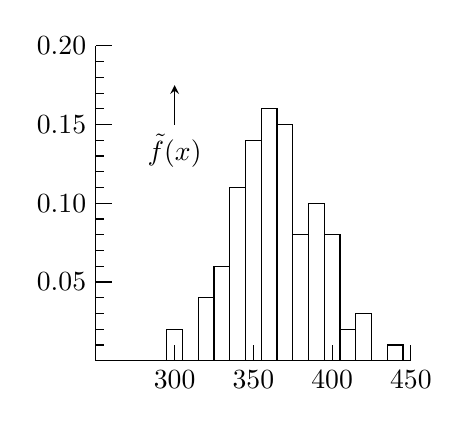
\begin{tikzpicture}
\pgfmathsetmacro{\w}{0.1}
\draw(0,0)--(4,0);
\draw(0,0)--(0,4);
\foreach \y/\ys in {1/0.05,2/0.10,3/0.15,4/0.20}{\draw(0,\y)node[left]{$\ys$}--++(0.2,0);}
\foreach \y in {0.2,0.4,0.6,0.8}{\draw(0,0+\y)--++(0.1,0)  (0,1+\y)--++(0.1,0) (0,2+\y)--++(0.1,0) (0,3+\y)--++(0.1,0);}
\foreach \x/\xs in {1/300,2/350,3/400,4/450}{\draw(\x,0)node[below]{$\xs$}--++(0,0.2);}
\draw(1-\w,0)--++(0,0.4)--++(2*\w,0)--++(0,-0.4);
\draw(1.4-\w,0)--++(0,0.8)--++(2*\w,0);
\draw(1.6-\w,0)--++(0,1.2)--++(2*\w,0);
\draw(1.8-\w,0)--++(0,2.2)--++(2*\w,0);
\draw(2-\w,0)--++(0,2.8)--++(2*\w,0);
\draw(2.2-\w,0)--++(0,3.2)--++(2*\w,0)--++(0,-0.2);
\draw(2.4-\w,0)--++(0,3)--++(2*\w,0)--++(0,-1.4);
\draw(2.6-\w,0)--++(0,1.6)--++(2*\w,0);
\draw(2.8-\w,0)--++(0,2)--++(2*\w,0)--++(0,-0.4);
\draw(3-\w,0)--++(0,1.6)--++(2*\w,0)--++(0,-1.2);
\draw(3.2-\w,0)--++(0,0.4)--++(2*\w,0);
\draw(3.4-\w,0)--++(0,0.6)--++(2*\w,0)--++(0,-0.6);
\draw(3.8-\w,0) rectangle ++(2*\w,0.2);
\draw[-stealth](1,3)node[below]{$\tilde{f}(x)$}--++(0,0.5);
\end{tikzpicture}
\caption*{(پ) تعددی مستطیلی ترسیم}
\end{subfigure}%
\begin{subfigure}{0.5\textwidth}
\centering
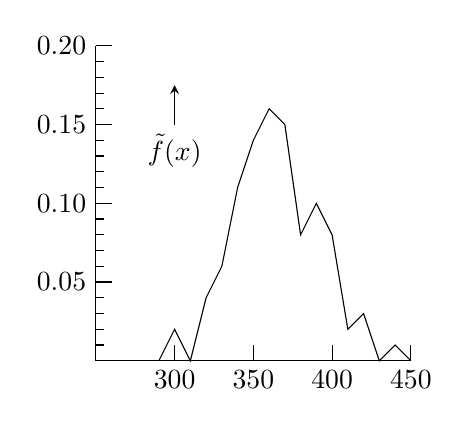
\begin{tikzpicture}
\pgfmathsetmacro{\w}{0.1}
\draw(0,0)--(4,0);
\draw(0,0)--(0,4);
\foreach \y/\ys in {1/0.05,2/0.10,3/0.15,4/0.20}{\draw(0,\y)node[left]{$\ys$}--++(0.2,0);}
\foreach \y in {0.2,0.4,0.6,0.8}{\draw(0,0+\y)--++(0.1,0)  (0,1+\y)--++(0.1,0) (0,2+\y)--++(0.1,0) (0,3+\y)--++(0.1,0);}
\foreach \x/\xs in {1/300,2/350,3/400,4/450}{\draw(\x,0)node[below]{$\xs$}--++(0,0.2);}
\draw(0.8,0)--(1,0.4)--(1.2,0)--(1.4,0.8)--(1.6,1.2)--(1.8,2.2)--(2,2.8)--(2.2,3.2)--(2.4,3)--(2.6,1.6)--(2.8,2)--(3,1.6)--(3.2,0.4)--(3.4,0.6)--(3.6,0)--(3.8,0.2)--(4,0);
\draw[-stealth](1,3)node[below]{$\tilde{f}(x)$}--++(0,0.5);
\end{tikzpicture}
\caption*{(ت) تعددی کثیر الاضلاع ترسیم}
\end{subfigure}%
\caption{ترسیم برائے جدول \حوالہ{جدول_شماریات_تعددی_تقسیم_الف}}
\label{شکل_شماریات_تعددی_ترسیم}
\end{figure}


نمونہ کا \موٹا{ترسیمی اظہار} شکل \حوالہ{شکل_شماریات_تعددی_ترسیم}-الف تا شکل \حوالہ{شکل_شماریات_تعددی_ترسیم}-ت میں دکھایا گیا ہے۔شکل \حوالہ{شکل_شماریات_تعددی_ترسیم}-پ میں ہر مستطیل کا رقبہ مطابقتی اضافی تعدد کے برابر  ہو گا لہٰذا عمودی محدد پر اضافی تعدد فی اکائی رقبہ ہو گا۔چونکہ شکل \حوالہ{شکل_شماریات_تعددی_ترسیم}-پ میں تمام مستطیل کی چوڑائی ایک جیسی ہے  لہٰذا عمودی محدد پر قیمتیں \عددی{\tilde{f}(x)} کے راست متناسب ہوں گی۔ البتہ مستطیل کو چوڑائیاں مختلف ہونے کی صورت میں ایسا نہیں ہو گا۔ شکل \حوالہ{شکل_شماریات_تعددی_ترسیم}-ت میں بھی یہی صورت حال ہو گی۔

ہم اب درج ذیل تفاعل متعارف کرتے ہیں
\begin{align*}
\tilde{F}(x)=\text{\RL{\عددی{x} اور \عددی{x} سے کم تمام قیمتوں کے اضافی تعدد کا مجموعہ}}
\end{align*}
جس کو \اصطلاح{نمونے کا مجموعی  تعددی تفاعل}\فرہنگ{تعددی!نمونے کا مجموعی تفاعل}\حاشیہب{cumulative frequency function of the sample}\فرہنگ{frequency!cumulative function of sample} یا مختصراً \اصطلاح{تقسیمی تفاعل نمونہ}\فرہنگ{تقسیمی تفاعل نمونہ}\فرہنگ{تقسیم!تقسیمی تفاعل نمونہ}\حاشیہب{sample distribution function}\فرہنگ{sample distribution function} کہتے ہیں۔شکل \حوالہ{شکل_شماریات_مجموعی_تعددی_تفاعل} میں مثال دی گئی ہے۔

\begin{figure}
\centering
\begin{subfigure}{1\textwidth}
\centering
\begin{tikzpicture}[x={2cm},y={0.5cm}]
\draw(0,4)--(0,0)--(5,0)node[right]{$x$};
\foreach \y/\ys in {2/0.1,4/0.2}{\draw(0,\y)node[left]{$\ys$}--++(0.2,0);}
\foreach \y in {1,3}{\draw(0,\y)--++(0.1,0);}
\foreach \x/\y in {1/0.2,1.4/0.8,1.6/1.2,1.8/2.2,2/2.8,2.2/3.2,2.4/3,2.6/1.6,2.8/2,3/1.6,3.2/0.4,3.4/0.6,3.8/0.2}{\draw(\x,0)--++(0,\y);}
\draw[-stealth](0.5,3)node[below]{$\tilde{f}(x)$}--++(0,0.5);
\end{tikzpicture}
\end{subfigure}
\begin{subfigure}{1\textwidth}
\centering
\begin{tikzpicture}[x={2cm},y={5cm}]
\draw(0,1)--(0,0)--(5,0)node[right]{$x$};
\foreach \y in {0.2,0.4,0.6,0.8}{\draw(0,0.5*\y)--++(0.1,0)  (0,0.5+0.5*\y)--++(0.1,0);}
\foreach \y in {0.5,1}{\draw(0,\y)node[left]{$\y$}--++(0.2,0);}
\foreach \x/\xs in {1/300,2/350,3/400,4/450}{\draw(\x,0)node[below]{$\xs$}--++(0,0.02);}
\foreach \x in {0.2,0.4,0.6,0.8} {\draw(\x,0)--++(0,0.01) (1+\x,0)--++(0,0.01)  (2+\x,0)--++(0,0.01) (3+\x,0)--++(0,0.01)  (4+\x,0)--++(0,0.01);}
\draw[-stealth](0.5,0.75)node[below]{$\tilde{F}(x)$}--++(0,0.2);
\draw(1,0)--(1,0.02)--(1.4,0.02)--(1.4,0.06)--(1.6,0.06)--(1.6,0.12)--(1.8,0.12)--(1.8,0.23)--(2,0.23)--(2,0.37)--(2.2,0.37)--(2.2,0.53)--(2.4,0.53)--(2.4,0.68)--(2.6,0.68)--(2.6,0.76)--(2.8,0.76)--(2.8,0.86)--(3,0.86)--(3,0.94)--(3.2,0.94)--(3.2,0.99)--(3.8,0.99)--(3.8,1)--(5,1);
\end{tikzpicture}
\end{subfigure}%
\caption{تعددی تفاعل \عددی{\tilde{f}(x)} اور مجموعی تعددی تفاعل \عددی{\tilde{F}(x)} برائے جدول \حوالہ{جدول_شماریات_تعددی_تقسیم_الف}}
\label{شکل_شماریات_مجموعی_تعددی_تفاعل}
\end{figure}

\عددی{\tilde{F}(x)} \ترچھا{سیڑھی تفاعل} (ٹکڑوں میں مستقل تفاعل) ہے جس میں ٹھیک ان \عددی{x}  پر جہاں \عددی{\tilde{f}(x)\ne0} ہو \عددی{\tilde{f}(x)} کے برابر چلانگ پائے جاتے ہیں۔پہلی چھلانگ نمونہ کی کم سے کم قیمت اور آخری چھلانگ نمونہ کی زیادہ سے زیادہ قیمت پر پائی جائے گی۔ آخری چھلانگ  کے بعد \عددی{\tilde{F}(x)=1} رہے گا۔

\عددی{\tilde{f}(x)} اور \عددی{\tilde{F}(x)} کا تعلق درج ذیل ہے
\begin{align}
\tilde{F}(x)=\sum_{t\le x}\tilde{f}(t)
\end{align}
جہاں \عددی{t\le x} کا مطلب  ہے کہ کسی بھی \عددی{x} کے لئے ان تمام \عددی{\tilde{f}(x)} کا مجموعہ لیا جائے گا جن کے لئے \عددی{t} کی قیمت \عددی{x} کے برابر یا \عددی{x} سے کم ہو۔

اگر کسی نمونہ میں مختلف اعداد کی تعداد بہت زیادہ ہو تب اس کا جدولی اور ترسیمی  اظہار غیر ضروری طور پر مشکل ہو گا جس کو \اصطلاح{گروہ بندی}\فرہنگ{گروہ بندی}\حاشیہب{grouping}\فرہنگ{grouping} سے آسان بنانا ممکن ہے۔آئیں گروہ بندی کے عمل کو سمجھیں۔

دیے گئے نمونہ کے لحاظ سے ہم ایسا وقفہ \عددی{I} منتخب کرتے ہیں جس میں تمام نمونی  قیمتیں شامل ہوں۔ہم \عددی{I} کو ٹکڑوں میں تقسیم کرتے ہیں جنہیں \اصطلاح{جماعتی وقفہ}\فرہنگ{جماعتی!وقفہ}\حاشیہب{class intervals}\فرہنگ{class!intervals} کہتے ہیں۔ان جماعتی وقفوں کے وسطی نقطوں کو \اصطلاح{جماعتی وسطی نقطے}\فرہنگ{جماعتی!وسطی نقطہ}\حاشیہب{class midpoints}\فرہنگ{class!midpoints} یا \اصطلاح{جماعتی نشان}\فرہنگ{جماعتی!نشان}\حاشیہب{class marks}\فرہنگ{class!marks} کہتے ہیں۔ہر جماعتی وقفہ میں پائے جانے والے نمونی قیمتیں کو \اصطلاح{طبقہ}\فرہنگ{طبقہ}\حاشیہب{class}\فرہنگ{class} کہتے ہیں۔ طبقہ  میں نمونی قیمتوں کی تعداد کو \اصطلاح{جماعتی تعدد}\فرہنگ{جماعتی!تعدد}\حاشیہب{class frequency}\فرہنگ{class!frequency} کہتے ہیں جس کو جسامت نمونہ \عددی{n} سے تقسیم کرنے سے \اصطلاح{اضافی جماعتی تعدد}\فرہنگ{جماعتی!اضافی تعدد}\حاشیہب{relative class frequency}\فرہنگ{class!relative frequency} حاصل ہو گا۔ اس تعدد \عددی{\tilde{f}(x)} کو جو جماعتی نشان کے تابع ہے  \اصطلاح{گروہ بند نمونہ کا تعددی تفاعل}\فرہنگ{تعددی! تفاعل، گروہ بند نمونہ}\حاشیہب{frequency function of the grouped sample}\فرہنگ{frequency!function of the grouped sample} کہتے ہیں۔اسی طرح  مجموعی اضافی جماعتی تعدد \عددی{\tilde{F}(x)} جو جماعتی نشان کے تابع ہے \اصطلاح{گروہ بند نمونہ کا تقسیمی تفاعل}\فرہنگ{تقسیمی!تفاعل،گروہ بند نمونہ}\فرہنگ{distribution function of the grouped sample}\حاشیہب{distribution!function of the grouped sample} کہلاتا ہے۔جدول \حوالہ{جدول_شماریات_دھاگہ_مضبوطی} اور جدول \حوالہ{جدول_شماریات_تعددی_گروہ_بند} میں مثال دیا گیا ہے۔
\begin{table}
\caption{کپاس کے سوتی دھاگے کو توڑنے کے لئے درکار قوت (نیوٹن میں)}
\label{جدول_شماریات_دھاگہ_مضبوطی}
\centering
\begin{otherlanguage}{english}
\begin{tabular}{RRRRRRRRRR}
\hline
114&118&86&107&87&94&82&81&98&84\\
120&126&98&89&114&83&94&106&96&111\\
123&110&83&118&83&96&96&74&91&81\\
102&107&103&80&109&71&96&91&86&129\\
130&104&86&121&96&96&127&94&102&87\\
\hline
\end{tabular}
\end{otherlanguage}
\end{table}

\begin{table}
\caption{تعددی جدول برائے جدول \حوالہ{جدول_شماریات_دھاگہ_مضبوطی} (گروہ بند)}
\label{جدول_شماریات_تعددی_گروہ_بند}
\centering
\begin{otherlanguage}{english}
\begin{tabular}{R|C|L|R|R|R}
\hline
\multirow{2}{*}{\text{\RL{\urdufont{جماعتی وقفہ}}}}&\text{\RL{\urdufont{جماعتی نشان}}}&\multicolumn{2}{C|}{\text{\RL{\urdufont{مطلق تعدد}}}}&\multirow{2}{*}{$\tilde{f}(x)$}&\multirow{2}{*}{$\tilde{F}(x)$}\\
\cline{3-4}
&x&\text{\RL{\urdufont{نشان شمار}}}&&&\\
\hline
65- 75&70&\kStrokeTwo&2&0.04&0.04\\
75- 85&80&\kStrokeFive\,\,\kStrokeThree&8&0.16&0.20\\
85- 95&90&\kStrokeFive\,\,\kStrokeFive\,\,\kStrokeOne&11&0.22&0.42\\
95-105&100&\kStrokeFive\,\,\kStrokeFive\,\,\kStrokeTwo&12&0.24&0.66\\
105-115&110&\kStrokeFive\,\,\kStrokeThree&8&0.16&0.82\\
115-125&120&\kStrokeFive&5&0.10&0.92\\
125-135&130&\kStrokeFour&4&0.08&1.00\\
\hline
&&\text{\urdufont{مجموعہ}}&50&1.00&\\
\hline
\end{tabular}
\end{otherlanguage}
\end{table}

جماعتوں کی تعداد جتنی کم رکھی جائے، گروہ بند نمونہ کی تقسیم اتنی  سادہ ہو گی اور اتنی ہی زیادہ معلومات کھوئی جائے گی چونکہ اصل نمونی قیمتیں اب صریحاً نظر نہیں آئیں گی۔گروہ بندی کرتے وقت دھیان رکھیں کہ صرف غیر ضروری معلومات کھوئی جائے۔ گروہ بند نمونہ استعمال کرتے ہوئے مشکلات سے بچنے کی خاطر درج ذیل اصولوں کا خیال رکھیں۔
\begin{itemize}
\item
جماعتی وقفے برابر رکھیں۔
\item
جماعتی نشان یوں منتخب کریں کہ جماعتی نشان سادہ اعداد (جن میں غیر صفر ہندسوں کی تعداد کم سے کم ہو) پر واقع ہوں۔
\item
اگر نمونی قیمت \عددی{x_j} دو جماعتوں کی سرحد پر واقع ہو تب یہ قیمت اس طبقہ میں شامل کیا جائے گا جو \عددی{x_j} سے شروع ہوتا ہو۔ 
\end{itemize}

%==========================
\حصہء{سوالات}
%==============
سوال \حوالہ{سوال_شماریات_ترسیم_الف} تا سوال \حوالہ{سوال_شماریات_ترسیم_ب} میں دیے گئے نمونہ کا تعددی جدول بنائیں اور نمونہ کو تعددی نقطہ ترسیم، ڈبہ ترسیم اور مستطیل ترسیم کی صورت میں دکھائیں۔

%==================
\ابتدا{سوال}\شناخت{سوال_شماریات_ترسیم_الف}\quad مزاحمت کی قیمت اوہم \عددی{\si{\ohm}} میں۔
\begin{align*}
\begin{array}{rrrrrrrrrr}
99&100&102&101&98&103&100&102&99&101\\
100&100&99&101&100&102&99&101&98&100
\end{array}
\end{align*}

\انتہا{سوال}
%====================
\ابتدا{سوال}\شناخت{سوال_شماریات_درکار_ترسیم_ت}\quad 
\begin{align*}
\begin{array}{rrrrrrrrrrrrrrr}
6& 2& 4& 1& 2& 4& 3& 3& 2& 1& 6& 5& 6& 3& 4
\end{array}
\end{align*}

\انتہا{سوال}
%========================
\ابتدا{سوال}\شناخت{سوال_شماریات_ترسیم_پ}\quad برقی سوئچ کا سیکنڈوں میں دورانیہ ردعمل 
\begin{align*}
\begin{array}{rrrrrrrrrr}
1.3&1.4&1.1&1.5&1.4&1.3&1.2&1.4&1.5&1.3\\
1.2&1.3&1.5&1.4&1.4&1.6&1.3&1.5&1.1&1.4
\end{array}
\end{align*}
\انتہا{سوال}
%=============================
\ابتدا{سوال}\شناخت{سوال_شماریات_درکار_ترسیم_ٹ}\quad خام کوئلہ میں کوئلہ کی فی صد مقدار
\begin{align*}
\begin{array}{rrrrrrrrrr}
87&86&85&87&86&87&86&81&77&85\\
86&84&83&83&82&84&83&79&82&73
\end{array}
\end{align*}
\انتہا{سوال}
%=============================
\ابتدا{سوال}\quad چادری فولاد کی تنشی مضبوطی [\si{\kilo\gram\per\milli\meter\squared}]
\begin{align*}
\begin{array}{rrrrrrrrrrrrrrr}
44&43&41&41&44&44&43&44&42&45&43&43&44&45&46\\
42&45&41&44&44&43&44&46&41&43&45&45&42&44&44
\end{array}
\end{align*}
\انتہا{سوال}
%=============================
\ابتدا{سوال}\quad  خود کار نظام سے \عددی{100} کاغذ  کے گھٹے بنانے میں کمی بیشی
\begin{align*}
\begin{array}{rrrrrrrrrr}
0&-1&0&0&1&1&2&0&1&0
\end{array}
\end{align*}
\انتہا{سوال}
%=============================
\ابتدا{سوال}\quad  ایک ہی قسم کے گاڑیوں کا تیل کا خرچہ۔  [کلومیٹر فی لیٹر]  
\begin{align*}
\begin{array}{rrrrrr}
12& 11.5&11&12.5&11&12
\end{array}
\end{align*}
\انتہا{سوال}
%=============================
\ابتدا{سوال}\quad  خود کار نظام سے بھری گئی تھیلوں کا گرام میں وزن
\begin{align*}
\begin{array}{rrrrrrrr}
200&203&199&198&201&200&201&201
\end{array}
\end{align*}
\انتہا{سوال}
%=============================
\ابتدا{سوال}\شناخت{سوال_شماریات_ترسیم_ب}\quad  اندرون شہر چلتی ریل گاڑی کا اڈے پر ٹھیک وقت پر پہنچنے سے انحراف (منٹوں میں)\حاشیہد{امید کی جا سکتی ہے کہ ایک دن ہماری ریل گاڑیاں بھی وقت کی اتنی پابند ہوں گی۔}
\begin{align*}
\begin{array}{rrrrrrrrrr}
3&4&1&0&2&2&3&1&5&3
\end{array}
\end{align*}
\انتہا{سوال}
%=============================
\ابتدا{سوال}\شناخت{سوال_شماریات_درکار_الف}\quad
سوال \حوالہ{سوال_شماریات_ترسیم_پ} کے نمونہ کی مجموعی تعددی تفاعل کا ترسیم کھینچیں۔
\انتہا{سوال}
%===========================
\ابتدا{سوال}\quad
جدول \حوالہ{جدول_شماریات_تعددی_گروہ_بند} کے گروہ بند نمونہ کا ڈبہ ترسیم، مستطیل ترسیم اور تعددی کثیر الاضلاع ترسیم کھینچیں۔ 
\انتہا{سوال}
%======================
\ابتدا{سوال}\quad
جدول \حوالہ{جدول_شماریات_کنکریٹ_بیلن} میں جماعتی وقفوں کے جماعتی نشان \عددی{300}، \عددی{320}، \عددی{340}، \نقطے پر لیتے ہوئے مطابقتی تعددی جدول بنائیں۔اس کے مستطیل ترسیم کھینچ کا شکل \حوالہ{شکل_شماریات_تعددی_ترسیم}-پ کے ساتھ موازنہ کریں۔
\انتہا{سوال}
%===========================
\ابتدا{سوال}\quad
جدول \حوالہ{جدول_شماریات_دھاگہ_مضبوطی} میں جماعتی نشان \عددی{75}، \عددی{85}، \عددی{95}، \نقطے لے کر مطابقتی تعددی جدول بنائیں۔اس کے مستطیل ترسیم کا سوال \حوالہ{سوال_شماریات_درکار_الف} کے ترسیم سے موازنہ کریں۔  
\انتہا{سوال}
%===================
\ابتدا{سوال}\quad
\عددی{1500} تجرباتی نتائج میں سب سے کم ناپ \عددی{\SI{10.8}{\centi\meter}} اور سب سے زیادہ ناپ \عددی{\SI{11.9}{\centi\meter}} تھی۔اس مواد کی گروہ بندی لے لئے جماعتی وقفہ تجویز کریں۔
\انتہا{سوال}
%==================

\حصہ{نمونی اوسط اور نمونی تغیریت}\شناخت{حصہ_شماریات_نمونی_اوسط_نمونی_تغیریت}
تعددی تفاعل (یا تقسیمی تفاعل) نمونہ کی صحیح تصویر کشی کرتا ہے۔اس تفاعل سے ہم نمونہ کے کئی خواص کا حساب لگا سکتے ہیں مثلاً نمونی قیمتوں کی اوسط جسامت، پھیل، تشاکل، وغیرہ۔ اس حصہ میں ہم ایسے اہم ترین دو قیمتوں، نمونی اوسط اور نمونی تغیریت، پر غور کریں گے۔

نمونہ \عددی{x_1,x_2,\cdots,x_n} کی اوسط قیمت یا مختصراً \اصطلاح{نمونی اوسط}\فرہنگ{نمونی!اوسط}\فرہنگ{اوسط}\حاشیہب{sample mean}\فرہنگ{sample!mean} کو \عددی{\bar{x}} سے ظاہر کیا جاتا ہے جس کی تعریف درج ذیل کلیہ دیتی ہے۔
\begin{align}\label{مساوات_شماریات_نمونی_اوسط_الف}
\bar{x}=\frac{1}{n}\sum_{j=1}^{n}x_j=\frac{1}{n}(x_1+x_2+\cdots+x_n)
\end{align}
تمام نمونی قیمتوں کے مجموعہ کو جسامت \عددی{n} سے تقسیم کرتے ہوئے نمونی اوسط حاصل ہو گا۔ظاہر ہے کہ یہ نمونی قیمتوں کی اوسط جسامت دے گا۔

نمونہ \عددی{x_1,x_2,\cdots,x_n} کی \اصطلاح{نمونی تغیریت}\فرہنگ{نمونی!تغیریت}\فرہنگ{تغیریت}\حاشیہب{sample variance}\فرہنگ{sample!variance} کو \عددی{s^2} سے ظاہر کیا جاتا ہے جس کی تعریف درج ذیل کلیہ دیتی ہے۔
\begin{gather}
\begin{aligned}\label{مساوات_شماریات_نمونی_اوسط_ب}
s^2&=\frac{1}{n-1}\sum_{j=1}^{n}(x_j-\bar{x})^2\\
&=\frac{1}{n-1}[(x_1-\bar{x})^2+(x_2-\bar{x})^2+\cdots +(x_n-\bar{x})^2]
\end{aligned}
\end{gather}
نمونی اوسط \عددی{\bar{x}} سے نمونی قیمتوں کے انحراف کے مربعوں کو \عددی{n-1} سے تقسیم کرتے ہوئے نمونی تغیریت حاصل ہو گی۔یہ نمونی قیمتوں کی انحراف یا پھیل کی ناپ ہے۔نمونی تغیریت غیر منفی عدد ہو گا۔ نمونی تغیریت \عددی{s^2} کا مثبت جذر \اصطلاح{معیاری انحراف}\فرہنگ{معیاری انحراف}\حاشیہب{standard deviation}\فرہنگ{standard deviation} کہلاتا ہے جس کو \عددی{s} سے ظاہر کیا جاتا ہے۔

%=================
\ابتدا{مثال}\شناخت{مثال_شماریات_اوسط}\quad \موٹا{نمونی اوسط اور نمونی تغیریت}\\
بلا منصوبہ منتخب کیے گئے کیلوں کی  (سنٹی میٹروں میں) لمبائیاں درج ذیل ہیں۔
\begin{align*}
\begin{array}{cccccccccc}
0.80&0.81&0.81&0.82&0.81&0.82&0.80&0.82&0.81&0.81
\end{array}
\end{align*}
مساوات \حوالہ{مساوات_شماریات_نمونی_اوسط_الف} سے نمونی اوسط
\begin{align*}
\bar{x}=\frac{1}{10}(0.80+0.81+0.81+0.82+\cdots+0.81)=\SI{0.811}{\centi\meter}
\end{align*}
اور مساوات \حوالہ{مساوات_شماریات_نمونی_اوسط_ب} سے نمونی تغیریت
\begin{align*}
s^2=\frac{1}{9}[(0.80-0.811)^2+\cdots+(0.81-0.811)^2]=\SI{0.000054}{\centi\meter\squared}
\end{align*}
ہے۔ایک جیسی نمونی قیمتوں کو اکٹھا لکھنے سے حساب نسبتاً آسان بنایا جا سکتا ہے جیسے
\begin{align*}
\bar{x}=\frac{1}{10}(2\cdot 0.80+5\cdot 0.81+3\cdot 0.82)=\SI{0.811}{\centi\meter}
\end{align*} 
جہاں قوسین میں تین مختلف نمونی قیمتوں \عددی{x_1=0.80}، \عددی{x_2=0.81} اور \عددی{x_3=0.82} کو ان کی تعدد سے ضرب دیا گیا ہے۔اسی طرح
\begin{align*}
s^2=\frac{1}{9}[(2(0.800-0.811)^2+5(0.810-0.811)^2+3(0.820-0.811)^2]=\num{0.000054}
\end{align*}
ہو گا۔
\انتہا{مثال}
%=========================
اس مثال میں ہم نے \عددی{\bar{x}} اور \عددی{s^2} کو نمونہ کے تعددی تفاعل \عددی{\tilde{f}(x)} کی مدد سے حاصل کرنا دیکھا۔اگر ایک نمونہ میں ٹھیک \عددی{m} مختلف اعدادی قیمتیں 
\begin{align*}
x_1, x_2,\cdots, x_m
\end{align*}
پائی جاتی ہوں جن کے مطابقتی اضافی تعدد
\begin{align*}
\tilde{f}(x_1),\tilde{f}(x_2),\cdots,\tilde{f}(x_m)
\end{align*}
ہوں تب حساب کے لئے درکار تعدد درج ذیل ہوں گے
\begin{align*}
n\tilde{f}(x_1),n\tilde{f}(x_2),\cdots,n\tilde{f}(x_m)
\end{align*}
جنہیں استعمال کرتے ہوئے مساوات \حوالہ{مساوات_شماریات_نمونی_اوسط_الف} اور مساوات \حوالہ{مساوات_شماریات_نمونی_اوسط_ب} سے
\begin{align}\label{مساوات_شماریات_نمونی_اوسط_پ}
\bar{x}=\frac{1}{n}\sum_{j=1}^{m}x_jn\tilde{f}(x_j)
\end{align}
اور
\begin{align}\label{مساوات_شماریات_نمونی_اوسط_ت}
s^2=\frac{1}{n-1}\sum_{j=1}^{m} (x_j-\bar{x})^2n\tilde{f}(x_j)
\end{align}
حاصل ہو گا۔ دھیان رہے کہ مساوات \حوالہ{مساوات_شماریات_نمونی_اوسط_الف} اور مساوات \حوالہ{مساوات_شماریات_نمونی_اوسط_ب} میں ہم تمام نمونی قیمتوں پر مجموعہ لیتے ہیں جبکہ مساوات \حوالہ{مساوات_شماریات_نمونی_اوسط_پ} اور مساوات \حوالہ{مساوات_شماریات_نمونی_اوسط_ت} میں ہم اعدادی طور مختلف نمونی قیمتوں پر مجموعہ حاصل کرتے ہیں۔مطلق تعدد \عددی{n\tilde{f}(x_j)} عدد صحیح ہوں گے جبکہ اضافی تعدد \عددی{\tilde{f}(x_j)} عموماً غیر عدد صحیح ہوں گے۔

چونکہ \عددی{x_j-\bar{x}} کی مطلق قیمت نمونی اوسط کی نسبت بہت کم ہو سکتی ہے لہٰذا \عددی{s^2} کے مذکورہ بالا کلیات کی استعمال سے (خود کار حساب میں) ملحوظ ہندسے ضائع ہوں گے۔ہم \عددی{s^2} کا ایک ایسا کلیہ اخذ کرتے ہیں جو ان مشکلات سے دو چار نہ ہو۔ہم  مساوات \حوالہ{مساوات_شماریات_نمونی_اوسط_ب} میں
\begin{align*}
(x_j-\bar{x})^2=x_j^2-2x_j\bar{x}+\bar{x}^2
\end{align*}
پر کرتے ہوئے تین مجموعے 
\begin{align*}
\sum(x_j-\bar{x})^2=\sum x_j^2-2\bar{x}\sum x_j+\sum \bar{x}^2
\end{align*}
حاصل کرتے ہیں جہاں آخری مجموعہ \عددی{n\bar{x}^2} کے برابر ہے۔ مساوات \حوالہ{مساوات_شماریات_نمونی_اوسط_الف} سے \عددی{\bar{x}} کی قیمت پر کرتے ہوئے
\begin{align*}
-2\bar{x}\sum x_j=-\frac{2}{n}(\sum x_j)^2 \quad \text{اور}\quad n\bar{x}^2=\frac{1}{n}(\sum x_j)^2
\end{align*}
لکھا جا سکتا ہے جنہیں استعمال کرتے ہوئے
\begin{align}\label{مساوات_شماریات_نمونی_اوسط_ٹ}
s^2=\frac{1}{n-1}\big[\sum_{j=1}^{n}x_j^2-\frac{1}{n}\big(\sum_{j=1}^{n}x_j\big)^2\big]
\end{align}
حاصل ہو گا۔ اسی طرح  مساوات \حوالہ{مساوات_شماریات_نمونی_اوسط_ت} کو تبدیل کرتے ہوئے
\begin{align}\label{مساوات_شماریات_نمونی_اوسط_ث}
s^2=\frac{1}{n-1}\big[\sum_{j=1}^{m} x_j^2n\tilde{f}(x_j)-\frac{1}{n}\big(\sum_{j=1}^{m}x_jn\tilde{f}(x_j)\big)^2\big]
\end{align}
حاصل کیا جا سکتا ہے۔

مثال کے طور پر مثال \حوالہ{مثال_شماریات_اوسط} میں مساوات \حوالہ{مساوات_شماریات_نمونی_اوسط_پ} اور مساوات \حوالہ{مساوات_شماریات_نمونی_اوسط_ث} (جدول \حوالہ{جدول_شماریات_اوسط_تغیریت}) سے پہلے کی طرح \عددی{\bar{x}=\tfrac{8.11}{10}=0.811} اور  
\begin{align*}
s^2=\frac{1}{9}\big(6.5777-\frac{8.11^2}{10}\big)=\frac{\num{0.00049}}{9}=\num{0.000054}
\end{align*}
حاصل ہوتے ہیں۔
\begin{table}
\caption{اوسط اور تغیریت کا حساب برائے مثال \حوالہ{مثال_شماریات_اوسط}}
\label{جدول_شماریات_اوسط_تغیریت}
\centering
\begin{otherlanguage}{english}
\begin{tabular}{C|C|C|C|C}
\hline
\Tstrut
x_j&10\tilde{f}(x_j)&x_j\cdot 10 \tilde{f}(x_j)&x_j^2&x_j^2\cdot 10 \tilde{f}(x_j)\\
\hline
0.80&2&1.60&0.6400&1.2800\\
0.81&5&4.05&0.6561&3.2805\\
0.82&3&2.46&0.6724&2.0172\\
\hline
\end{tabular}
\end{otherlanguage}
\end{table}

%=======================
\حصہء{سوالات}
%=====================
\ابتدا{سوال}\quad
گزشتہ حصے کی سوال \حوالہ{سوال_شماریات_درکار_ترسیم_ت} کے لئے نمونی اوسط اور نمونی تغیریت تلاش کریں۔\\
جواب:\quad
$\bar{x}=3.47,\,\, s^2=2.98$
\انتہا{سوال}
%=======================
\ابتدا{سوال}\quad
گزشتہ حصے کی سوال \حوالہ{سوال_شماریات_درکار_ترسیم_ٹ} کے لئے نمونی اوسط اور نمونی تغیریت تلاش کریں۔\\
جواب:\quad
$\bar{x}=84,\,\,s^2=\tfrac{1251}{95}$
\انتہا{سوال}
%=======================
\ابتدا{سوال}\quad
نمونہ \عددی{2,1,4,5} کا مستطیل ترسیم کھینچیں۔ترسیم کو دیکھ کر \عددی{\bar{x}} اور \عددی{s} کی قیمتوں کا اندازہ لگائیں۔\عددی{\bar{x}}، \عددی{s^2} اور \عددی{s} کی قیمتوں کا حساب لگائیں۔\\
جواب:\quad
$\bar{x}=3,\,\, s^2=3.3,\,\, s=1.817$
\انتہا{سوال}
%=====================
\ابتدا{سوال}\quad
دکھائیں کہ کم سے کم اور زیادہ سے زیادہ نمونی قیمتوں کے بیچ \عددی{\bar{x}} ہو گا۔
\انتہا{سوال}
%===========================
\ابتدا{سوال}\quad \موٹا{نمونہ کا }\\
نمونہ میں سب سے بڑی قیمت اور سب سے چھوٹی قیمت کے فرق کو نمونہ کا \اصطلاح{}\فرہنگ{}\حاشیہب{range}\فرہنگ{range} کہتے ہیں۔مثال \حوالہ{مثال_شماریات_اوسط} میں دیے گئے نمونہ کا  تلاش کریں۔\\
جواب:\quad
$0.02$
\انتہا{سوال}
%==========================
\ابتدا{سوال}\quad \موٹا{صدویہ، وسطانیہ}\\
نمونہ کی \عددی{p} ویں \اصطلاح{صدویہ}\فرہنگ{صدویہ}\حاشیہب{percentile}\فرہنگ{percentile} سے مراد ایسا عدد \عددی{Q_p} ہے کہ کم از کم \عددی{p\,\si{\percent}} نمونی قیمتیں \عددی{Q_p} سے کم یا اس کے برابر ہوں اور ساتھ ہی \عددی{(100-p)\,\si{\percent}} نمونی قیمتیں اس سے زیادہ یا اس کے برابر ہوں۔اگر ایک سے زیادہ ایسا عدد پایا جاتا ہو (جس صورت میں ان اعداد کا وقفہ پایا جائے گا) تب \عددی{p} ویں صدویہ سے مراد ان اعداد کا اوسط (یعنی وقفے  کا وسطی نقطہ) ہو گا۔بالخصوص \عددی{Q_{50}} کو \اصطلاح{وسطانیہ}\فرہنگ{وسطانیہ}\حاشیہب{median}\فرہنگ{median} کہتے ہیں جس کو \عددی{\tilde{x}} سے ظاہر کیا جاتا ہے۔وسطانیہ کو \اصطلاح{نصف چوتھائی}\فرہنگ{چوتھائی!نصف}\حاشیہب{middle quartile}\فرہنگ{quartile!middle} بھی کہتے ہیں۔جدول \حوالہ{جدول_شماریات_تعددی_تقسیم_الف} کے نمونہ  کا وسطانیہ \عددی{\tilde{x}} تلاش کریں۔\\
جواب:\quad
$360$
\انتہا{سوال}
%==========================
\ابتدا{سوال}\شناخت{سوال_شماریات_چوتھائی_الف}\quad 
نمونہ کی \عددی{Q_{25}} اور \عددی{Q_{75}} صدویہ کو بالترتیب \اصطلاح{نچلی چوتھائی}\فرہنگ{چوتھائی!نچلی}\حاشیہب{lower quartile}\فرہنگ{quartile!lower} اور \اصطلاح{بالائی چوتھائی}\فرہنگ{چوتھائی!بالائی}\حاشیہب{upper quartile}\فرہنگ{quartile!upper} کہتے ہیں جبکہ \عددی{Q_{75}-Q_{25}} جو پھیل کی ناپ ہے کو \اصطلاح{چوتھائی }\فرہنگ{چوتھائی!}\حاشیہب{interquartile range}\فرہنگ{quartile!interquartile range} کہتے ہیں۔جدول \حوالہ{جدول_شماریات_تعددی_تقسیم_الف} کے نمونہ  کا کی \عددی{Q_{25}}، \عددی{Q_{75}} اور \عددی{Q_{75}-Q_{25}} تلاش کریں۔\\
جواب:\quad
$350,\,\,380,\,\,30$
\انتہا{سوال}
%=============================
\ابتدا{سوال}\quad
جدول \حوالہ{جدول_شماریات_دھاگہ_مضبوطی} کے لئے سوال \حوالہ{سوال_شماریات_چوتھائی_الف} کو حل کریں۔\\
جواب:\quad
$\tfrac{345}{4},\,\,\tfrac{439}{4},\,\,\tfrac{47}{2}$
\انتہا{سوال}
%=========================
\ابتدا{سوال}\quad \موٹا{عادہ}\\
نمونہ میں سب سے زیادہ بار آنے والی قیمت کو نمونہ کی \اصطلاح{عادہ}\فرہنگ{عادہ}\حاشیہب{mode}\فرہنگ{mode} کہتے ہیں۔یہ سب سے عام قدر ہوتی ہے۔درج ذیل نمونہ کی اوسط، وسطانیہ اور عادہ تلاش کریں۔ ان پر تبصرہ کریں۔
\begin{align*}
\begin{array}{L|CCC}
\text{\RL{\urdufont{قیمت}}}&100&1000&\num{1000000}\\
\hline
\text{\RL{\urdufont{تعدد}}}&100&90&20
\end{array}
\end{align*}
جواب:\quad
$\text{اوسط}=\num{10000},\,\, \text{وسطانیہ}=1000,\,\,\text{عادہ}=100$
\انتہا{سوال}
%===========================
\ابتدا{سوال}\شناخت{سوال_شماریات_مبدا_کام}\quad \موٹا{مبدا کام}\\
اگر \عددی{x_j=x^*_j+c} ہو جہاں  \عددی{j=1,\cdots,n} اور \عددی{c} کوئی مستقل ہو تب دکھائیں کہ
\begin{align*}
\bar{x}=c+\bar{x}^*,\quad \big(\bar{x}^*=\frac{1}{n}\sum_{j=1}^{n}x_j^*\big)\quad  \text{اور} \quad \quad s^2=s^{*2}
\end{align*}
ہوں گے جہاں \عددی{x_j^*} قیمتوں  کی تغیریت \عددی{s^{*2}} ہے۔(عملی استعمال میں \عددی{c} یوں منتخب کیا جاتا ہے کہ \عددی{x_j^*} کی مطلق قیمتیں چھوٹی ہوں۔جیومیٹریائی طور پر یہ مبدا کی تبدیلی کے مترادف ہے لہٰذا اس کو \ترچھا{ترکیب مبدا کام}\فرہنگ{ترکیب!مبدا کام}\حاشیہب{method of working origin}\فرہنگ{method!of working origin} کہتے ہیں۔)  
\انتہا{سوال}
%=========================
\ابتدا{سوال}\quad
ترکیب مبدا کام کو مثال \حوالہ{مثال_شماریات_اوسط} کے نمونہ پر لاگو کریں۔
\انتہا{سوال}
%====================
\ابتدا{سوال}\quad \موٹا{مکمل رمز نویسی}\\
اگر \عددی{x_j=c_1x_j^*+c_2} ہو جہاں \عددی{j=1,\cdots,n} جبکہ \عددی{c_1} اور \عددی{c_2} مستقل ہیں تب دکھائیں کہ
\begin{align*}
\bar{x}=c_1\bar{x}^*+c_2,\quad s^2=c_1^2s^{*2}
\end{align*}
ہوں گے جہاں \عددی{\bar{x}^*} اور \عددی{s^{*2}} کی معنی سوال \حوالہ{سوال_شماریات_مبدا_کام} میں پیش کی گئی ہیں۔اس کو \اصطلاح{ترکیب مکمل رمز نویسی}\فرہنگ{ترکیب!مکمل رمز نویسی}\حاشیہب{method of full coding}\فرہنگ{method!of full coding} کہتے ہیں۔(اس ترکیب سے قلم و کاغذ استعمال کرتے ہوئے نتائج کی جلد جانچ پڑتال کی جا سکتی ہے۔)
\انتہا{سوال}
%======================
\ابتدا{سوال}\quad
اس ترکیب کو مثال \حوالہ{مثال_شماریات_اوسط} کے نمونہ پر لاگو کریں۔
\انتہا{سوال}
%======================
\ابتدا{سوال}\quad
کسی بھی نمونہ کی گروہ بندی سے عموماً نمونی اوسط متاثر ہو گا۔دکھائیں کہ نمونی اوسط میں تبدیل \عددی{\tfrac{l}{2}} سے زیادہ نہیں ہو سکتی ہے جہاں ہر ایک جماعتی وقفہ کی لمبائی \عددی{l} ہے۔
\انتہا{سوال}
%=======================
\ابتدا{سوال}\quad
جدول \حوالہ{جدول_شماریات_دھاگہ_مضبوطی} کی غیر گروہ بند نمونہ کی گروہ بندی  جدول \حوالہ{جدول_شماریات_تعددی_گروہ_بند} میں کی گئی ہے۔دونوں مواد کی اوسط اور تغیریت تلاش کریں۔نتائج کا آپس میں موازنہ کریں۔\\
جواب:\quad
$\text{غیر گروہ بند}:\,\, \bar{x}=99.2,\,\, s^2=234.7;\quad \text{گروہ بند}:\,\, \bar{x}=99.4,\,\, s^2=254.7$
\انتہا{سوال}
%===========================

\حصہ{بلا منصوبہ تجربات، انجام، وقوعات}\شناخت{حصہ_شماریات_تجربات_انجام_وقوعات}
شماریاتی تجربات یا شماریاتی مشاہدے  سے ہمیں نمونے حاصل ہوں گے جن کی مدد سے ہم متعلقہ  آبادی کے بارے میں نتائج اخذ کرنا چاہیں گے۔ایسا کرنے سے پہلے  حسابی احتمال کی مدد سے ہمیں آبادی کے حسابی نمونے  بنانے ہوں گے۔یہ نظریہ حسابی شماریات کی بنیاد ہے جس کی گہرائی میں ہم اپنی ضرورت کے مطابق  جائیں گے۔اس حصہ میں کئی بنیادی تصورات کو متعارف کیا جائے گا۔

ایک بلا منصوبہ تجربہ یا بلا منصوبہ  مشاہدہ، جنہیں ہم مختصراً \اصطلاح{تجربہ}\فرہنگ{تجربہ}\حاشیہب{experiment}\فرہنگ{experiment} یا \اصطلاح{مشاہدہ}\فرہنگ{مشاہدہ}\حاشیہب{observation}\فرہنگ{observation} کہیں گے، سے مراد وہ عمل ہے جو درج ذیل خواص رکھتا ہو۔
\begin{itemize}
\item
اس کو طے شدہ قواعد کے تحت سرانجام دیا جاتا ہے جو عمل کو مکمل طور پر بیان کرتے ہیں۔
\item
اس  عمل کو جتنی بار چاہیں دوبارہ انجام  دیا جا سکتا ہے۔
\item
ہر مرتبہ عمل کا نتیجہ  اتفاق پر منحصر ہو گا (یعنی نتیجہ ان اثرات پر منحصر ہے جنہیں ہم قابو نہیں کر سکتے ہیں) لہٰذا قبل از وقت  یکتا طور پر نتیجہ جاننا ممکن نہیں ہو گا۔
\end{itemize} 

ایک مرتبہ تجربے کے عمل سے حاصل نتیجہ کو  اس \اصطلاح{کوشش}\فرہنگ{کوشش}\حاشیہب{trial}\فرہنگ{trial} کا  \اصطلاح{انجام}\فرہنگ{انجام}\حاشیہب{outcome}\فرہنگ{outcome} کہتے ہیں۔

اس کی مثال (کرکٹ کی کھیل کی آغاز میں) سکہ پھینکنا، \ترچھا{لوڈو}\حاشیہب{ludo} کی کھیل میں \ترچھا{پانسہ}\حاشیہد{ایک مکعب جس کی چھ سطحوں پر ایک تا چھ نقطے ہوتے ہیں۔} پھینکنا، \عددی{100} پیچ کی ڈبی سے \عددی{10} پیچوں کا انتخاب  یا مختلف حالات میں کیمیائی عمل کی  پیداوار تعین کرنا اور دیگر تجربات مثلاً  بلا منصوبہ \عددی{20} افراد کا انتخاب اور ان کا \اصطلاح{فشار خون}\فرہنگ{فشار خون}\حاشیہب{blood pressure}\فرہنگ{blood pressure} تعین کرنا یا کسی موضوع پر ان کی رائے جاننا ہیں۔

کسی تجربہ کے تمام ممکنہ انجام کے سلسلہ کو اس تجربہ کی \اصطلاح{نمونی فضا}\فرہنگ{نمونی!فضا}\حاشیہب{sample space}\فرہنگ{sample!space} کہتے ہیں جس کو \عددی{S} سے ظاہر کیا جائے گا۔ہر ایک انجام کو \عددی{S} کا \اصطلاح{رکن}\فرہنگ{رکن}\حاشیہب{element}\فرہنگ{element} یا \اصطلاح{نقطہ}\فرہنگ{نقطہ}\حاشیہب{point}\فرہنگ{point} کہتے ہیں۔متناہی تعداد کے ارکان پر مشتمل سلسلہ \اصطلاح{متناہی} جبکہ لامتناہی تعداد کے ارکان پر مشتمل سلسلہ \اصطلاح{لامتناہی} کہلائے گا۔ 

مثال کے طور پر پانسہ پھینکنے کے بلا منصوبہ تجربہ کے ساتھ درج ذیل نمونی سلسلہ منسلک کیا جا سکتا ہے، 
\begin{align*}
S=\{1,2,3,4,5,6\}
\end{align*}
چونکہ پانسہ پھینکنے کے بعد (چھ ممکنات میں سے) کسی ایک رخ رکے گا۔

صنعتی پیداوار سے ہم  ایک رکن نکال کر دیکھ سکتے ہیں کہ آیا وہ بے عیب یا عیب دار ہے۔یوں \عددی{S} دو ارکان \عددی{D} (عیب دار)  اور \عددی{N} (بے عیب)  پر مشتمل ہو گا جنہیں اعداد مثلاً \عددی{0} (عیب دار) اور \عددی{1} (بے عیب) سے بھی ظاہر کیا جا سکتا ہے۔اب اگر ہم ایک سے زیادہ اقسام کے عیب میں تمیز کریں تب نمونی فضا دو سے زائد نقطوں پر مشتمل ہو گا۔

کپاس کی مضبوطی کے تجربہ (جدول \حوالہ{جدول_شماریات_دھاگہ_مضبوطی}) میں نمونی فضا لامتناہی ہو گا چونکہ دھاگہ توڑنے کے لئے درکار قوت کسی مخصوص  میں کوئی بھی مثبت قیمت ہو سکتی ہے۔

عملی مسائل میں ہمیں انفرادی انجام سے زیادہ دلچسپی نہیں ہو گی بلکہ ہم صرف اتنا جاننا چاہیں گے کہ آیا اس کا کسی مخصوص سلسلہ انجام سے تعلق ہے (یا نہیں ہے)۔ظاہر ہے کہ ایسا ہر سلسلہ \عددی{A} پوری نمونی فضا \عددی{S} کا ذیلی سلسلہ  ہو گا۔اس کو \اصطلاح{وقوعہ}\فرہنگ{وقوعہ}\حاشیہب{event}\فرہنگ{event} کہتے ہیں۔ 

چونکہ کوئی بھی انجام \عددی{S} کا ذیلی سلسلہ ہو گا لہٰذا یہ ایک مخصوص قسم کا وقوعہ ہو گا جس کو \ترچھا{بنیادی وقوعہ}\فرہنگ{وقوعہ!بنیادی} کہتے ہیں۔اسی طرح پوری فضا \عددی{S} بھی ایک مخصوص وقوعہ ہے۔

%=====================
\ابتدا{مثال}\شناخت{مثال_شماریات_نلکے}\quad
پانچ پانی کے نلکوں (جنہیں ایک تا پانچ سے ظاہر کیا جاتا ہے) میں سے دو نلکے منتخب کیے جاتے ہیں۔نمونی فضا درج ذیل دس ممکنہ انجام پر مشتمل ہو گی۔
\begin{align*}
1,2\quad 1,3\quad 1,4\quad 1,5\quad 2,3\quad 2,4\quad 2,5\quad 3,4\quad 3,5\quad 4,5
\end{align*}
اب اگر ہم عیب دار نلکوں میں دلچسپی رکھتے ہوں تب ہمیں درج ذیل تین انجاموں میں فرق کرنا ہو گا۔
\begin{align*}
A:\text{\RL{کوئی بھی عیب دار نہیں ہے}},\quad B:\text{\RL{ایک عیب دار ہے}},\quad C:\text{\RL{دونوں عیب دار ہیں}}
\end{align*}
فرض کریں کہ نلکوں میں \عددی{1,2,3} عیب دار ہیں تب درج ذیل ہو گا۔
\begin{align*}
\text{\RL{منتخب کرنے سے \عددی{A} ہو گا}}\quad &4,5,\\
\text{\RL{منتخب کرنے سے \عددی{B} ہو گا}}\quad &1,4\quad 1,5\quad 2,4\quad 2,5\quad 3,4\quad 3,5\\
\text{\RL{منتخب کرنے سے \عددی{C} ہو گا}}\quad &1,2\quad 1,3\quad 2,3
\end{align*} 
\انتہا{مثال}
%==========================

نمونی فضا \عددی{S} اور تجربہ کے انجام کو \اصطلاح{وین اشکال}\فرہنگ{وین اشکال}\حاشیہب{Venn diagram}\فرہنگ{Venn diagram} سے ظاہر کیا جا سکتا ہے۔ فرض کریں کہ  شکل \حوالہ{شکل_شماریاتی_وین_شکل_الف} میں چکور کے اندر نقطوں کا سلسلہ \عددی{S} کو ظاہر کرتے ہے۔تب مستطیل کے اندر بند منحنی کا اندرون کسی وقوعہ کو ظاہر کرے گا جس کو ہم \عددی{E}  سے ظاہر کرتے ہیں۔ ان تمام ارکان (انجاموں) کا سلسلہ جو \عددی{E} میں شامل نہیں ہیں کو \عددی{S} میں \عددی{E} کا متمم کہتے ہیں جس کو \عددی{E^c}\حاشیہد{یا \عددی{\bar{E}} سے ظاہر کیا جاتا ہے جس کو ہم استعمال نہیں کریں گے چونکہ اس کو کسی دوسرے مقصد (بندش سلسلہ) کے لئے مختص کیا گیا ہے۔} سے ظاہر کیا گیا ہے۔  
\begin{figure}
\centering
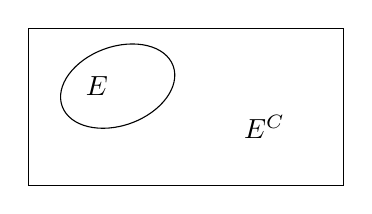
\begin{tikzpicture}
\draw(0,0) rectangle (4,2);
\draw[rotate=20](1.5,0.8)node[left]{$E$} circle (0.75cm and 0.5cm);
\draw(3,0.75)node[]{$E^C$};
\end{tikzpicture}
\caption{وین شکل میں نمونی سلسلہ \عددی{S} اور وقوعات \عددی{E} اور \عددی{E^C} دکھائے گئے ہیں}
\label{شکل_شماریاتی_وین_شکل_الف}
\end{figure}

مثال کے طور پر پانسہ پھینکنے کے تجربہ میں 
\begin{align*}
E:\quad \text{\RL{جب جفت عدد حاصل ہو}}
\end{align*}
کا متمم
\begin{align*}
E^C:\quad \text{\RL{جب طاق عدد حاصل ہو}}
\end{align*}
ہو گا۔ایسا وقوعہ جس میں کوئی انجام نہ پایا جاتا ہو کو \ترچھا{خالی وقوعہ}\فرہنگ{وقوعہ!خالی}\حاشیہب{empty event}\فرہنگ{event!empty} یا \اصطلاح{نا ممکن وقوعہ}\فرہنگ{وقوعہ!نا ممکن}\حاشیہب{impossible event}\فرہنگ{event!impossible} کہتے ہیں جس کو \عددی{\varnothing} سے ظاہر کیا جاتا ہے۔

فرض کریں کہ کسی تجربہ میں \عددی{A} اور \عددی{B} کوئی دو وقوعات ہیں۔تب  وہ وقوعہ جو \عددی{S} میں ان تمام ارکان پر مشتمل ہو جو \عددی{A} یا \عددی{B} یا دونوں میں پائے جاتے ہوں کو \عددی{A} اور \عددی{B} کا  \اصطلاح{اشتراک}\فرہنگ{اشتراک}\حاشیہب{union}\فرہنگ{union} کہلاتا ہے جس کو درج ذیل سے ظاہر کیا جاتا ہے۔
\begin{align*}
A\cup B
\end{align*} 
وہ وقوعہ جو \عددی{S} میں ان تمام ارکان پر مشتمل ہو جو \عددی{A} اور \عددی{B} دونوں میں پائے جاتے ہوں کو \عددی{A} اور \عددی{B} کا \اصطلاح{تقاطع}\فرہنگ{تقاطع}\حاشیہب{intersection}\فرہنگ{intersection} کہلاتا ہے جس کو درج ذیل سے ظاہر کیا جاتا ہے۔شکل \حوالہ{شکل_شماریات_وین_شکل_اشتراک_تقاطع} میں اشتراک اور تقاطع کو وین شکل پر دکھایا گیا ہے۔
\begin{align*}
A\cap B
\end{align*} 
%=================
\begin{figure}
\centering
\begin{subfigure}{0.5\textwidth}
\centering
\begin{tikzpicture}
\def\firstCircle{(0.75,1.75) circle (0.75cm and 0.5cm)};
\def\secondCircle{(1.5,1.5) circle (0.75cm and 0.5cm)}
%
\begin{scope}[even odd rule]
\clip  (0,0) rectangle (3,2) [rotate=-20] \firstCircle  ;
\fill[lgray,rotate=-20] \secondCircle;
\end{scope}
\fill[lgray,rotate=-20]\firstCircle;
\draw[rotate=-20](0.75,1.75)node[left]{$A$} circle (0.75cm and 0.5cm);
\draw[rotate=-20](1.5,1.5)node[right]{$B$} circle (0.75cm and 0.5cm);
\draw(0,0)node[above right]{$S$} rectangle (3,2);
\end{tikzpicture}
\caption*{(الف) اشتراک \عددی{A \cup B}}
\end{subfigure}%
\begin{subfigure}{0.5\textwidth}
\centering
\begin{tikzpicture}
\def\firstCircle {(0.75,1.75) circle (0.75cm and 0.5cm)};
\def\secondCircle{(1.5,1.5) circle (0.75cm and 0.5cm)}
\begin{scope}
\clip[rotate=-20] \firstCircle;
\fill[lgray,rotate=-20] \secondCircle;
\end{scope}
\draw[rotate=-20]\firstCircle node[left]{$A$};
\draw[rotate=-20]\secondCircle node[right]{$B$};
\draw(0,0)node[above right]{$S$} rectangle (3,2);
\end{tikzpicture}
\caption*{(ب) تقاطع \عددی{A\cap B}}
\end{subfigure}%
\caption{نمونی فضا \عددی{S} میں دو وقوعات \عددی{A} ، \عددی{B} اور (گہری سیاہی میں) ان کی اشتراک اور تقاطع کی وین شکل}
\label{شکل_شماریات_وین_شکل_اشتراک_تقاطع}
\end{figure}

اگر \عددی{A} اور \عددی{B} میں کوئی وقوعہ مشترک نہ ہو تب  \عددی{A\cup B=\varnothing} ہو گا اور ہم کہیں گے کہ \عددی{A} اور \عددی{B} \اصطلاح{بے ربط وقوع}\فرہنگ{وقوعہ!بلا شرکت}\حاشیہب{disjoint events}\فرہنگ{event!disjoint}  یا \اصطلاح{باہمی بلا شرکت وقوعہ}\فرہنگ{وقوعہ!باہمی بلا شرکت}\حاشیہب{mutually exclusive events}\فرہنگ{event!mutually exclusive} ہیں۔ 

مثال کے طور پر مثال \حوالہ{مثال_شماریات_نلکے} میں \عددی{B\cap C=\varnothing} ہے  جبکہ \عددی{B \cup C} ایک یا دو عیب دار نلکیاں ہیں۔

%==================
\ابتدا{مثال}\شناخت{مثال_شماریات_وین_پانسہ}\quad
پانسہ پھینکنے کے ایک تجربہ میں درج ذیل وقوعہ 
\begin{align*}
&A: \text{\RL{سے چھوٹا عدد نہ ہو}}\,4\\
&B:\text{سے قابل تقسیم عدد ہو}\,\, 3
\end{align*}
کا اشتراک \عددی{A\cup B=\{3,4,5,6\}} اور تقاطع \عددی{A\cap B=\{6\}} ہو گا (شکل \حوالہ{شکل_مثال_شماریات_وین_پانسہ})۔
\begin{figure}
\centering
\begin{tikzpicture}
\draw(0,0) circle (1.5cm and 0.6cm);
\draw[stealth-](-1,0)node[ocirc]{}node[below]{$4$} (0,0) node[ocirc]{}node[below]{$5$} (1,0)node[ocirc]{}node[below]{$6$}++(0.05,0.05) to [out=45,in=180]++(0.75,0.5)node[right]{$A\cap B$};
\draw(1,0.5) circle (0.4cm and 1cm);
\draw(1,1)node[ocirc]{}node[above]{$3$};
\draw(0,1)node[ocirc]{}node[above]{$2$};
\draw(-1,1)node[ocirc]{}node[above]{$1$};
\draw[stealth-](0,0)++(135:1.5cm and 0.6cm) to [out=135,in=0]++(-0.5,0.5)node[left]{$A$};
\draw[stealth-](1,0.5)++(35:0.4cm and 1cm) to [out=35,in=180]++(0.3,0.3)node[right]{$B$};
\draw[dashed]([shift={(90:1.7cm and 0.8cm)}]0,0) arc (90:360:1.7cm and 0.8cm);
\draw[dashed] ([shift={(0:0.6cm and 1.2cm)}]1,0.5) arc (0:160:0.6cm and 1.2cm)coordinate(kD);
\draw[dashed] (1,0.5)++(0:0.6cm and 1.2cm) to [out=-90,in=90] (1.7cm,0);
\draw[dashed] (90:1.7cm and 0.8cm) to [out=0,in=-100] (kD);
\draw[stealth-] (170:1.7cm and 0.8cm) to [out=160,in=0]++(-0.3,0.2)node[left]{$A\cup B$};
\end{tikzpicture}
\caption{وین شکل برائے مثال \حوالہ{مثال_شماریات_وین_پانسہ}}
\label{شکل_مثال_شماریات_وین_پانسہ}
\end{figure}
\انتہا{مثال}
%========================

اگر وقوعہ \عددی{A} کے تمام ارکان وقوعہ \عددی{B} میں پائے جاتے ہوں تب \عددی{A} کو \عددی{B} کا \اصطلاح{ذیلی وقوعہ}\فرہنگ{وقوعہ!ذیلی}\حاشیہب{subevent}\فرہنگ{event!subevent} کہتے ہیں جس کو درج ذیل لکھا جاتا ہے۔
\begin{align*}
A \subset B \quad \text{یا}\quad B \supset A
\end{align*}
ظاہر ہے کہ \عددی{A\subset B} کی صورت میں اگر \عددی{B} واقع پذیر ہو تب لازماً \عددی{A} بھی وقوع پذیر ہو گا۔مثال کے طور پر وقوعہ \عددی{D=\{4,6\}} پانسہ کے جفت نتائج کے وقوعہ \عددی{E=\{2,4,6\}} کا ذیلی وقوعہ ہے۔ 

فرض کریں کہ نمونی فضا \عددی{S} میں کئی وقوعات \عددی{A_1,\cdots,A_m} ہیں۔ تب ان \عددی{m} وقوعات میں سے ایک میں یا ایک سے زیادہ میں پائے جانے والے تمام ارکان پر مشتمل وقوعہ  ان \عددی{m} وقوعات کا \اصطلاح{اشتراک} ہو گا جس کو
\begin{align*}
\bigcup_{j=1}^{m}A_j\quad \text{\RL{یا مختصراً}}\quad A_1\cup A_2\cup\cdots \cup A_m 
\end{align*}
لکھا جاتا ہے۔ان تمام  وقوعات میں پائے جانے والے ارکان پر مشتمل وقوعہ \عددی{A_1,\cdots, A_m} کا \اصطلاح{تقاطع} ہو گا جس کو 
\begin{align*}
\bigcap_{j=1}^{m}A_j\quad \text{\RL{یا مختصراً}}\quad A_1\cap A_2\cap\cdots \cap A_m 
\end{align*}
لکھا جاتا ہے۔

زیادہ عمومی طور پر فرض کریں کہ \عددی{S} میں لامتناہی ارکان  \عددی{A_1,\cdots,A_m,\cdots} پائے جاتے ہیں۔تب \اصطلاح{اشتراک}
\begin{align*}
\bigcup_{j=1}^{\infty}A_j\quad \text{\RL{یا مختصراً}}\quad A_1\cup A_2\cup\cdots
\end{align*}
ان تمام ارکان پر مشتمل وقوعہ ہو گا جو کم سے کم کسی ایک مذکورہ بالا وقوعہ میں پائے جاتے ہوں۔اسی طرح \اصطلاح{تقاطع}
\begin{align*}
\bigcap_{j=1}^{\infty}A_j\quad \text{\RL{یا مختصراً}}\quad A_1\cap A_2\cap\cdots
\end{align*}
ان تمام ارکان پر مشتمل وقوعہ ہو گا جو مذکورہ بالا تمام وقوعہ میں پائے جاتے ہوں۔

اگر وقوعات \عددی{A_1,\cdots, A_m,\cdots} یوں ہوں کہ ان میں سے کسی ایک کا واقع ہونے سے باقی کسی وقوعہ  کا واقع ہونا نا ممکن ہو تب کسی بھی \عددی{j\ne k} کے لئے \عددی{A_j\cap A_k=\varnothing} ہو گا  اور ایسی وقوعات کو \اصطلاح{بے ربط وقوعات} یا \اصطلاح{باہمی بلا شرکت وقوعات} کہا جاتا ہے۔

مثال کے طور پر مثال \حوالہ{مثال_شماریات_نلکے} میں \عددی{A,B,C} بے ربط وقوعات ہیں۔

فرض کریں کہ ہم بلا منصوبہ تجربہ \عددی{n} مرتبہ کرتے ہوئے \عددی{n} قیمتوں پر مشتمل نمونہ حاصل کرتے ہیں۔فرض کریں کہ ان \عددی{n} کوششوں میں وقوعہ \عددی{A} اور وقوعہ \عددی{B} کے اضافی تعدد بالترتیب \عددی{\tilde{f}(A)} اور \عددی{\tilde{f}(B)} ہیں۔تب وقوعہ \عددی{A\cup B} کی اضافی تعدد
\begin{align}\label{مساوات_شماریات_اشتراک_الف}
\tilde{f}(A\cup B)=\tilde{f}(A)+\tilde{f}(B)-\tilde{f}(A\cap B)
\end{align}
ہو گی۔اگر \عددی{A} اور \عددی{B} باہمی بلا شرکت ہوں تب \عددی{\tilde{f}(A\cap B)=0} اور
\begin{align}\label{مساوات_شماریات_اشتراک_ب}
\tilde{f}(A\cup B)=\tilde{f}(A)+\tilde{f}(B)
\end{align}
ہو گا۔یہ کلیات شکل \حوالہ{شکل_شماریات_وین_شکل_اشتراک_تقاطع} میں دکھائے گئے  وین شکل سے صاف ظاہر ہیں۔ ان کا با ضابطہ ثبوت آپ سے سوال \حوالہ{سوال_شماریات_ثبوت_اشتراک} میں مانگا گیا ہے۔   

%========================
\حصہء{سوالات}
%===================
\ابتدا{سوال}\quad
دو سکے پھینکنے کے نمونی فضا کا ترسیم کھینچیں۔
\انتہا{سوال}
%======================
\ابتدا{سوال}\quad
پانسہ کی جوڑی ایک مرتبہ پھینکی جاتی ہے۔اس تجربہ کا نمونی فضا بنائیں جس میں تمام ارکان ہوں۔اس شکل پر درج ذیل وقوعات کی نشاندہی کریں۔
(الف) دونوں یکساں عدد ہیں۔ (ب) دونوں اعداد کا مجموعہ \عددی{7} سے زیادہ ہے۔ (پ) دونوں اعداد کا مجموعہ \عددی{5} ہے۔
\انتہا{سوال}
%==========================
\ابتدا{سوال}\quad
تین برقیاتی پرزوں کا عرصہ زندگی کا نمونی فضا تلاش کریں۔\\
جواب:\quad
غیر منفی اعداد کے تمام مرتب تین اعداد کا فضا۔ 
\انتہا{سوال}
%======================
\ابتدا{سوال}\quad
ایک تجربہ میں چادر میں سوراخ کر کے سوراخ کا قطر ناپا جاتا ہے۔سوراخ  کا قطر \عددی{\SI{2.9}{\centi\meter}} اور \عددی{\SI{3.1}{\centi\meter}} کے بیچ ہے۔\عددی{E} کا متمم تلاش کریں۔
\انتہا{سوال}
%=======================
\ابتدا{سوال}\شناخت{سوال_شماریات_ثبوت_اشتراک}\quad
مساوات \حوالہ{مساوات_شماریات_اشتراک_الف} کو ثابت کریں۔\\
جواب:\quad
\عددی{A\cup B} صرف اور صرف اس صورت ہو گا جب \عددی{A\cap B} یا \عددی{A\cap B^C} یا \عددی{A^C\cap B}  ہو۔ یہ تینوں باہمی بلا شرکت ہیں۔فرض کریں کہ نمونہ میں متعلقہ مطلق تعدد \عددی{n_1}، \عددی{n_2}، \عددی{n_3} ہو۔ تب \عددی{\tilde{f}(A)=\tfrac{n_1+n_2}{n}}، \عددی{\tilde{f}(B)=\tfrac{n_1+n_3}{n}}، \عددی{\tilde{f}(A\cap B)=\tfrac{n_1}{n}}، \عددی{\tilde{f}(A\cup B)=\tfrac{n_1+n_2+n_3}{n}} ہوں گے۔ان سے مساوات \حوالہ{مساوات_شماریات_اشتراک_الف} حاصل ہوتا ہے۔
\انتہا{سوال}
%====================
\ابتدا{سوال}\quad
ایک ڈبیا میں \عددی{20} قلم ہیں جن میں سے \عددی{10} قلم بے عیب ہیں۔\عددی{8} قلموں میں عیب \عددی{A}، \عددی{5} قلموں میں عیب \عددی{B} اور \عددی{3} قلموں میں دونوں عیب پائے جاتے ہیں۔ فرض کریں کہ بلا منصوبہ ایک قلم نکالا جاتا ہے۔متعلقہ نمونی فضا \عددی{S} کی وین شکل بنائیں جس میں \عددی{A} قسم کے عیب کا وقوعہ \عددی{E_A} اور  \عددی{B} قسم کے عیب کا وقوعہ \عددی{E_B} دکھایا گیا ہو۔ مزید \عددی{E_A\cap E_B}، \عددی{E_A\cap E_B^C}، \عددی{E_A^C\cap E_B}، \عددی{E_A^C\cap E_B^C}، \عددی{E_A \cup E_B}، \عددی{E_A^C \cup E_B}، \عددی{E_A \cup E_B^C}، \عددی{E_A^C \cup E_B^C} بھی دکھائیں۔ہر وقوعہ میں انجام کی تعداد بتائیں۔
\انتہا{سوال}
%=======================
\ابتدا{سوال}\quad
وین شکل کی مدد سے درج ذیل قواعد کو پرکھیں۔
\begin{align*}
A\cup (B\cap C)&=(A\cup B) \cap (A\cup C)\\
A\cap (B\cup C)&=(A\cap B)\cup (A\cap C)
\end{align*}
\انتہا{سوال}
%=======================
\ابتدا{سوال}\quad \موٹا{قوانین ڈی مارگن} \quad 
وین اشکال بناتے ہوئے درج ذیل \اصطلاح{ڈی مارگن قوانین}\فرہنگ{ڈی مارگن قوانین}\حاشیہب{De Morgan's laws}\فرہنگ{De Morgan' laws} کی تصدیق کریں۔
\begin{align*}
(A\cup B)^C&=A^C\cap \,B^C\\
(A\cap B)^C&=A^C \cup \,B^C
\end{align*}
\انتہا{سوال}
%=============================
\ابتدا{سوال}\quad
متمم کی تعریف سے درج ذیل اخذ کریں جہاں نمونی فضا \عددی{S} کا \عددی{A} کوئی ذیلی سلسلہ ہے۔
\begin{align*}
(A^C)^C=A,\quad S^C=\varnothing,\quad \varnothing^C=S,\quad A\cup A^C=S,\quad A\cap A^C=\varnothing
\end{align*}
\انتہا{سوال}
%=========================
\ابتدا{سوال}\quad
وین شکل استعمال کرتے ہوئے دکھائیں کہ \عددی{A\subset B} صرف اور صرف تب ہو گا جب \عددی{A \cup B=B} ہو۔\عددی{A\subset B} کے لئے \عددی{A \cap B} کی صورت میں شرط تلاش کریں۔
\انتہا{سوال}
%========================

\حصہ{احتمال}\شناخت{حصہ_شماریات_احتمال}
تجربہ سے ثابت ہوتا ہے کہ عموماً بلا منصوبہ تجربات کی اضافی تعدد میں شماریاتی یکسانیت پائی جاتی ہے۔یعنی ایسے تجربہ کے مختلف لمبی تسلسل میں کسی وقوعہ کے مطابقتی اضافی تعدد  تقریباً ایک جیسے ہوں گے۔اس کی مثالیں جدول \حوالہ{جدول_شماریات_سکہ_پھینکنے_کے_نتائج} اور شکل \حوالہ{شکل_شماریات_وقوعہ_لڑکا} میں دکھائی گئی ہیں۔(سکہ پھینکنے سے \ترچھا{شیر}\فرہنگ{شیر}\فرہنگ{سکہ!شیر} یا \ترچھا{خط}\فرہنگ{خط}\فرہنگ{سکہ!خط} حاصل ہوتا ہے۔)  شکل \حوالہ{شکل_شماریات_وقوعہ_لڑکا} میں یوں معلوم ہوتا ہے کہ جیسے جیسے لڑکوں کی تعداد بڑھتی ہے ویسے ویسے لڑکوں کی فی صد میں اتر چڑھاو کم ہوتی جاتی ہے۔عیب دار اشیاء کا فی صد بھی  ایسا ہی رویہ رکھتا ہے اور اس طرح کے دیگر مثال بھی دیے جا سکتے ہیں۔   
\begin{table}
\caption{سکہ پھینکنے کے نتائج}
\label{جدول_شماریات_سکہ_پھینکنے_کے_نتائج}
\centering
\begin{otherlanguage}{english}
\begin{tabular}{C|C|C|C}
\hline
\text{\urdufont{تجربہ کرنے والا}}&\text{\urdufont{{جتنی مرتبہ سکہ پھینکا گیا}}}&\text{\urdufont{\RL{جتنی مرتبہ شیر حاصل ہوا}}}&\text{\urdufont{\RL{شیر کی اضافی تعدد}}}\\
\hline
\text{\urdufont{\RL{امجد}}}& \num{4040}&\num{2048}&\num{0.5069}\\
\text{\urdufont{\RL{مشرف}}}& \num{12000}&\num{6019}&\num{0.5016}\\
\text{\urdufont{\RL{مشرف}}}& \num{24000}&\num{12012}&\num{0.5005}\\
\hline
\end{tabular}
\end{otherlanguage}
\end{table}
%================
\begin{figure}
\centering
\begin{tikzpicture}
\draw(0,2)--(0,0)node[left]{$0.4$}--(8,0);
\foreach \x in {0.4,0.6,...,4.4}{\draw(2*\x-0.4,1.1+0.4/\x*rand)node[circ]{};}
\foreach \x/\xs in {1/1000,2/2000,3/3000,4/4000}{\draw(2*\x,0)node[below]{$\xs$}--++(0,0.1);}
\foreach \x in {0.1,0.2,...,0.9}{\draw(2*\x,0)--++(0,0.05)  (2+2*\x,0)--++(0,0.05)  (4+2*\x,0)--++(0,0.05)  (6+2*\x,0)--++(0,0.05);}
\foreach \y/\ys in  {1/0.5,2/0.6} {\draw(0,\y)node[left]{$\ys$}--++(0.1,0);}
\foreach \y in  {0.2,0.4,0.6,0.8} {\draw(0,\y)--++(0.05,0)  (0,1+\y)--++(0.05,0);}
\draw(-1,1)node[rotate=90]{\RL{اضافی تعدد}};
\draw(4,-0.75)node[]{\RL{موجودہ پیدائش}};
\end{tikzpicture}
\caption{وقوعہ "لڑکے کی پیدائش"}
\label{شکل_شماریات_وقوعہ_لڑکا}
\end{figure}

چونکہ عموماً بلا منصوبہ تجربات میں شماریاتی یکسانیت پائی جاتی ہے ہم  دعویٰ کرتے ہیں کہ ایسے تجربہ میں وقوعہ \عددی{E} کے لئے ایسا عدد \عددی{P(E)} پایا جاتا ہے کہ تجربہ بہت زیادہ مرتبہ سرانجام دینے سے  \عددی{E} کا اضافی تعدد تخمیناً \عددی{P(E)} ہو گا۔ہم \عددی{P(E)} کو  بلا منصوبہ تجربہ میں \عددی{E} کا \اصطلاح{احتمال}\فرہنگ{احتمال}\حاشیہب{probability}\فرہنگ{probability} کہتے ہیں۔دھیان رہے کہ یہ عدد \عددی{E} کی مطلق خاصیت نہیں ہے بلکہ کسی نمونی فضا \عددی{S} یعنی کسی بلا منصوبہ تجربہ سے متعلق ہے۔

جب ہم کہتے ہیں کہ \عددی{E} کا احتمال \عددی{P(E)} ہے، اس سے ہمارا مطلب یہ ہے کہ اگر اس تجربہ کو بہت زیادہ مرتبہ سرانجام دیا جائے تب اضافی تعدد \عددی{\tilde{f}(E)}  عملی طور پر لازماً \عددی{P(E)} کے تخمیناً برابر ہو گا۔ (یہاں "تخمیناً برابر"  کو ہم نے "ٹھیک برابر" بنانا ہو گا۔اس کے لئے ہمیں حصہ \حوالہ{حصہ_شماریات_عمومی_تقسیم} تک  انتظار کرنا ہو گا۔)

متعارف کردہ احتمال یوں تجربی اضافی تعدد  سے وابستہ ہے۔اس طرح ضروری ہے کہ یہ اضافی تعدد کی چند بنیادی خواص رکھتا ہو۔یہ خواص مسئلہ \حوالہ{مسئلہ_شماریات_اضافی_تعدد}، مسئلہ \حوالہ{مسئلہ_شماریات_اضافی_تعدد_مجموعہ} اور مساوات  \حوالہ{مساوات_شماریات_اشتراک_ب} سے اخذ کیے جا سکتے ہیں جنہیں \موٹا{حسابی احتمال کے مسلمات} کہتے ہیں۔

\موٹا{حسابی احتمال کے مسلمات}\\
\begin{itemize}
\item{(الف)}
اگر نمونی فضا \عددی{S} میں \عددی{E} ایک وقوعہ ہو تب درج ذیل ہو گا۔
\begin{align}\label{مساوات_شماریات_مسلمہ_الف}
0\le P(E)\le 1
\end{align}
%
\item{(ب)}
تمام نمونی فضا کے لئے درج ذیل ہو گا۔
\begin{align}\label{مساوات_شماریات_مسلمہ_ب}
P(S)=1
\end{align}
%
\item{(پ)}
اگر  \عددی{A} اور \عددی{B} باہمی بلا شرکت وقوعات (حصہ \حوالہ{حصہ_شماریات_تجربات_انجام_وقوعات}) ہوں تب درج ذیل ہو گا۔
\begin{align}\label{مساوات_شماریات_مسلمہ_پ}
P(A\cup B)=P(A)+P(B)
\end{align}
%
لامتناہی نمونی فضا کی صورت میں ہمیں مسلمہ-پ کی جگہ مسلمہ-پ*  استعمال کرنا ہو گا۔
\item{(پ*)}
اگر \عددی{E_1}، \عددی{E_2}، \نقطے باہمی بلا شرکت وقوعات ہوں تب درج ذیل ہو گا۔
\begin{align*}
P(E_1\cup E_2 \cup\cdots)=P(E_1)+P(E_2)+\cdots  \tag{$^*$\ref{مساوات_شماریات_مسلمہ_پ}}
\end{align*}
\end{itemize}

مسلمہ-پ سے الکراجی ماخوذ کے ذریعہ درج ذیل حاصل ہوتا ہے۔

%=========================
\ابتدا{مسئلہ}\شناخت{مسئلہ_شماریات_قاعدہ_جمع_بلا_شرکت_وقوعات}\quad \موٹا{(قاعدہ جمع برائے باہمی بلا شرکت وقوعات)}\\
اگر \عددی{E_1}،\نقطے، \عددی{E_m} باہمی بلا شرکت ہوں تب درج ذیل ہو گا۔
\begin{align}
P(E_1\cup E_2\cup \cdots \cup E_m)=P(E_1)+P(E_2)+\cdots+P(E_m)
\end{align}
\انتہا{مسئلہ}
%=============================

آپ مساوات \حوالہ{مساوات_شماریات_اشتراک_الف} کا درج ذیل مماثل  ثابت کر سکتے ہیں۔

%============
\ابتدا{مسئلہ}\شناخت{مسئلہ_شماریات_قاعدہ_جمع}\quad \موٹا{(قاعدہ جمع برائے صوابدیدی وقوعات)}\\
نمونی فضا \عددی{S} میں وقوعات \عددی{A} اور \عددی{B} کے لئے درج ذیل ہو گا۔
\begin{align}
P(A\cup B)=P(A)+P(B)-P(A\cap B)
\end{align}
\انتہا{مسئلہ}
%==========================

مزید وقوعہ \عددی{E} اور اس کا متمم وقوعہ \عددی{E^C} (حصہ \حوالہ{حصہ_شماریات_تجربات_انجام_وقوعات}) بلا شرکت ہیں لہٰذا \عددی{E\cup E^C=S} ہو گا۔یوں مسلمہ-ب اور پ سے 
\begin{align*}
P(E\cup E^C)=P(E)+P(E^C)=1
\end{align*}
حاصل ہو گا جس سے درج ذیل اخذ ہوتا ہے۔

%===================
\ابتدا{مسئلہ}\quad \موٹا{(قاعدہ اتمام)}\\
نمونی فضا \عددی{S} میں وقوعہ \عددی{E} اور اس کے متمم وقوعہ \عددی{E^C} کے احتمال کا تعلق درج ذیل کلیہ دیتا ہے۔
\begin{align}
P(E)=1-P(E^C)
\end{align}  
\انتہا{مسئلہ} 
%===================

اس کلیہ کو وہاں استعمال کیا جا سکتا ہے جہاں \عددی{P(E^C)} کا حساب \عددی{P(E)} کے حساب سے زیادہ آسان ہو۔مثال \حوالہ{مثال_شماریات_سکہ_اچھالنا} میں اس کی استعمال دکھائی جائے گی۔

ہم نمونی فضا \عددی{S} میں وقوعات کے احتمال کی قیمت کس طرح مقرر کر سکتے ہیں؟

اگر \عددی{S} متناہی ہو اور \عددی{k} ارکان پر مشتمل ہو اور تجربہ سے ظاہر ہوتا ہو کہ ان \عددی{k} انجام کا امکان ایک جیسا ہے تب ہم ہر انجام کے احتمال کو  یکساں قیمت مختص کر سکتے ہیں اور مسلمہ-ب کے تحت یہ احتمال لازماً \عددی{\tfrac{1}{k}} ہو گا۔ اس صورت میں احتمال کا حساب، وقوعات کے ارکان کی گنتی کے مترادف ہو گا۔

%==================
\ابتدا{مثال}\quad \موٹا{منصفانہ پانسہ}\\
منصفانہ پانسہ سے مراد یکساں خاصیت اور بالکل مربع شکل کا پانسہ ہے۔پانسہ پھینکنے کے تجربہ میں \عددی{S=\{1,2,3,4,5,6\}} ہے۔یوں \عددی{P(1)=\tfrac{1}{6}}، \عددی{P(2)=\tfrac{1}{6}}، \نقطے، \عددی{P(6)=\tfrac{1}{6}} ہو گا۔اس سے اور مسئلہ \حوالہ{مسئلہ_شماریات_قاعدہ_جمع_بلا_شرکت_وقوعات} سے  ہم دیکھتے ہیں کہ
\begin{align*}
A:\text{\RL{وقوعہ جس میں بالائی سطح پر جفت نقطے ہوں}}
\end{align*}
کا احتمال \عددی{P(A)=P(2)+P(4)+P(6)=\tfrac{1}{2}} ہو گا۔اسی طرح
\begin{align*}
B:\text{\RL{وقوعہ جس میں بالائی سطح پر \عددی{4} نقطوں سے زیادہ نقطے ہوں}}
\end{align*}
کا احتمال \عددی{P(B)=P(5)+P(6)=\tfrac{1}{3}} ہو گا، وغیرہ، وغیرہ۔زیادہ پیچیدہ صورتیں اگلے حصے میں پیش کی جائیں گی۔
\انتہا{مثال}
%======================
\ابتدا{مثال}\شناخت{مثال_شماریات_سکہ_اچھالنا}\quad \موٹا{سکہ اچھالنا}\\
پانچ سکے ایک ساتھ اچھالے جاتے ہیں۔کم از کم ایک خط حاصل ہونے کا احتمال تلاش کریں۔\\
حل:\quad
چونکہ ہر ایک سکہ خط یا شیر دے سکتا ہے لہٰذا نمونی فضا \عددی{2^5=32} ارکان پر مشتمل ہے۔منصفانہ سکہ کی صورت میں ہر انجام کو ایک جیسا احتمال \عددی{\tfrac{1}{32}} مختص کیا جا سکتا ہے۔تب وقوعہ \عددی{A^C} جس میں کوئی بھی خط حاصل نہ ہو صرف \عددی{1} رکن پر مشتمل ہو گا لہٰذا \عددی{P(A^C)=\tfrac{1}{32}} ہو گا۔اس طرح \عددی{P(A)=1-P(A^C)=\tfrac{31}{32}} حاصل ہوتا ہے۔
\انتہا{مثال}
%========================

اگر تجربہ کی نوعیت سے  ایسا ظاہر نہ ہو کہ متناہی انجام یکساں برابر امکان رکھتے ہیں یا اگر نمونی فضا متناہی نہ ہو تب، حسابی احتمال کے مسلمات پر پورا اترتے ہوئے، ہم لمبی تواتر میں کوشش دہرا  کر اضافی تعدد کو استعمال کرتے ہوئے احتمال کی قیمتیں مختص کرتے ہیں۔

اس طرح ہمیں تخمینی قیمتیں حاصل ہوں گی لیکن اس سے کوئی فرق نہیں پڑے گا۔کلاسیکی طبیعیات میں ہمیں عموماً ایسی صورت حال کا سامنا ہوتا ہے مثلاً ہم جانتے ہیں کہ مادہ کی کوئی کمیت ہوتی ہے  لیکن  اس کمیت کی ٹھیک قیمت جاننا ممکن نہیں ہوتا ہے۔ نظریہ بنانے میں یہ رکاوٹ پیدا نہیں کرتی ہے۔

اگر ہمیں شک ہو کہ ہم نے درست طریقہ سے احتمال کی قیمتیں مختص نہیں کی ہیں تب ہم شماریاتی پرکھ کا سہارا لے سکتے ہیں جس پر حصہ \حوالہ{حصہ_احتمال_عمدگی_موافقت} میں غور کیا جائے گا۔

عموماً یہ جانتے ہوئے کہ وقوعہ \عددی{A} ہو چکا ہے ہمیں وقوعہ \عددی{B} کا احتمال درکار ہو گا۔اس کو دیے گیے \عددی{A} کی صورت میں \عددی{B} کا   \اصطلاح{مشروط احتمال}\فرہنگ{احتمال!مشروط}\حاشیہب{conditional probability}\فرہنگ{probability!conditional} کہتے ہیں جس کو \عددی{P(B|A)} سے ظاہر کیا جاتا ہے۔ایسی صورت میں \عددی{A} بطور  نئی (تخفیف شدہ) نمونی فضا کردار ادا کرتا ہے اور یہ احتمال \عددی{P(A)} کا وہ  (کسری) حصہ ہو گا جو \عددی{A\cap B} کا مطابقتی ہو۔یوں
\begin{align}\label{مساوات_شماریات_مشروط_احتمال_الف}
P(B|A)=\frac{P(A\cap B)}{P(A)}\quad\quad\quad [P(A)\ne 0]
\end{align}  
ہو گا۔اسی طرح دیے گیے \عددی{B} کی صورت میں \عددی{A} کا مشروط احتمال 
\begin{align}\label{مساوات_شماریات_مشروط_احتمال_ب}
P(A|B)=\frac{P(A\cap B)}{P(B)}\quad\quad\quad [P(B)\ne 0]
\end{align}
ہو گا۔

مساوات \حوالہ{مساوات_شماریات_مشروط_احتمال_الف} اور مساوات \حوالہ{مساوات_شماریات_مشروط_احتمال_ب} کو \عددی{P(A\cap B)} کے لئے حل کرتے ہوئے درج ذیل حاصل ہو گا۔

%================
\ابتدا{مسئلہ}\شناخت{مسئلہ_شماریات_قاعدہ_ضرب}\quad \موٹا{قاعدہ ضرب}\\
اگر نمونی فضا \عددی{S} میں \عددی{A} اور \عددی{B} وقوعات ہوں اور \عددی{P(A)\ne 0} اور \عددی{P(B)\ne 0} ہو تب 
\begin{align}\label{مساوات_شماریات_مشروط_احتمال_پ}
P(A\cap B)=P(A)P(B|A)=P(B)P(A|B)
\end{align}
ہو گا۔
\انتہا{مسئلہ}
%======================

اگر \عددی{A} اور \عددی{B} ایسے وقوعات ہوں کہ 
\begin{align}\label{مساوات_شماریات_مشروط_احتمال_ت}
P(A\cap B)=P(A)P(B)
\end{align}
ہو تب انہیں \اصطلاح{غیر تابع وقوعات}\فرہنگ{وقوعہ!غیر تابع وقوعات}\حاشیہب{independent events}\فرہنگ{event!independent events} کہتے ہیں۔اب اگر \عددی{P(A)\ne 0} اور \عددی{P(B)\ne 0} ہوں تب مساوات \حوالہ{مساوات_شماریات_مشروط_احتمال_الف}، مساوات \حوالہ{مساوات_شماریات_مشروط_احتمال_ب} اور مساوات \حوالہ{مساوات_شماریات_مشروط_احتمال_پ} کے تحت 
\begin{align*}
P(A|B)=P(A),\quad P(B|A)=P(B)
\end{align*}
ہوں گے جس کا مطلب ہے کہ \عددی{A} کا احتمال \عددی{B} کے انجام یا غیر انجام پر منحصر نہیں ہو گا اور اسی طرح \عددی{B} کا احتمال \عددی{A} کے انجام یا غیر انجام پر منحصر نہیں ہو گا۔

اسی طرح \عددی{m} وقوعات \عددی{A_1,\cdots, A_m} اس صورت غیر تابع ہوں گے جب کسی  بھی \عددی{k} وقوعات \عددی{A_1,\cdots,A_k} (جہاں \عددی{1\le j_1<j_2<\cdots<j_k\le m} اور \عددی{k=2,3,\cdots,m} ہیں) کے لئے درج ذیل ہو۔
\begin{align}
P(A_{j_1}\cap A_{j_2}\cap \cdots A_{j_k})=P(A_{j_1})P(A_{j_2})\cdots P(A_{j_k})
\end{align}

دھیان کریں کہ  چیزوں کے سلسلہ سے چیز نکالنے، یعنی آبادی سے نمونہ حاصل کرنے، کے دو طریقے پائے جاتے ہیں۔
\begin{itemize}
\item {\موٹا{نمونہ واپس رکھتے ہوئے نمونے کا حصول۔}}
ہم کل سے جس چیز کو بلا منصوبہ نکالتے ہیں، اسی چیز کو واپس کل میں رکھ کر کل کو اچھی طرح  گڈ مڈ کرتے ہیں۔اس کے بعد اگلا نمونہ نکالا جاتا ہے۔
\item{\موٹا{نمونہ واپس نہ رکھتے ہوئے نمونے کا حصول۔}}
ہم نمونہ نکال کر ایک طرف رکھ دیتے ہیں۔
\end{itemize}

%===================
\ابتدا{مثال}\شناخت{مثال_شماریات_واپس_رکھ_نہ_رکھ_کر_نمونہ}\quad \موٹا{واپس رکھتے ہوئے اور بغیر واپس رکھتے ہوئے نمونے کا حصول}
ایک ڈبیا میں \عددی{10} پیچ پائے جاتے ہیں جن میں سے \عددی{3} عیب دار ہیں۔دو پیچ بلا منصوبہ نکالے جاتے ہیں۔دونوں پیچ بے عیب ہونے کا احتمال تلاش کریں۔ہم درج ذیل وقوعات پر غور کرتے ہیں۔
\begin{align*}
&A:\text{پہلا نکالا گیا پیچ بے عیب ہے۔}\\
&B:\text{دوسرا نکالا گیا پیچ بے عیب ہے۔}
\end{align*}
چونکہ \عددی{10} میں سے \عددی{7} پیچ بے  عیب ہیں اور ہم بلا منصوبہ پیچ نکالتے ہیں لہٰذا ہر پیچ کا نکالے جانے کا امکان \عددی{\tfrac{1}{10}} ہے۔یوں  \عددی{P(A)=\tfrac{7}{10}}  ہو گا۔اگر ہم اس پیچ کو واپس ڈبیا میں رکھ دیں تب دوسری مرتبہ پیچ نکالنے میں اور پہلی مرتبہ پیچ نکالنے میں کوئی فرق نہیں ہو گا لہٰذا \عددی{P(B)=\tfrac{7}{10}} ہو گا۔یہ وقوعات غیر تابع ہیں اور
\begin{align*}
P(A\cap B)=P(A)P(B)=0.7\cdot 0.7=0.49=\SI{49}{\percent}
\end{align*}
ہو گا۔اس کے برعکس اگر ہم نمونہ واپس نہ رکھیں تب \عددی{A} وقوع پذیر ہونے کے بعد دوسری مرتبہ ڈبیا میں کل \عددی{9} پیچ ہوں گے جن میں سے \عددی{3} عیب دار ہیں لہٰذا \عددی{P(B|A)=\tfrac{6}{9}=\tfrac{2}{3}}  ہو گا۔مسئلہ \حوالہ{مسئلہ_شماریات_قاعدہ_ضرب} کے تحت درج ذیل ہو گا۔
\begin{align*}
P(A\cap B)=\frac{7}{10}\cdot \frac{2}{3} \approx \SI{47}{\percent}
\end{align*}
\انتہا{مثال}
%===========================

\حصہء{سوالات}
%====================
\ابتدا{سوال}\quad
\عددی{5} منصفانہ سکے اچھال کر کم سے کم \عددی{1} خط حاصل کرنے کا کیا احتمال ہے؟\\
جواب:\quad
$\tfrac{31}{32}$
\انتہا{سوال}
%=======================
\ابتدا{سوال}\quad
تین منصفانہ پانسہ اچھالے جاتے ہیں۔وقوعہ \عددی{E} جس میں کم از کم دو اعداد مختلف حاصل ہوتے ہیں کا احتمال تلاش کریں۔
\انتہا{سوال}
%====================
\ابتدا{سوال}\quad
\عددی{100} پیچ کی کھیپ میں \عددی{10} عیب دار ہیں۔اس کھیپ سے \عددی{3} پیچ بلا منصوبہ نکالے جاتے ہیں۔(الف) بغیر واپس رکھے، (ب) واپس رکھتے ہوئے، تینوں پیچ بے عیب ہونے کا احتمال تلاش کریں۔\\
جواب:\quad
(الف) \عددی{0.9^3=\SI{72.9}{\percent}}، (ب) \عددی{\tfrac{90}{100}\cdot\tfrac{89}{99}\cdot\tfrac{88}{98}=\SI{72.65}{\percent}}
\انتہا{سوال}
%=====================
\ابتدا{سوال}\quad
تین برتن ہیں اور ہر برتن میں \عددی{5} مرچ ہیں جن پر \عددی{1} تا \عددی{5} لکھا گیا ہے۔ہر برتن سے ایک مرچ نکالا جاتا ہے۔وقوعہ \عددی{E} جس میں نکالے گئے مرچ پر لکھے اعداد کا مجموعہ \عددی{3} سے زیادہ ہو کا احتمال تلاش کریں۔  
\انتہا{سوال}
%=====================
\ابتدا{سوال}\quad
\عددی{100} لوہے کے سلاخوں کے جتھا میں \عددی{25} سلاخ زیادہ لمبے، \عددی{25} کم لمبے اور \عددی{50} صحیح لمبائی کے ہیں۔ اگر \عددی{2} سلاخ بلا منصوبہ نکالے جائیں اور انہیں واپس نہ رکھا جائے تب (الف) دونوں ٹھیک لمبائی کے، (ب) ایک ٹھیک لمبائی کا، (پ) دونوں غلط لمبائی کے، (ت) دو کم لمبائی کے سلاخ  نکالنے  کے  احتمال تلاش کریں۔\\
جواب:\quad
(الف) \عددی{\SI{24.75}{\percent}}، (ب) \عددی{\SI{50.5}{\percent}}، (پ) \عددی{\SI{24.75}{\percent}}، (ت) \عددی{\SI{6.06}{\percent}}
\انتہا{سوال}
%=========================
\ابتدا{سوال}\quad
کافی عرصہ سے ایک کارخانے میں گلاس بنائے جا رہے ہیں جن میں عیب دار گلاسوں کی شرح برقرار \عددی{\SI{2}{\percent}} ہے۔ ہر آدھا گھنٹہ بعد دو گلاس نکال کر پرکھے جاتے ہیں۔اس وقوعہ کا کیا احتمال ہے کہ  (الف) دونوں گلاس بے عیب ہوں، (ب) ایک گلاس بے عیب ہو، (پ) دونوں گلاس عیب دار ہوں؟ تینوں صورتوں کے احتمال کا مجموعہ کیا ہے؟ 
\انتہا{سوال}
%===========================
\ابتدا{سوال}\quad
ایک ڈیزل انجن سے برقی جنریٹر  چلایا جاتا ہے۔\عددی{30} دن کے عرصہ میں ڈیزل انجن میں مرمت کی ضرورت کا احتمال \عددی{\SI{5}{\percent}} جبکہ جنریٹر میں مرمت کی ضرورت کا احتمال \عددی{\SI{6}{\percent}} ہے۔کسی مخصوص دورانیہ میں دونوں کے مرمت کی ضرورت کا احتمال کیا ہو گا؟\\
 جواب:\quad
$\SI{10.7}{\percent}$
\انتہا{سوال}
%=====================
\ابتدا{سوال}\quad
کسی مشین میں ہوا کا دباو خود کار نظام سے قابو کیا جاتا ہے۔یہ خود کار نظام \عددی{6} ٹرانزسٹر\حاشیہب{transistor} پر مبنی ہے۔کسی دورانیہ میں ہر ایک ٹرانزسٹر کے خراب ہونے کا احتمال \عددی{0.05} ہے۔خود کار نظام صرف اس صورت کام کر سکتا ہے جب تمام ٹرانزسٹر ٹھیک ہوں۔کسی دورانیہ میں خود کار نظام کے خراب ہونے کا احتمال کیا ہو گا؟  
\انتہا{سوال}
%=====================
\ابتدا{سوال}\quad
ایک ڈبیا میں \عددی{100} پیچ ہیں جن میں سے \عددی{10} پیچوں میں \عددی{A} قسم کا عیب، \عددی{5} میں \عددی{B} قسم کا عیب اور \عددی{2} میں دونوں اقسام کے عیب پائے جاتے ہیں۔پہلے نکالے گئے پیچ میں \عددی{A} قسم کا عیب پایا جاتا ہے۔اس پیچ میں \عددی{B} قسم کے عیب کا احتمال کیا ہو گا؟\\
جواب:\quad
$P(E_B|E_A)=\tfrac{P(E_A\cap E_B)}{P(E_A)}=\tfrac{0.02}{0.10}=\SI{20}{\percent}$
\انتہا{سوال}
%=======================
\ابتدا{سوال}\quad
دو منصفانہ پانسہ اچھالے جاتے ہیں۔ایک پانسہ \عددی{5} دیتا ہے۔دونوں کا مجموعہ \عددی{9} سے زیادہ ہونے کا احتمال تلاش کریں۔
\انتہا{سوال}
%=========================
\ابتدا{سوال}\quad
اگر \عددی{P(A^C)=0.2}، \عددی{P(B)=0.5} اور \عددی{P(A\cap B^C)=0.4} ہوں تب \عددی{P(B|A\cup B^C)} کیا ہو گا؟ (اشارہ۔ وین شکل استعمال کریں۔)\\
جواب:\quad
$\tfrac{0.4}{0.9}=0.44$
\انتہا{سوال}
%====================
\ابتدا{سوال}\quad
مسئلہ \حوالہ{مسئلہ_شماریات_قاعدہ_جمع} کو ثابت کریں۔
\انتہا{سوال}
%=======================
\ابتدا{سوال}\quad
مسئلہ \حوالہ{مسئلہ_شماریات_قاعدہ_جمع_بلا_شرکت_وقوعات} کو ثابت کریں۔
\انتہا{سوال}
%======================
\ابتدا{سوال}\quad
مسئلہ \حوالہ{مسئلہ_شماریات_قاعدہ_ضرب} کو وسعت دیتے ہوئے درج ذیل دکھائیں۔
\begin{align*}
P(A\cap B\cap C)=P(A)P(B|A)P(C|A\cap B)
\end{align*}
\انتہا{سوال}
%=====================
\ابتدا{سوال}\quad
دکھائیں کہ اگر \عددی{A} کا ذیلی سلسلہ \عددی{B} ہو تب \عددی{P(B)\le P(A)} ہو گا۔\\
جواب:\quad
$A=(A\cap B)\cup (A\cap B^C)=B\cup (A\cap B^C)$
ہے جبکہ مسلمہ-پ سے\\
$P(A)=P(B)+P(A\cap B^C)\ge P(B)$
اخذ کیا جا سکتا ہے چونکہ \عددی{P(A\cap B^C)\ge 0} ہے۔
\انتہا{سوال}
%========================

\حصہ{مرتب اجتماعات اور غیر مرتب اجتماعات}
گزشتہ حصہ سے ہم جانتے ہیں کہ \عددی{k} مساوی انجام پر مشتمل متناہی نمونی فضا \عددی{S} میں ہر انجام کا احتمال \عددی{\tfrac{1}{k}} ہے اور وقوعہ \عددی{A} کا احتمال حاصل کرنے کی خاطر ہم \عددی{A} وقوعات کو گنتے ہیں۔یوں اگر وقوعہ \عددی{m} مرتبہ سرانجام ہو تب \عددی{P(A)=\tfrac{m}{k}} ہو گا۔انجام کی گنتی کے لئے درج ذیل کلیات مددگار ثابت ہوتے ہیں۔

فرض کریں کہ  چیزوں یا ارکان کی تعداد \عددی{n} ہے۔ انہیں کسی بھی ترتیب سے ایک صف میں رکھا جا سکتا ہے۔ایسی ہر ترتیب ان چیزوں کی ایک \اصطلاح{مرتب اجتماع}\فرہنگ{اجتماع!مرتب}\حاشیہب{permutation}\فرہنگ{permutation} کہلاتی ہے۔

%===================
\ابتدا{مسئلہ}\شناخت{مسئلہ_شماریات_مرتب_اجتماعات_الف}\quad \موٹا{مرتب اجتماعات}\\
\عددی{n} مختلف چیزوں کی مرتب اجتماعات کی تعداد درج ذیل ہو گی جہاں تمام چیزیں مرتب اجتماعات میں شامل ہیں۔
\begin{align}
n!=1\cdot 2\cdot 2\cdot 3\cdots n \quad \quad \quad \text{\RL{اس کو "عدد ضربیہ \عددی{n}" پڑھیں}}
\end{align} 
\انتہا{مسئلہ}
%========================
مرتب اجتماع میں پہلی جگہ کو \عددی{n} مختلف طریقوں سے پر کیا جا سکتا ہے۔پہلی جگہ پر کرنے کے بعد \عددی{n-1} ارکان رہ جاتے ہیں لہٰذا  دوسری جگہ کو \عددی{n-1} مختلف طریقوں سے پر کیا جا سکتا ہے۔اسی طرح چلتے ہوئے درج ذیل نتیجہ حاصل ہو گا۔

%========================
\ابتدا{مسئلہ}\شناخت{مسئلہ_شماریات_مرتب_اجتماعات_ب}\quad \موٹا{مرتب اجتماعات}\\
اگر \عددی{n} چیزوں کو \عددی{c} مختلف جماعتوں میں تقسیم کیا جا سکتا ہو جہاں ہر ایک جماعت میں تمام چیزیں بالکل یکساں ہوں جبکہ ہر جماعت میں چیزیں دوسری تمام جماعتوں کی چیزوں سے مختلف ہوں تب ان چیزوں کی مرتب اجتماعات کی تعداد
\begin{align}
\frac{n!}{n_11n_2!\cdots n_c!}\quad\quad\quad (n_!+n_2+\cdots+n_c=n)
\end{align}
ہو گی جہاں تمام چیزیں لی گئی ہیں اور \عددی{j} ویں جماعت میں چیزوں کی تعداد \عددی{n_j} ہے۔
\انتہا{مسئلہ}
%=========================

\موٹا{\عددی{n} چیزوں سے ایک وقت میں \عددی{k} چیزیں منتخب کرنے} سے ایسی مرتب اجتماعات حاصل ہوں گی جن میں  صرف \عددی{k} چیزیں شامل ہوں گی۔ایک ہی \عددی{k} ارکان کی دو  مرتب اجتماعات  جن میں ارکان کی ترتیب مختلف ہو، تعریف کی رو، سے مختلف مرتب اجتماعات ہوں گی۔  مثال کے طور پر تین حروف \عددی{a,b,c} میں سے ایک وقت دو حروف منتخب کرتے ہوئے \عددی{ab}، \عددی{ac}، \عددی{bc}، \عددی{ba}، \عددی{ca}، \عددی{cb} مرتب اجتماعات ملتی ہیں۔ 

\موٹا{\عددی{n} چیزوں میں سے \عددی{k} چیزوں کی مرتب اجتماعات، جہاں چیز واپس رکھی جائے،} حاصل  کرتے ہوئے کسی بھی چیز کو پہلی مقام پر رکھ کر، دوسری جگہ کوئی بھی چیز بشمول پہلی چیز رکھی جا سکتی ہے۔اسی طرح باقی جگہ پر کیے جاتے ہیں۔مثال کے طور پر \عددی{a,b,c} میں سے ایک وقت میں \عددی{2} حروف منتخب کر کے واپس رکھتے ہوئے کل \عددی{3^2=9} مرتب اجتماعات حاصل ہوں گی جس میں مذکورہ بالا \عددی{6} مرتب اجتماعات اور \عددی{aa}، \عددی{bb}، \عددی{cc} شامل ہیں۔ آپ درج ذیل مسئلہ ثابت کر سکتے ہیں (سوال \حوالہ{سوال_شماریات_غیر_مرتب_اجتماعات_نو})۔

%=================
\ابتدا{مسئلہ}\شناخت{مسئلہ_شماریات_مرتب_اجتماعات-پ}\quad \موٹا{مرتب اجتماعات}\\
بغیر واپس رکھے، \عددی{n} مختلف چیزوں میں سے ایک وقت میں \عددی{k} چیزیں منتخب کرتے ہوئے مرتب اجتماعات کی تعداد
\begin{align}\label{مساوات_شماریات_مرتب_اجتماعات_الف}
n(n-1)(n-2)\cdots (n-k+1)=\frac{n!}{(n-k)!}
\end{align}  
حاصل ہو گی جبکہ منتخب چیز واپس رکھتے ہوئے مرتب اجتماعات کی تعداد درج ذیل ہو گی۔
\begin{align*}\tag{$^*$\ref{مساوات_شماریات_مرتب_اجتماعات_الف}}
n^k
\end{align*}
\انتہا{مسئلہ}
%====================

مرتب اجتماعات (کی تعداد) میں نا صرف چیزیں اہمیت رکھتی ہیں بلکہ ان چیزوں کی ترتیب بھی اہمیت رکھتی ہے۔اس کے برعکس دی گئے چیزوں کے \اصطلاح{غیر مرتب اجتماعات}\فرہنگ{اجتماعات!غیر مرتب}\حاشیہب{combinations}\فرہنگ{combinations}  سے مراد ایک یا ایک سے زیادہ چیزوں کی وہ انتخاب  ہے جس میں چیزوں کی ترتیب کو رد کیا جاتا ہے۔دو قسم کے غیر ترتیبی اجتماعات پائے جاتے ہیں۔

بغیر واپس رکھتے ہوئے، ایک وقت میں \عددی{n} چیزوں میں سے  \عددی{k} چیزیں  منتخب کرتے ہوئے  سلسلے بنائے جا سکتے ہیں۔ہر سلسلہ میں \عددی{k} مختلف چیزیں ہوں گی اور کسی بھی دو سلسلوں میں بالکل ایک جیسی چیزیں نہیں پائی جائیں گی۔

اس کے علاوہ، چیزوں کو واپس رکھتے ہوئے،  ایک وقت میں \عددی{n} چیزوں میں سے  \عددی{k} چیزیں  منتخب کرتے ہوئے  سلسلے بنائے جا سکتے ہیں۔

مثال کے طور پر \عددی{3} حروف \عددی{a,b,c} میں سے ایک وقت میں \عددی{2} حروف منتخب کر کے بغیر واپس رکھے  \عددی{ab}، \عددی{ac}، \عددی{bc} حاصل کیے جا سکتے ہیں جبکہ چیزیں واپس رکھتے ہوئے  \عددی{ab}، \عددی{ac}، \عددی{bc}، \عددی{aa}، \عددی{bb}، \عددی{cc} حاصل کیے جا سکتے ہیں۔

%====================
\ابتدا{مسئلہ}\شناخت{مسئلہ_شماریات_غیر_مرتب_اجتماعات}\quad \موٹا{غیر مرتب اجتماعات}\\
بغیر واپس رکھے، \عددی{n} چیزوں میں سے ایک وقت میں \عددی{k} چیزیں منتخب کرتے ہوئے
\begin{align}\label{مساوات_شماریات_مرتب_اجتماعات_ب}
\binom{n}{k}=\frac{n!}{k!(n-k)!}=\frac{n(n-1)\cdots (n-k+1)}{1\cdot 2\cdots k}
\end{align}
غیر مرتب اجتماعات حاصل ہوں گے جبکہ چیزیں واپس رکھتے ہوئے غیر مرتب اجتماعات کی تعداد درج ذیل ہو گی۔
\begin{align*}\tag{$^*$\ref{مساوات_شماریات_مرتب_اجتماعات_ب}}
\binom{n+k-1}{k}
\end{align*}
\انتہا{مسئلہ}
%=========================

مساوات \حوالہ{مساوات_شماریات_مرتب_اجتماعات_ب} کے ساتھ منسلک فقرہ مسئلہ \حوالہ{مسئلہ_شماریات_مرتب_اجتماعات-پ}  کے پہلے حصے سے اخذ ہوتا ہے یعنی \عددی{n} چیزوں میں سے \عددی{k} چیزیں منتخب کرتے ہوئے ان \عددی{k} چیزوں کے مرتب اجتماعات \عددی{k!}  ہوں گے جن میں صرف چیزوں کی ترتیب مختلف ہو گی (مسئلہ \حوالہ{مسئلہ_شماریات_مرتب_اجتماعات_الف}) لیکن مسئلہ \حوالہ{مسئلہ_شماریات_غیر_مرتب_اجتماعات} کے پہلے فقرے کے تحت  ان \عددی{k} چیزوں کا صرف ایک غیر مرتب اجتماع پایا جاتا ہے۔ مسئلہ \حوالہ{مسئلہ_شماریات_غیر_مرتب_اجتماعات} کا آخری فقرہ الکراجی ماخوذ سے حاصل کیا جا سکتا ہے (سوال \حوالہ{سوال_شماریات_غیر_مرتب_اجتماعات_دس})۔


%===================
\ابتدا{مثال}\quad \موٹا{مسئلہ \حوالہ{مسئلہ_شماریات_مرتب_اجتماعات_الف} اور مسئلہ \حوالہ{مسئلہ_شماریات_مرتب_اجتماعات_ب} کا استعمال}\\
ایک ڈبیا میں \عددی{10} مختلف قسم کے پیچ ہیں جنہیں ایک مخصوص ترتیب سے مشین میں لگایا جانا ہے۔ان پیچوں کو ڈبیا سے بلا منصوبہ نکالا جاتا ہے۔انہیں ڈبیا سے درکار ترتیب میں نکالنے کا احتمال \عددی{P} بہت کم  (مسئلہ \حوالہ{مسئلہ_شماریات_مرتب_اجتماعات_الف}) یعنی
\begin{align*}
P=\frac{1}{10!}=\frac{1}{\num{3628800}}\approx \SI{0.00003}{\percent}
\end{align*}
ہو گا۔ اگر ڈبیا میں \عددی{6} دائیں ہاتھ اور \عددی{4} بائیں ہاتھ پیچ ہوں اور \عددی{6} دائیں ہاتھ پیچ پہلے اور \عددی{4} بائیں ہاتھ پیچ بعد میں درکار ہوں تب اس ترتیب میں پیچ نکالنے کا احتمال \عددی{P} (مسئلہ \حوالہ{مسئلہ_شماریات_مرتب_اجتماعات_ب}) درج ذیل ہو گا۔
\begin{align*}
P=\frac{6!4!}{10!}=\frac{1}{210}\approx \SI{0.5}{\percent}
\end{align*}
\انتہا{مثال}
%=====================
\ابتدا{مثال}\quad \موٹا{مسئلہ \حوالہ{مسئلہ_شماریات_مرتب_اجتماعات-پ} کا استعمال}\\
ایک خفی خط میں حروف کو \عددی{5} کی گروہ (الفاظ) میں لکھا جاتا ہے۔مساوات \حوالہ{مساوات_شماریات_مرتب_اجتماعات_الف}* سے ہم دیکھتے ہیں کہ کل
\begin{align*}
26^5=\num{11881376}
\end{align*}
مختلف الفاظ ممکن ہیں۔ مساوات \حوالہ{مساوات_شماریات_مرتب_اجتماعات_الف} کے تحت ایسے الفاظ جن میں ہر حرف زیادہ سے زیادہ  ایک مرتبہ استعمال ہو کی تعداد درج ذیل ہو گی۔
\begin{align*}
\frac{26!}{(26-5)!}=26\cdot 25\cdot 24\cdot 23\cdot 22=\num{7893600}
\end{align*}
\انتہا{مثال}
%======================
\ابتدا{مثال}\quad \موٹا{مسئلہ \حوالہ{مسئلہ_شماریات_غیر_مرتب_اجتماعات} کا استعمال}\\
\عددی{500} پیچوں میں سے \عددی{5} پیچ بلا منصوبہ منتخب کرتے ہوئے
\begin{align*}
\binom{500}{5}=\frac{500!}{5!\,495!}=\frac{500\cdot 499\cdot 498\cdot 497\cdot 496}{1\cdot 2\cdot 3\cdot 4\cdot 5}=\num{255244687600}
\end{align*}
نمونے حاصل کیے جا سکتے ہیں۔ 
\انتہا{مثال}
%=====================

آئیں \اصطلاح{عدد ضربیہ تفاعل} کے بار میں کچھ باتیں کریں۔صفر کا عدد ضربیہ (\عددی{0!}) کی تعریف 
\begin{align}
0!=1
\end{align}
ہے۔باقی عدد صحیح کے عدد ضربیہ درج ذیل کلیہ سے حاصل کیے جاتے ہیں۔
\begin{align}
(n+1)!=(n+1)n!
\end{align}
بڑی عدد کے لئے یہ کلیہ بہت بڑے اعداد دیتا ہے۔ہم بڑے عدد \عددی{n} کی صورت میں عموماً  درج ذیل \اصطلاح{کلیہ سٹرلنگ}\فرہنگ{کلیہ!سٹرلنگ}\حاشیہب{Stirling formula}\فرہنگ{Stirling formula}  استعمال کرتے ہیں\حاشیہد{انگلستانی ریاضی دان جیمس سٹرلنگ [1692-1770]}
\begin{align}\label{مساوات_شماریات_سٹرلنگ}
n! \sim \sqrt{2\pi n} \big(\frac{n}{e}\big)^n\quad\quad \quad (e=2.718\cdots)
\end{align}
جہاں \عددی{\sim} سے مراد یہ ہے  کہ \عددی{n} کی قیمت لامتناہی کے نزدیک تر ہونے سے   مساوات \حوالہ{مساوات_شماریات_سٹرلنگ} کی دونوں ہاتھ کا تناسب \عددی{1} کے قریب تر ہو گا۔

\اصطلاح{ثنائی عددی سر}\فرہنگ{ثنائی عددی سر}\حاشیہب{binomial coefficients}\فرہنگ{binomial!coefficients} کی تعریف درج ذیل کلیہ ہے۔
\begin{align}\label{مساوات_شماریات_ثنائی_عددی_سر_الف}
\binom{a}{k}=\frac{a(a-1)(a-2)\cdots (a-k+1)}{k!}\quad\quad\quad (k\ge 0, \text{\RL{عدد صحیح}})
\end{align}
شمار کنندہ میں \عددی{k} اجزاء ہیں۔مزید ہم درج ذیل تعریف پیش کرتے ہیں۔
 \begin{align}\label{مساوات_شماریات_ثنائی_عددی_سر_ب}
\binom{a}{0}=1\quad \implies \quad \binom{0}{0}=1
\end{align}
عدد صحیح \عددی{a=n} کے لئے مساوات \حوالہ{مساوات_شماریات_ثنائی_عددی_سر_الف} سے
\begin{align}\label{مساوات_شماریات_ثنائی_عددی_سر_پ}
\binom{n}{k}=\binom{n}{n-k}\quad\quad\quad (n\ge 0,\, 0\le k\le n)
\end{align}
حاصل ہو گا۔چونکہ
\begin{align}\label{مساوات_شماریات_ثنائی_عددی_سر_ت}
\binom{a}{k}+\binom{a}{k+1}=\binom{a+1}{k+1}\quad\quad (k\ge 0,\text{\RL{عدد صحیح}})
\end{align}
لکھا جا سکتا ہے لہٰذا  ثنائی عددی سر کو تکرار سے حاصل کیا جا سکتا ہے۔مساوات \حوالہ{مساوات_شماریات_ثنائی_عددی_سر_الف} سے درج ذیل بھی حاصل ہوتا ہے۔
\begin{align}\label{مساوات_شماریات_ثنائی_عددی_سر_ٹ}
\binom{-m}{k}=(-1)^k \binom{m+k-1}{k}\quad\quad (k\ge 0,\text{\RL{عدد صحیح}}; m>0)
\end{align}
متعدد دیگر کلیات اخذ کیے جا سکتے ہیں جن میں سے ہم
\begin{align}\label{مساوات_شماریات_ثنائی_عددی_سر_ث}
\sum_{s=0}^{n-1}\binom{k+s}{k}=\binom{n+k}{k+1}\quad\quad (k\ge 0, n\ge 1, \text{\RL{دونوں عدد صحیح}})
\end{align}
اور
\begin{align}\label{مساوات_شماریات_ثنائی_عددی_سر_ج}
\sum_{k=0}^{r}\binom{p}{k}\binom{q}{r-k}=\binom{p+q}{r}
\end{align}
پیش کرتے ہیں۔

%======================
\حصہء{سوالات}
%========================
\ابتدا{سوال}\quad
تمام چار اعداد \عددی{1,2,3,4}  لیتے ہوئے  کتنے مرتب اجتماعات حاصل ہوں گے؟
\انتہا{سوال}
%========================
\ابتدا{سوال}\quad
تمام پانچ حروف تہجی د،ڈ،ذ،ر،ڑ لیتے ہوئے کتنے مرتب اجتماعات حاصل ہوں گے؟ 
\انتہا{سوال}
%========================
\ابتدا{سوال}\quad
دس افراد میں سے تین افراد کے کتنے پنچایت بنائی جا سکتی ہیں؟ \\
جواب:\quad
$\binom{10}{3}=120$ 
\انتہا{سوال}
%=====================
\ابتدا{سوال}\quad
گاڑی کے نمبر پلیٹ پر دو حروف تہجی اور تین اعداد لکھ کر کتنے مختلف نمبر پلیٹ بنائے جا سکتے ہیں؟
\انتہا{سوال}
%========================
\ابتدا{سوال}\quad
\عددی{100} کی کھیپ سے \عددی{3} چیزوں کے کتنے  نمونے حاصل کیے جا سکتے ہیں؟\\
 جواب:\quad
$\binom{100}{3}=\num{161700}$
\انتہا{سوال}
%==========================
\ابتدا{سوال}\quad
ایک لوٹے میں \عددی{2} سیاہ، \عددی{3} سفید، اور \عددی{4} سرخ گیند پڑے ہیں۔ہم بلا منصوبہ ایک گیند نکال کر ایک طرف رکھ دیتے ہیں۔اس کے بعد دوسرا گیند نکل کر ایک طرف رکھ دیتے ہیں اور اسی طرح چلتے ہوئے آخری گیند نکال کر ایک طرف رکھ دیتے ہیں۔اس کا احتمال تلاش کریں کہ پہلے \عددی{2} سیاہ، اس کے بعد \عددی{3} سفید اور آخر میں \عددی{4} سرخ گیند نکلیں۔
\انتہا{سوال}
%=========================
\ابتدا{سوال}\quad
ہمارے پار \عددی{6} مختلف رنگ ہیں۔ہم کتنے طریقوں سے (الف) \عددی{2}، (ب) \عددی{3} رنگ منتخب کر سکتے ہیں؟\\
جواب:\quad
$15,15$
\انتہا{سوال}
%==========================
\ابتدا{سوال}\quad
\عددی{10} کی کھیپ میں \عددی{2} چیزیں عیب دار ہیں۔ان میں سے چار چیزوں کے کتنے نمونے حاصل کیے جا سکتے ہیں؟ ان میں سے چار چیزوں کے ایسے کتنے نمونے حاصل کیے جا سکتے ہیں کہ ان میں کوئی بھی چیز عیب دار نہ ہوں؟  ان میں سے چار چیزوں کے ایسے کتنے نمونے حاصل کیے جا سکتے ہیں کہ ان میں \عددی{1} چیز عیب دار ہ؟  ان میں سے چار چیزوں کے ایسے کتنے نمونے حاصل کیے جا سکتے ہیں کہ ان میں \عددی{2} چیزیں عیب دار ہوں؟  
\انتہا{سوال}
%=========================
\ابتدا{سوال}\شناخت{سوال_شماریات_غیر_مرتب_اجتماعات_نو}\quad
مسئلہ \حوالہ{مسئلہ_شماریات_مرتب_اجتماعات-پ} ثابت کریں۔\\
جواب:\quad
ثبوت کا طریقہ کار وہی ہے جو مسئلہ \حوالہ{مسئلہ_شماریات_مرتب_اجتماعات_الف} میں استعمال کیا گیا ہے لیکن اب \عددی{n} کی جگہ ہم \عددی{k} جگہیں پر کرتے ہیں۔اگر واپس رکھنا ممکن ہو تب \عددی{k} میں سے ہر ایک کو \عددی{n} اشیاء  سے پر کیا جا سکتا ہے۔
\انتہا{سوال}
%========================
\ابتدا{سوال}\شناخت{سوال_شماریات_غیر_مرتب_اجتماعات_دس}\quad
مسئلہ \حوالہ{مسئلہ_شماریات_غیر_مرتب_اجتماعات} کا آخری فقرہ ثابت کریں۔ اشارہ۔ مساوات \حوالہ{مساوات_شماریات_ثنائی_عددی_سر_ث} استعمال کریں۔
\انتہا{سوال}
%==========================
\ابتدا{سوال}\quad
مساوات \حوالہ{مساوات_شماریات_سٹرلنگ} استعمال کرتے ہوئے \عددی{4!} اور \عددی{8!} کی تخمینی قیمتیں حاصل کریں۔ان تخمینی قیمتوں کا مطلق اور اضافی خلل کیا ہے؟
جواب:\quad
$23.5,\,0.5,\,\SI{2}{\percent};\quad \num{39902},\,400,\,\SI{1}{\percent}$
\انتہا{سوال}
%===============================
\ابتدا{سوال}\quad
ایک کھیپ سے \عددی{4} چیزوں کا نمونہ، بغیر واپس رکھے حاصل کیا جاتا ہے۔مرتب اجتماعات اور غیر مرتب اجتماعات کی تعداد کا آپس میں کیا تعلق ہو گا؟
\انتہا{سوال}
%======================
\ابتدا{سوال}\quad
مساوات \حوالہ{مساوات_شماریات_ثنائی_عددی_سر_الف} سے مساوات \حوالہ{مساوات_شماریات_ثنائی_عددی_سر_ت} حاصل کریں۔
\انتہا{سوال}
%=======================
\ابتدا{سوال}\شناخت{سوال_شماریات_مسئلہ_ثنائی}\quad \موٹا{(مسئلہ ثنائی)} \quad
\اصطلاح{مسئلہ ثنائی}\فرہنگ{مسئلہ!ثنائی}\حاشیہب{binomial theorem}\فرہنگ{theorem!binomial} کے تحت
\begin{align*}
(a+b)^n=\sum_{k=0}^{n}\binom{n}{k}a^kb^{n-k}
\end{align*}
ہو گا۔یوں \عددی{a^kb^{n-k}} کا عددی سر \عددی{\binom{n}{k}} ہے۔کیا مسئلہ \حوالہ{مسئلہ_شماریات_غیر_مرتب_اجتماعات} سے آپ یہ اخذ کر سکتے ہیں یا آپ سمجھتے ہیں کہ یہ محض اتفاق ہے۔
\انتہا{سوال}
%==========================
\ابتدا{سوال}\quad
مسئلہ ثنائی (سوال \حوالہ{سوال_شماریات_مسئلہ_ثنائی}) کو
\begin{align*}
(1+b)^p(1+b)^q=(1+b)^{p+q}
\end{align*}
پر لاگو کرتے ہوئے مساوات \حوالہ{مساوات_شماریات_ثنائی_عددی_سر_ج} ثابت کریں۔
\انتہا{سوال}
%==========================

\حصہ{بلا منصوبہ متغیرات۔ غیر مسلسل اور استمراری تقسیم}\شناخت{حصہ_شماریات_بلا_منصوبہ_متغیرات}
دو پانسے اچھال کر \عددی{2} تا \عددی{12} عدد صحیح مجموعہ \عددی{X}  حاصل ہو گا لیکن اگلے اچھال  میں حاصل \عددی{X}  کی پیش گوئی نہیں کر سکتے ہیں لہٰذا ہم کہہ سکتے ہیں کہ \عددی{X} "امکان" پر منحصر ہے۔اسی طرح اگر ہم پیچوں کی کھیپ سے \عددی{5} کا نمونہ لے کر ان کی لمبائی ناپنا چاہیں تو ہم پیش گوئی نہیں کر سکتے ہیں کہ ان میں سے کتنے عیب دار ہوں گے؛ یوں عیب دار پیچوں کی تعداد \عددی{X} "امکان" پر منحصر ہو گی۔

\اصطلاح{بلا منصوبہ متغیر}\فرہنگ{بلا منصوبہ!متغیر}\حاشیہب{random variable}\فرہنگ{random!variable}  \عددی{X} سے مراد ایسا تفاعل ہے جس کی قیمت حقیقی اعداد اور  "امکان" پر منحصر ہوں۔ بلا منصوبہ متغیر کو \اصطلاح{امکانی متغیر}\فرہنگ{امکانی!متغیر}\حاشیہب{stochastic variable}\فرہنگ{stochastic!variable} بھی کہتے ہیں۔یہ کہنا زیادہ درست ہو گا کہ تفاعل \عددی{X} درج ذیل خواص رکھتا ہے۔
\begin{itemize}
\item
تجربہ کی نمونی فضا \عددی{S} پر \عددی{X} معین ہے اور اس کی قیمتیں حقیقی اعداد ہیں۔
\item
فرض کریں کہ \عددی{a} کوئی حقیقی عدد اور \عددی{I} کوئی وقفہ ہیں۔تب \عددی{S} میں ان تمام انجام کا سلسلہ جن کے لئے \عددی{X=a} ہو کا احتمال پوری طرح معین ہو گا اور یہی کچھ \عددی{S} میں ان تمام انجام کے لئے درست ہو گا جن کے لئے \عددی{X} کی قیمت \عددی{I} میں ہو۔یہ احتمال حصہ \حوالہ{حصہ_شماریات_احتمال} میں دی گئی مسلمات کے تحت ہوں گی۔
\end{itemize}

اگرچہ یہ تعریف عمومی ہے جس میں بہت سے تفاعل شامل ہیں، ہم دیکھیں گے کہ عملاً اہم بلا منصوبہ متغیرات کے اقسام اور ان کی مطابقتی "تقسیم احتمال" کی تعداد بہت کم ہیں۔ 

اگر ہم بلا منصوبہ تجربہ سرانجام دیں اور عدد \عددی{a} کا مطابقتی وقوعہ حاصل ہو تب ہم کہتے ہیں کہ اس تجربہ کی  کوشش میں  بلا منصوبہ متغیر \عددی{X}  قیمت \عددی{a} \اصطلاح{اختیار}\فرہنگ{اختیار}\حاشیہب{assume}\فرہنگ{assume} کرتا ہے۔ہم یہ بھی کہتے ہیں کہ ہم نے قیمت \عددی{X=a} کا \اصطلاح{مشاہدہ}\فرہنگ{مشاہدہ}\حاشیہب{observed}\فرہنگ{observed} کیا۔ بجائے "عدد \عددی{a} کا مطابقتی وقوعہ" کہنے کے ہم مختصراً کہتے ہیں، "وقوعہ \عددی{X=a}"۔ مطابقتی احتمال \عددی{P(X=a)} سے ظاہر کیا جاتا ہے۔اس طرح وقوعہ
\begin{align*}
\text{\RL{میں کوئی قیمت اختیار کرتا ہے}}\quad  a<X<b\,\,\text{\RL{وقفہ}}\,X
\end{align*}
کا احتمال \عددی{P(a<X<b)} سے ظاہر کیا جاتا ہے۔وقوعہ
\begin{align*}
X\le x\quad\quad (\text{\RL{اختیار کرتا ہے}}\,X\,\text{\RL{سے کم قیمت}}\,c\,\text{\RL{کے برابر یا}}\,c)
\end{align*}
کا احتمال \عددی{P(X\le c)} سے ظاہر کیا جائے گا اور وقوعہ 
\begin{align*}
X> x\quad\quad (\text{\RL{اختیار کرتا ہے}}\,X\,\text{\RL{سے زیادہ قیمت}}\,c)
\end{align*}
کا احتمال \عددی{p(X>c)} سے ظاہر کیا جائے گا۔

مندرجہ بالا دو آخری وقوعات باہمی بلا شرکت ہیں لہٰذا حصہ \حوالہ{حصہ_شماریات_احتمال} کے مسلمہ-پ سے درج ذیل حاصل ہو گا۔
\begin{align*} 
P(X\le c)+P(X>c)=P(-\infty<X<\infty)
\end{align*}
چونکہ \عددی{-\infty<X<\infty} پورا نمونی فضا کو ظاہر کرتا ہے لہٰذا مسلمہ-ب کے تحت دایاں ہاتھ \عددی{1} کے برابر ہو گا جس سے درج ذیل اہم نتیجہ اخذ ہوتا ہے۔
\begin{align}\label{مساوات_شماریات_غیر_مسلسل_متغیر_الف}
P(X>c)=1-P(X\le c)\quad \quad  (c\,\text{اختیاری})
\end{align}

مثال کے طور پر، اگر \عددی{X} وہ عدد ہو جو پانسہ اچھال کر حاصل ہوتا ہو، تب
\begin{align*}
&P(X=1)=\tfrac{1}{6},\quad P(X=2)=\tfrac{1}{6},\quad P(1<X<2)=0,\quad P(1\le X\le 2)=\tfrac{1}{3},\\
&P(0\le X\le 3.2)=\tfrac{1}{2},\quad P(X>4)=\tfrac{1}{3},\quad P(X\le 0.5)=0,\quad \cdots
\end{align*}
ہوں گے۔

عموماً صورتوں میں بلا منصوبہ متغیرات \اصطلاح{غیر مسلسل}\فرہنگ{غیر مسلسل}\حاشیہب{discrete}\فرہنگ{discrete} یا \اصطلاح{استمراری}\فرہنگ{استمراری}\حاشیہب{continuous}\فرہنگ{continuous} ہوں گے۔ان دونوں پر باری باری غور کرتے ہیں۔

بلا منصوبہ متغیر \عددی{X} اور اس کا مطابقتی تقسیم اس صورت غیر مسلسل کہلاتے ہیں جب \عددی{X} درج ذیل خواص رکھتا ہو۔
\begin{itemize}
\item
ان قیمتوں کا تعداد جن کے لئے \عددی{X} کا احتمال غیر \عددی{0} ہو متناہی یا قابل شمار لامتناہی ہوں۔\\
\item
اگر وقفہ \عددی{a<X\le b} میں ایسا قیمت نہ پایا جاتا ہو، تب \عددی{P(a<X\le b)=0} ہو گا۔ 
\end{itemize}

فرض کریں کہ
\begin{align*}
x_1,\quad x_2,\quad x_3,\quad \cdots
\end{align*}
وہ قیمتیں ہیں جن کے لئے \عددی{X} کا مثبت احتمال پایا جاتا ہو اور فرض کریں کہ مطابقتی احتمال درج ذیل ہیں۔
\begin{align*}
p_1,\quad p_2,\quad p_3,\quad \cdots
\end{align*}
تب \عددی{P(X=x_1)=P_1}، وغیرہ ہو گا۔ہم اب تفاعل
\begin{align}\label{مساوات_شماریات_غیر_مسلسل_متغیر_ب}
f(x)=
\begin{cases}
p_j& x=x_j\\
0&x\ne x_j
\end{cases}\quad
 (j=1,2,\cdots)
\end{align}
متعارف کرتے ہیں۔\عددی{f(x)} کو \عددی{X} کا \اصطلاح{تفاعل احتمال}\فرہنگ{احتمال!تفاعل}\حاشیہب{probability function}\فرہنگ{probability!function} کہتے ہیں۔

چونکہ \عددی{P(S)=1} (حصہ \حوالہ{حصہ_شماریات_احتمال} مسلمہ-ب) ہے لہٰذا لازمی طور پر درج ذیل ہو گا۔
\begin{align}\label{مساوات_شماریات_غیر_مسلسل_متغیر_پ}
\sum_{j=1}^{\infty} f(x_j)=1
\end{align}

اگر ہمیں بلا منصوبہ غیر مسلسل متغیر \عددی{X} کا احتمال معلوم ہو، تب ہم کسی بھی وقفہ \عددی{a<X\le b} کے لحاظ سے  \عددی{P(a<X\le b} کا حساب کر سکتے ہیں جو در حقیقت
\begin{align}\label{مساوات_شماریات_غیر_مسلسل_متغیر_ت}
P(a<X\le b)=\sum_{a<x_j\le b} f(x_j)=\sum_{a<x_j\le b} p_j
\end{align}
ہو گا جو اس وقفہ میں تمام \عددی{x_j} کے لئے احتمال \عددی{f(x_j)=p_p} کا مجموعہ ہے۔بند، کھلا یا لامتناہی وقفہ کے لئے صورت حال تقریباً اسی طرح ہے۔اس حقیقت کو ہم یوں بیان کرتے ہیں کہ بلا منصوبہ متغیر \عددی{X} کے لئے  تفاعل احتمال \عددی{f(x)}، \اصطلاح{تقسیم احتمال}\فرہنگ{احتمال!تقسیم}\حاشیہب{probability distribution}\فرہنگ{probability!distribution} ،یا مختصراً، \اصطلاح{تقسیم}\فرہنگ{تقسیم}\حاشیہب{distribution}\فرہنگ{distribution}  کو یکتا طور پر تعین کرتا ہے۔

اگر \عددی{X} کوئی بلا منصوبہ متغیر ہو، جو ضروری نہیں کہ غیر مسلسل ہو،  تب کسی بھی حقیقی عدد \عددی{x} کے لئے
\begin{align*}
X\le x \quad  (\text{\RL{اختیار کر سکتا ہے}}\,X\,\text{\RL{کے برابر کوئی بھی قیمت}}\,x\,\text{\RL{سے کم یا}}\, x)
\end{align*}
کا مطابقتی  احتمال \عددی{P(X\le x)}  پایا جائے گا۔ ظاہر ہے کہ \عددی{P(X\le x)} کی قیمت \عددی{x} کے انتخاب پر منحصر ہو گی؛ یہ \عددی{x} کا تفاعل ہو گا جس کو \عددی{X} کا \اصطلاح{تفاعل تقسیم}\فرہنگ{تقسیم!تفاعل}\حاشیہب{distribution function}\فرہنگ{distribution!function} کہتے\حاشیہد{بعض مصنف \عددی{F(x)} کو مجموعی تفاعل تقسیم کہتے ہیں، خصوصاً وہ جو \عددی{f(x)} کو تفاعل احتمال کہتے ہیں۔} ہیں جس کو \عددی{F(x)} سے ظاہر کیا جاتا ہے۔یوں
\begin{align}\label{مساوات_شماریات_غیر_مسلسل_متغیر_ٹ}
F(x)=P(X\le x)
\end{align}
ہو گا۔چونکہ کسی بھی  \عددی{a} اور \عددی{b>a} کے لئے
\begin{align*}
P(a<X\le b)=P(X\le b)-P(X\le a)
\end{align*}
ہے لہٰذا 
\begin{align}\label{مساوات_شماریات_غیر_مسلسل_متغیر_ث}
P(a<X\le b)=F(b)-F(a)
\end{align}
ہو گا جس سے ظاہر ہے کہ \عددی{X} کی تقسیم کو تفاعل تقسیم یکتا طور پر تعین کرتا ہے لہٰذا اس کو احتمال کے حساب کے لئے استعمال کیا جا سکتا ہے۔

فرض کریں کہ \عددی{X} ایک غیر مسلسل متغیر ہے۔تب ہم تفاعل تقسیم \عددی{F(x)} کو تفاعل احتمال \عددی{f(x)} کی صورت میں ظاہر کر سکتے ہیں۔یقیناً  مساوات \حوالہ{مساوات_شماریات_غیر_مسلسل_متغیر_ت} (\عددی{a=-\infty} اور \عددی{b=x} کے ساتھ) پر کرتے ہوئے
\begin{align}\label{مساوات_شماریات_غیر_مسلسل_متغیر_ج}
F(x)=\sum_{x_j\le x} f(x_j)
\end{align}
حاصل ہو گا جہاں دایاں ہاتھ \عددی{x_j\le x} کے لئے ان تمام \عددی{f(x_j)} کا مجموعہ ہے۔سادہ مثالیں شکل \حوالہ{شکل_شماریات_تفاعل_تقسیم_الف} اور شکل \حوالہ{شکل_شماریات_تفاعل_تقسیم_ب} میں دکھائی گئی ہیں جو دو پانسہ کو ایک بار اچھال کر حاصل ہوا ہے۔دونوں اشکال میں \عددی{f(x)} کو ڈبہ ترسیم کی صورت میں دکھایا گیا ہے۔شکل \حوالہ{شکل_شماریات_تفاعل_تقسیم_الف} میں \عددی{x=1,2,\cdots,6} کے لئے \عددی{f(x)=\tfrac{1}{6}} اور  اس کے علاوہ \عددی{f(x)=0} ہے جو پانسہ اچھال کر حاصل ہوئے ہیں  جبکہ شکل \حوالہ{شکل_شماریات_تفاعل_تقسیم_ب} میں \عددی{f(x)} کی قیمتیں درج ذیل ہیں جو دو پانسہ کا حاصل مجموعہ ہے۔ 
\begin{align*}
\begin{array}{c|ccccccccccc}
x&2&3&4&5&6&7&8&9&10&11&12\\
\hline
f(x)&\frac{1}{36}&\frac{2}{36}&\frac{3}{36}&\frac{4}{36}&\frac{5}{36}&\frac{6}{36}&\frac{5}{36}&\frac{4}{36}&\frac{3}{36}&\frac{2}{36}&\frac{1}{36}
\end{array}
\end{align*}
%
\begin{figure}
\centering
\begin{minipage}{0.45\textwidth}
\centering
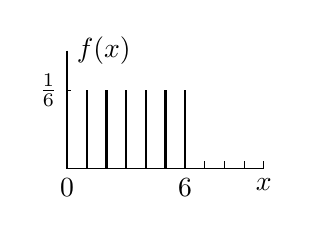
\begin{tikzpicture}[x={0.25cm}]
\draw(0,1.5)node[right]{$f(x)$}--(0,0)--(10,0)node[below]{$x$};
\foreach \x in {7,8,9,10}{\draw(\x,0)--++(0,0.1);}
\draw(0,0)node[below]{$0$} (6,0)node[below]{$6$} (0,1)node[left]{$\frac{1}{6}$}--++(0.2,0);
\foreach \x in {1,2,3,4,5,6}{\draw[thick] (\x,0)--++(0,1);}
\path(0,0)--(-2,0);
\end{tikzpicture}
\begin{tikzpicture}[x={0.25cm}]
\draw(0,3.5)--(0,0)--(10,0)node[below]{$x$};
\foreach \x in {2,3,...,10}{\draw(\x,0)--++(0,0.1);}
\foreach \x/\xx in {1/0,2/1,3/2,4/3,5/4,6/5}{\draw(\x,0.5*\xx)--++(0,0.5)node[circ]{}--++(1,0);}
\draw(7,3)--(10,3);
\foreach \y/\yy in {1.5/0.5,3/1.0}{\draw(0,\y)node[left]{$\yy$}--++(0.2,0);}
\draw(0,3.5)node[right]{$F(x)$};
\path(0,0)--(-2,0);
\end{tikzpicture}
\caption{تفاعل احتمال $f(x)$ اور تفاعل تقسیم $F(x)$}
\label{شکل_شماریات_تفاعل_تقسیم_الف}
\end{minipage}\hfill
\begin{minipage}{0.45\textwidth}
\centering
\begin{tikzpicture}[x={0.25cm}]
\draw(0,1.2)node[right]{$f(x)$}--(0,0)--(15,0)node[below]{$x$};
%\draw(0,0)node[below]{$0$} (6,0)node[below]{$6$} (0,0.5)node[left]{$\frac{1}{6}$}--++(0.2,0);
\foreach \x/\y in {2/1,3/2,4/3,5/4,6/5,7/6,8/5,9/4,10/3,11/2,12/1}{\draw[thick] (\x,0)--++(0,6*\y/36);}
\draw(5,0)node[below]{$5$};
\draw(10,0)node[below]{$10$};
\draw(0,1)node[left]{$\tfrac{1}{6}$}--++(0.2,0);
\path(0,0)--(-2,0);
\end{tikzpicture}
\begin{tikzpicture}[x={0.25cm}]
\draw(0,3.5)--(0,0)--(15,0)node[below]{$x$};
\draw(2,0)\foreach \y in {1,2,3,4,5,6,5,4,3,2,1}{--++(0,3*\y/36)node[circ]{}--++(1,0)};
\draw(13,3)--(15,3);
\draw(0,3.5)node[right]{$F(x)$};
\foreach \x in {1,2,...,15}{\draw(\x,0)--++(0,0.05);}
\draw(5,0)node[below]{$5$} (10,0)node[below]{$10$} ;
\draw(0,3)node[left]{$1$}--++(0.2,0);
\draw (0,5/6)node[left]{$\tfrac{10}{36}$}--++(0.2,0);
\draw (0,5/3)node[left]{$\tfrac{20}{36}$}--++(0.2,0);
\draw (0,5/2)node[left]{$\tfrac{30}{36}$}--++(0.2,0);
\path(0,0)--(-2,0);
\end{tikzpicture}
\caption{تفاعل احتمال $f(x)$ اور تفاعل تقسیم $F(x)$}
\label{شکل_شماریات_تفاعل_تقسیم_ب}
\end{minipage}
\end{figure}
دو پانسہ کے تجربہ میں چونکہ \عددی{6\cdot6=36} ممکنہ مساوی امکانی انجام ہیں لہٰذا ہر ایک کا احتمال \عددی{\tfrac{1}{36}} ہے۔صرف \عددی{(1,1)} کے لئے (جہاں پہلا عدد ایک پانسہ اور دوسرا عدد دوسرے پانسہ کا نتیجہ ہے) \عددی{X=2} ہو گا؛ اسی طرح \عددی{(1,2)} اور \عددی{(2,1)} انجام کے لئے \عددی{X=3} ہو گا؛ \عددی{(1,3)}، \عددی{(2,2)}، \عددی{(3,1)} کے لئے \عددی{X=4} ہو گا، وغیرہ۔

صرف وہ \عددی{x_1,x_2,x_3,\cdots} قیمتیں جن کے لئے بلا منصوبہ غیر مسلسل متغیر \عددی{X} مثبت احتمال رکھتا ہو \عددی{X} کی \اصطلاح{ممکنہ قیمتیں}\فرہنگ{ممکنہ قیمتیں}\حاشیہب{possible values}\فرہنگ{values!possible} کہلاتی ہیں۔جس وقفہ میں کوئی ممکنہ قیمت نہ پائی جاتی اس وقفہ میں تفاعل تقسیم \عددی{F(x)} مستقل ہو گا۔اس طرح \عددی{F(x)} \اصطلاح{سیڑھی تفاعل}\فرہنگ{سیڑھی تفاعل}\فرہنگ{step function} (ٹکڑوں میں مستقل تفاعل) ہو گا جس میں \عددی{x=x_j} پر اوپر رخ \عددی{p_j=P(X=x_j)} چھلانگ پائی جائے گی جبکہ دو چھلانگوں کے بیچ یہ مستقل ہو گا۔شکل \حوالہ{شکل_شماریات_تفاعل_تقسیم_الف} اور شکل \حوالہ{شکل_شماریات_تفاعل_تقسیم_ب} میں ایسا صاف ظاہر ہے۔

ہم اب استمراری بلا منصوبہ متغیر کی تعریف پیش کرتے ہیں اور اس پر غور کرتے ہیں۔ایک بلا منصوبہ متغیر \عددی{X} اور اس کا مطابقتی تفاعل تقسیم تب \اصطلاح{استمراری}\فرہنگ{استمراری}\فرہنگ{continuous} کہلاتے ہیں جب اس کا تفاعل تقسیم \عددی{F(x)=P(X\le x)} مثبت ہو اور اسے درج ذیل تکمل کی صورت میں لکھنا ممکن ہو\حاشیہد{\عددی{F(x)} استمراری ہے لیکن \عددی{F(x)} کے استمراری ہونے سے  مساوات \حوالہ{مساوات_شماریات_استمراری_بلا_منصوبہ_متغیر_الف} کی موجودگی ثابت نہیں ہوتی ہے۔چونکہ ایسے استمراری تفاعل تقسیم جنہیں مساوات \حوالہ{مساوات_شماریات_استمراری_بلا_منصوبہ_متغیر_الف} کی صورت میں لکھنا ممکن نہ ہو عملاً بہت کم پائے جاتے ہیں لہٰذا اصطلاحات "استمراری بلا منصوبہ متغیر" اور "استمراری تقسیم" جو بہت زیادہ استعمال کی جاتی ہیں سے پریشانی پیدا ہونے کا امکان بہت کم ہو گا۔}
\begin{align}\label{مساوات_شماریات_استمراری_بلا_منصوبہ_متغیر_الف}
F(x)=\int_{-\infty}^{x} f(v)\dif v
\end{align}
جہاں متکمل استمراری ہے، ماسوائے  \عددی{v} کی متناہی تعداد  کے قیمتوں کے لئے۔متکمل \عددی{f} کو تقسیم کی \ترچھا{کثافت احتمال} یا مختصراً \اصطلاح{کثافت}\فرہنگ{کثافت}\فرہنگ{density} کہتے ہیں۔ہر اس \عددی{x} پر جہاں \عددی{f(x)} استمراری ہو وہاں مساوات \حوالہ{مساوات_شماریات_استمراری_بلا_منصوبہ_متغیر_الف} کو تقسیم کرتے ہوئے 
\begin{align*}
F'(x)=f(x)
\end{align*}
حاصل ہو گا۔اس لحاظ سے تفاعل تقسیم کا تفرق کثافت ہے۔

مساوات \حوالہ{مساوات_شماریات_استمراری_بلا_منصوبہ_متغیر_الف} اور حصہ \حوالہ{حصہ_شماریات_احتمال} کے مسلمہ-ب کے تحت درج ذیل ہو گا۔
\begin{align}\label{مساوات_شماریات_استمراری_بلا_منصوبہ_متغیر_ب}
\int_{-\infty}^{\infty} f(v)\dif v=1
\end{align}
مساوات \حوالہ{مساوات_شماریات_غیر_مسلسل_متغیر_ث} اور مساوات \حوالہ{مساوات_شماریات_استمراری_بلا_منصوبہ_متغیر_الف} سے درج ذیل کلیہ حاصل ہوتا ہے۔
\begin{align}\label{مساوات_شماریات_استمراری_بلا_منصوبہ_متغیر_پ}
P(a<X\le b)=F(b)-F(a)=\int_{a}^{b}f(v)\dif v
\end{align}
یوں جیسا شکل \حوالہ{شکل_مساوات_شماریات_استمراری_بلا_منصوبہ_متغیر_پ} میں دکھایا گیا ہے، کثافت \عددی{f(x)} کے منحنی کے نیچے \عددی{x=a} اور \عددی{x=b} کے بیچ رقبہ احتمال کے برابر ہو گا۔
\begin{figure}
\centering
\begin{tikzpicture}
\draw(2,2) to [out=0,in=170]coordinate[pos=0.25](kA)coordinate[pos=0.6](kB)(4,0.25);
\draw(2,2) to [out=180,in=10]coordinate[pos=0.25](kN)(0,0.25);
\path(kA)--($(0,0)!(kA)!(4,0)$)coordinate(kD)node[below]{$a$};
\path(kB)--($(0,0)!(kB)!(4,0)$)coordinate(kC)node[below]{$b$};
\shade[gray,shading angle=180] (kA)--(kB)--(kC)--(kD)--(kA);
\draw(kA)--($(0,0)!(kA)!(4,0)$)coordinate(kD)node[below]{$a$};
\draw(kB)--($(0,0)!(kB)!(4,0)$)coordinate(kC)node[below]{$b$};
\draw(0,0)--(4,0)node[below]{$x$};
\draw[stealth-] (kN) to [out=135,in=0]++(-0.5,0.4)node[left]{$f(x)$\,\RL{کثافت}};
\draw[stealth-] ($(kC)!0.5!(kD)$)++(0,1) to [out=45,in=180]++(1,1)node[right]{$P(a<X\le b)$};
\end{tikzpicture}
\caption{شکل برائے مساوات \حوالہ{مساوات_شماریات_استمراری_بلا_منصوبہ_متغیر_پ}}
\label{شکل_مساوات_شماریات_استمراری_بلا_منصوبہ_متغیر_پ}
\end{figure}

ظاہر ہے کہ کسی بھی  مقررہ \عددی{a} اور \عددی{b\,(>a)} کے لئے وقفہ \عددی{a<X\le b}، \عددی{a<X<b} اور \عددی{a\le X<b} کے احتمال ایک جیسے ہوں گے جو غیر مسلسل صورت حال سے مختلف ہے۔

استمراری تقسیم کے مثال (سوالات) اگلے حصے کے سوالات اور آنے والے حصوں میں پیش کئے جائیں گے۔

%=====================
\حصہء{سوالات}
%=============
\ابتدا{سوال}\quad
تفاعل احتمال \عددی{f(x)=\tfrac{x^2}{14}\,\, (x=1,2,3)} اور تفاعل تقسیم کی ترسیم کھینچیں۔
\انتہا{سوال}
%====================
\ابتدا{سوال}\quad
\عددی{X} کا تفاعل احتمال \عددی{f(2)=\tfrac{1}{2}}، \عددی{f(3)=\tfrac{1}{4}}، \عددی{f(4)=f(5)=\tfrac{1}{8}} ہے۔اس کا کیا احتمال ہے کہ \عددی{X} کی قیمت \عددی{4} سے کم ہو گی؟
\انتہا{سوال}
%=====================
\ابتدا{سوال}\quad
ایک مشین کو \عددی{X} سالوں کے بعد تبدیل کرنا ضروری ہے۔\عددی{X} کا تفاعل احتمال \عددی{f(1)=0.3}، \عددی{f(2)=0.4}، \عددی{f(3)=0.2}، \عددی{f(4)=0.1} ہے۔\عددی{f} اور \عددی{F} کو ترسیم کریں۔
\انتہا{سوال}
%====================
\ابتدا{سوال}\quad
کسی پٹرول پمپ میں ایک دن کی درکار پٹرول بلا منصوبہ متغیر \عددی{X} ہے۔ فرض کریں کہ \عددی{2000<x<6000} کے لئے \عددی{X} کی کثافت \عددی{f(x)=k} ہے ورنہ \عددی{0} ہے۔\عددی{k} تلاش کریں اور تفاعل تقسیم \عددی{F(x)} ترسیم کریں۔\\
جواب:\quad
\begin{align*}
k=\tfrac{1}{4000},\quad 
F(x)=
\begin{cases}
0&x<2000\\
\tfrac{x}{4000}-0.5&2000\le x<6000\\
1&x\ge 6000
\end{cases}
\end{align*}
\انتہا{سوال}
%==========================
\ابتدا{سوال}\quad
\عددی{x>0} کے لئے \عددی{f(x)=ce^{-x}} جبکہ \عددی{x<0} کے لئے \عددی{f(x)=0} ہے۔\عددی{c} تلاش کریں۔ \عددی{f} اور \عددی{F} کر ترسیم کریں۔
\انتہا{سوال}
%=======================
\ابتدا{سوال}\quad
\عددی{3} پانسہ اچھال کر ان کا مجموعہ لے کر بلا منصوبہ متغیر \عددی{X} حاصل کیا جاتا ہے۔تفاعل احتمال \عددی{f(x)} ترسیم کریں۔\\
جواب:\quad
$f(3)=\tfrac{1}{216}, f(4)=\tfrac{3}{216},\cdots$
\انتہا{سوال}
%======================
\ابتدا{سوال}\quad
کاغذ کے گتے کی موٹائی \عددی{X} ملی میٹر ہے۔ فرض کریں کہ \عددی{1.9<x<2.1} کے لئے کثافت \عددی{f(x)=kx} ہے ورنہ \عددی{f(x)=0} ہے۔\عددی{k} تلاش کریں۔اس کا کیا احتمال ہے کہ گتے کی موٹائی \عددی{1.95} اور \عددی{2.05} کے بیچ ہو؟
\انتہا{سوال}
%=================
\ابتدا{سوال}\quad
ایک سکہ کو اتنی مرتبہ (\عددی{X})  اچھالا جاتا ہے جب تک خط حاصل نہ ہو۔دکھائیں کہ اس تجربہ کا تفاعل احتمال \عددی{f(x)=2^{-x},\,\, (x=1,2,\cdots)} ہو گا۔دکھائیں کہ \عددی{f(x)} مساوات \حوالہ{مساوات_شماریات_غیر_مسلسل_متغیر_پ} کو مطمئن کرتا ہے۔
\انتہا{سوال}
%=======================
\ابتدا{سوال}\quad
\عددی{0\le x\le 1} کے لئے \عددی{f(x)=kx^2} ہے ورنہ \عددی{f(x)=0} ہے۔\عددی{k} تلاش کریں۔ایسا عدد \عددی{c} تلاش کریں کہ \عددی{P(X\le c)=\SI{72.9}{\percent}} ہو۔
\انتہا{سوال}
%=======================
\ابتدا{سوال}\quad
بلب کی عرصہ زندگی \عددی{X} بلا منصوبہ متغیر ہے جس کی کثافت
\begin{align*}
f(x)=6[0.25-(x-1.5)^2]\quad \quad 1\le x\le 2
\end{align*}
 اور باقی \عددی{x} کے لئے \عددی{f(x)=0} ہے، جہاں \عددی{x=1} سے مراد \عددی{1000} گھنٹے ہیں۔ کیا احتمال ہے کہ سڑک کے اشارے پر پہلے \عددی{1200} گھنٹوں میں تین میں سے کسی ایک بھی بلب کی تبدیل کرنے کی ضرورت پیش نہ آئے؟\\
جواب:\quad
$P(X>1200)=\int_{1.2}^{2}6[0.25-(x-1.5)^2]\dif x=0.896^3=\SI{72}{\percent}$
\انتہا{سوال}
%========================
\ابتدا{سوال}\quad
کسی دکان کی فروخت اور منافع کی نسبت  \عددی{X} ہے۔ فرض کریں کہ \عددی{X} کی تفاعل تقسیم \عددی{x<2} کے لئے \عددی{F(x)=0}، \عددی{2\le x<3} کے لئے \عددی{F(x)=\tfrac{x^2-4}{5}} اور \عددی{x\ge 3} کے لئے \عددی{F(x)=1} ہے۔کثافت تلاش کر کے ترسیم کریں۔\عددی{X} کی  قیمت \عددی{2.5} (\عددی{\SI{40}{\percent}} منافع) اور \عددی{5} (\عددی{\SI{20}{\percent}} منافع) کے بیچ میں ہونے کا کیا احتمال ہے؟  
\انتہا{سوال}
%========================
\ابتدا{سوال}\quad
\عددی{X} ایک بلا منصوبہ متغیر ہے جو کوئی بھی حقیقی قیمت اختیار کر سکتا ہے۔وقوعہ \عددی{X\le b}، \عددی{X<b}، \عددی{X\ge c}، \عددی{X>c}، \عددی{b\le X\le c}، \عددی{b<X\le x} کے متمم کے کیا احتمال ہوں گے؟\\
جواب:\quad
$X\le b \,\text{یا} \,X>c,X<b \,\text{یا} \, X>c,X\le c,X<c,X\ge b,X>b$
\انتہا{سوال}
%=========================
\ابتدا{سوال}\quad
ایک ڈبہ میں \عددی{4} دائیں ہاتھ پیچ اور \عددی{6} بائیں ہاتھ پیچ پائے جاتے ہیں۔بغیر واپس رکھے، دو پیچ بلا منصوبہ نکالے جاتے ہیں۔نکالے گئے بائیں ہاتھ پیچوں کی تعداد \عددی{X} ہے۔ احتمال \عددی{P(X=0)}، \عددی{P(X=1)}، \عددی{P(1<X<2)} \عددی{P(X\le 1)}، \عددی{P(X\ge 1)}، \عددی{P(X>1)}،\عددی{P(0.5<X<10)} تلاش کریں۔
\انتہا{سوال}
%===========================
\ابتدا{سوال}\quad
دکھائیں کہ \عددی{b<c} سے مراد \عددی{P(X\le b)\le P(X\le c)} ہے۔
\انتہا{سوال}
%============================

\حصہ{تقسیم کا اوسط اور  اس کی تغیریت}\شناخت{حصہ_شماریات_تقسیم_کا_اوسط_اور_تغیریت}
\ترچھا{تقسیم} کے \اصطلاح{اوسط}\فرہنگ{اوسط}\حاشیہب{mean}\فرہنگ{mean} کو \عددی{\mu} سے ظاہر کیا جاتا ہے اور اس کی تعریف درج ذیل ہے۔
\begin{gather}
\begin{aligned}\label{مساوات_شماریات_اوسط_تغیریت_الف}
\text{(الف)}\quad\mu&=\sum_{j} x_jf(x_j)\quad\quad \quad (\text{\RL{غیر مسلسل تقسیم}})\\
\text{(ب)}\quad \mu&=\int_{-\infty}^{\infty} xf(x)\dif x\quad\quad\quad (\text{\RL{استمراری تقسیم}})
\end{aligned}
\end{gather}
مساوات \حوالہ{مساوات_شماریات_اوسط_تغیریت_الف}-الف میں زیر غور بلا منصوبہ متغیر \عددی{X} کا تفاعل احتمال \عددی{f(x)} ہے اور ہم تمام ممکنہ قیمتوں (حصہ \حوالہ{حصہ_شماریات_بلا_منصوبہ_متغیرات}) پر مجموعہ لیتے ہیں۔مساوات \حوالہ{مساوات_شماریات_اوسط_تغیریت_الف}-ب میں \عددی{X} کی کثافت \عددی{f(x)} ہے۔اوسط کو \عددی{X} کی \اصطلاح{حسابی توقع}\فرہنگ{حسابی!توقع}\حاشیہب{mathematical expectation}\فرہنگ{expectation!mathematical} بھی کہتے ہیں جس کو \عددی{E(X)} سے ظاہر کیا جاتا ہے۔تعریف کی رو سے ہم فرض کرتے ہیں کہ مساوات \حوالہ{مساوات_شماریات_اوسط_تغیریت_الف}-الف کی تسلسل مطلق مرتکز ہو گی اور \عددی{-\infty} سے \عددی{\infty} تک \عددی{\abs{x}f(x)} کا تکمل موجود ہو گا۔اگر یہ تکمل موجود نہ ہو تب ہم کہتے ہیں کہ اس تقسیم کی اوسط نہیں ہائی جاتی ہے؛ ایسی صورت عملی انجینئری میں شاذ و نادر پائی جاتی ہے۔  

\عددی{x=c} کے لحاظ سے ایک تقسیم کو اس صورت تشاکلی کہتے ہیں جب ہر حقیقی \عددی{x} کے لئے درج ذیل مطمئن ہوتا ہو۔
\begin{align}\label{مساوات_شماریات_اوسط_تغیریت_ب}
f(c+x)=f(c-x)
\end{align} 
آپ درج ذیل مسئلہ ثابت کر سکتے ہیں (سوال \حوالہ{سوال_شماریات_اوسط_الف})۔

%===============
\ابتدا{مسئلہ}\شناخت{مسئلہ_شماریات_تشاکلی_تقسیم_کا_اوسط}\quad \موٹا{(تشاکلی تقسیم کا اوسط)}\\
اگر ایک تقسیم \عددی{x=c} کے لحاظ سے تشاکلی ہو اور اس کا اوسط \عددی{\mu} ہو تب \عددی{\mu=c} ہو گا۔ 
\انتہا{مسئلہ}
%=========================

تقسیم کی \اصطلاح{تغیریت}\فرہنگ{تغیریت}\حاشیہب{variance}\فرہنگ{variance} کو \عددی{\sigma^{\,2}} سے ظاہر کیا جاتا ہے اور اس کی تعریف درج ذیل کلیہ دیتی ہے
\begin{gather}
\begin{aligned}\label{مساوات_شماریات_اوسط_تغیریت_پ}
\text{(الف)}\quad \sigma^{\,2}&=\sum_{j} (x_j-\mu)^2f(x_j)\quad\quad\quad (\text{\RL{غیر مسلسل تقسیم}})\\
\text{(ب)}\quad \sigma^{\,2}&=\int_{-\infty}^{\infty} (x-\mu)^2f(x)\dif x\quad \quad \quad (\text{\RL{استمراری تقسیم}})
\end{aligned}
\end{gather}
جہاں تعریف کی رو سے ہم فرض کرتے ہیں کہ مساوات \حوالہ{مساوات_شماریات_اوسط_تغیریت_پ}-الف میں دی گئی تسلسل مطلق مرتکز ہے اور مساوات \حوالہ{مساوات_شماریات_اوسط_تغیریت_پ}-ب کا تکمل موجود ہے۔

غیر مسلسل تقسیم کی صورت میں اگر کسی ایک نقطہ پر \عددی{f(x)=1} اور باقی ہر جگہ \عددی{f(x)=0} ہو تب \عددی{\sigma^2=0} ہو گا جو عملاً غیر دلچسپ صورت ہے۔اس غیر دلچسپ صورت  کے علاوہ ہر صورت میں درج ذیل ہو گا۔
\begin{align}\label{مساوات_شماریات_اوسط_تغیریت_ت}
\sigma^{\,2}>0
\end{align}

تغیریت کا مثبت جذر \اصطلاح{معیاری انحراف}\فرہنگ{معیاری انحراف}\فرہنگ{انحراف!معیاری}\حاشیہب{standard deviation}\فرہنگ{standard deviation} کہلاتا ہے جس کو \عددی{\sigma} سے ظاہر کیا جاتا ہے۔ 

بلا منصوبہ متغیر \عددی{X} جن قیمتوں کو اختیار کر سکتا ہے، تغیریت کو ان قیمتوں کی پھیل کی ناپ تصور کیا جا سکتا ہے۔ 

%=================
\ابتدا{مثال}\quad \موٹا{(اوسط اور تغیریت)}\\
بلا منصوبہ متغیر
\begin{align*}
X=\text{\RL{سکہ اچھال کر شیر کا حاصل ہونا}}
\end{align*}
کے ممکنہ قیمتیں \عددی{X=0} اور \عددی{X=1} ہیں جن کا احتمال \عددی{P(X=0)=\tfrac{1}{2}} اور \عددی{P(X=1)=\tfrac{1}{2}} ہے۔مساوات \حوالہ{مساوات_شماریات_اوسط_تغیریت_الف}-الف سے اوسط \عددی{\mu=0\cdot \tfrac{1}{2}+1\cdot\tfrac{1}{2}=\tfrac{1}{2}} حاصل ہوتا ہے۔مساوات \حوالہ{مساوات_شماریات_اوسط_تغیریت_الف}-ب سے درج ذیل حاصل ہو گا۔
\begin{align*}
\sigma^{\,2}=(0-\tfrac{1}{2})^2\cdot \tfrac{1}{2}+(1-\tfrac{1}{2})^2\cdot \tfrac{1}{2}=\tfrac{1}{4}
\end{align*}
\انتہا{مثال}
%=======================
\ابتدا{مثال}\quad \موٹا{یکساں تقسیم}\\
وہ تقسیم جس کی کثافت \عددی{a<x<b} کے لئے
\begin{align*}
f(x)=\frac{1}{b-a}\quad \quad (a<x<b\,\,\text{جب})
\end{align*}
اور باقی \عددی{x} کے لئے \عددی{f=0} ہو، وقفہ \عددی{a<x<b} میں \اصطلاح{یکساں تقسیم}\فرہنگ{تقسیم!یکساں}\حاشیہب{uniform distribution}\فرہنگ{distribution!uniform} کہلاتی ہے۔ مسئلہ \حوالہ{مسئلہ_شماریات_تشاکلی_تقسیم_کا_اوسط} یا مساوات \حوالہ{مساوات_شماریات_اوسط_تغیریت_پ}-الف سے \عددی{\mu=\tfrac{a+b}{2}} اور مساوات \حوالہ{مساوات_شماریات_اوسط_تغیریت_پ}-ب سے  تغیریت حاصل کرتے ہیں۔
\begin{align*}
\sigma^{\,2}=\int_a^b (x-\tfrac{a+b}{2})^2\tfrac{1}{b-a}\dif x=\frac{(b-a)^2}{12}
\end{align*}
شکل \حوالہ{شکل_شماریات_یکساں_تقسیم_اوسط_تغیریت} میں چند خصوصی مثالیں پیش کی گئی ہیں جو دکھاتی ہیں کہ \عددی{\sigma^{\,2}} پھیل کی ناپ ہے۔ 
\انتہا{مثال}
%===========================
\begin{figure}
\centering
\begin{subfigure}{0.5\textwidth}
\centering
\begin{tikzpicture}
\draw(-0.5,0)--(1.5,0)node[right]{$x$};
\draw(0,0)--(0,1.5)node[right]{$f(x)$};
\draw[thick] (-0.5,0)--(0,0)node[below]{$0$}--(0,1)node[left]{$1$}--(1,1)--(1,0)node[below]{$1$}--(1.5,0);
\draw(1,1)node[above right]{$(\sigma^{\,2}=\tfrac{1}{12})$};
\path(3,0)--(3.5,0);
\end{tikzpicture}
\end{subfigure}%
\begin{subfigure}{0.5\textwidth}
\centering
\begin{tikzpicture}
\draw(-1.5,0)--(2.5,0)node[right]{$x$};
\draw(0,0)node[below]{$0$}--(0,1.5)node[right]{$f(x)$};
\draw[thick](-1.5,0)--(-1,0)node[below]{$-1$}--(-1,1/3)--(2,1/3)--(2,0)node[below]{$2$}--(2.5,0);
\draw(0,1)node[left]{$1$}--++(0.2,0);
\draw(1,1)node[above right]{$(\sigma^{\,2}=\tfrac{3}{4})$};
\end{tikzpicture}
\end{subfigure}
\begin{subfigure}{0.5\textwidth}
\centering
\begin{tikzpicture}
\draw(0,0)--(0,1.5)node[right]{$F(x)$};
\draw(-0.5,0)--(1.5,0)node[right]{$x$};
\draw[thick](-0.5,0)--(0,0)--(1,1)--(1.5,1);
\draw(1,0)node[below]{$1$}--++(0,0.2);
\draw(0,1)node[left]{$1$}--++(0.2,0);
\path(3,0)--(3.5,0);
\end{tikzpicture}
\end{subfigure}%
\begin{subfigure}{0.5\textwidth}
\centering
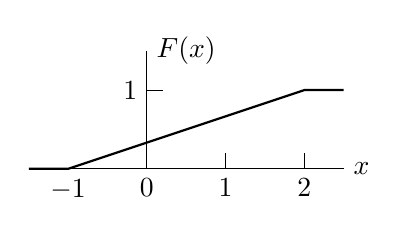
\begin{tikzpicture}
\draw(-1.5,0)--(2.5,0)node[right]{$x$};
\draw(0,0)node[below]{$0$}--(0,1.5)node[right]{$F(x)$};
\draw[thick](-1.5,0)--(-1,0)node[below]{$-1$}--(2,1)--(2.5,1);
\draw(1,0)node[below]{$1$}--++(0,0.2);
\draw(2,0)node[below]{$2$}--++(0,0.2);
\draw(0,1)node[left]{$1$}--++(0.2,0);
\end{tikzpicture}
\end{subfigure}%
\caption{یکساں تقسیم جن کی ایک جیسی اوسط \عددی{(0.5)} لیکن مختلف تغیریت \عددی{\sigma^{\,2}} ہے}
\label{شکل_شماریات_یکساں_تقسیم_اوسط_تغیریت}
\end{figure}

%==================
\ابتدا{مسئلہ}\شناخت{مسئلہ_شماریات_خطی_تبادل}\quad \موٹا{(خطی تبادل)}\\
اگر بلا منصوبہ متغیر \عددی{X} کی اوسط \عددی{\mu} اور تغیریت \عددی{\sigma^{\,2}} ہو تب بلا منصوبہ متغیر \عددی{X^*=c_1X+c_2\,(c_1\ne 0)} کی اوسط
\begin{align}\label{مساوات_شماریات_اوسط_تغیریت_ٹ}
\mu^*=c_1\mu+c_2
\end{align}
 اور تغیریت
\begin{align}\label{مساوات_شماریات_اوسط_تغیریت_ث}
\sigma^{*2}=c_1^{\,2}\sigma^{\,2}
\end{align}
ہو گی۔
\انتہا{مسئلہ}
%=======================
\ابتدا{ثبوت}\quad
ہم پہلے \عددی{c_1>0} فرض کرتے ہوئے مساوات \حوالہ{مساوات_شماریات_اوسط_تغیریت_ٹ} کو استمراری صورت کے لئے ثابت کرتے ہیں۔چونکہ \عددی{X} محور پر چھوٹے سے وقفہ \عددی{\Delta x} کا مطابقتی احتمال (تخمیناً) \عددی{f(x)\Delta x} ہو گا جو ہر صورت \عددی{X^*} محور پر مطابقتی چھوٹے وقفہ \عددی{\Delta x^*=c_1\Delta x} پر احتمال \عددی{f^*(x^*)\Delta x^*} کے برابر ہو گا لہٰذا \عددی{x} اور \عددی{x^*=c_1x+c_2} کے مطابقتی، \عددی{X} کی کثافت \عددی{f(x)} اور \عددی{X^*} کی کثافت \عددی{f^*(x^*)}،  تعلق \عددی{f^*(x^*)=\tfrac{f(x)}{c_1}} کو مطمئن کریں گے۔چونکہ \عددی{\tfrac{\dif x^*}{\dif x}=c_1} ہے لہٰذا \عددی{\dif x^*=c_1\dif x} اور \عددی{f^*(x^*)\dif x^*=f(x)\dif x} ہو گا۔یوں درج ذیل ہو گا
\begin{align*}
\mu^*=\int_{-\infty}^{\infty} x^*f^*(x^*)\dif x^*&=\int_{-\infty}^{\infty} (c_1x+c_2)f(x)\dif x\\
&=c_1\int_{-\infty}^{\infty}xf(x)\dif x+c_2\int_{-\infty}^{\infty}f(x)\dif x
\end{align*}
جہاں آخری تکمل مساوات \حوالہ{مساوات_شماریات_استمراری_بلا_منصوبہ_متغیر_ب} کے تحت \عددی{1} کے برابر ہو گا۔یوں  مساوات \حوالہ{مساوات_شماریات_اوسط_تغیریت_ٹ} ثابت ہوتی ہے۔چونکہ
\begin{align*}
x^*-\mu^*=(c_1x+c_2)-(c_1\mu+c_2)=c_1x-c_1\mu
\end{align*}
ہے لہٰذا تغیریت کی تعریف سے
\begin{align*}
\sigma^{*2}=\int_{-\infty}^{\infty} (x^*-\mu^*)^2f^*(x^*)\dif x^*=\int_{-\infty}^{\infty} (c_1x-c_1\mu)^2f(x)\dif x=c_1^2\sigma^2
\end{align*}
حاصل ہو گا۔ \عددی{c_1<0} سے نتائج تبدیل نہیں ہوتے ہیں چونکہ اس سے دو اضافی منفی کی علامتیں ملتی ہیں، ایک \عددی{x} میں تکمل کے رخ کی تبدیلی کی بنا (دھیان رہے کہ \عددی{x^*=-\infty} کا مطابقتی \عددی{x=\infty} ہے) اور دوسرا \عددی{f^*(x^*)=\tfrac{f(x)}{-c_1}} کی بنا؛ یہاں \عددی{-c_1>0} درکار ہو گا چونکہ کثافت غیر منفی قیمت ہے۔  

غیر مسلسل کثافت کے لئے مسئلے کا ثبوت بھی بالکل ایسا ہی ہے۔ 
\انتہا{ثبوت}
%========================

مساوات \حوالہ{مساوات_شماریات_اوسط_تغیریت_ٹ} اور مساوات \حوالہ{مساوات_شماریات_اوسط_تغیریت_ث} سے ہم درج ذیل اخذ کر سکتے ہیں۔

%=========================
\ابتدا{مسئلہ}\شناخت{مسئلہ_شماریات_معیاری_متغیر}\quad \موٹا{(معیاری متغیر)}\\
اگر بلا منصوبہ متغیر \عددی{X} کی اوسط \عددی{\mu} اور تغیریت \عددی{\sigma^2} ہو، تب مطابقتی متغیر \عددی{Z=\tfrac{X-\mu}{\sigma}} کی اوسط \عددی{0} اور تغیریت \عددی{1} ہو گی۔
\انتہا{مسئلہ}
%==============================

\عددی{Z} کو \عددی{X} کا مطابقتی \اصطلاح{معیاری متغیر}\فرہنگ{معیاری!متغیر}\حاشیہب{standardized variable}\فرہنگ{variable!standardized} کہتے ہیں۔

اگر \عددی{X} کوئی بلا منصوبہ متغیر اور \عددی{g(X)} کوئی استمراری تفاعل ہو جو تمام حقیقی \عددی{X} کے لئے معین ہو تب عدد
\begin{gather}
\begin{aligned}\label{مساوات_شماریات_اوسط_تغیریت_ج}
\text{(الف)}\quad E(g(X))&=\sum_j g(x_j)f(x_j)\quad\quad (X\,\text{\RL{غیر مسلسل}})\\
\text{(ب)}\quad E(g(X))&=\int_{-\infty}^{\infty} g(x)f(x)\dif x\quad\quad (X\,\text{\RL{استمرای}}) 
\end{aligned}
\end{gather}
کو \عددی{g(X)} کی \اصطلاح{حسابی توقع}\فرہنگ{توقع!حسابی}\حاشیہب{mathematical expectation}\فرہنگ{expectation!mathematical} کہتے ہیں۔ یہاں \عددی{f} بالترتیب تفاعل احتمال یا کثافت ہے۔

مساوات \حوالہ{مساوات_شماریات_اوسط_تغیریت_ج} میں \عددی{g(X)=X^k\,\, (k=1,2,\cdots)} لیتے ہوئے بالترتیب 
\begin{align}
E(X^k)=\int_{-\infty}^{\infty} x^kf(x)\dif x\quad \text{اور}\quad E(X^k)=\sum_j x_j^k f(x_j)
\end{align}
حاصل ہوتے ہیں۔ \عددی{E(X^k)} کو \عددی{X} کا \اصطلاح{\عددی{k} واں معیار اثر}\فرہنگ{معیار اثر}\حاشیہب{kth moment}\فرہنگ{moment!k} کہتے ہیں۔مساوات \حوالہ{مساوات_شماریات_اوسط_تغیریت_ج} میں \عددی{g(X)=(X-\mu)^k} لیتے ہوئے بالترتیب
\begin{align}
E([X-\mu]^k)=\int_{-\infty}^{\infty} (x-\mu)^kf(x)\dif x\quad \text{اور}\quad E([X-\mu]^k)=\sum_j(x_j-\mu)^kf(x_j)
\end{align}
حاصل ہوتے ہیں  جنہیں \عددی{X} کے \اصطلاح{\عددی{k} ویں وسطی معیار اثر}\فرہنگ{معیار اثر!وسطی}\حاشیہب{kth central moment}\فرہنگ{moment!central, kth} کہتے ہیں۔آپ درج ذیل ثابت کر سکتے ہیں۔
\begin{align}
E(1)&=1\label{مساوات_شماریات_وسطی_معیار_اثر_الف}\\
\mu&=E(X)\label{مساوات_شماریات_وسطی_معیار_اثر_ب}\\
\sigma^2&=E([X-\mu]^2)\label{مساوات_شماریات_وسطی_معیار_اثر_پ}
\end{align}

%=================
\حصہء{سوالات}

%======================
\ابتدا{سوال}\شناخت{سوال_شماریات_اوسط_الف}\quad
مسئلہ \حوالہ{مسئلہ_شماریات_تشاکلی_تقسیم_کا_اوسط} ثابت کریں۔\\
جواب:\quad
\begin{align*}
&\mu=\int_{-\infty}^{c} tf(t)\dif t+\int_{c}^{\infty}tf(t)\dif t\\
&=-\int_{\infty}^{0}(c-x)f(c-x)\dif x+\int_{0}^{\infty}(c+x)f(c+x)\dif x=2c\int_{0}^{\infty}f(c+x)\dif x=c
\end{align*}
غیر مسلسل تقسیم کے لئے بھی ثبوت اسی طرح حاصل کیا جا سکتا ہے۔
\انتہا{سوال}
%===================
\ابتدا{سوال}\quad
ایک تقسیم کی کثافت  \عددی{f(x)=\tfrac{1}{2}e^{-\abs{x}}} ہے۔اس  کی اوسط اور تغیریت تلاش کریں۔\\
جواب:\quad
$\mu=0,\sigma^2=2$
\انتہا{سوال}
%======================
\ابتدا{سوال}\شناخت{سوال_شماریات_اوسط_پ}\quad
\عددی{0\le x\le 2} کے لئے \عددی{X} کی کثافت \عددی{f(x)=0.5x} ہے جبکہ باقی \عددی{x} کے لئے \عددی{f(x)=0} ہے۔دکھائیں کہ \عددی{X} کی اوسط \عددی{\tfrac{4}{3}} اور تغیریت \عددی{\tfrac{2}{9}} ہے۔
\انتہا{سوال}
%==========================
\ابتدا{سوال}\quad
\عددی{Y=-2X+5} کی اوسط اور تغیریت تلاش کریں۔ بلا منصوبہ متغیر \عددی{X} سوال \حوالہ{سوال_شماریات_اوسط_پ} میں دیا گیا ہے۔
\انتہا{سوال}
%============================
\ابتدا{سوال}\quad
سوال \حوالہ{سوال_شماریات_اوسط_پ} کے \عددی{X} کا مطابقتی معیاری بلا منصوبہ متغیر  تلاش کریں۔\\
جواب:\quad
$\tfrac{X-\tfrac{4}{3}}{\sqrt{\tfrac{2}{9}}}$
\انتہا{سوال}
%===========================
\ابتدا{سوال}\quad
مسئلہ \حوالہ{مسئلہ_شماریات_خطی_تبادل} کو غیر مسلسل صورت کے لئے ثابت کریں۔
\انتہا{سوال}
%============================
\ابتدا{سوال}\quad
مسئلہ \حوالہ{مسئلہ_شماریات_معیاری_متغیر} کو مساوات \حوالہ{مساوات_شماریات_اوسط_تغیریت_ٹ} اور مساوات \حوالہ{مساوات_شماریات_اوسط_تغیریت_ث} سے اخذ کریں۔\\
جواب:\quad مساوات \حوالہ{مساوات_شماریات_اوسط_تغیریت_ٹ} اور مساوات \حوالہ{مساوات_شماریات_اوسط_تغیریت_ث} میں \عددی{c_1=\tfrac{1}{\sigma}} اور \عددی{c_2=-\tfrac{\mu}{\sigma}} پر کریں۔
\انتہا{سوال}
%=========================
\ابتدا{سوال}\quad
ایک مخصوص قسم کے ٹائر بلا منصوبہ متغیر \عددی{X} (ہزار کلو میٹر) چلتے ہیں۔\عددی{X} کی کثافت \عددی{x>0} کے لئے \عددی{f(x)=\theta e^{-\theta x}} ورنہ \عددی{0} ہے جہاں \عددی{\theta\,(>0)} مقدار معلوم ہے۔ (الف) ایسے ایک ٹائر سے کتنے کلومیٹر طے کیے جا سکتے ہیں؟ (ب) اگر \عددی{\theta=0.05} ہو تب کم سے کم \عددی{\num{30000}} کلومیٹر تک پہنچنے کا احتمال کیا ہو گا؟
\انتہا{سوال}
%==========================
\ابتدا{سوال}\شناخت{سوال_شماریات_کیل_پیداوار_الف}\quad
ایک کارخانے میں کیل بنائے جاتے ہیں جن کا وتر \عددی{X} سنٹی میٹر ہے۔فرض کریں کہ \عددی{X} کی کثافت \عددی{0.9<x<1.1} کے لئے \عددی{f(x)=k(x-0.9)(1.1-x)} ورنہ \عددی{0} ہے۔\عددی{k} معلوم کریں، \عددی{f(x)} کو ترسیم کریں اور \عددی{\mu} اور \عددی{\sigma^2} کو تلاش کریں۔ \\
جواب:\quad
$k=750,\mu=1,\sigma^2=0.002$
\انتہا{سوال}
%========================
\ابتدا{سوال}\quad
سوال \حوالہ{سوال_شماریات_کیل_پیداوار_الف} میں اگر کیل کے وتر کا \عددی{\SI{1}{\centi\meter}} سے انحراف \عددی{\SI{0.06}{\centi\meter}} بڑھ جائے تب اس کو عیب دار تصور کیا جاتا ہے۔کتنے فی صد کیل عیب دار ہوں گے؟
\انتہا{سوال}
%=============================
\ابتدا{سوال}\شناخت{سوال_شماریات_پٹرول_پمپ_الف}\quad
ایک پٹرول پمپ کو ہر جمعرات دوپہر کے وقت  پٹرول مہیا کیا جاتا ہے۔فروخت پٹرول کا حجم \عددی{X} ہزار لٹر ہے۔ \عددی{0\le x\le 1} کے لئے \عددی{X} کی کثافت احتمال \عددی{f(x)=6x(1-x)} ورنہ \عددی{0} ہے۔ اوسط اور تغیریت تلاش کریں۔\\
جواب:\quad
$\mu=\tfrac{1}{2},\,\sigma^2=\tfrac{1}{20}$
\انتہا{سوال}
%==============================
\ابتدا{سوال}\quad
سوال \حوالہ{سوال_شماریات_پٹرول_پمپ_الف}  میں پٹرول کی ٹینکی کا حجم کتنا ہو گا اگر ایک ہفتہ میں ٹینکی خالی ہونے کا احتمال \عددی{\SI{10}{\percent}} ہو؟
\انتہا{سوال}
%===========================
\ابتدا{سوال}\quad
مساوات \حوالہ{مساوات_شماریات_وسطی_معیار_اثر_الف}، مساوات \حوالہ{مساوات_شماریات_وسطی_معیار_اثر_ب} اور مساوات \حوالہ{مساوات_شماریات_وسطی_معیار_اثر_پ} ثابت کریں۔
\انتہا{سوال}
%===========================
\ابتدا{سوال}\شناخت{سوال_شماریات_تغیریت_دوسرا_کلیہ}\quad
دکھائیں کہ \عددی{E(X-\mu)=0} اور \عددی{\sigma^{\,2}=E(X^2)-\mu^2} ہوں گے۔
\انتہا{سوال}
%============================
\ابتدا{سوال}\quad
فرض کریں کہ \عددی{X} کی کثافت \عددی{0<x<1} کے لئے \عددی{f(x)=2x} ورنہ \عددی{0} ہے۔ تمام معیار اثر تلاش کریں۔سوال \حوالہ{سوال_شماریات_تغیریت_دوسرا_کلیہ} میں دیے گئے کلیہ سے \عددی{\sigma^{\,2}} حاصل کریں۔\\
جواب:\quad
$E(X^k)=\tfrac{2}{k+2},\,\,\sigma^{\,2}=\tfrac{1}{18}$
\انتہا{سوال}
%============================
\ابتدا{سوال}\شناخت{سوال_شماریات_خطی_مجموعہ_کلیہ}\quad
دکھائیں کہ \عددی{E(ag(X)+bh(X))=aE(g(X))+bE(h(X))} ہو گا جہاں \عددی{a} اور \عددی{b} مستقل ہیں۔
\انتہا{سوال}
%========================
\ابتدا{سوال}\quad
وقفہ \عددی{0\le x\le 1} پر یکساں تقسیم کے معیار اثر تلاش کریں۔\\
جواب:\quad
$E(X^k)=\tfrac{1}{k+1}$
\انتہا{سوال}
%==========================
\ابتدا{سوال}\quad \موٹا{(ترچھاپن)} \quad
عدد \عددی{\gamma=\tfrac{1}{\sigma^3}E([X-\mu]^3)} کو \عددی{X} کا \اصطلاح{ترچھاپن}\فرہنگ{ترچھاپن}\حاشیہب{skewness}\فرہنگ{skewness} کہتے ہیں۔اس اصطلاح کا جواز پیش کرنے کی خاطر دکھائیں کہ \عددی{\mu} کے لحاظ سے تشاکلی \عددی{X} کے لئے اگر تیسرا وسطی معیار اثر موجود ہو تب یہ معیار اثر صفر ہو گا۔ 
\انتہا{سوال}
%==============================
\ابتدا{سوال}\quad
\عددی{x>0} کے لئے کثافت تقسیم  \عددی{f(x)=xe^{-x}} ورنہ \عددی{f=0} کی صورت میں کثافت تقسیم کا ترچھاپن تلاش کریں۔\عددی{f(x)} کو ترسیم کریں۔\\
جواب:\quad 
تکمل بالحصص لیں\quad
$\sigma^{\,2}=2,\gamma=\tfrac{4}{2\sqrt{2}}=\sqrt{2}$
\انتہا{سوال}
%========================================
\ابتدا{سوال}\شناخت{سوال_شماریات_معیار_اثر_پیدا_کار_تفاعل_الف}\quad \موٹا{(معیار اثر کا پیدا کار تفاعل)}\\
بلا منصوبہ غیر مسلسل یا استمراری متغیر \عددی{X} کے معیار اثر کا پیدا کار تفاعل درج ذیل کلیات دیتے ہیں
\begin{align*}
G(t)=E(e^{tX})=\sum_j e^{tx_j}f(x_j)\quad \text{اور}\quad G(t)=E(e^{tX})=\int_{-\infty}^{\infty} e^{tx}f(x)\dif x
\end{align*} 
جہاں فرض کیا گیا ہے کہ مجموعہ کی علامت کے اندر اور تکمل کی علامت کے اندر تفرق لیا جا سکتا ہے۔دکھائیں کہ \عددی{E(X^k)=G^{(k)}(0)} ہو گا اور بالخصوص \عددی{\mu=G'(0)} ہو گا جہاں \عددی{G^{(k)}(t)} سے مراد \عددی{t} کے لحاظ سے \عددی{G} کا \عددی{k} واں تفرق ہے۔
\انتہا{سوال}
%==============================

\حصہ{ثنائی، پوئسن، اور بیش ہندسی تقسیم}\شناخت{حصہ_شماریات_ثنائی_پوئسن_بیش_ہندسی_تقسیم}
ہم اب چند مخصوص غیر مسلسل تقسیم پر غور کرتے ہیں جو شماریات کے لئے اہم ہیں۔

\جزوحصہء{ثنائی تقسیم}
ہم ایک تجربہ کو \عددی{n} مرتبہ بلا منصوبہ سرانجام دینے میں وقوعہ \عددی{A} کے واقع ہونے  کی تعداد سے حاصل ثنائی تقسیم پر غور کرتے ہیں جہاں ایک کوشش میں \عددی{A} کا احتمال \عددی{P(A)=p} فرض کیا جائے گا۔تب ایک کوشش میں \عددی{A} کے نا واقع ہونے کا احتمال \عددی{q=1-p} ہو گا۔یہ تجربہ \عددی{n} مرتبہ سرانجام دیتے ہوئے ہم بلا منصوبہ متغیر
\begin{align*}
X=\text{\RL{واقع ہونے کی تعداد}}\,A
\end{align*}
پر غور کرتے ہیں۔تب \عددی{X} کی قیمتیں \عددی{0,1,\cdots,n} ہو سکتی ہیں۔ہمیں ان اعداد کے مطابقتی احتمال تلاش کرنا چاہتے ہیں۔اس مقصد کے لئے ہم ان قیمتوں میں سے کوئی ایک قیمت، مثلاً \عددی{X=x} پر غور کرتے ہیں جس کا مطلب ہے کہ \عددی{n} میں سے \عددی{x} کوششوں میں \عددی{A} واقع ہوا ہے جبکہ \عددی{n-x} کوششوں میں \عددی{A} واقع نہیں ہوا ہے۔یہ سب کچھ یوں
\begin{align}\label{مساوات_شماریات_ثنائی_تقسیم_الف}
\underbrace{AA\cdots A}_{\text{مرتبہ}\,x}\underbrace{BB\cdots B}_{\text{مرتبہ}\,n-x}
\end{align}
نظر آئے گا۔یہاں \عددی{B=A^C} ہے؛ یعنی \عددی{A} واقع نہیں ہوا ہے۔ہم فرض کرتے ہیں کہ تمام کوششیں بلا منصوبہ ہے یعنی  یہ ایک دوسرے پر اثر انداز نہیں ہوتی ہیں۔تب چونکہ \عددی{ُP(A)=p} اور \عددی{ُP(B)=q}  ہیں لہٰذا مساوات \حوالہ{مساوات_شماریات_ثنائی_تقسیم_الف} کا مطابقتی احتمال 
\begin{align*}
\underbrace{pp\cdots p}_{\text{مرتبہ}\,x}\underbrace{qq\cdots q}_{\text{مرتبہ}\,n-x}=p^xq^{n-x}
\end{align*}
ہو گا۔ظاہر ہے کہ \عددی{x} گنا \عددی{A} اور \عددی{n-x} گنا \عددی{B} کو مختلف انداز (ترتیب) میں لکھنے  کا ایک طریقہ  مساوات \حوالہ{مساوات_شماریات_ثنائی_تقسیم_الف} دیتا ہے لہٰذا  مسئلہ \حوالہ{مسئلہ_شماریات_قاعدہ_جمع_بلا_شرکت_وقوعات} کے تحت \عددی{p^xq^{n-x}} کو  \عددی{x} گنا \عددی{A} اور \عددی{n-x} گنا \عددی{B} کے کل مختلف انداز میں لکھنے کی تعداد سے ضرب دینے سے احتمال \عددی{P(X=x)} حاصل ہو گا۔ہم \عددی{n} کوششوں کو \عددی{1} تا \عددی{n} سے ظاہر کرتے ہوئے ان میں سے ان \عددی{x} کوششوں منتخب کرتے ہیں جن میں \عددی{A} واقع پذیر ہوا ہو۔چونکہ \عددی{x} منتخب کرنے کی ترتیب اہمیت نہیں رکھتی ہے لہٰذا مساوات \حوالہ{مساوات_شماریات_مرتب_اجتماعات_ب} کے تحت \عددی{n} میں سے \عددی{x} کا انتخاب \عددی{\binom{n}{x}} مختلف انداز سے کیا جا سکتا ہے۔یوں \عددی{X=x} کا مطابقتی احتمال \عددی{P(X=x)} 
\begin{align}\label{مساوات_شماریات_ثنائی_تقسیم_ب}
f(x)=\binom{n}{x}p^xq^{n-x}\quad\quad\quad (x=0,1,\cdots,n)
\end{align}
ہو گا جبکہ \عددی{x} کے کسی دوسری قیمت کے لئے \عددی{f(x)=0} ہو گا۔\عددی{n} کوششوں میں ٹھیک \عددی{x} مرتبہ \عددی{A} واقع ہونا کا احتمال  مساوات \حوالہ{مساوات_شماریات_ثنائی_تقسیم_ب} دیتی ہے جہاں ایک کوشش میں \عددی{A} واقع ہونے کا احتمال \عددی{p} ہے اور \عددی{q=1-p} ہے۔مساوات \حوالہ{مساوات_شماریات_ثنائی_تقسیم_ب} میں دی گئی تقسیم کو \اصطلاح{ثنائی تقسیم}\فرہنگ{ثنائی!تقسیم}\فرہنگ{تقسیم!ثنائی}\حاشیہب{binomial distribution}\فرہنگ{binomial!distribution} کہتے ہیں۔\عددی{A} کے واقع ہونے کو \ترچھا{کامیابی}\فرہنگ{کامیابی}\حاشیہب{success}\فرہنگ{success} جبکہ اس کے نا واقع ہونے کو \ترچھا{ناکامی}\فرہنگ{ناکامی}\حاشیہب{failure}\فرہنگ{failure} کہتے ہیں۔ \عددی{p} کو ایک کوشش میں کامیابی  کا احتمال کہتے ہیں۔شکل \حوالہ{شکل_شماریات_ثنائی_مثالیں} میں \عددی{n=5} اور مختلف \عددی{p} کے لئے مساوات \حوالہ{مساوات_شماریات_ثنائی_تقسیم_ب} ترسیم کیا گیا ہے۔
\begin{figure}
\centering
\begin{subfigure}{0.2\textwidth}
\centering
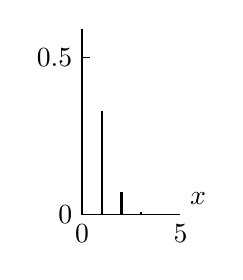
\begin{tikzpicture}[x={0.25cm},y={4cm}]
\foreach \x/\y in {0/0.59,1/0.328,2/0.0723,3/0.0081}{\draw[thick](\x,0)--++(0,\y);}
\draw(0,0)node[left]{$0$}node[below]{$0$}--(5,0)node[below]{$5$}node[above right]{$x$};
\draw(0,0.5)node[left]{$0.5$}--++(0.4,0);
\end{tikzpicture}
\caption*{$p=0.1$}
\end{subfigure}%
\begin{subfigure}{0.2\textwidth}
\centering
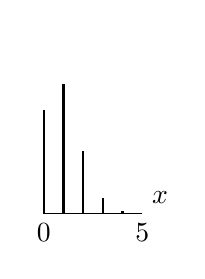
\begin{tikzpicture}[x={0.25cm},y={4cm}]
\foreach \x/\y in {0/0.328,1/0.41,2/0.2,3/0.05,4/0.0064}{\draw[thick](\x,0)--++(0,\y);}
\draw(0,0)node[below]{$0$}--(5,0)node[below]{$5$}node[above right]{$x$};
\path(0,0)--++(0,0.59);
\end{tikzpicture}
\caption*{$p=0.2$}
\end{subfigure}%
\begin{subfigure}{0.2\textwidth}
\centering
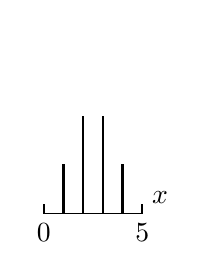
\begin{tikzpicture}[x={0.25cm},y={4cm}]
\foreach \x/\y in {0/0.031,1/0.156,2/0.31,3/0.31,4/0.156,5/0.031}{\draw[thick](\x,0)--++(0,\y);}
\draw(0,0)node[below]{$0$}--(5,0)node[below]{$5$}node[above right]{$x$};
\path(0,0)--++(0,0.59);
\end{tikzpicture}
\caption*{$p=0.5$}
\end{subfigure}%
\begin{subfigure}{0.2\textwidth}
\centering
\begin{tikzpicture}[x={0.25cm},y={4cm}]
\foreach \x/\y in {0/0,1/0.006,2/0.051,3/0.2,4/0.41,5/0.033}{\draw[thick](\x,0)--++(0,\y);}
\draw(0,0)node[below]{$0$}--(5,0)node[below]{$5$}node[above right]{$x$};
\path(0,0)--++(0,0.59);
\end{tikzpicture}
\caption*{$p=0.8$}
\end{subfigure}%
\begin{subfigure}{0.2\textwidth}
\centering
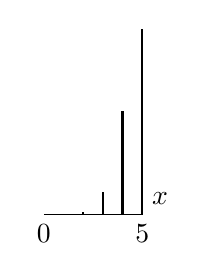
\begin{tikzpicture}[x={0.25cm},y={4cm}]
\foreach \x/\y in {0/0,1/0,2/0.008,3/0.073,4/0.33,5/0.59}{\draw[thick](\x,0)--++(0,\y);}
\draw(0,0)node[below]{$0$}--(5,0)node[below]{$5$}node[above right]{$x$};
\end{tikzpicture}
\caption*{$p=0.9$}
\end{subfigure}%
\caption{مختلف \عددی{p} اور \عددی{n=5} کے لئے مساوات \حوالہ{مساوات_شماریات_ثنائی_تقسیم_ب} میں دی گئی تثنائی تقسیم}
\label{شکل_شماریات_ثنائی_مثالیں}
\end{figure}

ثنائی تقسیم کی اوسط (سوال \حوالہ{سوال_شماریات_ثنائی_ثبوت_الف})
\begin{align}\label{مساوات_شماریات_ثنائی_تقسیم_پ}
\mu=np
\end{align}
اور تغیریت  (سوال \حوالہ{سوال_شماریات_ثنائی_ثبوت_الف})
\begin{align}\label{مساوات_شماریات_ثنائی_تقسیم_ت}
\sigma^{\,2}=npq
\end{align}
ہے۔دھیان رہے کہ \عددی{p=0.5} پر \عددی{\mu} کے لحاظ سے تقسیم تشاکلی ہے۔

\جزوحصہء{پوئسن تقسیم}
ایسی غیر مسلسل تقسیم جس کا تفاعل احتمال درج ذیل ہو \اصطلاح{پوئسن تقسیم}\فرہنگ{پوئسن!تقسیم}\فرہنگ{تقسیم!پوئسن}\حاشیہب{Poisson distribution}\فرہنگ{distribution!Poisson} کہلاتی\حاشیہد{سمیوں دنی پوسوں} ہے۔ 
\begin{align}\label{مساوات_شماریات_پوئسن_تقسیم_الف}
f(x)=\frac{\mu^x}{x!}e^{-\mu}
\end{align}
شکل \حوالہ{شکل_شماریات_پوئسن_مثالیں} میں \عددی{n=5} اور مختلف \عددی{\mu} کے لئے  مساوات \حوالہ{مساوات_شماریات_پوئسن_تقسیم_الف} میں دی گئی پوئسن تقسیم ترسیم کی گئی ہے۔\عددی{p\to 0} اور \عددی{n\to \infty} کی صورت اوسط \عددی{\mu=np} ایک متناہی قیمت کے قریب تر ہو گی اور  ثنائی تقسیم  کی  تحدیدی صورت  پوئسن تقسیم دیتی ہے۔پوئسن تقسیم کی اوسط \عددی{\mu} اور تغیریت (سوال \حوالہ{سوال_شماریات_پوئسن_ثبوت_الف}) درج ذیل ہے۔
\begin{align}\label{مساوات_شماریات_پوئسن_تقسیم_ب}
\sigma^{\,2}=\mu
\end{align}

اکائی دورانیہ (وقت) میں کسی چوک سے گزرتی گاڑیوں کی تعداد، اکائی لمبائی کے تار میں عیبوں کی تعداد، کاغذ کے اکائی رقبہ میں عیبوں کی تعداد، وغیرہ پوئسن تقسیم سے حاصل کیے جاتے ہیں۔ 
\begin{figure}
\centering
\begin{subfigure}{0.2\textwidth}
\centering
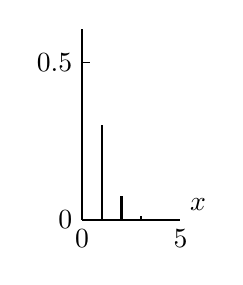
\begin{tikzpicture}[x={0.25cm},y={4cm}]
\foreach \x/\y in {0/0.607,1/0.303,2/0.076,3/0.013,4/0.0016}{\draw[thick](\x,0)--++(0,\y);}
\draw(0,0)node[left]{$0$}node[below]{$0$}--(5,0)node[below]{$5$}node[above right]{$x$};
\draw(0,0.5)node[left]{$0.5$}--++(0.4,0);
\end{tikzpicture}
\caption*{$\mu=0.5$}
\end{subfigure}%
\begin{subfigure}{0.2\textwidth}
\centering
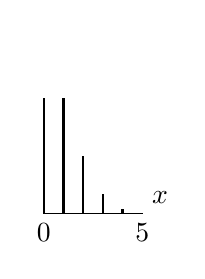
\begin{tikzpicture}[x={0.25cm},y={4cm}]
\foreach \x/\y in {0/0.368,1/0.368,2/0.184,3/0.061,4/0.015,5/0.003}{\draw[thick](\x,0)--++(0,\y);}
\draw(0,0)node[below]{$0$}--(5,0)node[below]{$5$}node[above right]{$x$};
\path(0,0)--++(0,0.59);
\end{tikzpicture}
\caption*{$\mu=1$}
\end{subfigure}%
\begin{subfigure}{0.2\textwidth}
\centering
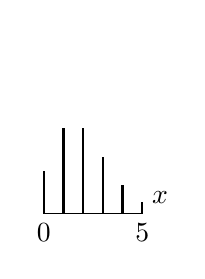
\begin{tikzpicture}[x={0.25cm},y={4cm}]
\foreach \x/\y in {0/0.135,1/0.27,2/0.27,3/0.18,4/0.09,5/0.036}{\draw[thick](\x,0)--++(0,\y);}
\draw(0,0)node[below]{$0$}--(5,0)node[below]{$5$}node[above right]{$x$};
\path(0,0)--++(0,0.59);
\end{tikzpicture}
\caption*{$\mu=2$}
\end{subfigure}%
\begin{subfigure}{0.4\textwidth}
\centering
\begin{tikzpicture}[x={0.25cm},y={4cm}]
\foreach \x/\y in {0/0.007,1/0.034,2/0.084,3/0.14,4/0.175,5/0.175,6/0.146,7/0.104,8/0.065,9/0.036,10/0.018,11/0.0082}{\draw[thick](\x,0)--++(0,\y);}
\draw(0,0)node[below]{$0$}--(11,0)node[below]{$11$}node[above right]{$x$};
\path(0,0)--++(0,0.59);
\end{tikzpicture}
\caption*{$\mu=5$}
\end{subfigure}%
\caption{مختلف \عددی{p} اور \عددی{n=5} کے لئے مساوات \حوالہ{مساوات_شماریات_پوئسن_تقسیم_الف} میں دی گئی پوئسن تقسیم}
\label{شکل_شماریات_پوئسن_مثالیں}
\end{figure}

\جزوحصہء{واپس رکھ کر اور واپس نہ رکھ کر نمونے کا حصول۔بیش ہندسی تقسیم}
واپس رکھ کر نمونہ حاصل کرنے میں ثنائی تقسیم (مثال \حوالہ{مثال_شماریات_واپس_رکھ_نہ_رکھ_کر_نمونہ}) اہم ہے۔ مثال کے طور پر ایک ڈبیا میں \عددی{N} پیچ ہیں جن میں سے \عددی{M} پیچ عیب دار ہیں۔اگر ہم ڈبے سے ایک پیچ بلا منصوبہ نکالیں تب عیب دار پیچ کے حصول کا احتمال
\begin{align*}
p=\frac{M}{N}
\end{align*}
ہو گا۔یوں واپس رکھ کر حاصل، \عددی{x} پیچوں کے نمونہ میں عیب دار پیچوں کی تعداد \عددی{x} ہونے کا احتمال (مساوات \حوالہ{مساوات_شماریات_ثنائی_تقسیم_ب})
\begin{align}\label{مساوات_شماریات_واپس_رکھ_کر_نمونہ}
f(x)=\binom{n}{x}\big(\frac{M}{N}\big)^x\big(1-\frac{M}{N}\big)^{n-x}\quad\quad (x=0,1,\cdots,n)
\end{align}
ہو گا۔واپس نہ رکھ کر حاصل نمونہ میں احتمال 
\begin{align}\label{مساوات_شماریات_بیش_ہندسی_تقسیم}
f(x)=\frac{\binom{M}{x}\binom{N-M}{n-x}}{\binom{N}{n}}\quad\quad (x=0,1,\cdots,n)
\end{align}
ہو گا۔مساوات \حوالہ{مساوات_شماریات_بیش_ہندسی_تقسیم} میں دی گئی تقسیم کو \اصطلاح{بیش ہندسی تقسیم}\فرہنگ{تقسیم!بیش ہندسی}\فرہنگ{بیش ہندسی!تقسیم}\حاشیہب{hypergeometric distribution}\فرہنگ{distribution!hypergeometric} کہتے\حاشیہد{چونکہ اس تقسیم کے معیار اثر کے پیدا کار تفاعل کو بیش ہندسی تفاعل کی صورت میں لکھا جا سکتا ہے۔} ہیں۔

مساوات \حوالہ{مساوات_شماریات_بیش_ہندسی_تقسیم} ثابت کرنے کی خاطر ہم دیکھتے ہیں کہ مساوات \حوالہ{مساوات_شماریات_مرتب_اجتماعات_ب} کے تحت 
\begin{itemize}
\item{(الف)}
\عددی{N} اشیاء میں سے \عددی{n} اشیاء کے انتخاب کے \عددی{\binom{N}{n}} مختلف طریقے ہیں،
\item{(ب)}
\عددی{M} میں سے \عددی{x} عیب دار کے انتخاب کے \عددی{\binom{M}{x}} مختلف طریقے ہیں،
\item{(پ)}
\عددی{N-M} میں سے \عددی{n-x} بے عیب کے انتخاب کے \عددی{\binom{N-M}{n-x}} مختلف طریقے ہیں،
\end{itemize}
اور (ب) میں ہر طریقہ کے ساتھ (پ) کا ہر طریقہ لے  کر، بغیر واپس رکھتے ہوئے \عددی{n} میں سے \عددی{x} عیب دار کی انتخاب کے کل طریقے حاصل ہوں گے۔چونکہ (الف) تمام وقوعات کا مجموعہ ہے اور ہم بلا منصوبہ انتخاب کرتے ہیں لہٰذا اس طرح کے ہر طریقہ کا احتمال \عددی{\tfrac{1}{\binom{N}{n}}} ہو گا۔یوں مساوات \حوالہ{مساوات_شماریات_بیش_ہندسی_تقسیم} ثابت ہوتا ہے۔

بیش ہندسی تقسیم کی اوسط (سوال \حوالہ{سوال_شماریات_اوسط_بیش_ہندسی_الف})
\begin{align}\label{مساوات_شماریات_اوسط_بیش_ہندسی_الف}
\mu=n\frac{M}{N}
\end{align}
اور تغیریت
\begin{align}
\sigma^{\,2}=\frac{nM(N-M)(N-n)}{N^2(N-1)}
\end{align}
ہے۔

%================
\ابتدا{مثال}\quad \موٹا{واپس رکھ کر اور نا رکھ کر نمونے کا حصول}\\
ایک ڈبہ میں \عددی{10} تصاویر ہیں جن میں سے \عددی{3} عیب دار ہیں۔ہم بلا منصوبہ \عددی{ 2} تصاویر ڈبے سے نکالتے ہیں۔بلا منصوبہ متغیر
\begin{align*}
X=\text{\RL{نمونہ میں عیب دار کی تعداد}}
\end{align*}
کا تفاعل احتمال تلاش کریں۔\\
حل:\quad
یہاں \عددی{N=10}، \عددی{M=3}، \عددی{N-M=7} اور \عددی{n=2} ہیں۔واپس رکھ کر نمونہ حاصل کرتے ہوئے مساوات \حوالہ{مساوات_شماریات_واپس_رکھ_کر_نمونہ} کے تحت
\begin{align*}
f(x)=\binom{2}{x}\big(\frac{3}{10}\big)^x\big(\frac{7}{10}\big)^{2-x},\quad f(0)=0.49,\quad f(1)=0.42,\quad f(2)=0.09
\end{align*}
حاصل ہوتا ہے۔ واپس نہ رکھ کر نمونہ حاصل کرتے ہوئے مساوات \حوالہ{مساوات_شماریات_بیش_ہندسی_تقسیم} سے
\begin{align*}
f(x)=\frac{\binom{3}{x}\binom{7}{2-x}}{\binom{10}{2}},\quad f(0)=f(1)=\frac{21}{45}\approx 0.47,\quad f(2)=\frac{3}{45}\approx 0.07
\end{align*}
حاصل ہوتا ہے۔
\انتہا{مثال}
%========================

اگر \عددی{n} کے لحاظ سے \عددی{N}، \عددی{M} اور \عددی{N-M} بہت بڑی مقدار ہوں تب واپس رکھتے ہوئے اور واپس نہ رکھتے ہوئے حاصل کردہ  نمونے تقریباً ایک جیسے ہوں گے لہٰذا ایسی صورت میں بیش ہندسی تقسیم کی جگہ \عددی{p=\tfrac{M}{N}} لیتے ہوئے ثنائی تقسیم استعمال کی جا سکتی ہے، جو نسبتاً سادہ تفاعل ہے۔

یوں بہت بڑی آبادی (\اصطلاح{لامتناہی آبادی}) سے،  واپس رکھتے ہوئے یا واپس نہ رکھتے ہوئے، نمونہ حاصل کرتے ہوئے ثنائی تقسیم استعمال کی جا سکتی ہے۔

%=====================
\حصہء{سوالات}
%=====================
\ابتدا{سوال}\quad
چار سکے ایک ساتھ  اچھالے جاتے ہیں۔بلا منصوبہ متغیر "\عددی{\text{\RL{تعداد خط}}=X}" کا تفاعل احتمال تلاش کریں؟ \عددی{0} خط، \عددی{1} خط، کم سے کم \عددی{1} خط اور زیادہ سے زیادہ \عددی{3}  خط کا احتمال حاصل کریں۔\\
جواب:\quad
$0.0625, 0.25, 0.9375,0.9375$
\انتہا{سوال}
%==========================
\ابتدا{سوال}\quad
نشانے پر تیر مارنے کا امکان \عددی{\SI{10}{\percent}} ہے۔ \عددی{10} تیر چلائے جاتے ہیں۔کم سے کم ایک بار نشانہ لگنے کا احتمال کیا ہو گا؟
\انتہا{سوال}
%========================
\ابتدا{سوال}\quad
\عددی{24} گھنٹوں کے پرکھ میں \عددی{p=\SI{1}{\percent}} امکان ہے کہ ایک خاص قسم کا بلب زائل ہو جائے گا۔ایسے \عددی{10} بلبوں کا ،کوئی بھی بلب خراب ہوئے بغیر، مسلسل \عددی{24} گھنٹے  روشنی دینے کا احتمال کیا ہو گا۔\\
جواب:\quad
$0.99^{10}\approx \SI{90.4}{\percent}$
\انتہا{سوال}
%=========================
\ابتدا{سوال}\شناخت{سوال_شماریات_ثنائی_ثبوت_الف}\quad
مسئلہ ثنائی استعمال کرتے ہوئے دکھائیں کہ ثنائی تقسیم کے  معیار اثر کا پیدا کار تفاعل (سوال \حوالہ{سوال_شماریات_معیار_اثر_پیدا_کار_تفاعل_الف}) درج ذیل ہے اور مساوات \حوالہ{مساوات_شماریات_ثنائی_تقسیم_پ} اور مساوات \حوالہ{مساوات_شماریات_ثنائی_تقسیم_ت} کو ثابت کریں۔
\begin{align*}
G(t)=\sum_{x=0}^{n}e^{tx}\binom{n}{x}p^xq^{n-x}=\sum_{x=0}^{n}\binom{n}{x}(pe^t)^xq^{n-x}=(pe^t+q)^n
\end{align*}  
\انتہا{سوال}
%===========================
\ابتدا{سوال}\شناخت{سوال_شماریات_پوئسن_ثبوت_الف}\quad
دکھائیں کہ پوئسن تقسیم کے  معیار اثر کا پیدا کار تفاعل  درج ذیل ہے اور مساوات \حوالہ{مساوات_شماریات_پوئسن_تقسیم_ب} کو ثابت کریں۔
\begin{align*}
G(t)=e^{-\mu}e^{\mu e^t}
\end{align*}  
\انتہا{سوال}
%===========================
\ابتدا{سوال}\quad
دکھائیں کہ \عددی{E([X-\mu]^3)=E(X^3)-3\mu E(X^2)+2\mu^3} ہو گا۔اس کو اور سوال \حوالہ{سوال_شماریات_پوئسن_ثبوت_الف} کو استعمال کرتے ہوئے  دکھائیں کہ پوئسن تقسیم کا ترچھاپن \عددی{\gamma=\tfrac{1}{\sqrt{\mu}}} ہے جو کہتا ہے کہ \عددی{\mu} کی بڑی قیمت کے لئے یہ تقسیم تقریباً تشاکلی ہے (شکل \حوالہ{شکل_شماریات_پوئسن_مثالیں})۔
\انتہا{سوال}
%============================
\ابتدا{سوال}\quad
دکھائیں کہ پوئسن تقسیم کا تفاعل تقسیم \عددی{F(\infty)=1} کو مطمئن کرتا ہے۔
\انتہا{سوال}
%==========================
\ابتدا{سوال}\quad
ایک ٹیلیفون تقسیم کار تختی اوسطاً \عددی{600} ٹیلیفون کے لئے کافی ہے۔ یہ ایک منٹ میں زیادہ سے زیادہ \عددی{10} نئے ٹیلیفون ملا سکتی ہے۔پوئسن تقسیم استعمال کرتے ہوئے اس بات کا احتمال تلاش کریں کہ کسی ایک منٹ میں یہ تقسیم کار تختی نا کافی ثابت ہو گا۔
\انتہا{سوال}
%=======================
\ابتدا{سوال}\quad
ایک کارخانے میں \عددی{\SI{50}{\ohm}} کے برقی مزاحمت پیدا کیے جاتے ہیں جن میں سے وہ مزاحمت بے عیب تصور کیے جاتے ہیں جن کی مزاحمت \عددی{\SI{45}{\ohm}} اور \عددی{\SI{55}{\ohm}} کے بیچ ہو۔عیب دار مزاحمت کا احتمال \عددی{\SI{0.2}{\percent}} ہے۔ان مزاحمتوں کو \عددی{100} کی کھیپ میں، ضمانت کے ساتھ فروخت کیا جاتا ہے۔تقسیم پوئسن استعمال کرتے ہوئے ایک کھیپ میں عیب دار مزاحمت نکلنے کا احتمال حاصل کریں۔\\
جواب:\quad
$1-e^{-0.2}=0.1813$
\انتہا{سوال}
%==========================
\ابتدا{سوال}\quad
فرض کریں کہ ایک مشین کے پیدا کردہ پیچوں میں سے  \عددی{\SI{3}{\percent}} عیب دار ہوتے ہیں۔ایک ڈبیا میں \عددی{50} پیچ بھرے جاتے ہیں۔تقسیم پوئسن استعمال کرتے ہوئے ایک ڈبیا میں \عددی{x} عیب دار پیچ نکلنے کا احتمال تلاش کریں۔
\انتہا{سوال}
%=============================
\ابتدا{سوال}\quad
ایک پل سے جمع کے دن صبح \عددی{8} تا \عددی{10} بجے  فی منٹ \عددی{X} گاڑیاں گزرتی ہیں۔فرض کریں کہ \عددی{X} کو پوئسن تقسیم ظاہر کرتی ہے جس کا اوسط \عددی{5} ہے۔کسی ایک منٹ میں \عددی{3} یا \عددی{3} سے کم گاڑیاں گزرنے کا احتمال تلاش کریں۔\\
جواب:\quad
$0.265$
\انتہا{سوال}
%================================
\ابتدا{سوال}\quad
ایک مقناطیسی پٹی کے \عددی{100} میٹر لمبائی میں اوسطاً \عددی{2} عیب پائے جاتے ہیں۔ \عددی{300} میٹر لمبی پٹی (الف) میں \عددی{x} عیب کا احتمال کیا ہو گا، (ب) بلا عیب ہونے کا احتمال کیا ہو گا؟ 
\انتہا{سوال}
%=============================
\ابتدا{سوال}\quad
گتے کے ڈبا میں \عددی{20} فتیلہ ہیں جن میں سے \عددی{5} عیب دار ہیں۔ اس ڈبا سے بلا منصوبہ \عددی{3} فتیلے بغیر واپس رکھے  بطور نمونہ نکالے جاتے ہیں۔اس نمونہ میں \عددی{x} عیب دار فتیلے ہونے کا احتمال کیا ہو گا؟
\انتہا{سوال}
%=======================
\ابتدا{سوال}\شناخت{سوال_شماریات_قلم_الف}\quad
ایک  تقسیم کار \عددی{100} قلم کے ڈبوں فروخت کرتا ہے۔وہ اس بات کی ضمانت دیتا ہے کہ کسی ایک ڈبے میں سے زیادہ سے زیادہ \عددی{\SI{10}{\percent}} قلم عیب دار ہوں گے۔ایک خریدار ہر ڈبے میں سے \عددی{10} قلم بغیر واپس رکھے نکال کر پرکھتا ہے۔کوئی بھی قلم عیب دار نہ ہونے کی صورت میں وہ ڈبا خرید لیتا ہے ورنہ وہ ڈبے کو نہیں خریدتا۔اس کا کیا احتمال ہے کہ ایک ڈبے میں \عددی{10} عیب دار قلم ہوں (لہٰذا یہ ضمانت پر پورا اترتا ہے) اور خریدار اس ڈبے کو نہ خریدے؟
\انتہا{سوال}
%=========================
\ابتدا{سوال}\quad
سوال \حوالہ{سوال_شماریات_قلم_الف} میں کیا احتمال ہے کہ ایک ڈبے میں \عددی{20} عیب دار قلم ہونے کے باوجود خریدار اسے خرید لیتا ہے؟
\انتہا{سوال}
%============================
\ابتدا{سوال}\quad
ایک کارخانے میں پیچوں کی پیداوار کی جاتی ہے۔ہر گھنٹہ بلا منصوبہ \عددی{n} پیچ کا نمونہ حاصل کر کے پرکھا جاتا ہے۔ایک یا ایک سے زیادہ عیب دار پیچ حاصل ہونے کی صورت میں کام روک کر مشینوں کی کارکردگی تسلی بخش بنائی جاتی ہے۔\عددی{n} کتنا ہو گا اگر  \عددی{\SI{10}{\percent}} عیب دار پیچ کی صورت میں \عددی{\SI{95}{\percent}} احتمال ہے کہ کام روکا جائے گا؟  
\انتہا{سوال}
%======================
\ابتدا{سوال}\quad
\عددی{1} سے لے کر \عددی{13} تک عدد کو علیحدہ علیحدہ کاغذ پر لکھا جاتا ہے۔ان میں سے بلا منصوبہ تین کاغذ نکالے جاتے ہیں جبکہ  ایک شخص  بغیر دیکھے  تینوں پر لکھے اعداد بتاتا ہے۔کیا احتمال ہے کہ وہ (الف) کوئی بھی درست عدد نہ بتائے، (ب) ایک عدد ٹھیک بتائے، (پ) دو عدد ٹھیک بتائے، (ت) تینوں اعداد ٹھیک بتائے؟  \\
جواب:\quad
$\tfrac{120}{286},\tfrac{135}{286},\tfrac{30}{286},\tfrac{1}{286}$ 
\انتہا{سوال}
%====================
\ابتدا{سوال}\شناخت{سوال_شماریات_اوسط_بیش_ہندسی_الف}\quad
مساوات \حوالہ{مساوات_شماریات_اوسط_بیش_ہندسی_الف} کو ثابت کریں۔
\انتہا{سوال}
%===========================
\ابتدا{سوال}\quad \موٹا{(متعدد رکنی تقسیم)}\quad
\عددی{k}  باہمی بلا شرکت وقوعات \عددی{A_1,\cdots,A_k} کے احتمال بالترتیب \عددی{p_1,\cdots,p_k} ہیں  جہاں \عددی{p_1+\cdots+p_k=1} ہے۔فرض کریں کہ \عددی{n} باہمی بلا شرکت کوشش کیے جاتے ہیں۔دکھائیں کہ ان میں \عددی{A_1} کی تعداد \عددی{x_1}، \نقطے، \عددی{A_k} کی تعداد \عددی{x_k} ہونے کا احتمال
\begin{align*}
f(x_1,\cdots,x_n)=\frac{n!}{x_1!\cdots x_k!}p_1^{x_1}\cdots p_k^{x_k}
\end{align*}
ہو گا جہاں \عددی{0\le x_j\le n}، \عددی{j=1,\cdots,k}، اور \عددی{x_1+\cdots+x_n=n} ہیں۔ایسی تقسیم جس کی تفاعل تقسیم درج بالا ہو کو \ترچھا{متعدد رکنی تقسیم}\فرہنگ{تقسیم!متعدد رکنی}\حاشیہب{multinomial distribution}\فرہنگ{distribution!multinomial} کہتے ہیں۔
\انتہا{سوال}
%=============================
\ابتدا{سوال}\quad
برقی مزاحمت کی پیداوار میں \عددی{\SI{3}{\percent}} کی مزاحمت \عددی{R<\SI{198}{\ohm}} اور \عددی{\SI{5}{\percent}} کی مزاحمت \عددی{R>\SI{201}{\ohm}} ہے۔بلا منصوبہ \عددی{20} مزاحمتوں کے نمونہ میں \عددی{R<\SI{198}{\ohm}} کے \عددی{x_1} اور \عددی{R>\SI{201}{\ohm}} کے \عددی{x_2} مزاحمت حاصل کرنے کا احتمال کیا ہو گا؟
\انتہا{سوال}
%===============================

\حصہ{عمومی تقسیم}\شناخت{حصہ_شماریات_عمومی_تقسیم}
ایسی تقسیم جس کی کثافت
\begin{align}\label{مساوات_شماریات_عمومی_تقسیم_الف}
f(x)=\frac{1}{\sigma\sqrt{2\pi}}\,e^{-\frac{1}{2}(\frac{x-\mu}{\sigma})^2}\quad\quad\quad (\sigma>0)
\end{align}
ہو کو \اصطلاح{عمومی تقسیم}\فرہنگ{تقسیم!عمومی}\حاشیہب{normal distribution}\فرہنگ{distribution!normal} یا \ترچھا{گاوسی تقسیم}\فرہنگ{تقسیم!گاوسی}\فرہنگ{گاوس!گاوسی تقسیم}\حاشیہب{Gauss distribution}\فرہنگ{distribution!Gauss} کہتے ہیں۔اس طرح تقسیم والا بلا منصوبہ متغیر \اصطلاح{عمومی}\فرہنگ{عمومی}\حاشیہب{normal}\فرہنگ{normal} یا \اصطلاح{عمومی بانٹا ہوا}\فرہنگ{عمومی!بانٹا ہوا}\حاشیہب{normally distributed}\فرہنگ{normally distributed} کہلاتا ہے۔عملی دلچسپی کے بہت سارے بلا منصوبہ متغیرات عمومی یا تخمیناً عمومی ہیں اور یا ان کا تبادلہ با آسانی عمومی بلا منصوبہ متغیرات میں کیا جا سکتا ہے۔ اس کے علاوہ کئی پیچیدہ تقسیم کو تخمیناً عمومی تقسیم سے ظاہر کیا جا سکتا ہے۔شماریاتی پرکھ کے کئی ثبوت میں بھی یہ تقسیم کردار ادا کرتی ہے۔   


مساوات \حوالہ{مساوات_شماریات_عمومی_تقسیم_الف} میں تقسیم کی اوسط \عددی{\mu}  اور اس کا معیاری انحراف \عددی{\sigma}  ہے۔ \عددی{f(x)} کی منحنی \عددی{\mu} کے لحاظ سے تشاکلی ہے اور اس  کو \اصطلاح{قوس جرس}\فرہنگ{قوس!جرس}\فرہنگ{جرس!قوس}\حاشیہب{bell curve}\فرہنگ{bell curve} کہتے ہیں۔قوس جرس کو شکل \حوالہ{شکل_شماریات_عمومی_تقسیم} میں \عددی{\mu=0} اور \عددی{\sigma} کے کئی قیمتوں کے لئے دکھایا گیا ہے۔ \عددی{\mu>0} (\عددی{\mu<0}) کے لئے قوس کی شکل تبدیل نہیں ہوتی البتہ یہ \عددی{\abs{\mu}} اکائیاں دائیں (بائیں) منتقل ہوتا ہے۔\عددی{\sigma^{\,2}} کی قیمت جتنی کم ہو،\عددی{x=\mu} پر قوس کی چوٹی اتنی زیادہ بلند ہو گی اور چوٹی کے دونوں اطراف ڈھلوان اتنی زیادہ ہو گی (شکل \حوالہ{شکل_شماریات_عمومی_تقسیم}) جو تغیریت کے تصور کے عین مطابق ہے۔
\begin{figure}
\centering
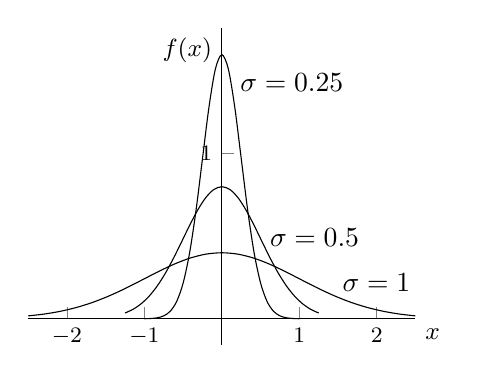
\begin{tikzpicture}
\begin{axis}[small,axis lines*=middle,ytick={1},yticklabels={$1$},xmin=-2.5,xmax=2.5,xlabel={$x$},x label style={at={(current axis.right of origin)},anchor=north west},ylabel={$f(x)$},y label style={rotate=-90},y label style={at={(current axis.above origin)},anchor=north east}]
\addplot[smooth,domain=-1:1] {1/(0.25*sqrt(2*pi))*e^(-0.5*((x-0)/0.25)^2)}node[pos=0.55,right]{$\sigma=0.25$};
\addplot[smooth,domain=-1.25:1.25] {1/(0.5*sqrt(2*pi))*e^(-0.5*((x-0)/0.5)^2)}node[pos=0.7,right]{$\sigma=0.5$};
\addplot[smooth,domain=-2.5:2.5] {1/(1*sqrt(2*pi))*e^(-0.5*((x-0)/1)^2)}node[pos=0.9,above,yshift={0.1cm}]{$\sigma=1$};
\end{axis}
\end{tikzpicture}
\caption{عمومی تقسیم  کی کثافت (مساوات \حوالہ{مساوات_شماریات_عمومی_تقسیم_الف}) برائے \عددی{\mu=0} اور مختلف \عددی{\sigma}}
\label{شکل_شماریات_عمومی_تقسیم}
\end{figure}

مساوات \حوالہ{مساوات_شماریات_عمومی_تقسیم_الف} سے ہم دیکھتے ہیں کہ عمومی تقسیم کا تقسیمی تفاعل
\begin{align}\label{مساوات_شماریات_عمومی_تقسیم_ب}
F(x)=\frac{1}{\sigma\sqrt{2\pi}}\int_{-\infty}^{x}e^{-\frac{1}{2}(\frac{v-\mu}{\sigma})^2}\dif v
\end{align}
ہو گا۔یوں مساوات \حوالہ{مساوات_شماریات_استمراری_بلا_منصوبہ_متغیر_پ} سے درج ذیل حاصل ہو گا۔
\begin{align}\label{مساوات_شماریات_عمومی_تقسیم_پ}
P(a<X\le b)=F(b)-F(a)=\frac{1}{\sigma\sqrt{2\pi}}\int_{a}^{b}e^{-\frac{1}{2}(\frac{v-\mu}{\sigma})^2}\dif v
\end{align}

\begin{figure}
\centering
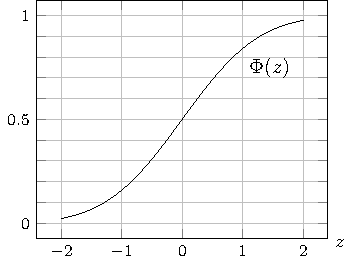
\includegraphics{normalDistributionFunctionWithZeroMeanOneVariance}
\caption{اوسط $0$ اور تغیریت $1$ کے عمومی تقسیم کا  تفاعل تقسیم $\Phi(z)$}
\label{شکل_شماریات_عمومی_تقسیم_صفر_اوسط_اکائی_تغیریت}
\end{figure}
مساوات \حوالہ{مساوات_شماریات_عمومی_تقسیم_ب} کا تکمل بنیادی طریقوں سے حاصل کرنا ممکن نہیں ہے البتہ اس کو درج ذیل تکمل کی صورت میں لکھا جا سکتا ہے (شکل \حوالہ{شکل_شماریات_عمومی_تقسیم_صفر_اوسط_اکائی_تغیریت})
\begin{align}\label{مساوات_شماریات_عمومی_تقسیم_ت}
\Phi(z)=\frac{1}{\sqrt{2\pi}}\int_{-\infty}^{z}e^{-\frac{u^2}{2}}\dif u
\end{align}
جو عمومی تقسیم کا وہ تفاعل ہے جس کی اوسط \عددی{0} اور تغیریت \عددی{1} ہے اور جس کو جدول بند کیا گیا ہے۔ یہ جدول ضمیمہ \حوالہ{ضمیمہ_جدول} میں پیش کیے گئے ہیں۔اگر \عددی{\tfrac{v-\mu}{\sigma}=u} لیا جائے تب \عددی{\tfrac{\dif u}{\dif v}=\tfrac{1}{\sigma}} اور \عددی{\dif v=\sigma \dif u} ہو گا اور ہمیں \عددی{-\infty} تا \عددی{z=\tfrac{x-\mu}{\sigma}} تکمل لینا ہو گا۔مساوات \حوالہ{مساوات_شماریات_عمومی_تقسیم_ب} سے یوں
\begin{align*}
F(x)=\frac{1}{\sigma\sqrt{2\pi}}\int_{-\infty}^{\frac{x-\mu}{\sigma}}e^{-\frac{u^2}{2}}\sigma \dif u
\end{align*}
حاصل ہو گا جس میں \عددی{\sigma} کٹ جاتا ہے اور جس کا دایاں ہاتھ مساوات \حوالہ{مساوات_شماریات_عمومی_تقسیم_ت} دیتا ہے جہاں  \عددی{z=\tfrac{x-\mu}{\sigma}} ہے یعنی:
\begin{align}\label{مساوات_شماریات_عمومی_تقسیم_ٹ}
F(x)=\Phi\big(\frac{x-\mu}{\sigma}\big)
\end{align}
اس سے اور مساوات \حوالہ{مساوات_شماریات_عمومی_تقسیم_پ} سے درج ذیل ایک اہم کلیہ  اخذ ہوتا ہے۔
\begin{align}\label{مساوات_شماریات_عمومی_تقسیم_ث}
P(a<X\le b)=F(b)-F(a)=\Phi\big(\frac{b-\mu}{\sigma}\big)-\Phi\big(\frac{a-\mu}{\sigma}\big)
\end{align}
بالخصوص \عددی{a=\mu-\sigma} اور \عددی{b=\mu+\sigma} کی صورت میں دایاں ہاتھ \عددی{\Phi(1)-\Phi(-1)} کے برابر ہے؛  
\عددی{a=\mu-2\sigma} اور \عددی{b=\mu+2\sigma} کی صورت میں دایاں ہاتھ \عددی{\Phi(2)-\Phi(-2)} کے برابر ہے، وغیرہ، وغیرہ۔تفاعل \عددی{\Phi(z)} کی قیمتیں جدول سے دیکھتے ہوئے درج ذیل حاصل ہوتا ہے (شکل \حوالہ{شکل_شماریات_اظہار_عمومی_تقسیم})۔
\begin{gather}
\begin{aligned}\label{مساوات_شماریات_عمومی_تقسیم_ج}
\text{(الف)}\quad P(\mu-\sigma<X\le \mu+\sigma)&\approx \SI{68}{\percent}\\
\text{(ب)}\quad P(\mu-2\sigma<X\le \mu+2\sigma)&\approx \SI{95.5}{\percent}\\
\text{(پ)}\quad P(\mu-3\sigma<X\le \mu+3\sigma)&\approx \SI{99.7}{\percent}
\end{aligned}
\end{gather}
%
\begin{figure}
\centering
\begin{subfigure}{0.5\textwidth}
\centering
\begin{tikzpicture}
\begin{axis}[small,axis lines*=middle,axis y line=none,yticklabels={$1$},xlabel={$x$},x label style={at={(current axis.right of origin)},anchor=north west},ylabel={$f(x)$},y label style={rotate=-90},y label style={at={(current axis.above origin)},anchor=north east},xtick={-0.25,0,0.25},xticklabels={$\mu-\sigma$,$\mu$,$\mu+\sigma$},axis on top]
\addplot[domain=-0.25:0.25,mark=none,fill,color=lgray]{1/(0.25*sqrt(2*pi))*e^(-0.5*((x-0)/0.25)^2)}\closedcycle;
\addplot[smooth,domain=-0.6:0.6] {1/(0.25*sqrt(2*pi))*e^(-0.5*((x-0)/0.25)^2)};
\draw(axis cs:0,0.75)node[fill=white,font=\footnotesize]{$\SI{68}{\percent}$};
\draw(axis cs:-0.375,0.2)node[font=\footnotesize]{$\SI{16}{\percent}$};
\draw(axis cs:0.375,0.2)node[font=\footnotesize]{$\SI{16}{\percent}$};
\end{axis}
\end{tikzpicture}
\end{subfigure}%
\begin{subfigure}{0.5\textwidth}
\centering
\begin{tikzpicture}
\begin{axis}[small,axis lines*=middle,axis y line=none,yticklabels={$1$},xlabel={$x$},x label style={at={(current axis.right of origin)},anchor=north west},ylabel={$f(x)$},y label style={rotate=-90},y label style={at={(current axis.above origin)},anchor=north east},xtick={-0.5,0,0.5},xticklabels={$\mu-2\sigma$,$\mu$,$\mu+2\sigma$},axis on top]
\addplot[domain=-0.5:0.5,mark=none,fill,color=lgray]{1/(0.25*sqrt(2*pi))*e^(-0.5*((x-0)/0.25)^2)}\closedcycle;
\addplot[smooth,domain=-0.6:0.6] {1/(0.25*sqrt(2*pi))*e^(-0.5*((x-0)/0.25)^2)};
\draw(axis cs:0,0.75)node[fill=white,font=\footnotesize]{$\SI{95.5}{\percent}$};
\draw[stealth-](axis cs:-0.55,0.05) to [out=135,in=-90] (axis cs:-0.575,0.3)node[above,font=\footnotesize]{$\SI{2.25}{\percent}$};
\draw[stealth-](axis cs:0.55,0.05) to [out=45,in=-90] (axis cs:0.575,0.3)node[above,font=\footnotesize]{$\SI{2.25}{\percent}$};
\end{axis}
\end{tikzpicture}
\end{subfigure}%
\caption{اظہار مساوات \حوالہ{مساوات_شماریات_عمومی_تقسیم_ج}}
\label{شکل_شماریات_اظہار_عمومی_تقسیم}
\end{figure}
یوں ہم توقع کرتے ہیں کہ بلا منصوبہ عمومی متغیر \عددی{X} کی بہت ساری قیمتیں درج ذیل طرح بانٹی گئی ہوں گی۔
\begin{itemize}
\item{(الف)}
تقریباً \عددی{\tfrac{2}{3}} قیمتیں \عددی{\mu-\sigma} اور \عددی{\mu+\sigma} کے بیچ ہوں گی،
\item{(ب)}
تقریباً \عددی{\SI{95}{\percent}} قیمتیں \عددی{\mu-2\sigma} اور \عددی{\mu+2\sigma} کے بیچ ہوں گی،
\item{(پ)}
تقریباً \عددی{99\tfrac{3}{4}\si{\percent}} قیمتیں \عددی{\mu-3\sigma} اور \عددی{\mu+3\sigma} کے بیچ ہوں گی
\end{itemize}
جس کو درج ذیل طریقہ سے بھی بیان کیا جا سکتا ہے۔

وہ قیمت جس کی \عددی{\mu} سے دوری \عددی{\sigma}  سے زیادہ ہو، \عددی{3} کوششوں میں تقریباً   \عددی{1} مرتبہ واقع ہو گی، جبکہ  وہ قیمت جس کی \عددی{\mu} سے دوری \عددی{2\sigma} یا \عددی{3\sigma}  سے زیادہ ہو، بالترتیب \عددی{20}  اور \عددی{400} کوششوں  میں تقریباً   \عددی{1} مرتبہ واقع ہو گی۔یوں عملی طور پر تمام قیمتیں \عددی{\mu-3\sigma} اور \عددی{\mu+3\sigma} کے بیچ پائی جائیں گی۔اس دو اعداد کو \اصطلاح{تین سگما حدود}\فرہنگ{تین سگما حدود}\حاشیہب{three-sigma limits}\فرہنگ{limit!three-sigma} کہتے ہیں۔

اسی طرح درج ذیل حاصل ہو گا۔
\begin{gather}
\begin{aligned}\label{مساوات_شماریات_چند_نتائج}
\text{(الف)}\quad P(\mu-1.96\sigma<X\le \mu+1.96\sigma)&=\SI{95}{\percent}\\
\text{(ب)}\quad P(\mu-2.58\sigma<X\le \mu+2.58\sigma)&=\SI{99}{\percent}\\
\text{(پ)}\quad P(\mu-3.29\sigma<X\le \mu+3.29\sigma)&=\SI{99.9}{\percent}
\end{aligned}
\end{gather}

درج ذیل مثال ضمیمہ \حوالہ{ضمیمہ_جدول} میں دیے گیے عمومی تقسیم کی جدول کا استعمال سمجھنے میں مدد دیں گی۔

%================
\ابتدا{مثال}
درج ذیل احتمال ضمیمہ \حوالہ{ضمیمہ_جدول} کی مدد سے تلاش کریں جہاں \عددی{X} عمومی ہے جس کی اوسط \عددی{0} اور تغیریت \عددی{1} ہے۔
\begin{align*}
\text{(الف)}\,\,P(X\le 2.44),\,\, \text{(ب)}\,\,P(X\le -1.16),\,\,\text{(پ)}\,\,P(X\ge 1),\,\, \text{(ت)}\,\,P(2\le X\le 10)
\end{align*}
حل:\quad ہم ضمیمہ \حوالہ{ضمیمہ_جدول} سے جوابات پڑھ کر لکھتے ہیں۔
\begin{align*}
\text{(الف)}\,\,0.9927,\quad \text{(ب)}\,\,0.1230, \quad \text{(پ)}\,\,1-P(X\le 1)=1-0.8413=0.1587,\\
\text{(ت)}\,\,\Phi(10)=1.0000 \,\text{(کیوں؟)}, \Phi(2)=0.9772,\Phi(10)-\Phi(2)=0.0228
\end{align*}
\انتہا{مثال}
%======================
\ابتدا{مثال}\quad
گزشتہ مثال کو دوبارہ حل کریں۔اس مرتبہ فرض کریں کہ \عددی{X}عمومی ہے جس کی اوسط \عددی{0.8} اور تغیریت \عددی{4} ہے۔\\
جواب:\quad
ضمیمہ \حوالہ{ضمیمہ_جدول} اور مساوات \حوالہ{مساوات_شماریات_عمومی_تقسیم_ث} استعمال کرتے ہوئے درج ذیل حاصل ہو گا۔
\begin{align*}
& \text{(الف)} \quad F(2.44)=\Phi(\frac{2.44-0.80}{2})=\Phi(0.82)=0.7939\\
& \text{(ب)} \quad F(-1.16)=\Phi(-0.98)=0.1635\\
& \text{(پ)} \quad 1-P(X\le 1)=1-F(1)=1-\Phi(0.1)=0.4602\\
& \text{(ت)} \quad F(10)-F(2)=\Phi(4.6)-\Phi(0.6)=1-0.7257=0.2743
\end{align*}
\انتہا{مثال}
%========================
\ابتدا{مثال}\quad
فرض کریں کہ \عددی{X} عمومی ہے جس کی اوسط \عددی{0} اور تغیریت \عددی{1} ہے۔ایسا مستقل \عددی{c} تلاش کریں جو درج ذیل کو مطمئن کرتا ہو۔
\begin{align*}
\text{(الف)}  \,\, P(X\ge c)&=\SI{10}{\percent},\quad \text{(ب)}  \,\,P(X\le c)=\SI{5}{\percent}\\
\text{(پ)}  \,\, P(0\le X\le c)&=\SI{45}{\percent},\quad \text{(ت)} \,\,P(-c\le X\le c)=\SI{99}{\percent}
\end{align*}
حل:\quad
ضمیمہ \حوالہ{ضمیمہ_جدول} سے  درج ذیل حاصل ہو گا۔
\begin{align*}
\text{(الف)}  \quad & 1-P(X\le c)=1-\Phi(c)=0.1, \Phi(c)=0.9, c=1.282,\\
\text{(ب)}  \quad & c=-1.645,\\
\text{(پ)} \quad &\Phi(c)-\Phi(0)=\Phi(c)-0.5=0.45,\Phi(c)=0.95,c=1.645,\\
\text{(ت)} \quad & c=2.576
\end{align*}
\انتہا{مثال}
%=========================
\ابتدا{سوال}\quad
فرض کریں کہ \عددی{X} عمومی ہے جس کی اوسط \عددی{-2} اور تغیریت \عددی{0.25} ہے۔ایسا \عددی{c} تلاش کریں جو درج ذیل کو مطمئن کرتا ہو۔
\begin{align*}
\text{(الف)} \,\,&P(X\ge c)=0.2,\quad \text{(ب)} \,\,P(-c\le X\le -1)=0.5\\
\text{(پ)} \,\,&P(-2-c\le X\le -2+c)=0.9,\quad \text{(ت)} \,\,P(-2-c\le X\le -2+c)=\SI{99.6}{\percent}
\end{align*}
حل:\quad
ضمیمہ \حوالہ{ضمیمہ_جدول} سے  درج ذیل حاصل ہو گا۔
\begin{align*}
&\text{(الف)}  \,\, 1-P(X\le c)=1-\Phi(\frac{c+2}{0.5})=0.2,\\
&\quad \quad \Phi(2c+4)=0.8, 2c+4=0.842,c=-1.579\\
&\text{(ب)}  \,\, \Phi(\frac{-1+2}{0.5})-\Phi(\frac{-c+2}{0.5})=0.9772-\Phi(4-2c)=0.5,\\
&\quad \quad \Phi(4-2c)=0.4772, 4-2c=-0.057, c=2.03\\
&\text{(پ)}  \,\,\Phi(\frac{-2+c+2}{0.5})-\Phi(\frac{-2-c+2}{0.5})\\
&\quad \quad =\Phi(2c)-\Phi(-2c)=0.9,2c=1.645,c=0.823\\
&\text{(ت)}  \,\,\Phi(2c)-\Phi(-2c)=\SI{99.6}{\percent}, 2c=2.878,c=1.439
\end{align*}
\انتہا{سوال}
%=========================
\ابتدا{مثال}\شناخت{مثال_شماریات_لوہے_کی_چادر}\quad
ایک کارخانے میں ایک خاص موٹائی کی لوہے کی چادریں بنائی جاتی ہیں۔یہ کام خود کار مشین کرتے ہیں۔ خام مال میں فرق اور درجہ حرارت، لرزش وغیرہ کی بنا  مشینوں کا رویہ اور استعمال آلات میں معمولی تبدیلیاں رو نما ہوتی ہیں جنہیں قبل از وقت جاننا ممکن نہیں ہوتا ہے۔ان وجوہات کی بنا چادریں ایک دوسرے سے مختلف ہوتی ہیں۔یوں ہم چادر کی موٹائی \عددی{X} (ملی میٹر) کو بلا منصوبہ متغیر تصور کر سکتے ہیں۔ہم فرض کرتے ہیں کہ یہ متغیر عمومی ہے جس کی اوسط \عددی{\mu=\SI{10}{\milli\meter}} اور معیاری انحراف \عددی{\sigma=\SI{0.02}{\milli\meter}} ہے۔ہم عیب دار چادروں کی تعداد جاننا چاہیں گے۔عیب دار چادر وہ چادر ہے  جس کی موٹائی (الف) \عددی{\SI{9.97}{\milli\meter}} سے کم ہو، (ب) \عددی{\SI{10.05}{\milli\meter}} سے زیادہ ہو، (پ) کا اوسط (\عددی{\SI{10}{\milli\meter}}) سے انحراف \عددی{\SI{0.03}{\milli\meter}} سے زیادہ ہو۔ (ت) ہم اعداد \عددی{10-c} اور \عددی{10+c} منتخب کرنا چاہتے ہیں کہ عیب دار چادروں کی تعداد \عددی{\SI{5}{\percent}} سے زیادہ نہ ہو۔(ٹ) جزو-ت میں
 \عددی{\mu=\SI{10.01}{\milli\meter}} کرنے سے عیب دار کی فی صد تعداد پر کیا اثر پڑے گا؟

حل:\quad
 ضمیمہ \حوالہ{ضمیمہ_جدول} استعمال کرتے ہوئے درج ذیل نتائج حاصل ہوتے ہیں۔
\begin{align*}
\text{(الف)}\quad P(X\le 9.97)=\Phi(\frac{9.97-10.00}{0.02})=\Phi(-1.5)=0.0668\approx \SI{6.7}{\percent}\\
\text{(ب)} \quad P(X\ge 10.05)=1-P(X\le 10.05)=1-\Phi(\frac{10.05-10.00}{0.02})\\
=1-\Phi(2.5)=1-0.9938\approx \SI{0.6}{\percent}\\
\text{(پ)}  \quad P(9.97\le X\le 10.03)=\Phi(\frac{10.03-10.00}{0.02})-\Phi(\frac{9.97-10.00}{0.02})\\
=\Phi(1.5)-\Phi(-1.5)=0.8664; \implies 1-0.8664\approx \SI{13}{\percent}
\end{align*}
(ت) مساوات \حوالہ{مساوات_شماریات_چند_نتائج}-الف سے
\begin{align*}
c=1.96\sigma=0.039
\end{align*}
یوں جواب \عددی{\SI{9.961}{\milli\meter}} اور \عددی{\SI{10.039}{\milli\meter}} ہے۔\\
\begin{align*}
\text{(ٹ)} \quad P(9.961\le X\le 10.039)=\Phi(\frac{10.039-10.010}{0.02})-\Phi(\frac{9.961-10.010}{0.02})\\
=\Phi(1.45)-\Phi(-2.45)=0.9265-0.0071\approx \SI{92}{\percent}
\end{align*}
لہٰذا جواب \عددی{\SI{8}{\percent}} ہو گا۔آپ نے دیکھا کہ مشین میں معمولی تبدیلی سے عیب دار چادروں کی تعداد میں بہت زیادہ اضافہ پیدا ہوتا ہے۔

\انتہا{مثال}
%============================

بلا منصوبہ عمومی متغیر سے خطی تبادل کے ذریعہ بلا منصوبہ عمومی متغیر  ہی حاصل ہو گا۔مساوات \حوالہ{مساوات_شماریات_عمومی_تقسیم_ٹ} سے آپ یقیناً درج ذیل حاصل کر پائیں گے۔

%================
\ابتدا{مسئلہ}\شناخت{مسئلہ_شماریات_خطی_تبادل_دوسرا}\quad \موٹا{(خطی تبادل)}\\
اگر \عددی{X} عمومی ہو اور اس کی اوسط \عددی{\mu} اور تغیریت \عددی{\sigma^{\,2}} ہو تب \عددی{X^*=c_1X+c_2\,\, (c_1\ne 0)} عمومی ہو گا جس کی اوسط \عددی{\mu^*=c_1\mu+c_2} اور تغیریت \عددی{\sigma^{*2}=c_1^2\sigma^{\,2}} ہو گی۔
\انتہا{مسئلہ}
%====================== 

بڑی \عددی{n} کی صورت میں ثنائی تقسیم کو تخمیناً عمومی تقسیم سے ظاہر کیا جا سکتا ہے۔بڑی \عددی{n} کی صورت میں تفاعل تقسیم
\begin{align}\label{مساوات_شماریات_ثنائی_مشکل}
f(x)=\binom{n}{x}p^xq^{n-x}\quad\quad\quad (x=0,1,\cdots,n)
\end{align} 
کے ثنائی عددی سر اور طاقت سادہ نہیں رہتے اور ان سے چھٹکارا  حاصل کرنے میں بہتری ہے۔

%============
\ابتدا{مسئلہ}\شناخت{مسئلہ_شماریات_ڈی_موے_لاپلاس_تحدیدی}\quad \موٹا{(ڈی موے ور اور لاپلاس کا تحدیدی مسئلہ)}\\
بڑی \عددی{n} کے لئے
\begin{align*}
f(x)\sim f^*(x)\quad\quad\quad (x=0,1,\cdots,n)
\end{align*}
ہو گا جہاں \عددی{f} کو مساوات \حوالہ{مساوات_شماریات_ثنائی_مشکل} میں پیش کیا گیا ہے جبکہ
\begin{align}\label{مساوات_شماریات_ڈی_موے_الف}
f^*(x)=\frac{1}{\sqrt{2\pi}\sqrt{npq}}\,e^{-\frac{z^2}{2}},\quad z=\frac{x-np}{\sqrt{npq}}
\end{align}
عمومی تقسیم کی کثافت ہے جس کی اوسط \عددی{\mu=np} اور تغیریت \عددی{\sigma^{\,2}=npq} ہے (جو ثنائی تقسیم کی اوسط اور تغیریت ہیں) اور علامت \عددی{\sim} (\ترچھا{متقاربی برابر}) کا مطلب ہے کہ جیسے جیسے \عددی{n} لامتناہی کے قریب تر ہوتا جائے  ویسے ویسے دونوں اطراف کی نسبت \عددی{1} کے قریب تر ہوتی جائے گی۔ مزید کسی بھی غیر منفی اعداد صحیح \عددی{a} اور \عددی{b\,(>a)} کے لئے درج ذیل ہو گا۔
\begin{gather}
\begin{aligned}\label{مساوات_شماریات_ڈی_موے_ب}
P(a\le X\le b)=\sum_{x=a}^{b}\binom{n}{x}p^xq^{n-x}\sim \Phi(\beta)-\Phi(\alpha),\\
\alpha=\frac{a-np-0.5}{\sqrt{npq}},\quad \beta=\frac{b-np+0.5}{\sqrt{npq}}
\end{aligned}
\end{gather}
\انتہا{مسئلہ}
%=====================
اس مسئلے کا ثبوت اس کتاب میں پیش نہیں کیا جائے گا۔ اس مسئلے کے ثبوت  سے ظاہر ہوتا ہے کہ غیر مسلسل سے استمراری صورت میں تبادلے کی بنا اصلاح کی ضرورت پیش آتی ہے جو اجزاء \عددی{0.5}، \عددی{\alpha} اور \عددی{\beta} کی صورت میں نظر آتا ہے۔

%==================
\حصہء{سوالات}
%===============
\ابتدا{سوال}\quad
دکھائیں کہ مساوات \حوالہ{مساوات_شماریات_عمومی_تقسیم_الف} کے\اصطلاح{نقاط تصریف}\فرہنگ{نقطہ!تصریف}\حاشیہب{inflextion points}\فرہنگ{inflection point} \عددی{x=\mu-\sigma} اور \عددی{x=\mu+\sigma} پر پائے جاتے ہیں۔ نقطہ تصریف سے مراد وہ نقطہ ہے جس پر منحنی کی شکل محدب سے مجوف یا مجوف سے محدب ہوتی ہو۔
\انتہا{سوال}
%=======================
\ابتدا{سوال}\quad
دکھائیں \عددی{\Phi(-z)=1-\Phi(z)}
\انتہا{سوال}
%=======================
\ابتدا{سوال}\quad
\عددی{X} عمومی متغیر ہے جس کی اوسط \عددی{80} اور تغیریت \عددی{9} ہے۔\عددی{P(X>83)}، \عددی{P(X<81)}، \عددی{P(X<80)} اور \عددی{P(78<X<82)} تلاش کریں۔\\
جواب:\quad
$0.1587,0.6306,0.5,0.4950$
\انتہا{سوال}
%=========================
\ابتدا{سوال}\quad
\عددی{X} عمومی متغیر ہے جس کی اوسط \عددی{105} اور تغیریت \عددی{25} ہے۔\عددی{P(X\le 112.5)}، \عددی{P(X>100)} اور \عددی{P(110.5<X<111.25)} تلاش کریں۔\\
جواب:\quad
\انتہا{سوال}
%==================
\ابتدا{سوال}\quad
\عددی{X} عمومی ہے جس کی اوسط \عددی{14} اور تغیریت \عددی{4} ہے۔ایسا \عددی{c}  کہ \عددی{P(X\le c)=\SI{95}{\percent}}، \عددی{P(X\le c)=\SI{5}{\percent}}، \عددی{P(-c\le X\le c)=\SI{99}{\percent}} ہو تلاش کریں۔\\
جواب:\quad
$17.29,-17.29,19.152$
\انتہا{سوال}
%====================
\ابتدا{سوال}\quad
\عددی{X} عمومی ہے جس کی اوسط \عددی{3.6} اور تغیریت \عددی{0.01} ہے۔ایسا \عددی{c} تلاش کریں کہ \عددی{P(X\le c)=\SI{50}{\percent}}،
 \عددی{P(X> c)=\SI{10}{\percent}}، \عددی{P(-c< X\le c)=\SI{99.9}{\percent}} ہوں۔
\انتہا{سوال}
%======================
\ابتدا{سوال}\quad
گاڑی کی ایک مخصوص بیٹری کی زندگی \عددی{X} عمومی متغیر ہے جس کی اوسط \عددی{4} سال اور معیاری انحراف \عددی{1} سال ہے۔ صنعت گر بیٹری کی تین سال کی ضمانت دیتا ہے۔اس کو ضمانت کی بنا کتنی فی صد بیٹریاں مہیا کرنی ہوں گی؟\\
جواب:\quad
$\SI{16}{\percent}$
\انتہا{سوال}
%======================
\ابتدا{سوال}\quad
ایک سکہ \عددی{4040} مرتبہ اچھالا جاتا ہے۔\عددی{2048} شیر حاصل ہونے کا احتمال کیا ہو گا؟
\انتہا{سوال}
%=======================
\ابتدا{سوال}\quad
ایک صنعت کار کاغذ بناتا ہے جس کی کمیت عمومی متغیر ہے جس کی اوسط \عددی{\mu=\SI{1.950}{\gram}} اور معیاری انحراف \عددی{\sigma=\SI{0.025}{\gram}} ہے۔کاغذ کو \عددی{1000} کی جتھوں میں فروخت کیا جاتا ہے۔ایک جتھا میں کتنے کاغذ \عددی{\SI{2}{\gram}} سے زیادہ بھاری ہوں گے؟\\
جواب:\quad تقریباً \عددی{22}
\انتہا{سوال}
%=========================
\ابتدا{سوال}\quad
مثال \حوالہ{مثال_شماریات_لوہے_کی_چادر} کے جزو-پ میں عیب دار چادروں کی تعداد \عددی{\SI{6}{\percent}} کے لئے \عددی{\sigma} کتنا ہو گا؟ 
\انتہا{سوال}
%=======================
\ابتدا{سوال}\quad
برقی مزاحمت کا پیداکار  تجربہ سے جانتا ہے کہ اس کے بنائے گئے مزاحمت کی قیمت عمومی متغیر ہے جس کی اوسط \عددی{\mu=\SI{150}{\ohm}} اور معیاری انحراف \عددی{\sigma=\SI{5}{\ohm}} ہے۔کتنے فی صد کی مزاحمت \عددی{\SI{148}{\ohm}} اور \عددی{\SI{152}{\ohm}} کے بیچ ہو گی؟  کتنے فی صد کی مزاحمت \عددی{\SI{140}{\ohm}} اور \عددی{\SI{160}{\ohm}} کے بیچ ہو گی؟  \\
جواب:\quad
$\SI{31.1}{\percent},\SI{95.5}{\percent}$
\انتہا{سوال}
%=======================
\ابتدا{سوال}\quad
ایک پلاسٹک اینٹ کی \ترچھا{طاقت توڑ}\فرہنگ{طاقت!توڑ}\حاشیہب{breaking strength}\فرہنگ{strength!breaking} \عددی{X} (کلوگرام) عمومی متغیر ہے جس کی اوسط \عددی{\SI{1250}{\kilo\gram}} اور معیاری انحراف \عددی{\SI{55}{\kilo\gram}} ہے۔وہ کمیت تلاش کریں جس پر پلاسٹک ٹوٹنے کا انحراف \عددی{\SI{5}{\percent}} سے زیادہ نہ ہو۔ 
\انتہا{سوال}
%=====================
\ابتدا{سوال}\quad
ایک صارف کو \عددی{0.280\mp\SI{0.002}{\centi\meter}} قطر کے قابلے درکار ہیں۔ایک صنعت کار کے بنائے گئے  قابلوں کی  \عددی{\mu=\SI{0.279}{\centi\meter}} اور \عددی{\sigma=\SI{0.001}{\centi\meter}} ہے اور ان کی تقسیم عمومی ہے۔اس صنعت کار کے کتنے فی صد قابلے صارف کی تخصیص پر پورا اترتے ہیں؟\\
جواب:\quad
$\SI{84}{\percent}$
\انتہا{سوال}
%========================
\ابتدا{سوال}\quad
ایک فروش کار  \عددی{1000} بلب  گتے کے ایک ڈبے میں بیچتا ہے۔  \عددی{p=\SI{1}{\percent}} لیتے ہوئے مساوات \حوالہ{مساوات_شماریات_ڈی_موے_ب} کی مدد سے اس بات کا احتمال تلاش کریں کہ ایک ڈبے میں \عددی{\SI{1}{\percent}} سے زیادہ بلب خراب نہیں ہوں گے۔
\انتہا{سوال}
%===========================
\ابتدا{سوال}\quad
جدول عمومی استعمال کرتے ہوئے مساوات \حوالہ{مساوات_شماریات_چند_نتائج} میں دیے گئے نتائج حاصل کریں۔
\انتہا{سوال}
%==========================
\ابتدا{سوال}\quad
مسئلہ \حوالہ{مسئلہ_شماریات_خطی_تبادل_دوسرا} ثابت کریں۔
\انتہا{سوال}
%=============================
\ابتدا{سوال}\quad
اگر \عددی{X} عمومی ہو جس کی اوسط \عددی{\mu} اور تغیریت \عددی{\sigma^2} ہے تب \عددی{-X} کی تقسیم کیا ہو گی؟\\
جواب:\quad
\عددی{-X} بھی عمومی ہو گا۔اس کی اوسط \عددی{-\mu} اور تغیریت \عددی{\sigma^2} ہو گی۔
\انتہا{سوال}
%=========================
\ابتدا{سوال}\quad \موٹا{(بڑے اعداد کے لئے برنولی کا قاعدہ)}\\
فرض کریں کہ ایک تجربہ میں وقوعہ \عددی{A} کا احتمال \عددی{p\, (0<p<1)} ہے، اور فرض کریں کہ \عددی{n} بلا منصوبہ کوششوں میں \عددی{A} واقع ہونے کی تعداد \عددی{X} ہے۔دکھائیں کہ کسی بھی \عددی{\epsilon>0} کے \عددی{n\to\infty} کرتے ہوئے  درج ذیل ذیل ہو گا۔
\begin{align}
P\big(\abs{\frac{X}{n}-p}<\epsilon\big)\to  1\quad \quad \quad (n\to \infty)
\end{align}
\انتہا{سوال}
%============================
\ابتدا{سوال}\quad
\عددی{\Phi^2(\infty)} میں قطبی محدد (\عددی{u=r\cos \theta, v=r\sin \theta}) متعارف کرتے ہوئے درج ذیل ثابت کریں۔
\begin{align}\label{مساوات_شماریات_سوال_مساوات}
\Phi(\infty)=\frac{1}{\sqrt{2\pi}}\int_{-\infty}^{\infty} e^{-\tfrac{u^2}{2}}\dif u=1
\end{align}
جواب:\quad
\begin{align*}
\Phi^2(\infty)=\frac{1}{2\pi}\int_{-\infty}^{\infty}\int_{-\infty}^{\infty}e^{-\tfrac{u^2}{2}}e^{-\tfrac{v^2}{2}}\dif u\dif v=\frac{1}{2\pi}\int_{0}^{2\pi}\int_{0}^{\infty} e^{-\tfrac{r^2}{2}}r\dif r \dif \theta=1
\end{align*}
\انتہا{سوال}
%=======================
\ابتدا{سوال}\quad
مساوات \حوالہ{مساوات_شماریات_سوال_مساوات} اور تکمل بالحصص استعمال کرتے ہوئے دکھائیں کہ مساوات \حوالہ{مساوات_شماریات_عمومی_تقسیم_الف} میں \عددی{\sigma} معیاری تقسیم کا  معیاری انحراف ہے۔
\انتہا{سوال}
%======================

\حصہ{ایک سے زائد بلا منصوبہ متغیرات کی تقسیمیں}\شناخت{حصہ_شماریات_ایک_سے_زائد_متغیرات_تقسیمیں}
اگر ایک بلا منصوبہ تجربہ میں ہم ایک مقدار کا مشاہدہ کریں تب ہمیں اس تجربہ کے ساتھ واحد ایک بلا منصوبہ متغیر، مثلاً \عددی{X}، وابستہ کرنا ہو گا۔حصہ \حوالہ{حصہ_شماریات_بلا_منصوبہ_متغیرات} سے ہم جانتے ہیں کہ اس کا مطابقتی تفاعل تقسیم \عددی{F(x)=P(X\le x)} اس تقسیم کو مکمل طور پر تعین کرتا ہے، چونکہ ہر وقفہ \عددی{a<X\le b} کے لئے درج ذیل ہو گا۔
\begin{align*}
P(a<X\le b)=F(b)-F(a)
\end{align*}

اگر ایک بلا منصوبہ تجربہ میں ہم دو مقدار کا مشاہدہ کریں تب ہمیں اس تجربہ کے ساتھ دو بلا منصوبہ متغیرات، مثلاً \عددی{X} اور \عددی{Y}، وابستہ کرنا ہو گا۔مثال کے طور پر فولاد کی راک ویل سختی کو  \عددی{X}  اور اس میں کاربن کی مقدار کو \عددی{Y} ظاہر کر سکتے ہیں۔ہر ایک تجربہ اعداد کی جوڑی \عددی{X=x}، \عددی{Y=y} دے گی جس کو مختصراً \عددی{(x,y)} لکھا اور \عددی{XY} مستوی پر بطور نقطہ دکھایا جا سکتا ہے۔ہم اب ایک مستطیل \عددی{a_1<X\le b_1}، \عددی{a_2<Y\le b_2} پر غور کرتے ہیں (شکل \حوالہ{شکل_شماریات_دو_بعدی_تقسیم})۔اگر ایسے ہر ایک مستطیل کے لئے  ہمیں مطابقتی احتمال
\begin{align*}
P(a_1<X\le b_1,\,\, a_2<Y\le b_2)
\end{align*}
معلوم ہو تب ہم کہتے ہیں کہ \اصطلاح{دو بعدی بلا منصوبہ متغیر}\فرہنگ{بلا منصوبہ!دو بعدی متغیر}\حاشیہب{two-dimensional random variable}\فرہنگ{random!two-dimensional variable} \عددی{(X,Y)} یا بلا منصوبہ متغیرات \عددی{X} اور \عددی{Y} کا \اصطلاح{دو بعدی تفاعل احتمال}\فرہنگ{احتمال!دو بعدی تفاعل}\حاشیہب{two-dimensional probability distribution}\فرہنگ{probability!two-dimensional function} ہمیں معلوم ہے۔تفاعل
\begin{align}\label{مساوات_شماریات_ایک_سے_زائد_الف}
F(x,y)=P(X\le x,Y\le y)
\end{align}
کو اس تقسیم یا \عددی{(X,Y)} کا \اصطلاح{تقسیمی تفاعل}\فرہنگ{تقسیمی!تفاعل}\حاشیہب{distribution function}\فرہنگ{distribution!function} کہتے ہیں۔چونکہ (سوال \حوالہ{سوال_شماریات_ایک_سے_زائد_ثبوت_ب})
\begin{gather}
\begin{aligned}\label{مساوات_شماریات_ایک_سے_زائد_ب}
P(a_1&<X\le b_1,a_2<Y\le b_2)\\
&=F(b_1,b_2)-F(a_1,b_2)-F(b_1,a_2)+F(a_1,a_2)
\end{aligned}
\end{gather}
لکھا جا سکتا ہے لہٰذا مساوات \حوالہ{مساوات_شماریات_ایک_سے_زائد_الف} تقسیم کو یکتا طور پر تعین کرتا ہے۔
\begin{figure}
\centering
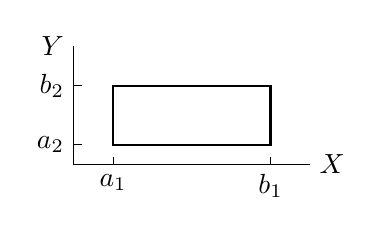
\begin{tikzpicture}
\draw(0,1.5)node[left]{$Y$}--(0,0)--(3,0)node[right]{$X$};
\draw[thick](0.5,0.25) rectangle (2.5,1);
\draw(0.5,0)node[below]{$a_1$}--++(0,0.1);
\draw(2.5,0)node[below]{$b_1$}--++(0,0.1);
\draw(0,0.25)node[left]{$a_2$}--++(0.1,0);
\draw(0,1)node[left]{$b_2$}--++(0.1,0);
\end{tikzpicture}
\caption{دو بعدی تقسیم کا تصور}
\label{شکل_شماریات_دو_بعدی_تقسیم}
\end{figure}

%==================
\جزوحصہء{غیر مسلسل دو بعدی تقسیمیں}
اگر \عددی{(X,Y)} درج ذیل خواص رکھتا ہو تب متغیر \عددی{(X,Y)} اور اس کا مطابقتی تقسیم \اصطلاح{غیر مسلسل}\فرہنگ{غیر مسلسل!تقسیم}\فرہنگ{غیر مسلسل!متغیر}\فرہنگ{discrete!variable}\فرہنگ{discrete!distribution} کہلائے گا۔

\عددی{X,Y} متناہی تعداد یا قابل شمار لامتناہی تعداد کی جوڑی قیمتیں \عددی{(x,y)} اختیار کر سکتا ہے جن کے مطابقتی احتمال مثبت ہوں گے۔ہر ایسا دائرہ کار جس میں ایسی کوئی جوڑی نہ پائی جاتی ہو کا احتمال \عددی{0} ہو گا\حاشیہد{دھیان رہے کہ پہلی خاصیت سے یہ نہیں کہا جا سکتا ہے}۔ 

فرض کریں کہ \عددی{x_i,y_j} ایسی کوئی  جوڑی ہے اور \عددی{P(X=x_i,Y=y_j)=p_{ij}} ہے(جہاں ہم فرض کرتے ہیں کہ \عددی{p_{ij}} کسی مخصوص \عددی{i,j} کی جوڑیوں  کے لئے صفر بھی ہو سکتا ہے)۔ تفاعل
\begin{align}
f(x,y)=
\begin{cases}
p_{ij}& x=x_i,y=y_j\\
0&\text{ورنہ}
\end{cases}
\end{align}
کو \عددی{(X,Y)} کا \اصطلاح{تفاعل احتمال} کہتے ہیں؛ یہاں غیر تابع طور پر \عددی{i=1,2,\cdots} اور \عددی{j=1,2,\cdots} ہیں۔مساوات \حوالہ{مساوات_شماریات_غیر_مسلسل_متغیر_ج} کا مماثل 
\begin{align}
F(x,y)=\sum_{x_i\le x}\sum_{y_j\le y}f(x_i,y_j)
\end{align}
ہے اور مساوات \حوالہ{مساوات_شماریات_غیر_مسلسل_متغیر_پ} کی جگہ درج ذیل شرط ہو گا۔
\begin{align}
\sum_{i}\sum_{j}f(x_i,y_j)=1
\end{align}

مثال کے طور پر اگر ہم ایک روپیہ اور پانچ روپیہ کے سکے اچھال کر 
\begin{align*}
X&=\text{\RL{ایک روپیہ کی خط کی تعداد}}\\
Y&=\text{\RL{پانچ روپیہ کی خط کی تعداد}}
\end{align*}
پر غور کریں تب \عددی{X} اور \عددی{Y} کی قیمت\عددی{0} یا \عددی{1} ہو سکتی ہے اور تفاعل احتمال
\begin{align*}
\text{\RL{ہو گا۔}}\,\, f(x,y)=0\,\,\text{\RL{ورنہ (ان کے علاوہ)}}\,\,f(0,0)=f(1,0)=f(0,1)=f(1,1)=\frac{1}{4}
\end{align*}

%======================
\جزوحصہء{استمراری دو بعدی تقسیمیں}
\عددی{(X,Y)} اور اس کا تقسیم اس صورت استمراری کہلاتے ہیں جب  مطابقتی تفاعل تقسیم کو دوہرا تکمل
\begin{align}
F(x,y)=\int_{-\infty}^{y}\int_{-\infty}^{x}f(x^*,y^*)\dif x^*\dif y^*
\end{align}
کی صورت میں لکھنا ممکن ہو جہاں \عددی{f(x,y)} معین، غیر منفی اور پورے مستوی میں محدود ہے ماسوائے متناہی تعداد کے استمراری قابل تفرق منحنیات پر۔ \عددی{f(x,y)} کو تقسیم کی \اصطلاح{کثافت احتمال} کہتے ہیں۔یوں درج ذیل ہو گا۔
\begin{align}
P(a_1<X\le b_1, a_2<Y\le b_2)=\int_{a_2}^{b_2}\int_{a_1}^{b_1}f(x,y)\dif x\dif y
\end{align}

مثال کے طور پر  (شکل \حوالہ{شکل_شماریات_یکساں_تقسیم_الف})
\begin{align}\label{مساوات_شماریات_یکساں_متعدد_متغیرات_کثافت}
f(x,y)=0\,\text{ورنہ}\,f(x,y)=\frac{1}{k}\,\text{میں ہو تب}\,R\,\text{\RL{مستطیل}} \,(x,y)\,\text{جب}
\end{align}
مستطیل \عددی{R} میں یکساں تقسیم کو ظاہر کرتا ہے؛ یہاں \عددی{k} مستطیل کا رقبہ یعنی \عددی{k=(\beta_1-\alpha_1)(\beta_2-\alpha_2)} ہے۔اس تقسیم کو شکل \حوالہ{شکل_شماریات_یکساں_تقسیم_ب} میں دکھایا گیا ہے۔
\begin{figure}
\centering
\begin{minipage}{0.45\textwidth}
\centering
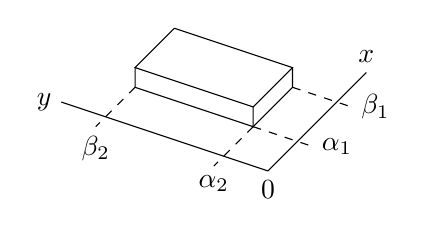
\begin{tikzpicture}[x={(-0.5cm,-0.5cm)},y={(0.75cm,-0.25cm)},z={(0,1cm)}]
\draw(0,0,0.25)--++(1,0,0)--++(0,2,0)--++(-1,0,0)--++(0,-2,0);
\draw(1,0,0.25)--++(0,0,-0.25)--++(0,2,0)--++(0,0,0.25);
\draw(1,2,0)--++(-1,0,0)--++(0,0,0.25);
\draw[dashed] (1,0,0)--++(1,0,0)node[below]{$\beta_2$};
\draw[dashed] (1,2,0)--++(1,0,0)node[below]{$\alpha_2$};
\draw[dashed](0,2,0)--++(0,1,0)node[right]{$\beta_1$};
\draw[dashed](1,2,0)--++(0,1,0)node[right]{$\alpha_1$};
\draw (1.75,2.75)node[below]{$0$}--++(-2.5,0,0)node[above]{$x$};
\draw (1.75,2.75)--++(0,-3.5,0)node[left]{$y$};
\end{tikzpicture}
\caption{یکساں تقسیم (مساوات \حوالہ{مساوات_شماریات_یکساں_متعدد_متغیرات_کثافت}) کا تفاعل احتمال کثافت}
\label{شکل_شماریات_یکساں_تقسیم_الف}
\end{minipage}\hfill
\begin{minipage}{0.45\textwidth}
\centering
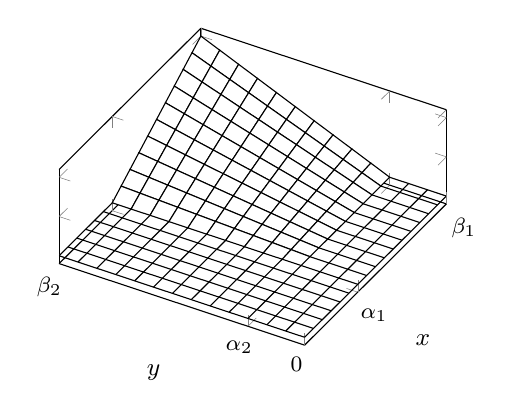
\begin{tikzpicture}
\begin{axis}[small, view={-60}{60},xtick={0.6,1.6},ytick={0,0.6,2.6},xticklabels={$\alpha_1$,$\beta_1$},yticklabels={$0$,$\alpha_2$,$\beta_2$},zticklabels={\empty},xlabel={$x$},ylabel={$y$}]
\addplot3[samples=11,samples y=11,surf,color=white,faceted color=black,domain=0.6:1.6,y domain=0.6:2.6]{(x-0.6)*(y-0.6)};
%the following manually matches the grid lines
\foreach \kk in {0.6,0.8,...,2.6}{
\addplot3 [domain=0:0.6, samples y=1, black,smooth] (x,\kk,0);}
\foreach \kk in {0.6,0.7,...,1.6}{
\addplot3 [domain=0:0.6, samples y=1, black,smooth] (\kk,x,0);}
\foreach \kk in {0,0.2,...,0.58}{
\addplot3 [domain=0:1.6, samples y=1, black,smooth] (x,\kk,0);}
\foreach \kk in {0,0.1,...,0.59}{
\addplot3 [domain=0:2.6, samples y=1, black,smooth] (\kk,x,0);}
\end{axis}
\end{tikzpicture}
\caption{یکساں تقسیم (مساوات \حوالہ{مساوات_شماریات_یکساں_متعدد_متغیرات_کثافت}) کا تفاعل تقسیم}
\label{شکل_شماریات_یکساں_تقسیم_ب}
\end{minipage}%
\end{figure}

%=================
\جزوحصہء{دو بعدی غیر مسلسل تقسیم کے حاشیہ تقسیمیں}
فرض کریں کہ بلا منصوبہ غیر مسلسل متغیر \عددی{(X,Y)} کا تفاعل احتمال \عددی{f(x,y)} ہے۔اگر \عددی{X=x} ہو، جبکہ \عددی{Y} جس میں ہمیں دلچسپی نہیں ہے کوئی بھی قیمت اختیار کر سکتا ہو، تب تفاعل احتمال \عددی{P(X=x,Y \text{اختیاری})} کو \عددی{f_1(x)} لکھا جا سکتا ہے جو \عددی{x} کا تابع تفاعل ہے۔یوں 
\begin{align}\label{مساوات_شماریات_حاشیہ_الف}
f_1(x)=P(X=x,Y\,\text{اختیاری})=\sum_y f(x,y)
\end{align} 
لکھا جا سکتا ہے جہاں اس \عددی{x} کے لئے ہم \عددی{f(x,y)} کی  تمام غیر صفر قیمتوں کا مجموعہ لیا گیا ہے۔ظاہر ہے کہ \عددی{f_1(x)} ایک بلا منصوبہ متغیر تقسیمی احتمال کا تفاعل احتمال ہے۔اس تقسیم کو دیے گئے دو بعدی تقسیم کے لحاظ ہے \عددی{X} کا \اصطلاح{حاشیہ تقسیم}\فرہنگ{تقسیم!حاشیہ}\حاشیہب{marginal distribution}\فرہنگ{distribution!marginal} کہا جاتا ہے۔اس کا تفاعل تقسیم درج ذیل ہو گا۔
\begin{align}\label{مساوات_شماریات_حاشیہ_ب}
F_1(x)=P(X\le x,Y\, \text{اختیاری})=\sum_{x^*\le x} f_1(x^*)
\end{align}
اسی طرح تفاعل احتمال 
\begin{align}\label{مساوات_شماریات_حاشیہ_پ}
f_2(y)=P(X\,\text{اختیاری}, Y=y)=\sum_x f(x,y))
\end{align}
دیے گیے دو بعدی تقسیم کا \عددی{Y} کے لحاظ سے \اصطلاح{حاشیہ تقسیم} تعین کرتا ہے۔مساوات \حوالہ{مساوات_شماریات_حاشیہ_پ} میں ہم \عددی{y} کے مطابقتی غیر صفر \عددی{f(x,y)} کا مجموعہ لیتے ہیں۔اس تقسیم کا تفاعل تقسیم درج ذیل ہو گا۔
\begin{align}
F_2(y)=P(X\,\text{اختیاری},Y\le y)=\sum_{y^*\le y}f_2(y^*)
\end{align}
ظاہر ہے کہ بلا منصوبہ متغیر \عددی{(X,Y)} کے دونوں حاشیہ تقسیم  غیر مسلسل ہیں۔

جدول \حوالہ{جدول_شماریات_تاش_ملکہ_بادشاہ} میں ان کی مثال دی گئی ہے جہاں تاش کے پتوں سے تین پتے نکال کر واپس رکھے جاتے ہیں۔ملکہ کے حصول کو \عددی{X} جبکہ بادشاہ کے حصول کو \عددی{Y} سے ظاہر کیا گیا ہے۔تاش کے کل \عددی{52} پتے ہوتے ہیں جن میں \عددی{4} ملکہ اور \عددی{4} بادشاہ کے پتے ہوتے ہیں۔یوں ایک پتہ نکال کر ملکہ حاصل کرنے کا احتمال \عددی{\tfrac{4}{52}=\tfrac{1}{13}} ہو گا۔یوں ایک پتہ نکال کر ملکہ یا بادشاہ حاصل کرنے کا احتمال \عددی{\tfrac{2}{13}} ہو گا۔اس طرح اس بلا منصوبہ تجربہ کا مطابقتی تفاعل احتمال
\begin{align*}
f(x,y)=\frac{3!}{x!y!(3-x-y)!}\big(\frac{1}{13}\big)^x\big(\frac{2}{13}\big)^y\big(\frac{10}{13}\big)^{3-x-y}\quad \quad (x+y\le 3)
\end{align*}
ہو گا اور ان کے علاوہ \عددی{f(x,y)=0} ہو گا۔جدول \حوالہ{جدول_شماریات_تاش_ملکہ_بادشاہ} میں \عددی{f(x,y)}، \عددی{f_1(x)} اور \عددی{f_2(y)} دیے گئے ہیں۔ 
\begin{table}
\caption{تاش سے ملکہ اور بادشاہ کا حصول}
\label{جدول_شماریات_تاش_ملکہ_بادشاہ}
\centering
\begin{otherlanguage}{english}
\begin{tabular}{C|CCCC||C}
\phantom{xxx}y&\multirow{2}{*}{0}&\multirow{2}{*}{1}&\multirow{2}{*}{2}&\multirow{2}{*}{3}&\multirow{2}{*}{$f_1(x)$}\\
x\phantom{xxx}&&&&&\\
\hline\Tstrut
0&\frac{1000}{2197}&\frac{600}{2197}&\frac{120}{2197}&\frac{8}{2197}&\frac{1728}{2197}\\  \Tstrut \Bstrut \Tstrut \Bstrut
1&\frac{300}{2197}&\frac{120}{2197}&\frac{12}{2197}&0&\frac{432}{2197}\\   \Tstrut \Bstrut   \Tstrut \Bstrut
2&\frac{30}{2197}&\frac{6}{2197}&0&0&\frac{36}{2197}\\   \Tstrut \Bstrut   \Tstrut \Bstrut
3&\frac{1}{2197}&0&0&0&\frac{1}{2197}\\ 
\hline
\hline   \Tstrut \Bstrut
f_2(y)&\frac{1331}{2197}&\frac{726}{2197}&\frac{132}{2197}&\frac{8}{2197}&\\  
\hline
\end{tabular}
\end{otherlanguage}
\end{table}

\جزوحصہء{دو بعدی استمراری تقسیم کے حاشیہ تقسیمیں}
اسی طرح کثافت \عددی{f(x,y)} والے  استمراری متغیر \عددی{X,Y} کے لئے ہم 
\begin{align*}
(X\le x, Y\,\text{اختیاری})\quad \text{یا}\quad (X\le x, -\infty <Y<\infty)
\end{align*}
پر غور کر سکتے ہیں جس کا مطابقتی احتمال
\begin{align*}
F_1(x)=P(X\le x, -\infty<Y<\infty)=\int_{-\infty}^{\infty} \big(\int_{-\infty}^{\infty} f(x^*,y)\dif y\big)\dif x^*
\end{align*}
ہو گا جس میں
\begin{align}
f_1(x)=\int_{-\infty}^{\infty} f(x,y)\dif y
\end{align}
لکھتے ہوئے
\begin{align}
F_1(x)=\int_{-\infty}^{\infty} f_1(x^*)\dif x^*
\end{align}
لکھا جا سکتا ہے۔\عددی{f_1(x)}  اور \عددی{F_1(x)} کو بالترتیب دیے گئے استمراری تقسیم کے لحاظ سے حاشیہ تقسیم \عددی{X} کی  \ترچھا{کثافت} اور \ترچھا{تقسیمی تفاعل} کہتے ہیں۔دیے گئے دو بعدی استمراری تقسیم کے لحاظ سے تفاعل
\begin{align}
f_2(y)=\int_{-\infty}^{\infty} f(x,y)\dif x
\end{align}
کو حاشیہ تقسیم \عددی{Y} کی کثافت اور
\begin{align}
F_2(y)=\int_{-\infty}^{\infty} f_2(y^*)\dif y^*=\int_{-\infty}^{\infty}\int_{-\infty}^{\infty} f(x,y^*)\dif x\dif y^*
\end{align}
کو حاشیہ تقسیم \عددی{Y} کا تقسیمی تفاعل کہتے ہیں۔ہم دیکھتے ہیں کہ استمراری تقسیم کے دونوں حاشیہ تقسیم استمراری ہیں۔

\جزوحصہء{بلا منصوبہ متغیرات کی تابعیت اور غیر تابعیت}
دو بعدی \عددی{(X,Y)} تقسیم جس کا تفاعل تقسیم \عددی{F(x,y)} ہو کے بلا منصوبہ متغیرات \عددی{X} اور \عددی{Y} اس صورت \اصطلاح{غیر تابع}\فرہنگ{تابع!غیر}\فرہنگ{independent} کہلاتے ہیں جب تمام \عددی{(x,y)} کے لئے
\begin{align}
F(x,y)=F_1(x)F_2(y)
\end{align}
ہو ورنہ انہیں \اصطلاح{تابع}\فرہنگ{تابع}\فرہنگ{dependent} کہتے ہیں۔


فرض کریں کہ \عددی{X} اور \عددی{Y} دونوں غیر مسلسل  یا دونوں استمراری ہوں۔تب \عددی{X} اور \عددی{Y} اس صورت غیر تابع ہوں گے جب ان کے مطابقتی تفاعل احتمال یا کثافتیں \عددی{f_1(x)} اور \عددی{f_2(y)} درج ذیل کو مطمئن کرتے ہوں (سوال \حوالہ{سوال_شماریات_غیر_تابعیت_ثبوت})۔
\begin{align}\label{مساوات_شماریات_تابعیت_غیر_تابعیت}
f(x,y)=f_1(x)f_2(y)
\end{align}
مثال کے طور پر جدول \حوالہ{جدول_شماریات_تاش_ملکہ_بادشاہ} میں متغیرات تابع ہیں۔ایک روپیہ اور پانچ روپیہ کے سکے ایک بار  اچھال کر متغیرات
\begin{align*}
X=\text{\RL{ایک روپیہ کے سکے کے خط کی تعداد}},\quad Y=\text{\RL{پانچ روپیہ کے سکے کے خط کی تعداد}}
\end{align*}
\عددی{0} یا \عددی{1} قیمت اختیار کر سکتے ہیں اور یہ متغیرات غیر تابع ہیں۔

تابعیت اور غیر تابعیت کی تصور کو \عددی{n} بعدی تقسیم \عددی{X_1,\cdots,X_n} جس کا تفاعل احتمال
\begin{align*}
F(x_1,\cdots,x_n)=P(X_!\le x_1,\cdots X_n\le x_n)
\end{align*}
ہو کے \عددی{n} بلا منصوبہ متغیرات  تک وسعت دی جا سکتی ہے۔اگر تمام \عددی{x_1,\cdots,x_n} کے لئے
\begin{align}
F(x_1,\cdots,x_n)=F_1(x_1)F_2(x_2)\cdots F_n(n)
\end{align}
ہو جہاں \عددی{X_j} کے حاشیہ تقسیم کا تقسیمی تفاعل \عددی{F_j(x_j)} ہو، یعنی
\begin{align*}
F_j(x_j)=P(X_j\le x_j, X_k\, \text{اختیاری},\, k\ne j)
\end{align*}
تب یہ بلا منصوبہ متغیرات \اصطلاح{غیر تابع} کہلاتے ہیں ورنہ  ان متغیرات کو \اصطلاح{تابع} کہتے ہیں۔

\جزوحصہء{بلا منصوبہ متغیرات کے تفاعل}
فرض کریں کہ بلا منصوبہ متغیر \عددی{(X,Y)} کا تفاعل احتمال یا کثافت \عددی{f(x,y)} اور تقسیمی تفاعل \عددی{F(x,y)} ہیں اور فرض کریں کہ \عددی{g(x,y)} غیر مستقل استمراری تفاعل ہے جو تمام \عددی{(x,y)} پر معین ہے۔تب \عددی{Z=g(X,Y)} بھی بلا منصوبہ متغیر ہو گا۔مثال کے طور پر ہم دو پانسہ پھینکتے ہیں۔پہلے پانسہ عدد \عددی{X} اور دوسرا پانسہ عدد \عددی{Y} دیتا ہے۔ عدد \عددی{Z=X+Y} ان دونوں کا مجموعہ ہے (شکل \حوالہ{شکل_شماریات_تفاعل_تقسیم_ب})۔

اگر \عددی{(X_1,\cdots,X_n) بلا منصوبہ \عددی{n}} بعدی متغیر ہوا ور تمام \عددی{(x_1,\cdots,x_n)} پر  \عددی{g(x_1,\cdots,x_n)} معین غیر مستقل استمراری تفاعل ہو  تب \عددی{Z=g(X_1,\cdots,X_n)} بھی بلا منصوبہ متغیر ہو گا۔

غیر مسلسل بلا منصوبہ متغیر \عددی{(X,Y)} کی صورت میں ان تمام \عددی{f(x,y)} کا مجموعہ لیتے ہوئے جن کے لئے \عددی{g(x,y)} کی قیمت زیر غور \عددی{y} کے برابر ہو،  ہم \عددی{Z=g(X,Y)} کا تفاعل احتمال \عددی{f(z)} حاصل کر سکتے ہیں، یعنی:
\begin{align}
f(z)=P(Z=z)=\underset{g(x,y)=z}{\sum\sum} f(x,y)
\end{align}
\عددی{Z} کا تقسیمی تفاعل
\begin{align}
F(z)=P(Z\le z)=\underset{g(x,y)\le z}{\sum\sum} f(x,y)
\end{align}
ہے جہاں ہم ان \عددی{f(x,y)} کا مجموعہ لیا جائے گا جن کے لئے \عددی{g(x,y)\le z} ہو۔

بلا منصوبہ استمراری متغیر \عددی{(X,Y)} کے لئے اسی طرح
\begin{align}
F(z)=P(Z\le z) =\underset{g(x,y)\le z}{\int\int} f(x,y)\dif x\dif y
\end{align}
ہو گا جہاں ہر \عددی{z} کے لئے ہم \عددی{xy} مستوی میں خطہ \عددی{g(x,y)\le z} پر تکمل حاصل کرتے ہیں۔

\جزوحصہء{\عددی{g(X,Y)} کی حسابی توقع۔مجموعہ  اوسط اور تغیریت}
درج ذیل عدد کو \عددی{g(X,Y)} کی \اصطلاح{حسابی توقع}\فرہنگ{توقع!حسابی}\حاشیہب{mathematical expectation}\فرہنگ{expectation!mathematical} یا مختصراً \اصطلاح{توقع} کہتے ہیں۔
\begin{align}
E(g(X,Y))=
\begin{cases}
\sum\limits_x \sum\limits_y g(x,y)f(x,y)\quad\quad\quad\quad [(X,Y)\,\text{غیر مسلسل}]   \\[2ex]
\int\limits_{-\infty}^{\infty}\int\limits_{-\infty}^{\infty} g(x,y)f(x,y)\dif x\dif y\quad [(X,Y)\, \text{استمراری}]
\end{cases}
\end{align}
یہاں ہم فرض کرتے ہیں کہ دوہرا مجموعہ مطلق مرتکز ہے اور  \عددی{xy} مستوی پر \عددی{\abs{g(x,y)}f(x,y)} کا تکمل موجود ہے۔درج ذیل کلیہ کو سوال \حوالہ{سوال_شماریات_خطی_مجموعہ_کلیہ} کی طرز پر ثابت کیا جا سکتا ہے۔
\begin{align}\label{مساوات_شماریات_خطی_اوسط_عمومی}
E(ag(X,Y)+bh(X,Y))=aE(g(X,Y))+bE(h(X,Y))
\end{align} 
اس کے ایک مخصوص صورت \عددی{E(X+Y)=E(X)+E(Y)} ہے اور الکراجی ماخوذ سے  درج ذیل حاصل ہوتا ہے۔

%========================
\ابتدا{مسئلہ}\شناخت{مسئلہ_شماریات_مجموعہ_اوسط}\quad \موٹا{(مجموعہ اوسط)}\\
بلا منصوبہ متغیرات کے مجموعے کی اوسط (توقع) ان کے انفرادی اوسط کا مجموعہ ہو گا، یعنی:
\begin{align}
E(X_1+X_2,\cdots+X_n)=E(X_1)+E(X_2)+\cdots+E(X_n)
\end{align}
\انتہا{مسئلہ}
%======================

مزید درج ذیل با آسانی حاصل کیا جا سکتا ہے۔

%===============
\ابتدا{مسئلہ}\شناخت{مسئلہ_شماریات_اوسط_حاصل_ضرب}\quad \موٹا{اوسطوں کا حاصل ضرب}\\
\موٹا{غیر تابع} بلا منصوبہ متغیرات کے حاصل ضرب کی اوسط ان کے انفرادی اوسط کے حاصل ضرب کے برابر ہو گا، یعنی:
\begin{align}\label{مساوات_شماریات_حاصل_ضرب_اوسط}
E(X_1X_2\cdots X_n)=E(X_1)E(X_2)\cdots E(X_n)
\end{align}
\انتہا{مسئلہ}
%========================
\ابتدا{ثبوت}\quad
فرض کریں کہ \عددی{X} اور \عددی{Y} بلا منصوبہ متغیرات ہیں (جہاں دونوں غیر مسلسل یا دونوں استمراری ہیں)۔ تب \عددی{E(XY)=E(X)E(Y)} ہو گا۔ غیر مسلسل صورت میں 
\begin{align*}
E(XY)=\sum_x\sum_y xyf(x,y)=\sum_x xf_1(x)\sum_y y f_2(y)=E(X)E(Y)
\end{align*}
لکھا جا سکتا ہے  اور استمراری صورت میں بھی ثبوت اسی طرح کا ہے۔اس نتیجہ کو \عددی{n} غیر تابع متغیرات تک وسعت دینے سے  مساوات \حوالہ{مساوات_شماریات_حاصل_ضرب_اوسط} ثابت ہوتی ہے۔یوں ثبوت مکمل ہوتا  ہے۔
\انتہا{ثبوت}
%===========================
 
ہم اب تغیریت کے مجموعہ پر غور کرتے ہیں۔فرض کریں کہ \عددی{Z=X+Y} ہے اور \عددی{Z} کی اوسط \عددی{\mu} اور تغیریت \عددی{\sigma^{\,2}} ہے۔سوال \حوالہ{سوال_شماریات_تغیریت_دوسرا_کلیہ} سے درج ذیل لکھا جا سکتا ہے۔
\begin{align*}
\sigma^{\,2}=E([Z-\mu]^2)=E(Z^2)-[E(Z)]^2
\end{align*}
مساوات \حوالہ{مساوات_شماریات_خطی_اوسط_عمومی} سے  دائیں ہاتھ پہلے جزو کو
\begin{align*}
E(Z^2)=E(X^2+2XY+Y^2)=E(X^2)+2E(XY)+E(Y^2)
\end{align*}
لکھا جا سکتا ہے جبکہ دائیں ہاتھ دوسرے جزو کو مسئلہ \حوالہ{مسئلہ_شماریات_اوسط_حاصل_ضرب} کی مدد سے
\begin{align*}
[E(Z)]^2=[E(X)+E(Y)]^2=[E(X)]^2+2E(X)E(Y)+[E(Y)]^2
\end{align*}
لکھا جا سکتا ہے۔انہیں \عددی{\sigma^{\,2}} کے کلیہ میں پر کرتے ہوئے درج ذیل حاصل ہوتا ہے۔
\begin{align*}
\sigma^{\,2}&=E(X^2)-[E(X)]^2+E(Y^2)-[E(Y)]^2\\
&\quad +2[E(XY)-E(X)E(Y)]
\end{align*}
سوال \حوالہ{سوال_شماریات_تغیریت_دوسرا_کلیہ} سے ہم دیکھتے ہیں کہ دائیں ہاتھ پہلی لکیر پر دیا گیا تعلق \عددی{X} اور \عددی{Y} کی تغیریت کا مجموعہ ہے  جنہیں ہم  بالترتیب \عددی{\sigma_1^2} اور \عددی{\sigma_2^2} سے ظاہر کرتے ہیں۔دوسری لکیر پر مقدار
\begin{align}
\sigma_{XY}=E(XY)-E(X)E(Y)
\end{align}
کو \عددی{X} اور \عددی{Y} کی \اصطلاح{باہمی تغیریت}\فرہنگ{تغیریت!باہمی}\حاشیہب{covariance}\فرہنگ{covariance} کہتے ہیں۔اس طرح درج ذیل حاصل ہوتا ہے۔
\begin{align}
\sigma^{\,2}=\sigma_1^2+\sigma_2^2+2\sigma_{XY}
\end{align}
اگر \عددی{X} اور \عددی{Y} غیر تابع ہوں تب \عددی{E(XY)=E(X)E(Y)} لہٰذا \عددی{\sigma_{XY}=0}  اور
\begin{align}
\sigma^{\,2}=\sigma_1^2+\sigma_2^2
\end{align}
ہو گا۔دو سے زائد متغیرات تک وسعت دیتے ہوئے درج ذیل حاصل ہو گا۔

%=============================
\ابتدا{مسئلہ}\شناخت{مسئلہ_شماریات_تغیرات_کا_مجموعہ}\quad \موٹا{(تغیرات کا مجموعہ)}\\
\موٹا{غیر تابع} بلا منصوبہ متغیرات کے مجموعہ کی تغیریت ان متغیرات کے انفرادی تغیریت کے مجموعہ کے برابر ہو گا۔
\انتہا{مسئلہ}
%===========================

\حصہء{سوالات}

\ابتدا{سوال}\شناخت{سوال_شماریات_ایک_سے_زائد_ثبوت_ب}\quad
مساوات \حوالہ{مساوات_شماریات_ایک_سے_زائد_ب} کو ثابت کریں۔\\
جواب:\quad
 شکل \حوالہ{شکل_سوال_شماریات_ایک_سے_زائد_ثبوت_ب} میں \عددیء{(X,Y)}  احتمال \عددی{F(b_1,b_2)} کے ساتھ \عددی{A}، \عددی{B}، \عددی{C} یا \عددی{D} سے قیمت اختیار کر سکتا ہے، احتمال \عددی{F(a_1,b_2)} کے ساتھ \عددی{A} یا \عددی{C} سے قیمت اختیار کر سکتا ہے، احتمال \عددی{F(b_1,a_2)} کے ساتھ \عددی{C} یا \عددی{D} سے قیمت اختیار کر سکتا ہے، احتمال \عددی{F(a_1,a_2)} کے ساتھ \عددی{C} سے قیمت اختیار کر سکتا ہے لہٰذا \عددی{B} سے قیمت حاصل کرنے کا احتمال مساوات \حوالہ{مساوات_شماریات_ایک_سے_زائد_ب} کا دایاں ہاتھ دے گا۔ 
\begin{figure}
\centering
\begin{tikzpicture}
\draw(0,0)node[left]{$Y=b_2$}--++(4,0)--++(0,-2.5)node[below]{$X=b_1$};
\draw(0,-1)node[left]{$Y=a_2$}--++(4,0);
\draw(1.75,0)--++(0,-2.5)node[below]{$X=a_1$};
\draw(1,-0.5)node[]{$A$}  (3,-0.5)node[]{$B$} (1,-1.5)node[]{$C$}  (3,-1.5) node[]{$D$};
\end{tikzpicture}
\caption{شکل برائے سوال \حوالہ{سوال_شماریات_ایک_سے_زائد_ثبوت_ب}}
\label{شکل_سوال_شماریات_ایک_سے_زائد_ثبوت_ب}
\end{figure}
\انتہا{سوال}
%=====================
\ابتدا{سوال}\quad
شکل \حوالہ{شکل_شماریات_یکساں_تقسیم_الف} اور شکل \حوالہ{شکل_شماریات_یکساں_تقسیم_ب} میں دیے تقسیم کے حاشیہ تقسیم حاصل کریں۔
\انتہا{سوال}
%======================
\ابتدا{سوال}\quad
فرض کریں کہ \عددی{8\le x \le 12} اور \عددی{0\le y\le 2} میں \عددی{f(x,y)=k} جبکہ باقی جگہوں پر \عددی{f=0}۔ \عددی{k}، \عددی{P(X\le 11, 1\le Y\le 1.5)} اور \عددی{P(9\le X\le 12, Y\le 1)} تلاش کریں۔\\
جواب:\quad
$\tfrac{1}{8}, \tfrac{3}{16},\tfrac{3}{8}$
\انتہا{سوال}
%======================
\ابتدا{سوال}\quad
ایک کاغذ کی اوسط کمیت \عددی{\SI{10}{\gram}} اور معیاری انحراف \عددی{\SI{0.05}{\gram}} ہے۔ ایسی \عددی{\num{10000}} کاغذوں کی ڈھیر کی اوسط کمیت اور تغیریت کیا ہو گی؟  
\انتہا{سوال}
%=========================
\ابتدا{سوال}\quad
فرض کریں کہ \عددی{x>0}، \عددی{y>0} اور \عددی{x+y<3} میں \عددی{f(x,y)=k} جبکہ باقی جگہوں پر \عددی{f=0} ہے۔\عددی{k} تلاش کریں۔ \عددی{f(x,y)} ترسیم کریں۔ \عددی{P(X+Y\le 1)} اور \عددی{P(Y>X)}  تلاش کریں۔\\
جواب:\quad
$\tfrac{2}{9}, \tfrac{1}{9},\tfrac{1}{2}$
\انتہا{سوال}
%========================
\ابتدا{سوال}\quad 
ایک خالی ڈبے کی اوسط \عددی{\SI{2}{\kilo\gram}} اور معیاری انحراف \عددی{\SI{0.1}{\kilo\gram}} ہے۔اس ڈبے میں مال کی اوسط \عددی{\SI{75}{\kilo\gram}} اور تغیریت \عددی{\SI{0.8}{\kilo\gram}} ہے۔بھرے ڈبے کی اوسط اور معیاری انحراف کیا ہوں گے؟ 
\انتہا{سوال}
%=======================
\ابتدا{سوال}\quad
خطہ \عددی{0\le x\le 1}، \عددی{0\le y\le 1} میں  بلا منصوبہ متغیرات کی کثافتیں \عددی{f(x,y)=x+y} اور \عددی{g(x,y)=(x+\tfrac{1}{2})(y+\tfrac{1}{2})} ہیں۔دکھائیں کہ ان کی حاشیہ تقسیم ایک جیسی ہیں۔ 
\انتہا{سوال}
%==========================
\ابتدا{سوال}\quad
ایسی دو مختلف غیر مسلسل تقسیم کی مثال دیں جن کے حاشیہ تقسیم ایک جیسی ہوں۔
\انتہا{سوال}
%=========================
\ابتدا{سوال}\quad
چار گراریوں کو یوں یکجا کیا جاتا ہے کہ ان کے بیچ فاصلہ رہے۔گراریوں کے بیچ باریک چادر کی ٹکیا رکھ کر فاصل پیدا کیا جاتا ہے۔گراری کی موٹائی کی  اوسط   \عددی{\SI{5.020}{\centi\meter}} اور معیاری انحراف \عددی{\SI{0.003}{\centi\meter}} ہے جبکہ ٹکیا کی موٹائی کی  اوسط \عددی{\SI{0.040}{\centi\meter}} اور معیاری انحراف 
\عددی{\SI{0.002}{\centi\meter}} ہے۔بلا منصوبہ  \عددی{4} گراریوں اور \عددی{3}  ٹکیوں سے بنائی گئی پوری گراری  کی موٹائی کی اوسط اور معیاری انحراف کیا ہوں گے۔\\
جواب:\quad
$20.200, 0.007\,\text{تقریباً}$
\انتہا{سوال}
%==========================
\ابتدا{سوال}\quad
لوہے کی چادروں اور کاغذ کو تہہ در تہہ رکھ کر ٹرانسفارمر کا قالب بنایا جاتا ہے۔اگر لوہے کی چادر کی موٹائی کی اوسط \عددی{\SI{0.5}{\milli\meter}} اور معیاری انحراف \عددی{\SI{0.05}{\milli\meter}} ہو اور کاغذ کی موٹائی کی اوسط \عددی{\SI{0.05}{\milli\meter}} اور معیاری انحراف \عددی{\SI{0.02}{\milli\meter}} ہو تب \عددی{50} لوہے کی چادروں اور \عددی{49} کاغذوں سے بنائے گئے قالب کی موٹائی کی اوسط اور معیاری انحراف کیا ہوں گے؟ 
\انتہا{سوال}
%==========================
\ابتدا{سوال}\quad
خطہ \عددی{x^2+y^2<1} میں \عددی{(X,Y)}  کی کثافت \عددی{f(x,y)=k} ہے جبکہ اس خطہ کے باہر کثافت صفر ہے۔\عددی{k} تلاش کریں۔حاشیہ تقسیم کی کثافتیں تلاش کریں۔احتمال \عددی{P(X^2+Y^2<\tfrac{1}{2})} تلاش کریں۔\\
جواب:\quad
$k=\tfrac{1}{\pi}; f_1(x)=\tfrac{2}{\pi}\sqrt{1-x^2},f_2(y)=\tfrac{2}{\pi}\sqrt{1-y^2}, \SI{50}{\percent}$
\انتہا{سوال}
%============================
\ابتدا{سوال}\quad
ایک پنیا اور سوراخ کے قطر بالترتیب \عددی{X} سنٹی میٹر اور \عددی{Y} سنٹی میٹر ہیں۔فرض کریں کہ \عددی{(X,Y)} کی کثافت
\begin{align*}
f(x,y)=2500 \quad \text{\RL{ہو تب}}\quad 0.99<x<1.01, 1.00<y<1.02 \quad \text{\RL{اگر}}
\end{align*}
ہے ورنہ \عددی{f=0} ہے۔ حاشیہ تقسیمیں حاصل کریں۔ اس بات کا کیا احتمال ہے کہ بلا منصوبہ منتخب کردہ پنیا \عددی{1.00} سنٹی میٹر کی سوراخ میں ٹھیک بیٹھے گا؟
\انتہا{سوال}
%========================
\ابتدا{سوال}\شناخت{سوال_شماریات_حاشیہ_تقسیم_الف}\quad
خطہ \عددی{x\ge 0, y\ge 0} میں \عددی{(X,Y)} کی کثافت \عددی{f(x,y)=e^{-(x+y)}} ہے جبکہ باقی جگہوں پر \عددی{f=0} ہے۔ \عددی{P(X>Y)} تلاش کریں۔\\
جواب:\quad
$\SI{50}{\percent}$
\انتہا{سوال}
%===========================
\ابتدا{سوال}\quad
سوال \حوالہ{سوال_شماریات_حاشیہ_تقسیم_الف} میں حاشیہ تقسیم کی کثافتیں تلاش کریں۔
\انتہا{سوال}
%===========================
\ابتدا{سوال}\quad
ایک برقیاتی آلہ میں دو برقیاتی پرزے پائے جاتے ہیں۔فرض کریں کہ پہلا پرزہ \عددی{X} مہینوں تک اور دوسرا پرزہ \عددی{Y} مہینوں تک کام کر سکتا ہے۔فرض کریں کہ \عددی{(X,Y)} کی احتمال کثافت
\begin{align*}
f(x,y)=0.01e^{-0.1(x+y)}\quad\quad x>0,y>0
\end{align*}
جبکہ اس کے علاوہ \عددی{f=0} ہے۔ (الف) کیا \عددی{X} اور \عددی{Y} تابع ہیں؟ (ب) حاشیہ تقسیم کی کثافت تلاش کریں۔ (پ) پہلے پرزے کی زندگی \عددی{10} مہینے یا اس سے زیادہ ہونے کا احتمال کیا ہو گا؟\\
جواب:\quad
غیر تابع،  
$f_1(x)=0.1e^{-0.1x}, x>0; f_2(y)=0.1e^{-0.1y}, y>0; \SI{36.8}{\percent}$
ہے
\انتہا{سوال}
%=========================
\ابتدا{سوال}\شناخت{سوال_شماریات_غیر_تابعیت_ثبوت}\quad
مساوات \حوالہ{مساوات_شماریات_تابعیت_غیر_تابعیت} سے منسلک فقرہ ثابت کریں۔
\انتہا{سوال}
%=========================
\ابتدا{سوال}\quad
فرض کریں کہ \عددی{(X,Y)} کا تفاعل احتمال \عددی{f(0,0)=f(1,1)=\tfrac{1}{8}}، \عددی{f(0,1)=f(1,0)=\tfrac{3}{8}} ہے۔کیا \عددی{X} اور \عددی{Y} غیر تابع ہیں؟\\
جواب: جی نہیں
\انتہا{سوال}
%=======================
\ابتدا{سوال}\quad
مسئلہ \حوالہ{مسئلہ_شماریات_مجموعہ_اوسط} کو استعمال کرتے ہوئے ثنائی تقسیم کی اوسط \عددی{\mu} کا کلیہ  حاصل کریں۔
\انتہا{سوال}
%====================
\ابتدا{سوال}\quad
مسئلہ \حوالہ{مسئلہ_شماریات_تغیرات_کا_مجموعہ} کی مدد سے ثنائی تقسیم کی تغیریت \عددی{\sigma^{\,2}} کا کلیہ تلاش کریں۔
\انتہا{سوال}
%==========================
\ابتدا{سوال}\quad
مسئلہ \حوالہ{مسئلہ_شماریات_مجموعہ_اوسط}  کی مدد سے  بیش ہندسی تقسیم کی اوسط کا کلیہ  حاصل کریں۔کیا  مسئلہ \حوالہ{مسئلہ_شماریات_تغیرات_کا_مجموعہ} کی مدد سے اس تقسیم کی تغیریت کا کلیہ حاصل کیا جا سکتا ہے؟
\انتہا{سوال}
%=======================

\حصہ{بلا منصوبہ نمونہ بندی۔ بلا منصوبہ اعداد}
حصہ \حوالہ{حصہ_شماریات_نمونی_اوسط_نمونی_تغیریت} تا حصہ \حوالہ{حصہ_شماریات_ایک_سے_زائد_متغیرات_تقسیمیں} میں نظریہ احتمال پر غور کیا گیا۔اس باب کے باقی حصوں میں شماریات پر غور کیا جائے گا۔آبادی کے حسابی نمونے بنانے میں نظریہ شماریات مدد دیتا ہے۔شماریاتی تراکیب، جن پر غور کیا جائے گا،  نظریہ اور  حقیقی مشاہدوں  کے مابین تعلقات پیش کرتے ہیں۔یوں نمونہ بندی کے ذریعہ آبادی کے بارے میں نتائج حاصل کیے جا سکتے ہیں (شماریاتی رائے زنی؛ حصہ \حوالہ{حصہ_شماریات_نوعیت_اور_مقصد})۔

اب تک اتنا جاننا کافی تھا کہ آبادی کے نمونہ سے مراد آبادی سے اشیاء کا انتخاب ہے (حصہ \حوالہ{حصہ_شماریات_نوعیت_اور_مقصد} میں مثالیں) لیکن اب ہمیں اس تصور کی تعریف باریک بینی سے دینی ہو گی۔حقیقتاً کسی بھی آبادی سے نمونہ بندی کے ذریعہ معنی خیز نتائج حاصل کرنے کی خاطر ضروری ہے کہ نمونہ \اصطلاح{بلا منصوبہ انتخاب}\فرہنگ{بلا منصوبہ!انتخاب}\حاشیہب{random selection}\فرہنگ{random!selection} ہو، یعنی آبادی میں ہر چیز کا  منتخب ہو کر نمونے میں شامل ہونے  کے احتمال کی قیمت معلوم ہو۔یہ شرط ہر صورت (کم از کم تخمینی طور پر) پوری کرنا لازم ہے ورنہ حاصل نتائج مکمل طور پر بے معنی اور غلط ہو سکتے ہیں۔

لامتناہی نمونی فضا کی صورت میں نمونی قیمتیں \اصطلاح{غیر تابع} ہوں گی، یعنی، کسی بلا منصوبہ تجربہ کو \عددی{n} مرتبہ سرانجام دیتے ہوئے حاصل \عددی{n} بلا منصوبہ نمونی قیمتیں ایک دوسرے پر اثر انداز نہیں ہوں گی۔ عمومی آبادی سے حاصل نمونوں کے لئے یہ یقینی طور پر  درست ہے۔متناہی نمونی فضا کی صورت میں اگر ہم واپس رکھ کر نمونہ حاصل کریں تب نمونی قیمتیں غیر تابع ہوں گی؛ اگر ہم واپس نہ رکھ کر نمونہ حاصل کریں تب،  آبادی کی جسامت کے لحاظ سے نمونے کی جسامت چھوٹی رکھتے ہوئے (مثلاً \عددی{1000} کی آبادی سے \عددی{5} یا \عددی{10} کا نمونہ  لیتے ہوئے)، حاصل نمونی قیمتیں \ترچھا{عملاً} غیر تابع ہوں گی۔ اس کے برعکس اگر ہم بغیر واپس رکھتے ہوئے متناہی آبادی سے بڑے نمونے لیں تب تابعیت کا بہت زیادہ اثر پایا جائے گا۔

بلا منصوبہ انتخاب کی شرط پر پورا اترنا آسان نہیں ہے۔ کئی وجوہات نمونہ بندی کے عمل پر اثر انداز ہو سکتی ہیں۔مثال کے طور پر اگر ایک خریدار نے \عددی{80} کی  ڈھیر سے \عددی{10} کا انتخاب کر کے ڈھیر خریدنے یا نہ خریدنے  کا فیصلہ کرنا ہو  تب وہ طبعی طور پر ان \عددی{10} چیزوں کا انتخاب کس طرح کرے گا کہ \عددی{\binom{80}{10}} ممکنات میں سے ہر ایک کے منتخب ہونے کا احتمال ایک جیسا ہو؟

اس مسئلے کی حل کے لئے مختلف تراکیب تشکیل دی گئی ہیں۔ہم اب  ایک ایسے طریقہ کار پر غور کرتے ہیں جس کو عموماً استعمال کیا جاتا ہے۔

ہم اس ڈھیر کے اجزاء کو \عددی{1} تا \عددی{80} کے شمار سے ظاہر کرتے ہیں۔اس کے بعد ہم ضمیمہ \حوالہ{ضمیمہ_جدول} میں بلا منصوبہ اعداد کی جدول استعمال کرتے ہوئے \عددی{10} اجزاء چنتے ہیں۔بلا منصوبہ اعداد کے جدول کو ہم یوں استعمال کرتے ہیں کہ ہم پہلے \عددی{0} سے \عددی{99} کوئی صف بلا منصوبہ منتخب کرتے ہیں۔بلا منصوبہ صف منتخب کرنے کی خاطر ہم ایک سکہ کو \عددی{7} مرتبہ اچھال کر \عددی{7} ثنائی ہندسوں پر مبنی عدد حاصل کرتے ہیں جس میں خط کو \عددی{1} اور شیر کو \عددی{0} سے ظاہر کیا جاتا ہے۔یہ ثنائی عدد \عددی{0} تا \عددی{127} کو ظاہر کر سکتا ہے۔\عددی{99} سے بڑا عدد حاصل ہونے کی صورت میں عدد کو رد کرتے ہوئے سکہ دوبارہ \عددی{7} مرتبہ اچھالا جاتا ہے حتیٰ کہ ہمیں \عددی{0} تا \عددی{99} کوئی عدد حاصل ہو جو صف دے گا۔اس کے بعد اسی طرح ہم بلا منصوبہ \عددی{0} تا \عددی{9} قطار منتخب کرتے ہیں۔بلا منصوبہ قطار منتخب کرنے کی خاطر سکہ \عددی{4} مرتبہ اچھال کر \عددی{4} ثنائی ہندسوں کا عدد حاصل کیا جاتا ہے۔فرض کریں کہ صف کے لئے \عددی{0011010\, (=26)} اور قطار کے لئے \عددی{0111\, (=7)} حاصل ہو تب جدول کے \عددی{26} ویں صف اور \عددی{7} ویں قطار سے \عددی{44973} حاصل کرتے ہوئے اس کے پہلے دو ہندسوں پر مبنی عدد \عددی{44} لیا جاتا ہے جبکہ باقی ہندسوں کو رد کیا جاتا ہے۔اسی قطر میں نیچے چلتے ہوئے اعداد کے پہلے دو ہندسے لیتے ہوئے درج ذیل اعداد حاصل کیے جاتے ہیں۔
\begin{align*}
44\quad 44\quad 83\quad 91\quad 55\quad \cdots
\end{align*}
ہم \عددی{80} سے بڑے اعداد رد کرتے ہیں اور کسی بھی عدد کو ایک سے زیادہ مرتبہ شامل نہیں کرتے ہیں۔یوں درکار بلا منصوبہ اعداد کا درج ذیل سلسلہ حاصل ہوتا ہے جس کے تحت اجزاء کو منتخب کیا جائے گا۔
\begin{align*}
44\quad 55\quad 53\quad 03\quad 52\quad 61\quad 67\quad 78\quad 39\quad 54
\end{align*}

زیادہ اجزاء کے نمونہ کے لئے  یہ طریقہ کار  موزوں نہیں ہے۔ اسی لئے  ایسے اعداد جن کی خاصیت بلا منصوبہ اعداد کی طرح ہو،  پیدا کرنے کے کئی طریقے بنائے گئے ہیں جنہیں کمپیوٹر کی زبان میں \اصطلاح{پیدا کار بلا منصوبہ اعداد}\فرہنگ{پیدا کار بلا منصوبہ اعداد}\حاشیہب{random number generator}\فرہنگ{random number generator} کہتے ہیں۔

\حصہء{سوالات}
%===================
\ابتدا{سوال}\quad
فرض کریں کہ مذکورہ بالا مثال میں ہم ضمیمہ \حوالہ{ضمیمہ_جدول} کے بلا منصوبہ اعداد کا جدول کے صف \عددی{83} اور قطار \عددی{2} سے شروع کرتے ہوئے اوپر رخ چلیں۔تب کون سے اجزاء نمونہ میں شامل کیے جائیں گے؟\\
جواب:\quad
$38,69,02,49,23,52,73,29,09,05$
\انتہا{سوال}
%========================
\ابتدا{سوال}\quad
ضمیمہ \حوالہ{ضمیمہ_جدول} کے بلا منصوبہ اعداد کا جدول استعمال کرتے ہوئے \عددی{250} کی ڈھیر سے \عددی{20} اجزاء بلا منصوبہ منتخب کریں۔
\انتہا{سوال}
%==========================
\ابتدا{سوال}\quad
منصفانہ پانسہ کو بلا منصوبہ انتخاب کے لئے کس طرح استعمال کیا جا سکتا ہے؟
\انتہا{سوال}
%=============================
\ابتدا{سوال}\شناخت{سوال_شماریات_نقل_اتارنا_الف}\quad
ایک بلا منصوبہ متغیر \عددی{Y} پر غور کریں جس کی خطہ \عددی{0<y<1} میں کثافت یکساں \عددی{f(y)=1}  جبکہ خطہ سے باہر \عددی{f=0} ہے۔ہم بلا منصوبہ اعداد کی مدد سے با آسانی \عددی{Y} (یعنی \عددی{Y} کی قیمتوں) کا \اصطلاح{نقل اتار}\فرہنگ{نقل اتارنا}\حاشیہب{simulation}\فرہنگ{simulation}  سکتے ہیں۔ مثال کے طور پر \عددی{2} اعشاریہ تک کے \عددی{20} قیمتیں حاصل کرنے کی خاطر ہم ضمیمہ \حوالہ{ضمیمہ_جدول} کے بلا منصوبہ اعداد کے جدول کے کسی بھی (بلا منصوبہ) قطار اور صف سے شروع کرتے ہوئے نیچے چلتے ہوئے، پانچ ہندسوں پر مشتمل دیے اعداد کے صرف پہلے دو ہندسوں کو لیتے ہوئے ان کے بائیں جانب اعشاریہ پر کرتے ہوئے اعداد حاصل کر سکتے ہیں۔ہم ایک سے زیادہ مرتبہ آنے والے اعداد کو بھی شامل کرتے ہیں۔فرض کریں ہم صف \عددی{36} اور قطار \عددی{3} سے شروع کرتے ہیں۔دکھائیں کہ درج ذیل حاصل ہو گا۔ان کا تعددی نقطہ ترسیم کھینچیں۔
\begin{align*}
0.89\quad 0.40\quad 0.67\quad 0.86\quad 0.87\quad 0.86\quad 0.06\quad 0.20\quad 0.38\quad 0.12\\
0.68\quad 0.50\quad 0.53\quad 0.10\quad 0.08\quad 0.90\quad 0.19\quad 0.85\quad 0.53\quad 0.98
\end{align*}
 \انتہا{سوال}
%=======================
\ابتدا{سوال}\شناخت{سوال_شماریات_نقل_اترنا_ب}\quad
بلا منصوبہ اعداد کی مدد سے کسی بھی بلا منصوبہ استمراری متغیر \عددی{X} کی نقل اتاری جا سکتی ہے۔ایسا کرنے کی خاطر ہم \عددی{X} کی تفاعل تقسیم کو ترسیم کرتے ہیں۔ سوال \حوالہ{سوال_شماریات_نقل_اتارنا_الف} کی طرز پر بلا منصوبہ اعداد کی مدد سے متغیر \عددی{Y} کی قیمتیں حاصل کرتے ہوئے انہیں \عددی{y} محدد پر ترسیم کریں اور ان کے مطابقتی \عددی{X} قیمتیں پڑھیں۔سوال \حوالہ{سوال_شماریات_نقل_اتارنا_الف} کی قیمتیں استعمال کرتے ہوئے عمومی بلا منصوبہ متغیر \عددی{X}، جس کی اوسط \عددی{0} اور تغیریت \عددی{1} ہو، کے لئے یہ طریقہ کار استعمال کریں۔جماعتی نشان \عددی{-2}، \عددی{-1}، \عددی{0}، \عددی{1} اور \عددی{2} لیتے ہوئے  \عددی{x} کی ان \عددی{20} نمونی قیمتوں کا مستطیلی ترسیم  کھینچیں۔\\
جواب:\quad
جماعتی تعدد \عددی{1}، \عددی{5}، \عددی{7}، \عددی{6}، \عددی{1} ہیں۔
\انتہا{سوال}
%========================
\ابتدا{سوال}\quad
سوال \حوالہ{سوال_شماریات_نقل_اترنا_ب} کا طریقہ کار غیر مسلسل بلا منصوبہ متغیر کے لئے  بھی قابل استعمال ہے۔اگر دو منصفانہ پانسہ پھینک کر حاصل اعداد کا مجموعہ \عددی{X} ہو تب اس طریقہ کو کس طرح استعمال کیا جائے گا؟
\انتہا{سوال}
%=======================

\حصہ{مقدار معلوم کا اندازہ لگانا}\شناخت{حصہ_شماریات_مقدار_معلوم_اندازہ_لگانا}
تقسیمات میں پائی جانے والے مقدار مثلاً ثنائی تقسیم میں \عددی{p}، عمومی تقسیم میں \عددی{\mu} اور \عددی{\sigma}، کو \اصطلاح{مقدار معلوم}\فرہنگ{مقدار معلوم}\حاشیہب{parameters}\فرہنگ{parameter} کہتے ہیں۔

ایک نقطہ پر مقدار معلوم کی اندازاً قیمت (\اصطلاح{نقطی اندازہ}\فرہنگ{اندازہ!نقطی}\حاشیہب{point estimate}\فرہنگ{estimate!point})  ایک عدد (حقیقی محور پر نقطہ) ہو گا جس کو دیے گئے نمونہ سے حاصل کیا جاتا ہے جو مقدار معلوم کی اصل قیمت کی تخمین ہو گی۔ \اصطلاح{وقفہ اندازہ}\فرہنگ{وقفہ!اندازہ}\حاشیہب{interval estimate}\فرہنگ{interval!estimate} (یعنی \ترچھا{وقفہ اعتماد}\فرہنگ{وقفہ!اعتماد}\حاشیہب{confidence interval}\فرہنگ{confidence interval})، جس پر اگلے حصے میں بحث کی جائے گی،  کو نمونہ سے حاصل کیا جاتا ہے۔مقدار معلوم کی قیمت کا اندازہ لگانا ایک اہم مسئلہ ہے۔

آبادی کی اوسط \عددی{\mu}  کا اندازہ لگانے کی خاطر ہم نمونے کی اوسط \عددی{\overline{x}} لے سکتے ہیں جس سے ہمیں \عددی{\mu} کا اندازہ \عددی{\widehat{\mu}=\overline{x}}  حاصل ہوتا ہے، یعنی
\begin{align}\label{مساوات_شماریات_اندازہ_الف}
\widehat{\mu}=\overline{x}=\frac{1}{n}(x_1+\cdots+x_n)
\end{align}
جہاں نمونہ کی جسامت \عددی{n} ہے۔اسی طرح آبادی کی تغیریت کا اندازہ \عددی{\widehat{\sigma^{\,2}}} در حقیقت مطابقتی نمونے کی تغیریت \عددی{s^2} ہو گی، یعنی:
\begin{align}\label{مساوات_شماریات_اندازہ_ب}
\widehat{\sigma^{\,2}}=s^2=\frac{1}{n-1}\sum_{j=1}^{n} (x_j-\overline{x})^2
\end{align}   
ظاہر ہے کہ مساوات \حوالہ{مساوات_شماریات_اندازہ_الف} اور مساوات \حوالہ{مساوات_شماریات_اندازہ_ب}  ان تقسیمات کی مقدار معلوم کی اندازاً قیمت دیتے ہیں جن میں \عددی{\mu} اور \عددی{\sigma^{2}} صریحاً پائے جاتے ہیں؛ عمومی تقسیم اور پوئسن تقسیم ایسی تقسیمات ہیں۔ثنائی تقسیم میں \عددی{p=\tfrac{\mu}{n}} (مساوات \حوالہ{مساوات_شماریات_ثنائی_تقسیم_پ}) ہے۔ اس صورت میں  اگر \عددی{j} ویں کوشش میں وقوعہ \عددی{A} جس کا احتمال \عددی{p} ہے واقع ہو تب مساوات \حوالہ{مساوات_شماریات_اندازہ_الف} میں \عددی{x_j=1} ہو گا اور اگر اس کوشش میں \عددی{A} واقع نہ ہو تب  \عددی{x_j=0} ہو گا۔ اس طرح مساوات \حوالہ{مساوات_شماریات_اندازہ_الف} سے \عددی{p} کا اندازہ درج ذیل حاصل ہو گا۔
\begin{align}
\widehat{p}=\frac{\overline{x}}{n}
\end{align}

ہم یہاں بتانا چاہتے ہیں کہ مساوات \حوالہ{مساوات_شماریات_اندازہ_الف} \اصطلاح{ترکیب معیار اثر}\فرہنگ{معیار اثر!ترکیب}\حاشیہب{method of moments}\فرہنگ{moments!method of} کی ایک مخصوص صورت ہے۔اس ترکیب میں جس مقدار معلوم کی اندازاً قیمت درکار ہو، اس کو تقسیم کی معیار اثر کی صورت میں لکھا جاتا ہے (حصہ \حوالہ{حصہ_شماریات_تقسیم_کا_اوسط_اور_تغیریت})۔حاصل کلیات میں ان معیار اثر کی جگہ نمونہ سے حاصل مطابقتی معیار اثر  پر کرتے ہوئے درکار اندازے حاصل کیے جاتے ہیں۔یہاں نمونہ \عددی{x_1,\cdots,x_n} کا \عددی{k} واں معیار اثر درج ذیل ہے۔
\begin{align*}
m_k=\frac{1}{n}\sum_{j=1}^{n}x_j^k
\end{align*}

اندازے حاصل کرنے کی دوسری ترکیب کو \اصطلاح{زیادہ سے زیادہ امکان کی ترکیب}\فرہنگ{ترکیب!زیادہ سے زیادہ امکان}\حاشیہب{maximum likelihood method}\فرہنگ{method!maximum likelihood} کہتے ہیں۔اس ترکیب کو سمجھنے کی خاطر ہم غیر مسلسل (یا استمراری) بلا منصوبہ متغیر \عددی{X} پر غور کرتے ہیں جس کا تفاعل احتمال واحد  متغیر \عددی{\theta} پر منحصر ہے۔ ہم \عددی{n} غیر تابع قیمتوں \عددی{x_1,\cdots,x_n} کا نمونہ لیتے ہیں۔تب غیر مسلسل صورت میں \عددی{n} جسامت کے نمونہ میں بالکل یہی قیمتیں حاصل ہونے کا احتمال درج ذیل ہو گا۔
\begin{align}\label{مساوات_شماریات_غیر_تابع_کا_احتمال}
l=f(x_1)f(x_2)\cdots f(x_n)
\end{align}
استمراری صورت میں،  چھوٹے چھوٹے وقفوں  \عددی{x_i\le x\le x_i+\Delta x\,\, (i=1,2,\cdots,n)} میں قیمتیں حاصل کرنے کا احتمال درج ذیل ہو گا۔
\begin{align}
f(x_1)\Delta x f(x_2)\Delta x\cdots f(x_n)\Delta x=l(\Delta x)^n
\end{align} 
چونکہ \عددی{f(x_i)} متغیر \عددی{\theta} کا تابع ہے لہٰذا تفاعل \عددی{l} متغیرات \عددی{x_1,\cdots,x_n} اور \عددی{\theta} کا تابع ہو گا۔ہم فرض کرتے ہیں کہ ہمیں \عددی{x_1,\cdots,\x_n} دیے گئے ہیں اور یہ مقررہ قیمتیں ہیں۔تب \عددی{l} متغیر \عددی{\theta} کا تابع ہو گا جس کو \اصطلاح{تفاعل امکان}\فرہنگ{تفاعل!امکان}\حاشیہب{likelihood function}\فرہنگ{function!likelihood} کہتے ہیں۔ زیادہ سے زیادہ امکان کی ترکیب کا بنیادی تصور بہت سادہ ہے۔ہم نا معلوم قیمت \عددی{\theta} کے لئے وہ تخمین چنتے ہیں جس سے \عددی{l} کی زیادہ سے زیادہ قیمت حاصل ہو۔اگر تفاعل \عددی{l} متغیر \عددی{\theta} کا قابل تفرق تفاعل ہو تب (سرحد سے ہٹ کر) \عددی{l} کی زیادہ سے زیادہ قیمت کے لئے درج ذیل  لازمی شرط ہے۔
\begin{align}\label{مساوات_شماریات_زیادہ_سے_زیادہ_الف}
\frac{\partial l}{\partial \theta}=0
\end{align}
(ہم یہاں جزوی تفرق لکھتے ہیں چونکہ \عددی{l} متغیرات \عددی{x_1,\cdots,x_n} کا بھی تابع ہے۔) مساوات \حوالہ{مساوات_شماریات_زیادہ_سے_زیادہ_الف} کا حل جو \عددی{x_1,\cdots,x_n} کا تابع ہے \عددی{\theta} کے  \ترچھا{زیادہ سے زیادہ امکان کا اندازہ} کہلاتا ہے۔چونکہ \عددی{f(x)\ge 0} اور \عددی{f(x)} کی زیادہ سے زیادہ قیمت عموماً مثبت ہوتی ہے اور  \عددی{\ln l} یک سر بڑھتا تفاعل ہے لہٰذا مساوات \حوالہ{مساوات_شماریات_زیادہ_سے_زیادہ_الف} کی جگہ درج ذیل بھی استعمال کیا جا سکتا ہے
\begin{align}\label{مساوات_شماریات_زیادہ_سے_زیادہ_ب}
\frac{\partial \ln l}{\partial \theta}=0
\end{align}
 جس سے عموماً حساب میں آسانی پیدا ہوتی ہے۔

اگر \عددی{X} کی تقسیم میں \عددی{r} مقدار معلوم \عددی{\theta_1,\cdots,\theta_r} پائے جاتے ہوں تب مساوات \حوالہ{مساوات_شماریات_زیادہ_سے_زیادہ_الف} کی جگہ \عددی{r} لازمی شرائط \عددی{\tfrac{\partial l}{\partial \theta_1}=0,\cdots,\tfrac{\partial l}{\partial \theta_r}=0} ہوں  گے اور مساوات \حوالہ{مساوات_شماریات_زیادہ_سے_زیادہ_ب} کی جگہ درج ذیل لکھا جائے گا۔ 
\begin{align}\label{مساوات_شماریات_زیادہ_سے_زیادہ_پ}
\frac{\partial \ln l}{\partial \theta_1}=0,\quad \cdots,\quad \frac{\partial \ln l}{\partial \theta_r}=0
\end{align}

%=====================
\ابتدا{مثال}\quad \موٹا{عمومی تقسیم}\\
عمومی تقسیم کی صورت میں \عددی{\mu} اور \عددی{\sigma} کی زیادہ سے زیادہ امکان کا اندازہ تلاش کریں۔\\
حل:\quad
مساوات \حوالہ{مساوات_شماریات_عمومی_تقسیم_الف} اور  مساوات \حوالہ{مساوات_شماریات_غیر_تابع_کا_احتمال} سے درج ذیل لکھا جا سکتا ہے۔
\begin{align*}
l=\big(\frac{1}{\sqrt{2\pi}}\big)^n \big(\frac{1}{\sigma}\big)^n e^{-h}\quad \quad h=\frac{1}{2\sigma^{\,2}}\sum_{i=1}^{n}(x_i-\mu)^2
\end{align*}
دونوں ہاتھ لوگارتھم لیتے ہیں۔
\begin{align*}
\ln l=-n\ln \sqrt{2\pi}-n\ln \sigma-h
\end{align*} 
مساوات \حوالہ{مساوات_شماریات_زیادہ_سے_زیادہ_پ} میں پہلی شرط \عددی{\tfrac{\partial \ln l}{\partial \mu}=0} ہے جس سے  درج ذیل لکھا جا سکتا ہے
\begin{align*}
\frac{\partial \ln l}{\partial \mu}=-\frac{\partial h}{\partial \mu}=\frac{1}{\sigma^2}\sum_{i=1}^{n}(x_i-\mu)=0\quad \implies \quad \sum_{i=1}^{n} x_i-n\mu=0
\end{align*}
جس کا حل \عددی{\mu} کا درکار اندازہ \عددی{\widehat{\mu}} ہے، یعنی:
\begin{align*}
\widehat{\mu}=\frac{1}{n}\sum_{i=1}^{n} x_i=\overline{x}
\end{align*} 
مساوات \حوالہ{مساوات_شماریات_زیادہ_سے_زیادہ_پ} میں دوسری شرط \عددی{\tfrac{\partial \ln l}{\partial \sigma}=0} ہے  جس سے  درج ذیل لکھا جا سکتا ہے۔
\begin{align*}
\frac{\partial \ln l}{\partial \sigma}=-\frac{n}{\sigma}-\frac{\partial h}{\partial \sigma}=-\frac{n}{\sigma}+\frac{1}{\sigma^3}\sum_{i=1}^{n} (x_i-\mu)^2=0
\end{align*}
\عددی{\mu} کی جگہ \عددی{\widehat{\mu}} پر کرتے ہوئے \عددی{\sigma^2} کے لئے حل کر کے درج ذیل ملتا ہے۔
\begin{align*}
\widetilde{\sigma}^{2}=\frac{1}{n}\sum_{i=1}^{n} (x-\overline{x})^2
\end{align*}
دھیان رہے کہ یہ نتیجہ مساوات \حوالہ{مساوات_شماریات_اندازہ_ب} سے مختلف ہے۔ہم اندازوں کی عمدگی کی قواعد پر بحث نہیں کر سکتے ہیں لیکن اتنا جاننا ضروری ہے کہ چھوٹی \عددی{n} کے لئے  مساوات \حوالہ{مساوات_شماریات_اندازہ_ب} بہتر نتائج دیتی ہے۔
\انتہا{مثال}
%====================

\حصہء{سوالات}
%================
\ابتدا{سوال}\شناخت{سوال_شماریات_اندازہ_الف}\quad 
\عددی{x\ge 0} کے لئے کثافت \عددی{f(x)=\theta e^{-\theta x}} اور \عددی{x<0} کے لئے \عددی{f(x)=0} ہے۔\عددی{\theta} کی زیادہ سے زیادہ امکان کا اندازہ حاصل کریں۔\\
جواب:\quad
$\widehat{\theta}=\tfrac{n}{\sum x_j}=\tfrac{1}{\overline{x}}$
\انتہا{سوال}
%==================
\ابتدا{سوال}\quad
سوال \حوالہ{سوال_شماریات_اندازہ_الف} میں اوسط \عددی{\mu} تلاش کر کے  \عددی{f(x)} میں پر کریں۔\عددی{\mu} کے زیادہ سے زیادہ امکان کا اندازہ حاصل کرتے ہوئے دکھائیں کہ یہ وہی ہے جو سوال \حوالہ{سوال_شماریات_اندازہ_الف} کے  \عددی{\theta} کے اندازے  سے حاصل کیا جا سکتا ہے۔ 
\انتہا{سوال}
%======================
\ابتدا{سوال}\quad
معلوم  تغیریت \عددی{\sigma^2=\sigma_0^2} کی عمومی تقسیم کے \عددی{\mu} کی زیادہ سے زیادہ امکان کا اندازہ حاصل کریں۔\\
جواب:\quad
$\widehat{\mu}=\overline{x}$
\انتہا{سوال}
%====================
\ابتدا{سوال}\quad
\عددی{\mu=0} کی صورت میں عمومی تقسیم پر زیادہ سے زیادہ امکان کے اندازے کی ترکیب لاگو کریں۔
\انتہا{سوال}
%======================
\ابتدا{سوال}\quad \موٹا{(پوئسن تقسیم)} \quad
زیادہ سے زیادہ امکان کے اندازہ کی ترکیب کا اطلاق  تقسیم پوئسن پر کریں۔ \\
جواب:\quad
$\widehat{\mu}=\overline{x}$
\انتہا{سوال}
%=================
\ابتدا{سوال}\quad \موٹا{(یکساں تقسیم)}  \quad
حصہ \حوالہ{حصہ_شماریات_تقسیم_کا_اوسط_اور_تغیریت} میں دیے گئے یکساں تقسیم کی صورت میں دکھائیں کہ مقدار معلوم \عددی{a} اور \عددی{b} کو زیادہ سے زیادہ امکان کا اندازہ استعمال کرتے ہوئے پہلی جزوی تفرق کو صفر کے برابر پر نہیں کیا جا سکتا ہے۔اس صورت میں زیادہ سے زیادہ امکان کا اندازہ کس طرح لگایا جا سکتا ہے؟
\انتہا{سوال}
%=====================
\ابتدا{سوال}\شناخت{سوال_شماریات_ثنائی_زیادہ_سے_زیادہ}\quad \موٹا{(ثنائی تقسیم)} \quad
\عددی{p} کے لئے زیادہ سے زیادہ امکان کا اندازہ حاصل کریں۔\\
جواب:\quad
$l=p^k(1-p)^{n-k}, \widehat{p}=\tfrac{k}{n}, k=\text{\RL{کوششوں میں کامیابی کی تعداد}}\, n$
\انتہا{سوال}
%========================
\ابتدا{سوال}\شناخت{سوال_شماریات_واحد_وقوعہ_الف}\quad
وقوعہ \عددی{A} واقع ہونے تک کوششوں کی تعداد \عددی{X} ہے۔دکھائیں کہ \عددی{X} کا تفاعل احتمال \عددی{f(x)=pq^{x-1},\,x=1,2,\cdots} ہے جہاں واحد کوشش میں \عددی{A} واقع ہونے کا احتمال \عددی{p} ہے اور \عددی{q=1-p} ہے۔\عددی{X} کی واحد قیمت \عددی{x} کے مشاہدے میں \عددی{p} کا زیادہ سے زیادہ امکان کا اندازہ تلاش کریں۔
\انتہا{سوال}
%=====================
\ابتدا{سوال}\quad
سوال \حوالہ{سوال_شماریات_واحد_وقوعہ_الف} میں نمونہ \عددی{x_1,\cdots,x_n} سے \عددی{p} کا زیادہ سے زیادہ امکان کا اندازہ حاصل کریں۔\\
جواب:\quad
$\widehat{p}=\frac{1}{\overline{x}}$
\انتہا{سوال}
%==========================
\ابتدا{سوال}\quad
سوال \حوالہ{سوال_شماریات_ثنائی_زیادہ_سے_زیادہ}  کو وسعت دیتے ہیں۔فرض کریں کہ \عددی{n} کوششوں کو \عددی{m} مرتبہ دہرایا جاتا ہے۔پہلی \عددی{n} کوششوں میں \عددی{A} واقع ہونے کی تعداد \عددی{k_1} ہے، دوسری \عددی{n} کوششوں میں \عددی{A} واقع ہونے کی تعداد \عددی{k_2} ہے، \نقطے، \عددی{m} ویں \عددی{n} کوششوں میں \عددی{A} واقع ہونے کی تعداد \عددی{k_m} ہے۔ان معلومات سے \عددی{p} کا زیادہ سے زیادہ امکان کا اندازہ حاصل کریں۔
\انتہا{سوال}
%======================

\حصہ{وقفہ اعتماد}
گزشتہ حصہ میں مقدار معلوم کی نقطی اندازہ پر غور کیا گیا۔اب ہم \اصطلاح{وقفی اندازہ}\فرہنگ{اندازہ!وقفی}\حاشیہب{interval estimate}\فرہنگ{estimate!interval} پر غور کریں گے۔

حسابی تخمینی کلیات استعمال کرتے ہوئے ضروری ہے کہ ہم جاننے کی کوشش کریں کہ  تخمینی قیمت اور اصل درست قیمت میں کتنا فرق ہے۔مثال کے طور پر اعدادی تکملی تراکیب میں زیادہ سے زیادہ خلل کے کلیات پائے جاتے ہیں جس سے ہم جان سکتے ہیں کہ تخمینی قیمت اور  اصل قیمت میں کتنا فرق پایا جا سکتا ہے۔فرض کریں کہ ہم کسی تکمل کا اعدادی تخمینی قیمت \عددی{2.47}  اور اصل قیمت سے زیادہ سے زیادہ ممکنہ خلل \عددی{\mp 0.02} حاصل کریں۔تب ہم پوری یقین کے ساتھ کہہ سکتے ہیں کہ تکمل کی اصل قیمت \عددی{2.47-0.02=2.45} تا  \عددی{2.47+0.02=2.49} قیمتوں میں \ترچھا{شامل} ہے، یعنی اصل قیمت  \عددی{2.47-0.02=2.45} یا اس سے زیادہ اور  \عددی{2.47+0.02=2.49} یا اس سے کم ہو گی۔

مقدار معلوم \عددی{\theta} کا اندازہ  لگاتے ہوئے ہم نمونی قیمتوں پر منحصر ایسے دو مقدار جاننا چاہیں گے جن میں یقینی طور پر اصل قیمت شامل ہو۔البتہ ہم جانتے ہیں کہ نمونی قیمتوں سے  \عددی{\SI{100}{\percent}} درست نتائج حاصل کرنا ممکن نہیں ہے۔یوں حقیقت پسندی سے کام  لیتے ہوئے ہم اس مسئلے کو درج ذیل بیان کرتے ہیں۔

احتمال \عددی{\gamma} کی قیمت کو \عددی{1} کے قریب منتخب کریں (مثلاً، \عددی{\gamma=\SI{95}{\percent}} یا \عددی{\gamma=\SI{99}{\percent}}، وغیرہ)۔ اس کے بعد ایسے  دو مقدار \عددی{\Theta_1} اور \عددی{\Theta_2} منتخب کریں جن میں مقدار معلوم \عددی{\theta} کی اصل قیمت کے شامل ہونے کا احتمال \عددی{\gamma} ہو۔

ہم سو فی صد یقین کے ساتھ جاننے کی "نا ممکن شرط" کی بجائے تقریباً \عددی{1} احتمال کی "ممکن شرط" پیش کرتے ہیں۔

دیے گئے نمونہ \عددی{x_1,\cdots,x_n} سے ان دو مقداروں کی قیمتوں کا حساب لگایا جائے گا۔ان \عددی{n} قیمتوں کو مشاہدے سے حاصل \عددی{n} بلا منصوبہ متغیرات \عددی{X_1,\cdots,X_n} کی قیمتیں تصور کریں۔تب \عددی{\Theta_1} اور \عددی{\Theta_2} ان بلا منصوبہ متغیرات کے تفاعل ہوں گے اور یوں خود بھی بلا منصوبہ متغیرات ہوں گے۔اس طرح ہماری شرط درج ذیل لکھی جا سکتی ہے۔
\begin{align*}
P(\Theta_1\le \theta \le \Theta_2)=\gamma
\end{align*}
اگر ہمیں تفاعل \عددی{\Theta_1} اور \عددی{\Theta_2} معلوم ہوں، تب دیے گئے نمونہ سے ہم \عددی{\Theta_1} کی  اعدادی قیمت \عددی{\theta_1} اور \عددی{\Theta_2} کی اعدادی قیمت \عددی{\theta_2} کا حساب لگا سکتے ہیں۔وہ وقفہ جس کے سر \عددی{\theta_1} اور \عددی{\theta_2} ہوں، نا معلوم مقدار معلوم \عددی{\theta} کا  \اصطلاح{وقفہ اعتماد}\فرہنگ{وقفہ!اعتماد}\فرہنگ{اعتماد!وقفہ}\حاشیہب{confidence interval}\فرہنگ{interval!confidence} یا \ترچھا{وقفی اندازہ}\فرہنگ{اندازہ!وقفی}\حاشیہب{interval estimate}\فرہنگ{estimate!interval} کہلاتا ہے جس کو درج ذیل لکھا جاتا ہے۔
\begin{align*}
\text{اعتماد}\{\theta_1\le \theta\le \theta_2\}
\end{align*}
\عددی{\theta_1} کو  \عددی{\theta} کی \اصطلاح{نچلی حد اعتماد}\فرہنگ{اعتماد!نچلی حد}\حاشیہب{lower confidence limit}\فرہنگ{confidence!lower limit} اور \عددی{\theta_2} کو اس کی  \اصطلاح{بالائی حد اعتماد}\فرہنگ{اعتماد!بالائی حد}\حاشیہب{upper confidence limit}\فرہنگ{confidence!upper limit} کہتے ہیں۔عدد \عددی{\gamma} کو \اصطلاح{سطح اعتماد}\فرہنگ{اعتماد!سطح}\حاشیہب{confidence level}\فرہنگ{confidence!level} کہتے ہیں۔ ہم عموماً \عددی{\gamma=\SI{95}{\percent}} یا \عددی{\gamma=\SI{99}{\percent}} اور کبھی کبھار \عددی{\gamma=\SI{99.9}{\percent}} منتخب کرتے ہیں۔

ظاہر ہے کہ اگر ہم ایک نمونہ حاصل کر کے مطابقتی وقفہ اعتماد تعین کرنا چاہیں، تب مقدار معلوم کی اصل قیمت شامل کرنے والے وقفہ کے حصول کا احتمال \عددی{\gamma} ہو گا۔

مثال کے طور پر اگر ہم \عددی{\gamma=\SI{95}{\percent}} منتخب  کریں، تب ہم توقع کر سکتے ہیں کہ \عددی{\SI{95}{\percent}} نمونے جو ہم حاصل کریں ایسے اعتمادی وقفے دیں گے جن میں \عددی{\theta} کی قیمت شامل ہو گی اور باقی \عددی{\SI{5}{\percent}} میں ایسا نہیں ہو گا۔یوں \عددی{20} میں سے تقریباً \عددی{19} صورتوں میں  یہ فقرہ کہ "اعتمادی وقفہ میں \عددی{\theta} شامل ہے"  درست ہو گا جبکہ باقی صورتوں میں یہ فقرہ غلط ہو گا۔

\عددی{\gamma=\SI{95}{\percent}} کی بجائے \عددی{\gamma=\SI{99}{\percent}} منتخب کرنے سے ہم توقع کریں گے کہ \عددی{100} میں سے \عددی{99} صورتوں میں یہ فقرہ درست ہو گا۔البتہ ہم دیکھیں گے کہ \عددی{\gamma=\SI{99}{\percent}} کے مطابقتی وقفے \عددی{\gamma=\SI{95}{\percent}} کے مطابقتی وقفوں سے  لمبے ہوں گے۔\عددی{\gamma} بڑھانے کا یہ ایک نقصان ہے۔ 

کسی حقیقی صورت میں \عددی{\gamma} کی کیا قیمت منتخب کرنی چاہیے؟ یہ محض حسابی دلچسپی کی بات نہیں ہے بلکہ عملی استعمال میں، غلط قیمت منتخب کرنے  کی صورت میں نقصان کو مد نظر رکھتے ہوئے، اس کا جواب ہمیں ہر صورت دینا ہو گا۔

صاف ظاہر ہے کہ موجودہ ترکیب اور آنے والے دیگر تراکیب میں غیر یقینی صورت حال کی وجہ نمونہ بندی کا طریقہ کار ہے۔یوں ماہر شماریات کو اپنی غلطیوں کے بارے میں جواب دینے کے لئے تیار ہونا چاہیے۔تاہم کسی بھی روزگار  میں ایسا ہی ہو گا مثلاً قاضی اور ساہو کار بھی امکان کے قواعد سے نہیں بچ پاتے۔ ماہر شماریات غلطی کرنے کا احتمال تو جانتا ہے جبکہ قاضی اور ساہو کار کو 
یہ سہولت میسر نہیں ہے۔

\جزوحصہء{اعتمادی وقفے برائے عمومی تقسیم کے \عددی{\mu} اور \عددی{\sigma^{\,2}}}
ہم اب عمومی تقسیم کی اوسط \عددی{\mu} (جدول \حوالہ{جدول_شماریات_وقفہ_اعتماد_الف}، جدول \حوالہ{جدول_شماریات_وقفہ_اعتماد_ب})  اور تغیریت \عددی{\sigma^{\,2}} (جدول \حوالہ{جدول_شماریات_وقفہ_اعتماد_پ}) کے اعتمادی وقفے  حاصل کرنا سیکھتے ہیں جس کا مطابقتی نظریہ اس حصے کے آخر میں پیش کیا جائے گا۔\\
\begin{table}
\caption{معلوم تغیریت $\sigma^2$ والی عمومی تقسیم کے اوسط $\mu$ کے وقفہ اعتماد کا تعین}
\label{جدول_شماریات_وقفہ_اعتماد_الف}
\centering
\fbox{
\begin{minipage}{0.95\textwidth}
\موٹا{پہلا قدم:}\quad
وقفہ اعتماد منتخب کریں مثلاً \عددی{\gamma=\SI{95}{\percent}} یا \عددی{\gamma=\SI{99}{\percent}}، وغیرہ۔\\
\موٹا{دوسرا قدم:}\quad 
مطابقتی \عددی{c} تلاش کریں۔
\begin{align*}
\begin{array}{c|cccc}
\gamma & 0.90&0.95&0.99&0.999\\
\hline
c&1.645&1.960&2.576&3.291
\end{array}
\end{align*}
\موٹا{تیسرا قدم:}\quad 
نمونہ \عددی{x_1,\cdots,x_n} سے اوسط \عددی{\overline{x}} حاصل کریں۔\\
\موٹا{چوتھا قدم:} \quad 
\عددی{k=\tfrac{c\sigma}{\sqrt{n}}} کا حساب لگائیں۔\عددی{\mu} کا وقفہ اعتماد درج ذیل ہو گا۔
\begin{align}\label{مساوات_شماریات_وقفہ_اعتماد_الف}
\text{اعتماد}\{\overline{x}-k\le \mu \le \overline{x}+k\}
\end{align}
\end{minipage}
}
\end{table}
%================
\ابتدا{مثال}\quad \موٹا{معلوم تغیریت کی صورت میں عمومی تقسیم کی اوسط کا وقفہ اعتماد}\\
 \عددی{n=100} کا نمونہ جس کی اوسط \عددی{\overline{x}=5} ہو استعمال کرتے ہوئے تغیریت \عددی{\sigma^2=9} والی عمومی تقسیم کے لئے \عددی{\SI{95}{\percent}} وقفہ اعتماد تعین کریں۔\\
حل:\quad \موٹا{پہلا قدم:} \quad
\عددی{\gamma=0.95} درکار ہے۔\\ 
\موٹا{دوسرا قدم:} \quad
اس کا مطابقتی \عددی{c=1.960} ہے۔\\
\موٹا{تیسرا قدم:} \quad
\عددی{\overline{x}=5} دیا گیا ہے۔\\
\موٹا{چوتھا قدم:}\quad
ہمیں \عددی{k=\tfrac{1.960\cdot 3}{\sqrt{100}}=0.588} درکار ہے لہٰذا \عددی{\overline{x}-k=4.412}، \عددی{\overline{x}+k=5.588} ہو گا جن سے درج ذیل حاصل ہو گا۔
\begin{align*}
\text{اعتماد} \{ 4.412\le \mu \le 5.588\}
\end{align*}
\انتہا{مثال}
%========================
\ابتدا{مثال}\quad \موٹا{مخصوص لمبائی کا اعتمادی وقفہ حاصل کرنے کے لئے درکار نمونی جسامت}\\
گزشتہ مثال میں \عددی{\SI{95}{\percent}} اعتمادی وقفہ جس کی لمبائی \عددی{L=0.4} ہو حاصل کرنے کیے لئے \عددی{n} کتنا ہو گا؟\\
حل:\quad
وقفے کی لمبائی مساوات \حوالہ{مساوات_شماریات_وقفہ_اعتماد_الف} کے تحت \عددی{L=2k=\tfrac{2c\sigma}{\sqrt{n}}} ہے جس کو \عددی{n} کے لئے حل کرتے ہوئے  
\begin{align*}
n=\big(\frac{2c\sigma}{L}\big)^2
\end{align*}
حاصل ہوتا ہے۔یہاں \عددی{n=(\tfrac{2\cdot 1.960\cdot 3}{0.4})^2\approx 870} ہے۔

شکل \حوالہ{شکل_شماریات_وقفہ_لمبائی_بالمقابل_جسامت} میں آپ دیکھ سکتے ہیں کہ وقفہ اعتماد کی لمبائی \عددی{L} جتنی کم ہو، نمونے کی جسامت \عددی{n} اتنی زیادہ منتخب کرنی ہو گی۔
\begin{figure}
\centering
\begin{tikzpicture}
\begin{axis}[small,ymin=0,ymax=0.59,xlabel={$n$},ylabel={$\tfrac{L}{\sigma}$},xlabel style={at={(current axis.right of origin)},anchor=north west},ylabel style={rotate=-90},ylabel style={at={(current axis.above origin)},anchor=east}]
\addplot[thick,smooth,domain=40:500] {2*1.960/sqrt(x)}node[pos=0.5,pin={-135:$\gamma=\SI{95}{\percent}$}]{};
\addplot[thick,smooth,domain=50:500] {2*2.576/sqrt(x)}node[pos=0.5,pin={45:$\gamma=\SI{99}{\percent}$}]{};
\end{axis}
\end{tikzpicture}
\caption{وقفہ اعتماد کی لمبائی  بالمقابل نمونی جسامت $n$}
\label{شکل_شماریات_وقفہ_لمبائی_بالمقابل_جسامت}
\end{figure}
\انتہا{مثال}
%=====================

نا معلوم تغیریت \عددی{\sigma^2} والی عمومی تقسیم کی اوسط کا وقفہ اعتماد تعین کرنا جدول \حوالہ{جدول_شماریات_وقفہ_اعتماد_ب} میں دکھایا گیا ہے۔یہ تقریباً جدول \حوالہ{جدول_شماریات_وقفہ_اعتماد_الف} کی طرح ہے ماسوائے \عددی{k} کی قیمتوں کے۔مزید \عددی{c} کی قیمت \عددی{n} پر منحصر ہے اور اس اس کو ضمیمہ \حوالہ{ضمیمہ_جدول} میں \عددی{t} تقسیم  کے تفاعل کی جدول \حوالہ{ضمیمہ_ٹی_تقسیم} سے حاصل کرنا لازمی ہے جہاں \عددی{t} تقسیم\شناخت{صفحہ_شماریات_ٹی_تقسیم}\حاشیہد{$t$ تقسیم کو انگلستانی ماہر شماریات ولیم سیلی گوسٹ [1876-1937] نے دریافت کیا۔} کے تفاعل
\begin{align}\label{مساوات_شماریات_ٹی_تقسیم}
F(z)=K_m\int_{-\infty}^{z}\big(1+\frac{u^2}{m}\big)^{-(m+1)/2}\dif u
\end{align}
کی قیمتوں کے مطابقتی \عددی{z} قیمتیں دی گئی ہیں۔یہاں \عددی{K_m=\Gamma(\tfrac{1}{2}m+\tfrac{1}{2})/[\sqrt{m\pi}\Gamma(\tfrac{1}{2}m)]} ایک مستقل ہے  اور \عددی{\Gamma(\alpha)} گیما تفاعل (ضمیمہ \حوالہ{ضمیمہ_مفید_معلومات} مساوات \حوالہ{مساوات_ضمیمہ_گیما_تکمل_الف}) ہے۔ \عددی{m\, (1,2,\cdots)} مقدار معلوم ہے جس کو تقسیم کی \ترچھا{درجہ آزادی کی تعداد}\فرہنگ{درجہ!آزادی کی تعداد}\حاشیہب{number of degrees of freedom}\فرہنگ{degree!number of freedom} کہتے ہیں۔
\begin{table}
\caption{نا معلوم تغیریت $\sigma^2$ والی عمومی تقسیم کے اوسط $\mu$ کے وقفہ اعتماد کا تعین}
\label{جدول_شماریات_وقفہ_اعتماد_ب}
\centering
\fbox{
\begin{minipage}{0.95\textwidth}
\موٹا{پہلا قدم:}\quad
وقفہ اعتماد منتخب کریں مثلاً \عددی{\gamma=\SI{95}{\percent}} یا \عددی{\gamma=\SI{99}{\percent}}، وغیرہ۔\\
\موٹا{دوسرا قدم:}\quad 
درج ذیل مساوات کا حل \عددی{c}،
\begin{align}\label{مساوات_شماریات_ٹی_تقسیم_وقفہ_اعتماد}
F(c)=\frac{1}{2}(1+\gamma)
\end{align}
 \عددی{n-1} درجہ آزادی کے \عددی{t} تقسیم کی جدول  (ضمیمہ \حوالہ{ضمیمہ_جدول}، جدول \حوالہ{ضمیمہ_ٹی_تقسیم} میں نمونی جسامت \عددی{n} لیتے ہوئے)   سے حاصل کریں۔\\
\موٹا{تیسرا قدم:}\quad 
نمونہ \عددی{x_1,\cdots,x_n} سے اوسط \عددی{\overline{x}} اور تغیریت \عددی{s^2}  حاصل کریں۔\\
\موٹا{چوتھا قدم:} \quad 
\عددی{k=\tfrac{sc}{\sqrt{n}}} کا حساب لگائیں۔\عددی{\mu} کا وقفہ اعتماد درج ذیل ہو گا۔
\begin{align}\label{مساوات_شماریات_وقفہ_اعتماد_ب}
\text{اعتماد}\{\overline{x}-k\le \mu \le \overline{x}+k\}
\end{align}
\end{minipage}
}
\end{table}

%===================================
\ابتدا{مثال}\شناخت{مثال_شماریات_ٹی_تقسیم_وقفہ_اعتماد}\quad \موٹا{نا معلوم تغیریت والی عمومی تقسیم کی اوسط کا وقفہ اعتماد}\\
جدول \حوالہ{جدول_شماریات_تعددی_تقسیم_الف} میں دیا گیا نمونہ استعمال کرتے ہوئے  مطابقتی آبادی کے لئے اوسط \عددی{\mu} کا \عددی{\SI{99}{\percent}} وقفہ اعتماد تعین کریں۔فرض کریں کہ آبادی عمومی ہے۔(اس مفروضے کا جواز  حصہ \حوالہ{حصہ_احتمال_عمدگی_موافقت} میں دیا جائے گا۔)\\
حل:\quad
\موٹا{پہلا قدم:}\quad
\عددی{\gamma=0.99} درکار ہے۔\\
\موٹا{دوسرا قدم:}\quad
چونکہ \عددی{n=100} ہے لہٰذا  \عددی{F(c)=\tfrac{1}{2}(1+0.99)=0.995} کا حل \عددی{c=2.63} حاصل ہوتا ہے۔(چونکہ اس کتاب میں \عددی{99} درجہ آزادی کا \عددی{t}تقسیم نہیں دیا گیا ہے لہٰذا \عددی{100} درجہ آزادی کی قطار سے \عددی{c} حاصل کیا گیا ہے۔)\\
\موٹا{تیسرا قدم:}\quad
حساب سے \عددی{\overline{x}=364.70} اور \عددی{s=\sqrt{720.1}=26.83} ملتے ہیں۔\\
\موٹا{چوتھا قدم:} \quad
ہم \عددی{k=\tfrac{26.83\cdot 2.63}{10}=7.06} حاصل کرتے ہیں لہٰذا وقفہ اعتماد درج ذیل ہو گا۔
\begin{align*}
\text{اعتماد}\{357.64\le \mu\le 371.76\}
\end{align*}
موازنے کی خاطر فرض کریں کہ ہمیں \عددی{\sigma=26.83} معلوم ہے۔تب جدول \حوالہ{جدول_شماریات_وقفہ_اعتماد_الف} سے
 \عددی{k=\tfrac{2.576\cdot 26.83}{\sqrt{100}}=6.91} حاصل ہوتا جس کے تحت \عددیء{\{357.79\le \mu \le 371.61\}}  اعتماد حاصل ہوتا ہے۔دونوں نتائج میں معمولی فرق پایا جاتا ہے۔بڑی \عددی{n} کی صورت میں نتائج میں فرق بہت کم ہوتا ہے لیکن کم \عددی{n} کی صورت میں دونوں نتائج میں واضح فرق پایا جائے گا (شکل \حوالہ{شکل_مثال_شماریات_ٹی_تقسیم_وقفہ_اعتماد})۔
\begin{figure}
\centering
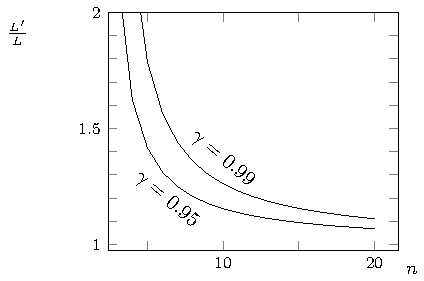
\includegraphics{knownUnknownVarianceConfidenceIntervalRatioGamma}
\caption{
\عددی{\gamma=0.95} اور \عددی{\gamma=0.99} لیتے ہوئے وقفہ اعتماد کی لمبائی \عددی{L'} (مساوات \حوالہ{مساوات_شماریات_وقفہ_اعتماد_ب}) اور \عددی{L} (مساوات \حوالہ{مساوات_شماریات_وقفہ_اعتماد_الف}) کی نسبت بالمقابل نمونی جسامت \عددی{n}، جہاں \عددی{s} اور \عددی{\sigma} ایک جیسے ہیں۔ 
}
\label{شکل_مثال_شماریات_ٹی_تقسیم_وقفہ_اعتماد}
\end{figure}
\انتہا{مثال}
%===========================
جدول \حوالہ{جدول_شماریات_وقفہ_اعتماد_پ} میں عمومی تقسیم کی تغیریت کا وقفہ اعتماد تعین کرنے کے قدم دیے گئے ہیں۔ جو جدول \حوالہ{جدول_شماریات_وقفہ_اعتماد_الف} اور جدول \حوالہ{جدول_شماریات_وقفہ_اعتماد_ب} کی طرح ہیں، پس، یہاں دو مستقل \عددی{c_1} اور \عددی{c_2} حاصل کرنے ہوں گے۔دونوں مستقل  کو ضمیمہ \حوالہ{ضمیمہ_جدول} میں جدول \حوالہ{ضمیمہ_مربع_خا_تقسیم} سے حاصل کیا جاتا ہے جس میں تفاعل تقسیم
\begin{align}\label{مساوات_شماریات_مربع_خا}
F(z)=
\begin{cases}
C_m\int_0^z e^{^{-u}\!/\!_2}\,u^{^{(m-2)}\!/\!_2}\dif u& z\ge 0\\[1ex]
0&z<0
\end{cases}
\end{align}
کی قیمتوں کے لئے \عددی{z} کے مطابقتی قیمتیں دی گئی ہیں۔اس تقسیم کو \عددی{\chi^2}تقسیم (مربع خا تقسیم)\شناخت{صفحہ_شماریات_مربع_خا_تقسیم} کہتے ہیں۔یہاں
 \عددی{C_m=\tfrac{1}{[2^{m\!/\!_2}\Gamma(^m\!/\!_2)]}} اور \عددی{m=1,2,\cdots} مقدار معلوم ہے جس کو تقسیم کی درجہ آزادی کی تعداد کہتے ہیں۔

%============================
\begin{table}
\caption{عمومی تقسیم کی تغیریت $\sigma^2$ کے وقفہ اعتماد کا تعین جہاں اوسط جاننا ضروری نہیں ہے}
\label{جدول_شماریات_وقفہ_اعتماد_پ}
\centering
\fbox{
\begin{minipage}{0.95\textwidth}
\موٹا{پہلا قدم:}\quad
وقفہ اعتماد منتخب کریں مثلاً \عددی{\gamma=\SI{95}{\percent}} یا \عددی{\gamma=\SI{99}{\percent}}، وغیرہ۔\\
\موٹا{دوسرا قدم:}\quad 
درج ذیل مساوات کے حل \عددی{c_1} اور \عددی{c_2}
\begin{align}\label{مساوات_شماریات_عمومی_تقسیم_خا_شرائط}
F(c_1)=\frac{1}{2}(1-\gamma),\quad F(c_2)=\frac{1}{2}(1+\gamma)
\end{align}
کو   مربع خا تقسیم کی جدول (ضمیمہ \حوالہ{ضمیمہ_جدول}، جدول \حوالہ{ضمیمہ_مربع_خا_تقسیم}، جسامت نمونہ=\عددی{n}) سے \عددی{n-1} درجہ آزادی کے لئے حاصل کریں۔ 
\موٹا{تیسرا قدم:}\quad 
نمونہ \عددی{x_1,\cdots,x_n} کی تغیریت \عددی{s^2} سے \عددی{(n-1)s^2} حاصل کریں۔\\
\موٹا{چوتھا قدم:} \quad 
\عددی{k_1=\tfrac{(n-1)s^2}{c_1}} اور \عددی{k_2=\tfrac{(n-1)s^2}{c_2}} کا حساب لگائیں۔ وقفہ اعتماد درج ذیل ہو گا۔
\begin{align}\label{مساوات_شماریات_وقفہ_اعتماد_پ}
\text{اعتماد}\{k_2\le \sigma^{\,2} \le k_1\}
\end{align}
\end{minipage}
}
\end{table}
%================================
\ابتدا{مثال}\quad \موٹا{عمومی تقسیم کے تغیریت کا وقفہ اعتماد}\\
جدول \حوالہ{جدول_شماریات_تعددی_تقسیم_الف} میں دیا گیا نمونہ استعمال کرتے ہوئے مطابقتی آبادی کے تغیریت کا وقفہ اعتماد تلاش کریں۔\\
حل:\quad
\موٹا{پہلا قدم:}\quad
\عددی{\gamma=0.95} درکار ہے۔\\
\موٹا{دوسرا قدم:}\quad
چونکہ \عددی{n=100} ہے لہٰذا ہم \عددی{c_1=73.4} اور \عددی{c_2=128} حاصل کرتے ہیں۔\\
\موٹا{تیسرا قدم:}\quad
جدول \حوالہ{جدول_شماریات_تعددی_تقسیم_الف} سے \عددی{99s^2=71291} حاصل ہوتا ہے۔\\
\موٹا{چوتھا قدم:}\quad
وقفہ اعتماد درج ذیل ہو گا۔
\begin{align*}
\text{اعتماد}\{ 556\le \sigma^{\,2} \le 972\}
\end{align*}
\انتہا{مثال}
%====================================

\جزوحصہء{دیگر تقسیمات}
کافی بڑے نمونے لیتے ہوئے دیگر تقسیمات کی اوسط اور تغیریت کے وقفہ اعتماد گزشتہ تراکیب سے حاصل کیے جا سکتے ہیں۔عملاً، اگر نا معلوم تقسیم کا ترچھاپن کم ہو تب \عددی{\mu} کا وقفہ اعتماد حاصل کرنے کے لئے  نمونی جسامت کم سے کم \عددی{n=20} لینی چاہیے  اور \عددی{\sigma^2} کا وقفہ اعتماد کے لئے کم سے کم \عددی{n=50} لینا چاہیے۔ اس  کی تفصیل اس حصے کے آخر میں پیش کی جائے گی۔

\جزوحصہء{جدول \حوالہ{جدول_شماریات_وقفہ_اعتماد_الف}، جدول \حوالہ{جدول_شماریات_وقفہ_اعتماد_ب} اور جدول \حوالہ{جدول_شماریات_وقفہ_اعتماد_پ} میں دیے گئے تراکیب کا نظریہ}
ہم اب درج ذیل سادہ تصور استعمال کرتے ہوئے اس نظریہ پر غور کرتے ہیں جو وقفہ اعتماد حاصل کرنے کی ان تراکیب کو ممکن بناتی ہے۔

اب تک ہم نمونی قیمتوں \عددی{x_1,\cdots,x_n} کو واحد بلا منصوبہ متغیر \عددی{X} کی  مشاہدے سے حاصل \عددی{n} قیمتیں تصور کرتے رہے ہیں۔ہم ان \عددی{n} قیمتوں کو \عددی{n} بلا منصوبہ متغیرات \عددی{X_1,\cdots,X_n}، جن کی تقسیم ایک جیسی ہے (جو \عددی{X} کی تقسیم ہے)، کی  ایک مشاہدے کی قیمتیں بھی تصور کر سکتے ہیں جنہیں غیر تابع اس لئے تصور کیا جا سکتا ہے کہ نمونی قیمتیں کو غیر تابع تصور کیا گیا ہے۔

 جدول \حوالہ{جدول_شماریات_وقفہ_اعتماد_الف} میں مساوات \حوالہ{مساوات_شماریات_وقفہ_اعتماد_الف} اخذ کرنے  کے لئے درج ذیل درکار ہو گا۔

%=====================
\ابتدا{مسئلہ}\شناخت{مسئلہ_شماریات_بلا_منصوبہ_عمومی_متغیرات_مجموعہ}\quad \موٹا{(بلا منصوبہ عمومی متغیرات کا مجموعہ)}\\
فرض کریں کہ \عددی{X_1,X_2,\cdots,X_n} بلا منصوبہ غیر تابع عمومی متغیرات ہیں جن کے اوسط بالترتیب \عددی{\mu_1,\cdots,\mu_n} اور تغیریت بالترتیب \عددی{\sigma^{\,2}_1,\cdots,\sigma^{\,2}_n} ہیں۔ تب بلا منصوبہ متغیر
\begin{align*}
X=X_1+X_2+\cdots+X_n
\end{align*}
عمومی ہو گا جس کی اوسط
\begin{align*}
\mu=\mu_1+\mu_2+\cdots+\mu_n
\end{align*}
اور تغیریت
\begin{align*}
\sigma^{\,2}=\sigma^{\,2}_1+\sigma^{\,2}_2+\cdots+\sigma^{\,2}_n
\end{align*}
ہو گی۔\عددی{\mu} اور \عددی{\sigma^2} کے فقرے مسئلہ \حوالہ{مسئلہ_شماریات_مجموعہ_اوسط} اور مسئلہ \حوالہ{مسئلہ_شماریات_تغیرات_کا_مجموعہ} دیتے ہیں جبکہ \عددی{X} عمومی ہونے کا ثبوت اس کتاب میں پیش نہیں کیا جائے گا۔
\انتہا{مسئلہ}
%========================

اس مسئلے سے اور مسئلہ \حوالہ{مسئلہ_شماریات_خطی_تبادل_دوسرا} اور مسئلہ \حوالہ{مسئلہ_شماریات_معیاری_متغیر} سے درج ذیل حاصل ہوتا ہے۔

%=============
\ابتدا{مسئلہ}\شناخت{مسئلہ_شماریات_عمومی_کی_شرط_اوسط_تغیریت}\quad
اگر \عددی{X_1,\cdots, X_n} غیر تابع عمومی بلا منصوبہ متغیرات ہوں جن میں سے ہر ایک کی اوسط \عددی{\mu} اور تغیریت \عددی{\sigma^2} ہو، تب بلا منصوبہ متغیر
\begin{align}\label{مساوات-شماریات_غیر_تابع_متغیرات_اوسط_تغیریت_الف}
\overline{X}=\frac{1}{n}(X_1+\cdots+X_n)
\end{align}
عمومی ہو گا جس کی اوسط \عددی{\mu} اور تغیریت \عددی{\tfrac{\sigma^2}{n}} ہو گی، اور بلا منصوبہ متغیر
\begin{align}\label{مساوات-شماریات_غیر_تابع_متغیرات_اوسط_تغیریت_ب}
Z=\sqrt{n}\,\frac{\overline{X}-\mu}{\sigma}
\end{align}
عمومی ہو گا جس کی اوسط \عددی{0} اور تغیریت \عددی{1} ہو گی۔
\انتہا{مسئلہ}
%=======================

آئیں مساوات \حوالہ{مساوات_شماریات_وقفہ_اعتماد_الف} اخذ کرتے ہیں۔اس حصے کی شروع میں ہم نے چاہا کہ ہم ایسے دو بلا منصوبہ متغیرات \عددی{\Theta_1} اور \عددی{\Theta_2} حاصل کریں جو درج ذیل کو مطمئن کرتے ہوں
\begin{align}\label{مساوات-شماریات_غیر_تابع_متغیرات_اوسط_تغیریت_پ}
P(\Theta_1\le \mu\le \Theta_2)=\gamma
\end{align}
جہاں \عددی{\gamma} منتخب کردہ ہے، اور نمونہ سے مشاہدے کے ذریعہ \عددی{\Theta_1} کی قیمت \عددی{\theta_1} اور \عددی{\Theta_2} کی قیمت \عددی{\theta_2} حاصل کرتے ہوئے درج ذیل  وقفہ اعتماد  حاصل کیا جاتا ہے۔
\begin{align*}
\text{اعتماد}\{\theta_1\le \mu\le\theta_2\}
\end{align*}
موجودہ صورت میں ایسا کرنے کی خاطر ہم \عددی{\gamma} کی قیمت \عددی{0} اور \عددی{1} کے بیچ منتخب کرتے ہیں اور  ضمیمہ \حوالہ{ضمیمہ_جدول} کی جدول \حوالہ{ضمیمہ_عمومی_تقسیم_ب} سے ایسا \عددی{c} حاصل کرتے ہیں جو \عددی{P(-c\le Z\le z)=\gamma} کو مطمئن کرتا ہو۔ (جدول \حوالہ{جدول_شماریات_وقفہ_اعتماد_الف} میں \عددی{\gamma} کی مختلف قیمتوں کے لئے \عددی{c} کی قیمتیں اسی طرح حاصل کی گئی ہیں۔) مساوات \حوالہ{مساوات-شماریات_غیر_تابع_متغیرات_اوسط_تغیریت_الف} میں دیا گیا \عددی{Z} استعمال کرتے ہوئے عدم مساوات \عددی{-c\le Z\le c} درج ذیل صورت اختیار کرتی ہے
\begin{align*}
-c\le \sqrt{n}\,\frac{\overline{X}-\mu}{\sigma}\le c
\end{align*}
جس کو \عددی{\mu} کی عدم مساوات میں تبدیل کیا جا سکتا ہے۔اس کو \عددی{\tfrac{\sigma}{\sqrt{n}}} سے ضرب کر  \عددی{k=\tfrac{c\sigma}{\sqrt{n}}} لکھتے ہوئے  \عددی{-k\le \overline{X}-\mu\le k} ملتا ہے۔اس کو \عددی{-1} سے ضرب دے کر \عددی{\overline{X}} جمع کرتے ہوئے درج ذیل حاصل ہو گا۔
\begin{align}\label{مساوات-شماریات_غیر_تابع_متغیرات_اوسط_تغیریت_ت}
\overline{X}+k\ge \mu\ge \overline{X}-k
\end{align}
یوں \عددی{P(-c\le Z\le c)=\gamma} سے مراد \عددی{P(\overline{X}-k\le \mu\le \overline{X}+k)=\gamma} ہے جو 
 مساوات \حوالہ{مساوات-شماریات_غیر_تابع_متغیرات_اوسط_تغیریت_پ} کی طرز کا ہے جہاں \عددی{\Theta_1=\overline{X}-k} اور \عددی{\Theta_2=\overline{X}+k} ہوں گے۔یوں ہمارے مفروضوں کے تحت بلا منصوبہ متغیرات \عددی{\overline{X}-k} اور \عددی{\overline{X}+k} وہ قیمتیں اختیار کریں گے جن میں نا معلوم اوسط \عددی{\mu} شامل ہو گا۔ جہاں تک \عددی{n} غیر تابع عمومی بلا منصوبہ متغیرات \عددی{X_1,\cdots,X_n} کی مشاہدہ سے حاصل، جدول \حوالہ{جدول_شماریات_وقفہ_اعتماد_الف} میں دی گئی،  نمونی قیمتیں \عددی{x_1,\cdots,x_n}  ہیں، ہم دیکھتے ہیں کہ نمونی اوسط \عددی{\overline{x}} مساوات \حوالہ{مساوات-شماریات_غیر_تابع_متغیرات_اوسط_تغیریت_الف} کی مشاہدہ سے حاصل قیمت ہے جس کو مساوات \حوالہ{مساوات-شماریات_غیر_تابع_متغیرات_اوسط_تغیریت_ت} میں پر کرتے ہوئے مساوات \حوالہ{مساوات_شماریات_وقفہ_اعتماد_الف} حاصل ہوتا ہے۔


مساوات \حوالہ{مساوات_شماریات_وقفہ_اعتماد_ب} اخذ کرنے کی خاطر ہمیں درج ذیل درکار ہو گا۔
%==================
\ابتدا{مسئلہ}\شناخت{مسئلہ_شماریات_ٹی_تقسیم_اوسط_تغیریت}\quad
فرض کریں کہ \عددی{X_1,\cdots,X_n} غیر تابع عمومی بلا منصوبہ متغیرات ہیں جن میں ہر ایک کی اوسط \عددی{\mu} اور تغیریت \عددی{\sigma^{\,2}} ہے۔تب بلا منصوبہ متغیر
\begin{align}
T=\sqrt{n}\,\frac{\overline{X}-\mu}{S}
\end{align}
کی تقسیم \عددی{n-1} درجہ آزادی کی \عددی{t} تقسیم (صفحہ \حوالہصفحہ{صفحہ_شماریات_ٹی_تقسیم}) ہو گی؛ یہاں \عددی{\overline{X}} کو مساوات 
\حوالہ{مساوات-شماریات_غیر_تابع_متغیرات_اوسط_تغیریت_الف} اور
\begin{align}\label{مساوات_شماریات_مسئلہ_مربع_ایس}
S^2=\frac{1}{n-1}\sum_{j=1}^{n} \big(X_j-\overline{X}\big)^2
\end{align}
دیتے ہیں۔ اس مسئلے کا ثبوت اس کتاب میں پیش نہیں کیا جائے گا۔
\انتہا{مسئلہ}
%======================

مساوات \حوالہ{مساوات_شماریات_وقفہ_اعتماد_ب} کا ثبوت مساوات \حوالہ{مساوات_شماریات_وقفہ_اعتماد_الف} کی ثبوت کی طرح کا ہے۔ہم \عددی{\gamma} کی قیمت \عددی{0} اور \عددی{1} کے بیچ  منتخب کرتے ہوئے  ضمیمہ \حوالہ{ضمیمہ_جدول} کی جدول \حوالہ{ضمیمہ_ٹی_تقسیم} سے \عددی{n-1} درجہ آزادی کا  ایسا \عددی{c} حاصل کرتے ہیں جو درج ذیل کو مطمئن کرتا ہو۔
\begin{align}\label{مساوات_شماریات_ٹی_تقسیم_ثبوت_الف}
P(-c\le T\le c)=F(c)-F(-c)=\gamma
\end{align}
چونکہ \عددی{t} تقسیم تشاکلی ہے لہٰذا \عددی{F(-c)=1-F(c)} ہو گا اور یوں مساوات \حوالہ{مساوات_شماریات_ٹی_تقسیم_ثبوت_الف}  سے مساوات \حوالہ{مساوات_شماریات_ٹی_تقسیم_وقفہ_اعتماد} حاصل ہو گا۔مساوات \حوالہ{مساوات_شماریات_ٹی_تقسیم_ثبوت_الف} میں پہلے کی طرح \عددی{-c\le T\le c} کے تبادلہ سے
\begin{align}\label{مساوات_شماریات_ٹی_تقسیم_ثبوت_ب}
\overline{X}-K\le \mu\le \overline{X}+K\quad\quad K=\frac{cS}{\sqrt{n}}
\end{align}
حاصل ہو گا اور یوں مساوات \حوالہ{مساوات_شماریات_ٹی_تقسیم_ثبوت_الف} سے \عددی{P(\overline{X}-K\le \mu\le \overline{X}+K)=\gamma} حاصل ہو گا۔مساوات \حوالہ{مساوات_شماریات_ٹی_تقسیم_ثبوت_ب} میں مشاہدے سے  حاصل \عددی{\overline{X}} کی قیمت \عددی{\overline{x}} اور \عددی{S^2} کی قیمت \عددی{s^2} پر کرتے ہوئے مساوات \حوالہ{مساوات_شماریات_وقفہ_اعتماد_ب} حاصل ہو گا۔

مساوات \حوالہ{مساوات_شماریات_وقفہ_اعتماد_پ} ثابت کرنے کی خاطر ہمیں درج ذیل کی ضرورت ہو گی۔

%=====================
\ابتدا{مسئلہ}\شناخت{مسئلہ_شماریات_مربع_خا_تقسیم_کا_درجہ_آزادی}\quad
مسئلہ \حوالہ{مسئلہ_شماریات_ٹی_تقسیم_اوسط_تغیریت} کے مفروضوں کے تحت بلا منصوبہ متغیر
\begin{align}\label{مساوات_شماریات_مسئلہ_وائے}
Y=(n-1)\,\frac{S^2}{\sigma^{\,2}}
\end{align}
کا تقسیم  \عددی{n-1} درجہ آزادی کا مربع خا تقسیم (صفحہ \حوالہصفحہ{صفحہ_شماریات_مربع_خا_تقسیم}) ہو گا؛ یہاں \عددی{S^2} کو مساوات \حوالہ{مساوات_شماریات_مسئلہ_مربع_ایس} میں پیش کیا گیا ہے۔

اس مسئلے کا ثبوت اس کتاب میں پیش نہیں کیا جائے گا۔
\انتہا{مسئلہ}
%========================

مساوات \حوالہ{مساوات_شماریات_وقفہ_اعتماد_پ} کا ثبوت مساوات \حوالہ{مساوات_شماریات_وقفہ_اعتماد_الف} اور مساوات \حوالہ{مساوات_شماریات_وقفہ_اعتماد_ب} کی ثبوتوں کی طرح ہے۔ہم \عددی{0} اور \عددی{1} کے بیچ عدد \عددی{\gamma} منتخب کرتے ہیں۔ضمیمہ \حوالہ{ضمیمہ_جدول} میں جدول \عددی{ضمیمہ_مربع_خا_تقسیم} سے ایسے  \عددی{c_1} اور \عددی{c_2} کی حاصل کریں جو درج ذیل (مساوات \حوالہ{مساوات_شماریات_عمومی_تقسیم_خا_شرائط}) کو مطمئن کرتے ہوں۔
\begin{align*}
P(Y\le c_1)=F(c_1)=\frac{1}{2}(1-\gamma),\quad P(Y\le c_2)=F(c_2)=\frac{1}{2}(1+\gamma)
\end{align*}
تفریق سے
\begin{align*}
P(c_1\le Y\le c_2)=P(Y\le c_2)-P(Y\le c_1)=\gamma
\end{align*}
حاصل ہوتا ہے۔مساوات \حوالہ{مساوات_شماریات_مسئلہ_وائے} میں دیے \عددی{Y} سے \عددی{c_1\le Y\le c_2} کے تبادلہ سے \عددی{\sigma^{\,2}} کی عدم مساوات حاصل کرتے ہوئے ہم 
\begin{align*}
\frac{n-1}{c_2}S^2\le \sigma^{\,2} \le \frac{n-1}{c_1}S^2
\end{align*} 
حاصل کرتے ہیں۔مشاہدے سے حاصل \عددی{S^2} کی قیمت \عددی{s^2} کرتے ہوئے  مساوات \حوالہ{مساوات_شماریات_وقفہ_اعتماد_پ} حاصل ہو گا۔

%=================
\جزوحصہء{دیگر تقسیمات کی اوسط اور تغیریت کے وقفہ اعتماد}
دیگر تقسیمات کے لئے بھی ہم وقفہ اعتماد کو جدول \حوالہ{جدول_شماریات_وقفہ_اعتماد_الف}، جدول \حوالہ{جدول_شماریات_وقفہ_اعتماد_ب} اور جدول \حوالہ{جدول_شماریات_وقفہ_اعتماد_پ} سے حاصل کر سکتے ہیں، پس نمونوں کی جسامت بڑی رکھنی ہو گی۔یہ درج ذیل مسئلہ کہتا ہے۔

%=====================
\ابتدا{مسئلہ}\شناخت{مسئلہ_شماریات_متقاربی_عمومی}\quad \موٹا{(مسئلہ وسطی حد)}\\
فرض کریں کہ \عددی{X_1,\cdots,X_m,\cdots} غیر تابع بلا منصوبہ متغیرات ہیں جن کی تقسیم ایک جیسی ہے لہٰذا ان کی اوسط \عددی{\mu} ایک جیسی ہو گی اور ان کی تغیریت \عددی{\sigma^{\,2}}  ایک جیسی ہو گی۔فرض کریں کہ \عددی{Y_n=X_1+\cdots+X_n} ہے تب بلا منصوبہ متغیر
\begin{align}
Z_n=\frac{Y_n-n\mu}{\sigma \sqrt{n}}
\end{align}
\اصطلاح{متقاربی عمومی}\فرہنگ{متقاربی عمومی}\فرہنگ{عمومی!متقاربی}\حاشیہب{asymptotically normal}\فرہنگ{normal!asymptotically} ہو گا جس کی اوسط \عددی{0} اور تغیریت \عددی{1} ہو گی، یعنی، \عددی{Z_n} کا تفاعل تقسیم \عددی{F_n(x)} درج ذیل کو مطمئن کرے گا
\begin{align*}
\lim_{n\to \infty} F_n(x)=\Phi(x)=\frac{1}{\sqrt{2\pi}}\int_{-\infty}^{\infty} e^{-\tfrac{u^2}{2}}\dif u
\end{align*}
جس کا ثبوت اس کتاب میں پیش نہیں کیا جائے گا۔
\انتہا{مسئلہ}
%===========================

ہم جانتے ہیں کہ اگر \عددی{X_1,\cdots,X_n} غیر تابع بلا منصوبہ متغیرات ہوں جن کی ایک جیسی اوسط \عددی{\mu} اور ایک جیسی تغیریت \عددی{\sigma^{\,2}} ہو، تب ان کے مجموعہ \عددی{X=X_1+\cdots+X_n} کے درج ذیل خواص ہوں گے۔
\begin{itemize}
\item{(الف)}
\عددی{X} کی اوسط \عددی{n\mu} اور تغیریت \عددی{n\sigma^{\,2}} ہو گی (مسئلہ \حوالہ{مسئلہ_شماریات_مجموعہ_اوسط} اور  مسئلہ \حوالہ{مسئلہ_شماریات_تغیرات_کا_مجموعہ})۔
\item{(ب)}
اگر یہ متغیرات عمومی ہوں تب \عددی{X} بھی عمومی ہو گا (مسئلہ \حوالہ{مسئلہ_شماریات_بلا_منصوبہ_عمومی_متغیرات_مجموعہ})۔
\end{itemize}

اگر یہ متغیرات عمومی نہ ہوں تب مذکورہ بالا  شق-ب درست نہیں ہو گا، البتہ بڑی \عددی{n} کی صورت میں \عددی{X} تخمیناً عمومی  (مسئلہ \حوالہ{مسئلہ_شماریات_متقاربی_عمومی}) ہو گا اور یہی وجہ ہے کہ \عددی{n} کی قیمت بڑی لیتے ہوئے  ان تراکیب  کو دیگر تقسیمات کے لئے بھی  استعمال کیا جا سکتا ہے۔

%=====================
\حصہء{سوالات}
%===================
\ابتدا{سوال}\quad
عمومی صورتوں میں نقطی اندازہ سے وقفی اندازہ کیوں زیادہ کار آمد ہوتے ہیں؟   
\انتہا{سوال}
%========================
\ابتدا{سوال}\شناخت{سوال_شماریات_نمونہ_دیا_الف}\quad
\عددی{100} جسامت کا نمونہ جس کی اوسط \عددی{38.25} ہو استعمال کرتے ہوئے  عمومی آبادی جس کی تغیریت \عددی{\sigma^{\,2}=9} ہے کی اوسط \عددی{\mu} کے لئے \عددی{\SI{95}{\percent}} وقفہ اعتماد تعین کریں۔
\انتہا{سوال}
%========================
\ابتدا{سوال}\quad
نمونی جسامت کو گھٹا کر \عددی{25} کرنے سے سوال \حوالہ{سوال_شماریات_نمونہ_دیا_الف} میں وقفہ اعتماد  پر کیا اثر ہو گا؟\\
جواب:\quad
وقفہ اعتماد دگنا ہو جائے گا۔
\انتہا{سوال}
%===========================
\ابتدا{سوال}\quad
نمونہ \عددی{28,24,31,27,22} استعمال کرتے ہوئے معیاری انحراف \عددی{\sigma=2.2} والی عمومی آبادی کی اوسط کے لئے \عددی{\SI{99}{\percent}} وقفی اعتماد تعین کریں۔ 
\انتہا{سوال}
%========================
\ابتدا{سوال}\quad
اوسط \عددی{16.30} اور جسامت \عددی{290}  والا نمونہ استعمال کرتے ہوئے  شکل \حوالہ{شکل_شماریات_وقفہ_لمبائی_بالمقابل_جسامت} کی مدد سے تغیریت \عددی{\sigma^2=0.36} والی عمومی آبادی کی اوسط کے لئے \عددی{\SI{99}{\percent}} وقفی اعتماد تعین کریں۔\\
جواب:\quad
$\text{اعتماد} \{16.21\le \mu\le 16.39\}$
\انتہا{سوال}
%=========================
\ابتدا{سوال}\quad
مساوات \حوالہ{مساوات_شماریات_وقفہ_اعتماد_الف} میں \عددی{\SI{95}{\percent}} وقفہ اعتماد کی لمبائی (الف) \عددی{2\sigma} (ب) \عددی{\sigma} حاصل کرنے  کے لئے درکار نمونی جسامت \عددی{n} تلاش کریں۔
\انتہا{سوال}
%======================

سوال \حوالہ{سوال_شماریات_عمومی_آبادی_درکار_اوسط_الف} تا سوال \حوالہ{سوال_شماریات_عمومی_آبادی_درکار_اوسط_ب} میں فرض کریں کہ دیا گیا نمونہ  عمومی آبادی سے حاصل کیا گیا ہے۔آبادی کی اوسط \عددی{\mu} کے لئے \عددی{\SI{99}{\percent}} وقفہ اعتماد تعین کریں۔

%================
\ابتدا{سوال}\شناخت{سوال_شماریات_عمومی_آبادی_درکار_اوسط_الف} \quad
$325,320,325,335$\\
جواب:\quad
$\text{اعتماد} \{307\le \mu\le 345\}$
\انتہا{سوال}
%========================
\ابتدا{سوال}\quad
\عددی{20} قابلوں کا نمونہ جس کی اوسط \عددی{\SI{10.20}{\centi\meter}} اور تغیریت \عددی{\sigma^2=\SI{0.04}{\centi\meter\squared}} ہو۔
\انتہا{سوال}
%==========================
\ابتدا{سوال}\quad
سلاخ کی ملی میٹروں میں لمبائی
$124, 127,126,122,124$\\
جواب:\quad
$\text{اعتماد} \{120.6\le \mu\le 128.6\}$
\انتہا{سوال}
%========================
\ابتدا{سوال}\quad
پشاور تا لاہور موٹروے پر بلا منصوبہ \عددی{500} گاڑیوں کو روک کر ان کے بریک پرکھے جاتے ہیں جن میں سے \عددی{87} گاڑیوں کے بریک کمزور ثابت ہوتے ہیں۔اس نمونہ کو استعمال کرتے ہوئے موٹروے پر کمزور بریک والی گاڑیوں کی فی صد  کے لئے \عددی{\SI{95}{\percent}} وقفہ اعتماد تعین کریں۔
\انتہا{سوال}
%======================
\ابتدا{سوال}\شناخت{سوال_شماریات_عمومی_آبادی_درکار_اوسط_ب}\quad
ثنائی تقسیم کی مقدار معلوم \عددی{p} کے لئے \عددی{\SI{99}{\percent}} وقفہ اعتماد تعین کریں۔صفحہ \حوالہصفحہ{جدول_شماریات_سکہ_پھینکنے_کے_نتائج} پر جدول \حوالہ{جدول_شماریات_سکہ_پھینکنے_کے_نتائج} کی آخری صف میں  مشرف کے نتائج استعمال کریں۔\\
جواب:\quad
$\text{اعتماد}  \{ 0.492\le p \le 0.509\}$
\انتہا{سوال}
%========================

سوال \حوالہ{سوال_شماریات_عمومی_آبادی_وقفہ_الف} تا سوال \حوالہ{سوال_شماریات_عمومی_آبادی_وقفہ_الف} میں عمومی آبادی سے نمونے حاصل کیے گیے ہیں۔آبادی کی تغیریت \عددی{\sigma^2} کی \عددی{\SI{95}{\percent}} وقفہ اعتماد تعین کریں۔

%==================
\ابتدا{سوال}\شناخت{سوال_شماریات_عمومی_آبادی_وقفہ_الف}\quad
$145.3, 145.1, 145.4,146.2$
\انتہا{سوال}
%=======================
\ابتدا{سوال}\quad
نمونی جسامت \عددی{30} اور تغیریت \عددی{0.0007} ہے۔\\
جواب:\quad
$\text{اعتماد} \{0.00044\le \sigma^2\le 0.00127\}$
\انتہا{سوال}
%=======================
\ابتدا{سوال}\quad
درجہ حرارت کمرہ پر ایک مخصوص قسم کی دھات کی مطلق تنشی مضبوطی (\عددی{\si{\kilo\gram\per\centi\meter\squared}}):
$17.6,19.7,18.1,17.8,17.8,17.7,17.6,17.7,17.9,18$
\انتہا{سوال}
%========================
\ابتدا{سوال}\quad
یورینیم \عددی{\ce{U^{35}}} کی انشقاق سے پیدا تاخیری نیوٹران  گروہ (تیسرا گروہ جس کی نصف زندگی \عددی{6.2} سیکنڈ ہے) کی اوسط توانائی (\si{\kilo\electronvolt}):
$435,451,430,444,438$\\
جواب:\quad
$\text{اعتماد} \{23\le\sigma^2\le553\}$
\انتہا{سوال}
%==========================
\ابتدا{سوال}\quad
\عددی{\SI{80}{\kilo\meter\per\hour}} کی رفتار سے سفر کرتے ہوئے ایک گاڑی کی فی کلومیٹر خارج کردہ
 \عددی{\ce{CO}} (گرام): $10.8,11.1,11.2,11,11.3,10.8,10.9,11.2$  
\انتہا{سوال}
%==========================
\ابتدا{سوال}\quad
اگر \عددی{X} عمومی ہو جس کی اوسط \عددی{27} اور تغیریت \عددی{16} ہو تب \عددی{-X}، \عددی{3X} اور \عددی{5X-2} کے تقسیم، اوسط اور تغیریت کیا ہوں گے؟\\
جواب:\quad
تینوں عمومی، اوسط \عددی{-27,81,133} اور تغیریت \عددی{16,144,400} ہوں گے۔
\انتہا{سوال}
%=======================
\ابتدا{سوال}\quad
اگر \عددی{X_1} اور \عددی{X_2} غیر تابع عمومی بلا منصوبہ متغیرات ہوں جن کی اوسط بالترتیب \عددی{23}، \عددی{4} اور تغیریت  بالترتیب \عددی{3}، \عددی{1}  ہوں تب \عددی{4X_1-X_2} کی تقسیم، اوسط اور تغیریت کیا ہوں گے؟
\انتہا{سوال}
%===========================
\ابتدا{سوال}\quad
ایک مشین \عددی{Y} کلوگرام کمیت کے ڈبوں میں \عددی{X} کلوگرام نمک بھرتی ہے جہاں \عددی{X} اور \عددی{Y} کی اوسط بالترتیب \عددی{100} کلوگرام، \عددی{5} کلوگرام اور تغیریت بالترتیب \عددی{1} کلوگرام، \عددی{0.5} کلوگرام ہیں۔کتنے فی صد بھرے گیے  ڈبوں کی کمیت \عددی{104} کلوگرام اور \عددی{106} کلوگرام کے بیچ ہو گی؟\\
جواب:\quad
$P(104\le Z\le 106)=\SI{63}{\percent}$
\انتہا{سوال}
%======================
\ابتدا{سوال}\quad
اگر سیمنٹ کی بوری کی کمیت \عددی{X} عمومی متغیر ہو جس کی اوسط \عددی{\SI{40}{\kilo\gram}} اور تغیریت \عددی{\SI{2}{\kilo\gram}} ہو تب ایک ٹرک میں کتنی بوریاں رکھی جا سکتی ہیں تا کہ بوریوں کی  کل کمیت کا \عددی{\SI{2000}{\kilo\gram}} سے تجاوز کرنے کا احتمال \عددی{\SI{5}{\percent}} ہو۔
\انتہا{سوال}
%=========================

\حصہ{قیاس کی پرکھ۔ فیصلے}\شناخت{حصہ_شماریات_قیاس_کی_پرکھ_فیصلے}
بلا منصوبہ متغیر کی تقسیم کے بارے میں کچھ فرض کرنے کو شماریاتی \اصطلاح{قیاس}\فرہنگ{قیاس}\حاشیہب{hypothesis}\فرہنگ{hypothesis} کہتے ہیں۔مثال کے طور پر کسی تقسیم کے بارے میں یہ فرض کرنا کہ اس کی اوسط \عددی{20.3} ہے شماریات قیاس ہو گا۔ایسا عمل  جس سے ہم معلوم کر سکیں کہ آیا ہمارا قیاس  ٹھیک ہے اور ہم اس کو \اصطلاح{منظور}\فرہنگ{منظور}\حاشیہب{accept, not reject}\فرہنگ{reject!not} کریں یا کہ یہ غلط ہے اور ہم اس کو \اصطلاح{نا منظور}\فرہنگ{منظور!نا}\حاشیہب{reject}\فرہنگ{reject} کریں شماریاتی \اصطلاح{پرکھ}\فرہنگ{پرکھ}\حاشیہب{test}\فرہنگ{test} کہلاتا ہے۔

یہ پرکھ عموماً استعمال کیے جاتے ہیں اور ہم جاننا چاہیں گے کہ یہ کیوں اہم ہیں۔ہمیں عموماً ایسی صورتوں میں فیصلہ کرنا ہوتا ہے جہاں امکانی تبدیلیاں عمل پیرا ہوتی ہیں۔مثال کے طور پر اگر ہمیں دو ممکنات میں سے ایک کو چننا ہو، ہمارا فیصلہ کسی شماریاتی پرکھ پر منحصر ہو سکتا ہے۔

مثال کے طور پر اگر ہمیں ایک خراد کی مشین پر قابلے بنانا ہو جن کی قطر مخصوص حدود میں رہنا ضروری ہو اور ہم چاہتے ہیں کہ زیادہ سے زیادہ \عددی{\SI{2}{\percent}} قابلے عیب دار ہوں تب ہم اس خراد پر بنائے گئے قابلوں سے \عددی{100} قابلوں کا نمونہ حاصل کرتے ہوئے قیاس \عددی{\sigma^2=\sigma^2_0} کو پرکھ کر دیکھیں گے کہ آیا مطابقتی آبادی کی تغیریت \عددی{\sigma^2} کسی مخصوص قیمت \عددی{\sigma^2_0} کے برابر ہے۔\عددی{\sigma^2_0} کو یوں منتخب کیا جاتا ہے کہ زیادہ سے زیادہ  \عددی{\SI{2}{\percent}} قابلے عیب دار حاصل ہوں۔اس کا \ترچھا{متبادل}\فرہنگ{پرکھ!متبادل} پرکھ \عددی{\sigma^2>\sigma^2_0} ہے۔ہم پرکھ کے نتیجہ کو دیکھ کر قیاس \عددی{\sigma^2=\sigma^2_0} کو \ترچھا{منظور} کرتے ہوئے اسی خراد کو استعمال کرتے ہیں یا ہم اس کو \ترچھا{نا منظور} کرتے ہوئے کہتے ہیں کہ \عددی{\sigma^2>\sigma^2_0} ہے اور اس سے بہتر خراد استعمال کرتے ہیں۔نا منظوری کی صورت میں ہم کہتے ہیں کہ \عددی{\sigma^2_0} سے \عددی{\sigma^2} کا \اصطلاح{معنی خیز انحراف}\فرہنگ{انحراف!معنی خیز}\حاشیہب{significant deviation}\فرہنگ{deviation!significant} پایا جاتا ہے، یعنی انحراف نا گزیر  امکانی وجوہات کی بنا نہیں ہے بلکہ خراد کی ناقص پن کی وجہ سے ہے۔

ہو سکتا ہے کہ کسی دوسری جگہ پر ہمیں دو چیزوں کا آپس میں موازنہ کرنا ہو، مثلاً، دو ادویات، ایک کام سرانجام دینے کے دو تراکیب، ناپنے کے دو طریقے، دو مشینوں پر بنائے گئے چیزوں کی معیار، وغیرہ وغیرہ۔ موزوں پرکھ کے نتیجہ کے تحت ہم ایک دوائی کو منتخب کریں گے، کام کرنے کی بہتر ترکیب منتخب کریں گے، وغیرہ۔

قیاس عمومی درج ذیل سے حاصل ہو گا۔
\begin{itemize}
\item
ضرورت معیاری پیداوار سے قیاس پیش کیا جا سکتا ہے۔(سخت نگرانی اور احتیاط کے ساتھ زیادہ تعداد کی چیزیں پیدا کرنے سے قابل حصول معیار کے بارے میں تجربہ حاصل ہوتا ہے۔)\\
\item
گزشتہ تجربہ سے حاصل معلوم قیمتوں پر قیاس منحصر ہو سکتا ہے۔\\
\item
قیاس ایک نظریہ پر مبنی ہو سکتا ہے جس کو آپ پرکھنا چاہتے ہیں۔\\
\item
بعض اوقات اتفاقی مشاہدے پر قیاس مبنی ہو سکتا ہے۔   
\end{itemize}  

آئیں ایک تعارفی مثال سے شروع کرتے ہیں۔

%===================
\ابتدا{مثال}\شناخت{مثال_شماریات_لڑکا_یا_لڑکی}\quad \موٹا{قیاس کا پرکھ}\\
ایک بچہ پیدا ہونے کو بلا منصوبہ تجربہ تصور کیا جا سکتا ہے جس کے دو ممکنہ انجام ہیں، یعنی لڑکا \عددی{B} اور لڑکی \عددی{G}۔ وجدانی طور پر ہم قیاس کر  سکتے ہیں کہ دونوں کا احتمال ایک جیسا ہو گا البتہ کچھ لوگوں کا \ترچھا{متبادل} قیاس ہے کہ  نو زائدہ بچوں میں لڑکوں کی تعداد زیادہ ہوتی ہے۔ہم قیاس کو پرکھنا چاہتے ہیں۔اگر ہم انجام \عددی{B} کے احتمال کو \عددی{p} سے ظاہر کریں تب ہم قیاس \عددی{p=\SI{50}{\percent}=0.5} کو پرکھا جا سکتا ہے۔متبادل قیاس \عددی{p>0.5} کو بھی پرکھا جا سکتا ہے۔ہم ایسا ہی کرتے ہیں۔

اس پرکھ کے لئے ایک شہر میں ایک سال میں پیدا بچوں  سے  ہم \عددی{n=3000} نمونہ منتخب کرتے ہیں جن میں سے \عددی{1578} لڑکے ہیں۔

اگر قیاس درست ہو تب  \عددی{n=3000} کی نمونہ میں اوسطاً تقریباً \عددی{1500} نو زائدہ لڑکے متوقع ہوں گے۔اگر متبادل درست ہو تب \عددی{1500} سے اوسطاً زائد لڑکے متوقع ہوں گے۔یوں اگر حقیقتاً نو زائدہ لڑکوں کی تعداد \عددی{1500} سے بہت زیادہ ہو تب ہم اس کو  قیاس غلط ہونے کی نشانی تصور کرتے ہوئے  قیاس  کو نا منظور کریں گے۔

ہم سب سے پہلے ایک فاصل قیمت \عددی{c} متعین کرتے ہیں۔ متبادل کی بنا \عددی{c} کی قیمت \عددی{1500} سے زیادہ ہو گی۔(\عددی{c} تعین کرنے کا ایک طریقہ نیچے پیش کیا گیا ہے۔) تب نو زائد لڑکوں کی تعداد \عددی{c} سے زیادہ ہونے کی صورت میں ہم قیاس کو نا منظور کریں گے اور اگر نو زائد لڑکوں کی تعداد  \عددی{c} سے زیادہ نہ ہو تب ہم قیاس کو منظور کریں گے۔

اب ہمیں \عددی{c} کی ایسی قیمت  منتخب کرنی ہو گی جو معمولی بلا منصوبہ انحراف اور زیادہ معنی خیز انحراف میں تمیز کرے۔ہر شخص کی اپنی ایک منفرد رائے ہو سکتی ہے لیکن ہمیں حسابی دلائل  کے تحت چلنا ہو گا جو موجودہ صورت میں بہت سادہ ہیں (جیسے آپ اب دیکھیں گے)۔

ہم \عددی{c} یوں تعین کرتے ہیں کہ قیاس درست ہونے کی صورت میں \عددی{c} سے زیادہ لڑکوں کا احتمال بہت کم ہو مثلاً \عددی{\alpha}۔ روایتی طور پر \عددی{\alpha=\SI{1}{\percent}} یا \عددی{\alpha=\SI{5}{\percent}} منتخب کیا جاتا ہے۔ \عددی{\alpha=\SI{1}{\percent}} (یا \عددی{\alpha=\SI{5}{\percent}}) منتخب کرتے ہوئے ہم \عددی{100} میں (یا \عددی{20} میں) \عددی{1} زیادہ لڑکوں کی صورت میں بھی قیاس کو نا منظور کرتے ہیں اگرچہ قیاس درست ہے۔اس نقطے پر ہم بعد میں غور کریں گے۔آئیں ہم \عددی{\alpha=\SI{1}{\percent}} منتخب کرتے ہوئے درج ذیل بلا منصوبہ متغیر پر غور کرتے ہیں۔
\begin{align*}
X=\text{\RL{پیدائشوں میں لڑکوں کی تعداد}} \,3000\,\text{\RL{بچوں کی}}
\end{align*}
یہ فرض کرتے ہوئے قیاس درست ہے ہم \عددی{c} کی فاصل قیمت کو درج ذیل کلیہ سے حاصل کرتے ہیں
\begin{align}\label{مساوات_شماریات_قیاس_فاصل_قیمت_الف}
P(X>c)_{p=0.5}=\alpha=0.01
\end{align}
جہاں مفروضے کو زیر نوشت میں \عددی{p=0.5} سے ظاہر کیا گیا ہے۔اگر لڑکوں کی حقیقی تعداد \عددی{1578} منتخب \عددی{c} سے زیادہ ہو تب ہم قیاس کو نا منظور کریں گے۔اگر \عددی{1578\le c} ہو تب ہم قیاس کو منظور کریں گے۔

 مساوات \حوالہ{مساوات_شماریات_قیاس_فاصل_قیمت_الف} سے \عددی{c} حاصل کرنے کی خاطر ہمیں \عددی{X} کی تقسیم  معلوم ہونی چاہیے۔موجودہ مثال کے لئے ثنائی تقسیم کافی درست ہے۔یوں اگر قیاس درست ہو تب ثنائی تقسیم میں \عددی{X} کی \عددی{p=0.5} اور \عددی{n=300} ہوں گے۔اس تقسیم کو تخمینی طور پر ایسی عمومی تقسیم سے  ظاہر کیا جا سکتا ہے جس کی اوسط \عددی{\mu=np} اور تغیریت \عددی{\sigma^2=npq=750} ہو (حصہ \حوالہ{حصہ_شماریات_عمومی_تقسیم})۔ (ہم اپنی آسانی کی خاطر مساوات \حوالہ{مساوات_شماریات_ڈی_موے_ب} میں جزو \عددی{0.5} کو رد کرتے ہیں۔) تقسیم کی منحنی کو شکل \حوالہ{شکل_مثال_شماریات_لڑکا_یا_لڑکی} میں دکھایا گیا ہے۔ مساوات \حوالہ{مساوات_شماریات_قیاس_فاصل_قیمت_الف} استعمال کرتے ہوئے درج ذیل حاصل ہوتا ہے۔
\begin{align*}
P(X>c)=1-P(X\le c)\approx 1-\Theta\big(\frac{c-1500}{\sqrt{750}}\big)=0.01
\end{align*}
ضمیمہ \حوالہ{ضمیمہ_جدول} کی جدول \حوالہ{ضمیمہ_عمومی_تقسیم_ب} سے \عددی{\tfrac{c-1500}{\sqrt{750}}=2.326} حاصل ہوتا ہے  لہٰذا \عددی{c=1564} ہو گا۔چونکہ \عددی{1578>c} ہے لہٰذا ہم قیاس کو نا منظور کرتے ہوئے فیصلہ کرتے ہیں کہ \عددی{p>0.5} ہے۔یوں پرکھ مکمل ہوتا ہے۔

\عددی{300} کے نمونہ کے لئے  مساوات \حوالہ{مساوات_شماریات_قیاس_فاصل_قیمت_الف} میں \عددی{X} کو \عددی{300} پیدائشوں میں لڑکوں کی تعداد لیتے ہوئے  فاصل قیمت \عددی{c=170} حاصل ہو گی اور نمونہ میں \عددی{158} (جو وہی فی صد ہے جو  بڑی جسامت کے نمونہ میں تھی)  لڑکے ہونے کی صورت میں \عددی{158<c} حاصل ہو گا اور ہم قیاس کو منظور کریں گے۔یہ ایک دلچسپ صورت حال ہے جس سے یہ حقیقت اجاگر ہوتی ہے کہ پرکھ کی افادیت نمونی جسامت \عددی{n} بڑھانے سے بڑھتی ہے۔ہمیں \عددی{n} اتنا بڑا لینا ہو گا کہ عملی صورت میں زیر غور متغیر کے بارے میں درست نتائج حاصل ہوں۔ساتھ ہی ساتھ \عددی{n} زیادہ بڑا بھی نہیں ہونا چاہیے تا کہ وقت اور سرمایہ کا ضیاع نہ ہو۔عموماً صورتوں میں پہلے چھوٹا تجربہ کرتے ہوئے بہتر \عددی{n} کو تعین کرنا ممکن ہو گا۔  
\begin{figure}
\centering
\begin{tikzpicture}
\begin{axis}[small,axis lines*=middle,axis y line=none,xtick={1450,1500,1550,1600},xticklabels={$1450$,$1500$,$1550$,$1600$},ytick={0}, yticklabels={$0$}]
\addplot[domain=1450:1600,smooth]{1/(sqrt(750)*sqrt(2*pi))*e^(-0.5*((x-1500)^2/750))}node[pos=0.80,pin=50:{$\SI{1}{\percent}$}]{};
\addplot[black,dashed]  coordinates {(1564,-0.002) (1564,0.016)}node[pos=0,below,font=\small]{$c=1564$};
\addplot[] coordinates {(1564,-0.004)};
\addplot[] coordinates {(1540,0.014)}node[]{\RL{قیاس منظور}};
\addplot[] coordinates {(1590,0.014)}node[]{\RL{قیاس نا منظور}};
\addplot[] coordinates {(1500,0.004)}node[font=\small]{$\SI{99}{\percent}$};
\end{axis}
\end{tikzpicture}
\caption{درست قیاس کی صورت میں $X$ کی تخمینی تقسیم ( مثال \حوالہ{مثال_شماریات_لڑکا_یا_لڑکی})۔فاصل قیمت $c=1564$ ہے}
\label{شکل_مثال_شماریات_لڑکا_یا_لڑکی}
\end{figure}
\انتہا{مثال}
%=========================

\جزوحصہء{متبادل کا تصور۔متبادل کی قسمیں}
جس قیاس کو پرکھا جا رہا ہو اس کو \اصطلاح{پسندیدہ قیاس}\فرہنگ{قیاس!پسندیدہ}\حاشیہب{default hypothesis}\فرہنگ{hypothesis!default} کہتے ہیں اور اس کا مخالفانہ  قیاس (مثلاً مثال \حوالہ{مثال_شماریات_لڑکا_یا_لڑکی} میں \عددی{p>0.5}) کو \ترچھا{متبادل قیاس}\فرہنگ{قیاس!متبادل}\حاشیہب{alternative hypothesis}\فرہنگ{hypothesis!alternative} یا مختصراً \ترچھا{متبادل} کہتے ہیں۔ عدد \عددی{\alpha} (یا \عددی{100\alpha\si{\percent}}) کو پرکھ کی  \اصطلاح{معنی خیز سطح}\فرہنگ{معنی خیز سطح}\حاشیہب{significant level}\فرہنگ{significant!level} کہتے ہیں جبکہ \عددی{c} \اصطلاح{فاصل قیمت}\فرہنگ{فاصل!قیمت}\حاشیہب{critical value}\فرہنگ{critical!value} کہلاتا ہے۔ جس خطے میں وہ قیمتیں پائی جاتی ہوں جن کے لئے قیاس کو نا منظور کیا جاتا ہے، اس خطے کو \اصطلاح{خطہ نا منظوری}\فرہنگ{خطہ!نا منظوری}\فرہنگ{نا منظوری!خطہ}\حاشیہب{rejection region}\فرہنگ{region!rejection} یا \اصطلاح{خطہ فاصل}\فرہنگ{خطہ!فاصل}\حاشیہب{critical region}\فرہنگ{region!critical}  کہتے ہیں۔وہ خطہ جس میں پائے جانے والی قیمتوں کے لئے قیاس کو منظور کیا جاتا ہے \اصطلاح{خطہ منظوری}\فرہنگ{خطہ!منظوری}\حاشیہب{acceptance region}\فرہنگ{region!acceptance} کہلاتا ہے۔\عددی{\alpha} کو عموماً \عددی{\alpha=\SI{5}{\percent}} منتخب کیا جاتا ہے۔

فرض کریں کہ ایک تقسیم میں مقدار معلوم \عددی{\theta} کی قیمت نا معلوم ہے۔فرض کریں کہ ہم قیاس \عددی{\theta=\theta_0} کو پرکھنا چاہتے ہیں۔اس کے درج ذیل تین متبادل قیاس پائے جاتے ہیں۔
\begin{align}
\theta &>\theta_0 \label{مساوات_شماریات_متبادل_پرکھ_الف}\\
\theta&<\theta_0 \label{مساوات_شماریات_متبادل_پرکھ_ب}\\
\theta&\ne \theta_0 \label{مساوات_شماریات_متبادل_پرکھ_پ}
\end{align}
مساوات \حوالہ{مساوات_شماریات_متبادل_پرکھ_الف}  اور مساوات \حوالہ{مساوات_شماریات_متبادل_پرکھ_ب}  کو \اصطلاح{یک طرفہ متبادل}\فرہنگ{متبادل!یک طرفہ}\حاشیہب{one-sided alternatives}\فرہنگ{alternative!one-sided} جبکہ مساوات \حوالہ{مساوات_شماریات_متبادل_پرکھ_پ}  کو \اصطلاح{دو طرفہ متبادل}\فرہنگ{متبادل!دو طرفہ}\حاشیہب{two-sided alternative}\فرہنگ{alternative!two-sided} کہتے ہیں۔مثال \حوالہ{مثال_شماریات_لڑکا_یا_لڑکی} میں دو طرفہ متبادل پر غور کیا گیا (جہاں \عددی{\theta_0=p=0.5} اور \عددی{\theta_0=p>0.5} تھے)؛ \عددی{\theta_0} کی دائیں جانب \عددی{c} پایا جاتا ہے اور خطہ نا منظور \عددی{c} سے لے کر \عددی{\infty} ہو گا اور اس پرکھ کو \اصطلاح{دایاں طرفہ پرکھ}\فرہنگ{پرکھ!دایاں طرفہ}\حاشیہب{right-sided test}\فرہنگ{test!right-sided} کہتے ہیں۔مساوات \حوالہ{مساوات_شماریات_متبادل_پرکھ_ب} میں \عددی{\theta_0} کی بائیں جانب \عددی{c} پایا جاتا ہے، اور خطہ نا منظوری \عددی{c} سے \عددی{-\infty} تک ہو گا
 (شکل \حوالہ{شکل_شماریات_خطہ_منظور_اور_نا_منظوری}) اور اس پرکھ کو \اصطلاح{بایاں طرفہ پرکھ}\فرہنگ{پرکھ!بایاں طرفہ}\فرہنگ{alternative!left-sided} کہیں گے۔ان دونوں قسم کے پرکھ کو \ترچھا{یک طرفہ پرکھ} کہتے ہیں۔مساوات \حوالہ{مساوات_شماریات_متبادل_پرکھ_پ} کی صورت میں ہمارے پاس دو فاصل قیمتیں \عددی{c_1} اور \عددی{c_2\, (>c_1)} ہوں گی اور خطہ نا منظوری \عددی{c_1} تا \عددی{-\infty} اور \عددی{c_2} تا \عددی{\infty} ہو گا، اور پرکھ کو \اصطلاح{دو طرفہ پرکھ}\فرہنگ{پرکھ!دو طرفہ}\فرہنگ{test!two-sided} کہیں گے۔

\begin{figure}
\centering
\begin{tikzpicture}
\shade[gray,shading angle=180](5,0) rectangle (8,0.2);
\draw(0,0)--++(8,0);
\draw(4,0)node[below]{$\theta_0$}--++(0,0.2);
\draw[thick](5,0)node[below]{$c$}--++(0,1);
\draw(2,0.8)node[align=right,font=\small]{\RL{خطہ منظوری} \\ \RL{قیاس نا منظور نہ کریں}\\ \RL{(قیاس منظور کریں)}};
\draw(6.5,0.8)node[align=right,font=\small]{\RL{خطہ نا منظوری}\\  \RL{(خطہ فاصل)}\\  \RL{قیاس نا منظور کریں}};
%
\begin{scope}[yshift=-2cm]
\shade[gray,shading angle=180](0,0) rectangle (3,0.2);
\draw(0,0)--++(8,0);
\draw(4,0)node[below]{$\theta_0$}--++(0,0.2);
\draw[thick](3,0)node[below]{$c$}--++(0,1);
\draw(1.5,0.8)node[align=right,font=\small]{\RL{خطہ نا منظوری}\\  \RL{(خطہ فاصل)}\\  \RL{قیاس نا منظور کریں}};
\draw(6,0.8)node[align=right,font=\small]{\RL{خطہ منظوری} \\ \RL{قیاس نا منظور نہ کریں}\\ \RL{(قیاس منظور کریں)}};
\end{scope}
%
\begin{scope}[yshift=-4cm]
\shade[gray,shading angle=180](5,0) rectangle (8,0.2);
\shade[gray,shading angle=180](0,0) rectangle (3,0.2);
\draw(0,0)--++(8,0);
\draw(4,0)node[below]{$\theta_0$}--++(0,0.2);
\draw[thick](3,0)node[below]{$c_1$}--++(0,1);
\draw[thick](5,0)node[below]{$c_2$}--++(0,1);
\draw(1.5,0.8)node[align=right,font=\small]{\RL{خطہ نا منظوری}\\  \RL{(خطہ فاصل)}\\  \RL{قیاس نا منظور کریں}};
\draw(4,0.8)node[align=right,font=\small]{\RL{خطہ منظوری} \\ \RL{قیاس نا منظور نہ کریں}\\ \RL{(قیاس منظور کریں)}};
\draw(6.5,0.8)node[align=right,font=\small]{\RL{خطہ نا منظوری}\\  \RL{(خطہ فاصل)}\\  \RL{قیاس نا منظور کریں}};
\end{scope}
\end{tikzpicture}
\caption{مساوات \حوالہ{مساوات_شماریات_متبادل_پرکھ_الف} کی متبادل (بالائی شکل)، مساوات \حوالہ{مساوات_شماریات_متبادل_پرکھ_ب} کی متبادل (درمیانی شکل) اور مساوات \حوالہ{مساوات_شماریات_متبادل_پرکھ_پ} کی متبادل (نچلی شکل) کی صورت میں پرکھ}
\label{شکل_شماریات_خطہ_منظور_اور_نا_منظوری}
\end{figure}

تینوں اقسام کے متبادل عملاً اہم ہیں۔ مثال کے طور پر مساوات \حوالہ{مساوات_شماریات_متبادل_پرکھ_ب} مادہ کی  مضبوطی کی پرکھ میں ہمیں پیش آ سکتا ہے جہاں \عددی{\theta_0} درکار مضبوطی ہو سکتی ہے جبکہ متبادل غیر پسندیدہ کمزوری کو ظاہر کرے گا۔درکار قیمت سے زیادہ مضبوطی کی صورت میں مادہ منظور کیا جائے گا لہٰذا اس کو علیحدہ سے پرکھنے کی ضرورت نہیں ہو گی۔ مساوات \حوالہ{مساوات_شماریات_متبادل_پرکھ_پ} ایسی صورت میں اہم ہو گا جیسے دھرا کی قطر جہاں \عددی{\theta_0} درکار قطر کو ظاہر کرے گا جبکہ اس سے کم یا زیادہ موٹائی دونوں برابر مسئلہ خیز ہوں گے  لہٰذا درکار موٹائی کے دونوں جانب انحراف پر نظر رکھنا ضروری ہو گا۔

\جزوحصہء{پرکھ میں غلطیوں کے اقسام} 
ہم اب متبادل، جس کو ہم اپنی آسانی کی خاطر واحد عدد \عددی{\theta_1} تصور کرتے ہیں،  کے لحاظ سے قیاس \عددی{\theta=\theta_0} کے پرکھ سے غلط فاصلوں کے خطرات پر غور کرتے ہیں۔ فرض کریں \عددی{\theta_1>\theta_0} ہے لہٰذا ہمارے پاس دایاں طرفہ پرکھ ہو گا۔ (بایاں طرفہ یا دو طرفہ پرکھ  کے لئے بھی صورت حال ایسا ہی ہو گا۔) دیے گیے نمونہ \عددی{x_1,\cdots,x_n} سے ہم  قیمت \عددی{\widehat{\theta}=g(x_1,\cdots,x_n)}  کا حساب لگاتے ہیں۔اگر \عددی{\widehat{\theta}>c} ہو تب قیاس کو نا منظور کیا جاتا ہے (جیسا مثال \حوالہ{مثال_شماریات_لڑکا_یا_لڑکی} میں کیا گیا)۔ اگر \عددی{\widehat{\theta}\le c} ہو تب قیاس کو منظور کیا جاتا ہے۔ 
\عددی{\widehat{\theta}} کی قیمت کو بلا منصوبہ متغیر
\begin{align*}
\widehat{\Theta}=g(X_1,\cdots,X_n)
\end{align*}
کی مشاہدے سے حاصل قیمت تصور کیا جا سکتا ہے چونکہ \عددی{x_j} کو \عددی{X_j} کی مشاہدے سے حاصل قیمت تصور کیا جا سکتا ہے، جہاں \عددی{j=1,\cdots,n} ہے۔ان پرکھ میں غلطی کرنے کے درج ذیل  دو امکانات  پائے جاتے ہیں۔

\جزوحصہء{غلطی قسم اول}
جدول \حوالہ{جدول_شماریات_پرکھ_درست_لیکن_نا_منظور} میں پرکھ درست ہے لیکن \عددی{\Theta} قیمت \عددی{\widehat{\theta}>c} اختیار کرتا ہے جس کی بنا  اس پرکھ کو نا منظور کیا جاتا ہے (لہٰذا متبادل کو منظور کیا جاتا ہے) ظاہر ہے کہ ایسی غلطی کا احتمال
\begin{align}\label{مساوات_شماریات_غلطی_احتمال_الف}
P(\widehat{\Theta}>c)_{\theta=\theta_0}=\alpha
\end{align}
ہو گا جو معنی خیز سطح کے برابر ہے۔

\begin{table}
\caption{متبادل $\theta=\theta_1$ کے لحاظ سے قیاس $\theta=\theta_0$ کی پرکھ میں پہلی اور دوسری قسم کا خلل}
\label{جدول_شماریات_پرکھ_درست_لیکن_نا_منظور}
\centering
\begin{otherlanguage}{english}
\begin{tabular}{cc|cc}
\hline
&&\multicolumn{2}{c}{\RL{\urdufont{نا معلوم حقیقت}}}\Tstrut\\
&&$\theta=\theta_0$&$\theta=\theta_1$\\
\hline 
\parbox[t]{2mm}{\multirow{4}{*}{\rotatebox[origin=c]{90}{\urdufont{منظور}}}}&\multirow{2}{*}{ $\theta=\theta_0$}&\RL{\urdufont{ٹھیک فیصلہ}} & \multicolumn{1}{|c}{\RL{\urdufont{دوسری قسم کا خلل}}}\Tstrut\\
&& $P=1-\alpha$&\multicolumn{1}{|c}{ $P=\beta$}\\
\cline{2-4}
&\multirow{2}{*}{$\theta=\theta_1$}& \RL{\urdufont{پہلی قسم کا خلل}} &\multicolumn{1}{|c}{\RL{\urdufont{ٹھیک فیصلہ}}}\\
&&$P=\alpha$& \multicolumn{1}{|c}{$P=a-\beta$}\\
\hline
\end{tabular}
\end{otherlanguage}
\end{table}

\جزوحصہء{غلطی قسم دوم}
جدول \حوالہ{جدول_شماریات_پرکھ_درست_لیکن_نا_منظور} پر نظر رکھیں۔قیاس غلط ہے لیکن اس کو منظور کیا جاتا ہے، چونکہ \عددی{\widehat{\Theta}} قیمت \عددی{\widehat{\theta}\le c} اختیار کرتا ہے۔ایسی غلطی کرنے کے احتمال کو \عددی{\beta} سے ظاہر کیا جاتا ہے؛ لہٰذا
\begin{align}\label{مساوات_شماریات_غلطی_احتمال_ب}
P(\widehat{\Theta}\le c)_{\theta=\theta_1}=\beta
\end{align}
ہو گا۔  \عددی{\eta=1-\beta} کو پرکھ کی \اصطلاح{طاقت}\فرہنگ{پرکھ!طاقت}\حاشیہب{power}\فرہنگ{test!power} کہتے ہیں جو غلطی کی قسم دوم سے بچنے کا احتمال ہے۔

مساوات \حوالہ{مساوات_شماریات_غلطی_احتمال_الف} اور مساوات \حوالہ{مساوات_شماریات_غلطی_احتمال_ب} سے ظاہر ہے کہ \عددی{\alpha} اور \عددی{\beta} دونوں \عددی{c} پر منحصر ہیں اور ہم چاہیں گے کہ ہم ایسا \عددی{c} منتخب کریں کہ غلطیاں کرنے کے احتمال کم سے کم ہوں۔البتہ شکل \حوالہ{شکل_شماریات_غلطیاں} سے ظاہر ہوتا ہے کہ یہ متصادم ضروریات ہیں۔\عددی{\alpha} گھٹانے کی خاطر \عددی{c} کو دائیں منتقل کرنا ہو گا جس سے \عددی{\beta} بڑھتا ہے۔ حقیقت میں ہم \عددی{\alpha} (\عددی{\SI{5}{\percent}} یا \عددی{\SI{1}{\percent}}) منتخب کر کے \عددی{c} تعین کرتے ہیں اور آخر میں \عددی{\beta} کا حساب کرتے ہیں۔ اگر \عددی{\beta} بڑی ہو جس سے  طاقت \عددی{\eta=1-\beta} چھوٹی حاصل ہو گی تب ہمیں زیادہ بڑا نمونہ (جس کی وجہ جلد سامنے آئے گی) لے کر پرکھ دہرانا چاہیے۔ 
\begin{figure}
\centering
\begin{tikzpicture}
\begin{axis}[clip=false,small,axis lines*=middle, axis y line=none,xtick={2,4,6},xticklabels={$\theta_0$,$c$,$\theta_1$}]
\pgfmathsetmacro{\nab}{1.2}
\addplot[domain=0:6,smooth] {e^(-1/2*((x-2)/\nab)^2)}node[pos=0.35,above left,align=right]{\RL{$\widehat{\Theta}$ کی کثافت} \\ \RL{اگر قیاس درست ہو}};
\addplot[dashed,domain=1:8,smooth] {e^(-1/2*((x-5)/\nab)^2)}node[pos=0.55,above right,align=right]{\RL{$\widehat{\Theta}$ کی کثافت}\\  \RL{اگر متبادل درست ہو}};
\addplot[black] coordinates {(4,0) (4,1)};
\addplot[mark=none] coordinates {(3,0.075)}node[]{$\beta$};
\addplot[] coordinates {(4.5,0.05)}node[]{$\alpha$};
\addplot[] coordinates {(4,-0.2) (4,-0.3)};
\addplot[stealth-]coordinates {(4,-0.25) (3,-0.25)}node[left]{\RL{خطہ منظوری}};
\addplot[stealth-]coordinates {(4,-0.25) (5,-0.25)}node[right]{\RL{خطہ نا منظوری (خطہ فاصل)}};
\end{axis} 
\end{tikzpicture}
\caption{قیاس $\theta=\theta_0$ بالمقابل متبادل $\theta=\theta_1\,(>\theta_0)$ کی پرکھ میں قسم اول اور دوم غلطیوں کی وضاحت}
\label{شکل_شماریات_غلطیاں}
\end{figure}

اگر متبادل واحد عدد نہ ہو بلکہ مساوات \حوالہ{مساوات_شماریات_متبادل_پرکھ_الف} تا مساوات \حوالہ{مساوات_شماریات_متبادل_پرکھ_پ} کی طرح ہو  تب \عددی{\beta} تفاعل ہو گا جو  \عددی{\theta} کا تابع ہو گا۔تفاعل \عددی{\beta(\theta)} کو پرکھ کی \اصطلاح{خاصیت کارکردگی}\فرہنگ{کارکردگی!خاصیت}\حاشیہب{operating characteristic}\فرہنگ{characteristic!operating} کہتے ہیں اور اس کی منحنی کو \اصطلاح{منحنی خاصیت کارکردگی}\فرہنگ{خاصیت!منحنی کارکردگی} کہتے ہیں۔ظاہر ہے کہ ایسی صورت میں \عددی{\eta=1-\beta} بھی \عددی{\theta} کے تابع ہو گا اور تفاعل \عددی{\eta(\theta)} کو پرکھ کا \اصطلاح{تفاعل طاقت}\فرہنگ{طاقت!تفاعل}\حاشیہب{power function}\فرہنگ{power!function} کہتے ہیں۔

ظاہر ہے کہ ایسی پرکھ جس کی بنا کوئی قیاس \عددی{\theta_0} منظور ہو سے یہ ظاہر نہیں ہوتا کہ یہی سب سے بہتر  یا واحد قیاس ہے۔یوں لفظ "منظور" کی جگہ "نا منظور نہ کرنا" کہنا زیادہ بہتر ہو گا۔ 

 \جزوحصہء{عمومی تقسیم کی صورت میں پرکھ}
درج ذیل مثال عملاً اہم قیاس کے پرکھ کی وضاحت کرتا ہے۔ 

%==============
\ابتدا{مثال}\شناخت{مثال_شماریات_معلوم_تغیریت_عمومی_تقسیم_کی_اوسط}\quad \موٹا{(معلوم تغیریت کی عمومی تقسیم کی اوسط کا پرکھ)}\\
فرض کریں کہ \عددی{X} بلا منصوبہ متغیر ہے جس کی تغیریت \عددی{\sigma^2=9} ہے۔نمونی جسامت \عددی{n=10} لیتے ہوئے قیاس \عددی{\mu=\mu_0=24} کو درج ذیل تین متبادل کے بالمقابل پرکھیں۔
\begin{align*}
\text{(پ)}\,\,\, \mu \ne \mu_0 \quad \text{(ب)}\,\,\, \mu<\mu_0 \quad \text{(الف)}\,\,\,  \mu>\mu_0
\end{align*}
حل:\quad
ہم معنی خیز سطح \عددی{\alpha=0.05} منتخب کرتے ہیں۔اوسط کی اندازاً قیمت درج ذیل سے حاصل ہو گی۔
\begin{align*}
\overline{X}=\frac{1}{n}(X_1+\cdots,X_n)
\end{align*}
اگر قیاس درست ہو تب \عددی{X} عمومی ہو گا جس کی اوسط \عددی{\mu=24} اور تغیریت \عددی{\tfrac{\sigma^2}{n}=0.9} ہو گی (مسئلہ \حوالہ{مسئلہ_شماریات_عمومی_کی_شرط_اوسط_تغیریت})۔لہٰذا ہم فاصل قیمت \عددی{c} کو ضمیمہ \حوالہ{ضمیمہ_جدول} کی جدول \حوالہ{ضمیمہ_عمومی_تقسیم_ب} سے حاصل کر سکتے ہیں۔\\
\موٹا{صورت الف:}\quad
ہم \عددی{P(\overline{X}\le c)_{\mu=24}=\alpha=0.05} سے \عددی{c} تعین کرتے ہیں۔
\begin{align*}
P(\overline{X}\le c)_{\mu=24}=\Phi\big(\frac{c-24}{\sqrt{0.9}}\big)=1-\alpha=0.95
\end{align*}
ضمیمہ \حوالہ{ضمیمہ_جدول} کی جدول \حوالہ{ضمیمہ_عمومی_تقسیم_ب}  سے \عددی{\tfrac{c-24}{\sqrt{0.9}}=1.645} یعنی \عددی{c=25.56} حاصل ہوتا ہے جو \عددی{\mu_0} سے بڑی قیمت ہے (اور جو شکل \حوالہ{شکل_شماریات_خطہ_منظور_اور_نا_منظوری} میں سب سے اوپر دکھائی گئی صورت ہے)۔ اگر \عددی{\overline{x}\le 25.56} ہو تب قیاس کو منظور کیا جائے گا۔ اگر \عددی{\overline{x}>25.56} ہو تب قیاس کو نا منظور کیا جائے گا۔پرکھ کی طاقت درج ذیل ہو گی (شکل \حوالہ{شکل_مثال_شماریات_معلوم_تغیریت_عمومی_تقسیم_کی_اوسط} الف)۔
\begin{gather}
\begin{aligned}
\eta(\mu)=P(\overline{X}>25.56)_{\mu}&=1-P(\overline{X}\le 25.56)_{\mu}\\
&=1-\Phi\big(\frac{25.56-\mu}{\sqrt{0.9}}\big)=1-\Phi(26.94-1.05\mu)
\end{aligned}
\end{gather}
%=================
\begin{figure}
\centering
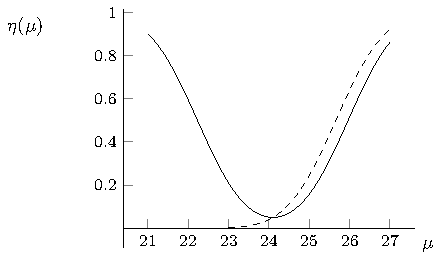
\includegraphics{normalWithKnownVariance}
\caption{طاقت $\eta(\mu)$؛ مثال \حوالہ{مثال_شماریات_معلوم_تغیریت_عمومی_تقسیم_کی_اوسط}  الف (نقطہ دار خط) اور پ (ٹھوس خط)}
\label{شکل_مثال_شماریات_معلوم_تغیریت_عمومی_تقسیم_کی_اوسط}
\end{figure}
\موٹا{صورت ب:}\quad
فاصل قیمت \عددی{c} کو درج ذیل مساوات سے حاصل کیا جا سکتا ہے۔
\begin{align*}
P(\overline{X}\le c)_{\mu=24}=\Phi\big(\frac{c-24}{\sqrt{0.9}}\big)=\alpha=0.05
\end{align*}
ضمیمہ \حوالہ{ضمیمہ_جدول} کی جدول \حوالہ{ضمیمہ_عمومی_تقسیم_ب}  سے \عددی{c=24-1.56=22.24} ملتا ہے۔اگر \عددی{\overline{x}\ge 22.44} ہو تب ہم قیاس کو منظور کرتے ہیں۔اگر \عددی{\overline{x}<22.44} ہو تب ہم قیاس کو نا منظور کرتے ہیں۔پرکھ کی طاقت درج ذیل ہے۔
\begin{align}
\eta(\mu)=P(\overline{X}\le 22.44)_{\mu}=\Phi\big(\frac{22.44-\mu}{\sqrt{0.9}}\big)=\Phi(23.65-1.05\mu)
\end{align}
\موٹا{صورت پ:}\quad
چونکہ عمومی تقسیم تشاکلی ہے، ہم \عددی{\mu=24} سے \عددی{c_1} اور \عددی{c_2} کو ایک جیسے فاصلے پر چن کر، مثلاً \عددی{c_1=24-k} اور \عددی{c_2=24+k}، مستقل \عددی{k} کو درج ذیل سے تعین کرتے ہیں۔
\begin{align*}
P(24-k\le \overline{X}\le 24+k)_{\mu=24}=\Phi\big(\frac{k}{\sqrt{0.9}}\big)-\Phi\big(-\frac{k}{\sqrt{0.9}}\big)=1-\alpha=0.95
\end{align*}
ضمیمہ \حوالہ{ضمیمہ_جدول} کی جدول \حوالہ{ضمیمہ_عمومی_تقسیم_ب} سے \عددی{\tfrac{k}{\sqrt{0.9}}=1.960} یعنی \عددی{k=1.86} حاصل ہو گا۔یوں \عددی{c_1=24-1.86=22.14} اور \عددی{c_2=24+1.86=25.86} ہوں گے۔اگر \عددی{\overline{x}} کی قیمت \عددی{c_1} سے چھوٹی نہ ہو اور \عددی{c_2} سے بڑی نہ ہو تب ہم قیاس کو منظور کرتے ہیں۔اس کے علاوہ ہم قیاس کو نا منظور کرتے ہیں۔پرکھ کی طاقت درج ذیل ہے (شکل \حوالہ{شکل_مثال_شماریات_معلوم_تغیریت_عمومی_تقسیم_کی_اوسط} پ)۔
\begin{gather}
\begin{aligned}
\eta(\mu)&=P(\overline{X}<22.14)_{\mu}+P(\overline{X}>25.86)_{\mu}\\
&=P(\overline{X}<22.14)_{\mu}+1-P(\overline{X}\le 25.86)_{\mu}\\
&=1+\Phi\big(\frac{22.14-\mu}{\sqrt{0.9}}\big)-\Phi\big(\frac{25.86-\mu}{\sqrt{0.9}}\big)\\
&=1+\Phi(23.34-1.05\mu)-\Phi(27.26-1.05\mu)
\end{aligned}
\end{gather}
نتیجتاً خاصیت کارکردگی \عددی{\beta(\mu)=1-\eta(\mu)} درج ذیل ہو گی۔
\begin{align*}
\beta(\mu)&=\Phi\big(\frac{24.59-\mu}{\sqrt{0.9}}\big)-\Phi\big(\frac{23.41-\mu}{\sqrt{0.9}}\big)\\
&=\Phi(81.97-3.33\mu)-\Phi(78.03-3.33\mu)
\end{align*}
شکل \حوالہ{شکل_مثال_شماریات_معلوم_تغیریت_عمومی_تقسیم_کی_اوسط_کارکردگی} سے ظاہر ہے کہ \عددی{n=10} کی خاصیت کارکردگی کی مطابقتی منحنی کی ڈھلوان زیادہ ہے۔اس کا مطلب ہے کہ \عددی{n} بڑھانے سے بہتر پرکھ حاصل ہوتا ہے۔کسی بھی عملی استعمال میں \عددی{n} کو کم سے کم لیکن اتنا زیادہ رکھا جاتا ہے کہ پرکھ \عددی{\mu} اور \عددی{\mu_0} میں انحراف، جس میں ہم دلچسپی رکھتے ہیں، کو  واضح  کرے۔ مثال کے طور پر اگر انحراف ہماری دلچسپی  \عددی{\mp 2} اکائی ہو، ہم شکل سے دیکھتے ہیں کہ \عددی{n=10} بہت کم ہو گا چونکہ جب \عددی{\mu=24-2=22} یا \عددی{\mu=24+2=26} ہو تب \عددی{\beta} تقریباً \عددی{\SI{50}{\percent}} ہو گا۔اس کے برعکس ، \عددی{n=100} اس صورت کافی ہو گا۔
\begin{figure}
\centering
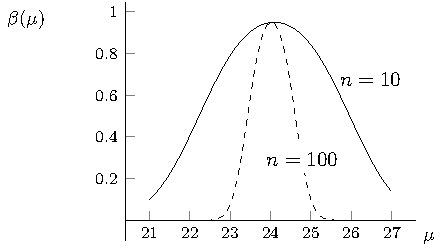
\includegraphics{normalWithKnownVarianceOperatingCharacteristics}
\caption{دو مختلف جسامت $n$ کے لئے خاصیت کارکردگی کے منحنیات۔(مثال \حوالہ{مثال_شماریات_معلوم_تغیریت_عمومی_تقسیم_کی_اوسط}-پ)}
\label{شکل_مثال_شماریات_معلوم_تغیریت_عمومی_تقسیم_کی_اوسط_کارکردگی}
\end{figure}
\انتہا{مثال}
%==================

\ابتدا{مثال}\شناخت{مثال_شماریات_نا_معلوم_تغیریت_عمومی_تقسیم_اوسط_کا_پرکھ}\quad \موٹا{نا معلوم تغیریت کی عمومی تقسیم کی اوسط کا پرکھ}\\
رسی کی تنشی مضبوطی \عددی{n=16} کا نمونہ لے کر ناپی گئی۔نمونی اوسط \عددی{\overline{x}=\SI{4482}{\kilo\gram}} اور نمونی معیاری انحراف \عددی{s=\SI{115}{\kilo\gram}} حاصل ہوئے۔ ہم فرض کرتے ہیں کہ تنشی مضبوطی عمومی بلا منصوبہ  متغیر ہے۔ قیاس \عددی{\mu_0=\SI{4500}{\kilo\gram}} کو متبادل \عددی{\mu_1=\SI{4400}{\kilo\gram}} کے مقابلے میں پرکھیں۔یہاں \عددی{\mu_0} وہ قیمت ہو سکتی ہے جو پیداکار نے فراہم کی ہو جبکہ \عددی{\mu_1} سابقہ تجربات کا نتیجہ ہو سکتا ہے۔\\
حل:\quad
ہم معنی خیز سطح \عددی{\alpha=\SI{5}{\percent}} منتخب کرتے ہیں۔اگر قیاس درست ہو تب مسئلہ \حوالہ{مسئلہ_شماریات_ٹی_تقسیم_اوسط_تغیریت} کے تحت  بلا منصوبہ متغیر
\begin{align*}
T=\sqrt{n}\,\,\,\frac{\overline{X}-\mu_0}{S}=4\,\,\, \frac{\overline{X}-4500}{S}
\end{align*}
کا \عددی{t} تقسیم \عددی{n-1=15} درجہ آزادی کا ہو گا۔ فاصل قیمت \عددی{c} کو درج ذیل مساوات سے حاصل کیا جائے گا۔
\begin{align*}
P(T<c)_{\mu_0}=\alpha=0.05
\end{align*}
ضمیمہ \حوالہ{ضمیمہ_جدول} کی جدول \حوالہ{ضمیمہ_ٹی_تقسیم} سے \عددی{c=-1.75} حاصل ہو گا۔نمونہ سے \عددی{T} کی مشاہدہ سے حاصل قیمت \عددی{t=\tfrac{4(4482-4500)}{115}=-0.626} ہے۔ہم دیکھتے ہیں کہ \عددی{t>c} ہے لہٰذا ہم قیاس کو نا منظور نہیں کرتے ہیں۔پرکھ کی طاقت کی اعدادی قیمتیں حاصل کرنے کی خاطر ہمیں مزید جدول بند قیمتیں درکار ہوں گی جن پر اس کتاب میں غور نہیں کیا جائے گا۔
\انتہا{مثال}
%=========================
\ابتدا{مثال}\شناخت{مثال_شماریات_عمومی_تقسیم_پرکھ_تغیریت}\quad \موٹا{(عمومی تقسیم کی تغیریت کی پرکھ)}\\
عمومی آبادی کے \عددی{n=15} جسامت اور نمونی تغیریت \عددی{s^2=13}  کے نمونہ سے قیاس \عددی{\sigma^2=\sigma^2_0=10} کو متبادل
 \عددی{\sigma^2=\sigma^2_1=20} میں مقابلے میں پرکھیں۔\\
حل:\quad
ہم معنی خیز سطح \عددی{\alpha=\SI{5}{\percent}} منتخب کرتے ہیں۔اگر قیاس درست ہو تب 
\begin{align*}
Y=(n-1)\frac{S^2}{\sigma^2_0}=14\frac{S^2}{10}=1.4S^2
\end{align*}
کا مربع خا تقسیم \عددی{n-1=14} درجہ آزادی کا ہو گا (مسئلہ \حوالہ{مسئلہ_شماریات_مربع_خا_تقسیم_کا_درجہ_آزادی})۔ضمیمہ \حوالہ{ضمیمہ_جدول} کی جدول \حوالہ{ضمیمہ_مربع_خا_تقسیم} اور درج ذیل سے  \عددی{14} درجہ آزادی کے لئے   \عددی{c=23.68} حاصل ہو گا 
\begin{align*}
P(Y>c)=\alpha=0.05\quad \implies \quad P(Y\le c)=0.95
\end{align*}
جو \عددی{Y} کی فاصل قیمت ہے۔یوں \عددی{S^2=\tfrac{\sigma^2_0 Y}{n-1}=0.714Y} کا مطابقتی فاصل قیمت \عددی{c^*=0.714\cdot 23.68=16.91} ہو گا۔چونکہ \عددی{s^2<c^*} ہے ہم قیاس کو نا منظور نہیں کرتے ہیں،

اگر متبادل درست ہو تب متغیر
\begin{align*}
Y_1=14\frac{S^2}{\sigma_1^2}=0.7S^2
\end{align*}
کے مربع خا تقسیم کا درجہ آزادی \عددی{14} ہو گا۔یوں ہمارے پرکھ کی طاقت
\begin{align*}
\eta=P(S^2>c^*)_{\sigma^2=20}=P(Y_1>0.7c^*)_{\sigma^2=20}=1-P(Y_1\le 11.84)_{\sigma^20}\approx \SI{62}{\percent}
\end{align*}
ہو گی اور ہم دیکھتے ہیں قسم دوم غلطی کا امکان (جو \عددی{\SI{38}{\percent}} ہے) بہت زیادہ ہے جس کو کم کرنے کے لئے نمونی جسامت بڑھانی ضروری ہے۔
\انتہا{مثال}
%===================
\ابتدا{مثال}\شناخت{مثال_دو_عمومی_تقسیمات_موازنہ_تغیریت}\quad \موٹا{دو عمومی تقسیمات کی تغیریت کا آپس میں موازنہ}\\
نا معلوم اوسط \عددی{\mu_1} کی عمومی تقسیم کا نمونہ \عددی{x_1,\cdots,x_{n1}} اور دوسری عمومی تقسیم جس کی اوسط \عددی{\mu_2} نا معلوم ہو کا نمونہ \عددی{y_1,\cdots,y_{n2}} استعمال کرتے ہوئے ہم قیاس \عددی{\mu_1=\mu_2} کو متبادل مثلاً \عددی{\mu_1>\mu_2}  کے مقابلے میں پرکھنا چاہتے ہیں۔تغیرات جاننا ضروری نہیں ہے لیکن انہیں ایک جیسا\حاشیہد{اگر اگلے مثال کا پرکھ واضح کرے کہ تغیرات میں واضح فرق پایا جاتا ہے تب ایک جیسے \عددی{n_1=n_2=n}، مثلاً \عددی{n>30} منتخب کرتے ہوئے اس حقیقت کو استعمال کرتے ہوئے کہ مساوات تخمیناً عمومی بلا منصوبہ متغیر، جس کی اوسط \عددی{0} اور تغیریت \عددی{1} ہے، کی مشاہدے سے حاصل قیمت ہے، اور مثال \حوالہ{مثال_شماریات_معلوم_تغیریت_عمومی_تقسیم_کی_اوسط} کی طرز پر حل کریں۔} تصور کیا جاتا ہے۔دو صورتیں عملاً اہم ہیں۔\\
\موٹا{پہلی صورت:}\quad
\ترچھا{نمونوں کی جسامت ایک جیسی ہے۔مزید پہلے نمونہ کی ہر قیمت کا دوسرے نمونہ میں مطابقتی ٹھیک ایک قیمت پایا جاتا ہے}، چونکہ مطابقتی قیمتیں ایک ہی انسان یا چیز کی بدولت پائی جاتی ہیں (\اصطلاح{جوڑی دار موازنہ}\فرہنگ{موازنہ!جوڑی دار}\حاشیہب{paired comparison}\فرہنگ{comparison!paired})؛مثال کے طور پر ایک ہی چیز کی دو مختلف طریقوں سے ناپ، یا ایک ہی جانور کی دو آنکھوں کی ناپ، یا زیادہ عمومی طور پر جہاں ہم کہہ سکتے ہیں کہ  نمونوں کی جوڑی قیمتیں  ایک جیسے انسانوں یا چیزوں (مثلاً جڑواں بھائی،  گاڑھی کے اگلے ٹائر، وغیرہ) سے حاصل کی گئی ہوں۔ تب ہم مطابقتی قیمتوں کا فرق لے کر، مثال \حوالہ{مثال_شماریات_نا_معلوم_تغیریت_عمومی_تقسیم_اوسط_کا_پرکھ} میں دی ترکیب استعمال کرتے ہوئے، اس قیاس کو پرکھیں گے کہ ان فرق کی مطابقتی آبادی  کی اوسط \عددی{0}  ہے۔  اگر ممکن ہو تب ہم اسی ترکیب کو استعمال کریں گے ورنہ ہمیں درج ذیل ترکیب استعمال کرنی ہو گی۔\\
\موٹا{دوسری صورت:}\quad
\ترچھا{دونوں نمونے غیر تابع ہیں اور ان کی جسامت مختلف ہو سکتی ہے۔} تب ہم درج ذیل طریقے سے بڑھتے ہیں۔فرض کریں کہ متبادل \عددی{\mu_1>\mu_2} ہے۔ہم معنی خیز سطح \عددی{\alpha} منتخب کرتے ہیں۔ہم نمونی اوسط \عددی{\overline{x}}، \عددی{\overline{y}} اور \عددی{(n_1-1)s_1^2}، \عددی{(n-1)s_2^2} کا حساب کرتے ہیں جہاں \عددی{s_1^2} اور \عددی{s_2^2} نمونی تغیریت ہیں۔ضمیمہ \حوالہ{ضمیمہ_جدول} کی جدول \حوالہ{ضمیمہ_ٹی_تقسیم} میں \عددی{n_1+n_2-2} درجہ آزادی لیتے ہوئے ہم \عددی{c} کو
\begin{align}\label{مساوات_مثال_معنی_خیز_سطح_الف}
P(T\le c)=1-\alpha
\end{align}
سے تعین کرتے ہیں۔آخر میں ہم درج ذیل کا حساب کرتے ہیں۔
\begin{align}\label{مساوات_مثال_معنی_خیز_سطح_ب}
t_0=\sqrt{\frac{n_1n_2(n_1+n_2-2)}{n_1+n_2}}\,\,\, \frac{\overline{x}-\overline{y}}{\sqrt{(n_1-1)s_1^2+(n_2-1)s_2^2}}
\end{align}
یہ دکھایا جا سکتا ہے کہ اگر قیاس درست ہو تب یہ  \عددی{t} تقسیم کے  \عددی{n_1+n_2-2} درجہ آزادی کے  بلا منصوبہ متغیر کی مشاہدے سے حاصل قیمت ہے۔اگر \عددی{t_0\le c} ہو تب قیاس کو نا منظور نہیں کیا جاتا ہے۔اگر \عددی{t_0>c}ہو تب قیاس کو نا منظور کیا جاتا ہے۔

اگر متبادل \عددی{\mu_1 \ne \mu_2} ہو تب مساوات \حوالہ{مساوات_مثال_معنی_خیز_سطح_الف} کی جگہ درج ذیل استعمال کیا جائے گا۔
\begin{align*}\tag*{(*\ref{مساوات_مثال_معنی_خیز_سطح_الف})}
P(T\le c_1)=0.5\alpha,\quad P(T\le c_2)=1-0.5\alpha
\end{align*}
دھیان رہے کہ ایک جیسی نمونی جسامت \عددی{n_1=n_2=n} کے لئے  مساوات \حوالہ{مساوات_مثال_معنی_خیز_سطح_ب} درج ذیل صورت اختیار کرتی ہے۔
\begin{align}\label{مساوات_مثال_معنی_خیز_سطح_پ}
t_0=\sqrt{n}\,\,\,\frac{\overline{x}-\overline{y}}{\sqrt{s_1^2-s_2^2}}
\end{align}

اس کی وضاحت کے لئے آئیں درج ذیل دو نمونوں پر غور کرتے ہیں جو دو مختلف حالات  میں ایک ہی کام پر مزدور کی کارکردگی ہے۔
\begin{align*}
\begin{array}{rrrrrrrr}
105&108&86&103&103&107&124&105\\
89&92&84&97&103&107&111&97
\end{array}
\end{align*}
فرض کریں کہ مطابقتی آبادی عمومی ہے اور ان کی تغیریت ایک جیسی ہے۔آئیں قیاس \عددی{\mu_1=\mu_2} کو متبادل \عددی{\mu_1\ne \mu_2} کے مقابلے میں پرکھیں۔ (تغیریت کی ایک جیسا ہونے کو اگلی مثال میں استعمال کیا جائے گا۔)\\
\موٹا{حل:}\quad
ہم درج ذیل حاصل کرتے ہیں۔
\begin{align*}
\overline{x}=105.125,\quad \overline{y}=97.500,\quad s_1^2=106.125,\quad s_2^2=84.000
\end{align*}
ہم معنی خیز سطح \عددی{\alpha=\SI{5}{\percent}} منتخب کرتے ہیں۔مساوات \حوالہ{مساوات_مثال_معنی_خیز_سطح_الف}* میں \عددی{0.5\alpha=\SI{2.5}{\percent}}، \عددی{1-0.5\alpha=\SI{97.5}{\percent}} اور  ضمیمہ \حوالہ{ضمیمہ_جدول} کی جدول \حوالہ{ضمیمہ_ٹی_تقسیم} میں \عددی{14} درجہ آزادی سے \عددی{c_1=-2.15} اور \عددی{c_2=2.15} حاصل ہوتے ہیں۔مساوات \حوالہ{مساوات_مثال_معنی_خیز_سطح_پ} میں \عددی{n=8} استعمال کرتے ہوئے درج ذیل قیمت حاصل ہوتی ہے۔
\begin{align*}
t_0=\frac{\sqrt{8}\cdot 7.625}{\sqrt{190.125}}=1.56
\end{align*}
چونکہ \عددی{c_1\le t_0\le c_2} ہے ہم دونوں صورتوں میں ایک جیسی اوسط کے  قیاس \عددی{\mu_1=\mu_2} کو نا منظور نہیں کرتے ہیں۔

پہلی صورت اس مثال پر لاگو ہوتی ہے چونکہ پہلی دونوں نمونوں کی پہلی نمونی قیمت ایک قسم کے کام کے لئے حاصل کی گئی۔اسی طرح دونوں نمونوں کی دوسری نمونی قیمت کسی دوسرے کام کے لئے حاصل کی گئی، وغیرہ۔یوں ہم ان نمونی قیمتوں کا مطابقتی فرق
\begin{align*}
\begin{array}{rrrrrrrr}
16&16&2&6&0&0&13&8
\end{array}
\end{align*}
اور مثال \حوالہ{مثال_شماریات_نا_معلوم_تغیریت_عمومی_تقسیم_اوسط_کا_پرکھ} کی ترکیب استعمال کرتے ہوئے قیاس \عددی{\mu=0} پرکھ سکتے ہیں جہاں \عددی{\mu} اس فرق کی اوسط ہے۔ہم اس کا منطقی متبادل \عددی{\mu \ne 0} لیتے ہیں۔نمونی اوسط \عددی{\overline{d}=7.625} اور نمونی تغیریت \عددی{s^2=45.696} ہے لہٰذا درج ذیل ہو گا۔
\begin{align*}
t=\frac{\sqrt{8}(7.625-0)}{\sqrt{45.696}}=3.19
\end{align*}
\عددی{P(T\le c_1)=\SI{2.5}{\percent}}، \عددی{P(T\le c_2)=\SI{97.5}{\percent}} اور ضمیمہ \حوالہ{ضمیمہ_جدول} کی جدول \حوالہ{ضمیمہ_ٹی_تقسیم} میں \عددی{n-1=7} درجہ آزادی سے \عددی{c_1=-2.37} اور \عددی{c_2=2.37} حاصل ہوتے ہیں لہٰذا ہم قیاس کو نا منظور کرتے ہیں چونکہ \عددی{t=3.19} معلوم شدہ \عددی{c_1} اور \عددی{c_2} کے بیچ نہیں پایا جاتا ہے۔اس طرح ہمارا موجودہ پرکھ، جو اسی نمونوں پر مبنی ہے لیکن زیادہ معلومات کو استعمال کرتا ہے، دکھاتا ہے کہ نتائج میں فرق کافی ہے۔ 
\انتہا{مثال} 
%=======================
\ابتدا{مثال}\quad \موٹا{(دو عمومی تقسیمات کی تغیریت کا موازنہ)}\\
گزشتہ مثال کے دو نمونے استعمال کرتے ہوئے قیاس \عددی{\sigma^2_1=\sigma^2_2}کو پرکھیں۔فرض کریں کہ مطابقتی آبادیاں عمومی ہیں اور تجربہ کی نوعیت سے متبادل \عددی{\sigma^2_1 >\sigma^2_2} ہو گا۔\\
\موٹا{حل:}\quad
ہم \عددی{s_1^2=106.125} اور \عددی{s_2^2=84.000} حاصل کرتے ہیں۔ہم معنی خیز سطح \عددی{\alpha=\SI{5}{\percent}} منتخب کرتے ہیں۔\عددی{P(V\le c)=1-\alpha=\SI{95}{\percent}} اور ضمیمہ \حوالہ{ضمیمہ_جدول} کی جدول \حوالہ{ضمیمہ_ایف_تقسیم} میں \عددی{(n_1-1,n_2-1)=(7,7)} درجہ آزادی  سے \عددی{c=3.79} تعین ہوتا ہے۔ہم آخر میں \عددی{v_0=\tfrac{s_1^2}{s_2^2}=1.26} حاصل کرتے ہیں۔چونکہ \عددی{v_0\le c} ہے ہم قیاس کو نا منظور نہیں کرتے ہیں۔اگر \عددی{v_0>c} ہوتا ہم اس کو نا منظور کرتے۔

قیاس درست ہونے کی صورت میں \عددی{v_0} ایسے بلا منصوبہ متغیر کی مشاہدے سے حاصل قیمت ہے جس کی تقسیم درجہ آزادی \عددی{(n_1-1,n_2-1)} کی \عددی{F} \اصطلاح{تقسیم}\فرہنگ{تقسیم!ایف}\حاشیہب{F-distribution}\فرہنگ{distribution!F} ہے۔  \عددی{(m,n)} درجہ آزادی کے \عددی{F} تقسیم\حاشیہد{انگلستانی ماہر جینیات رونلڈ ایلمر فشر [1890-1962]} کا تفاعل تقسیم درج ذیل ہے
\begin{align}\label{مساوات_شماریات_ایف_تقسیم}
F(z)=
\begin{cases}
K_{mn}\int_{0}^{z} t^{\tfrac{m-2}{2}} (mt+n)^{-\tfrac{m+n}{2}}\dif t& z\ge 0\\
0&z<0
\end{cases}
\end{align}
جہاں 
$K_{mn}=m^{\tfrac{m}{2}}n^{\tfrac{n}{2}}\tfrac{\Gamma(\tfrac{m}{2}+\tfrac{n}{2})}{\Gamma(\tfrac{m}{2})\Gamma(\tfrac{n}{2})}$
ہے۔اس کو ضمیمہ \حوالہ{ضمیمہ_جدول} کی جدول \حوالہ{ضمیمہ_ایف_تقسیم} میں پیش کیا گیا ہے۔
\انتہا{مثال}
%===========================

\حصہء{سوالات}
%==================
\ابتدا{سوال}\شناخت{سوال_شماریات_سکہ_منصفانہ_الف}\quad 
صفحہ \حوالہصفحہ{جدول_شماریات_سکہ_پھینکنے_کے_نتائج} پر جدول \حوالہ{جدول_شماریات_سکہ_پھینکنے_کے_نتائج} میں امجد کے مواد کو استعمال کرتے ہوئے اس قیاس کو پرکھیں کہ سکہ منصفانہ ہے، یعنی خط اور شیر کا احتمال ایک جیسا ہے۔\عددی{\alpha=\SI{5}{\percent}} منتخب کریں۔\\
جواب:\quad
اگر قیاس \عددی{p=0.5} درست ہو تب "\عددی{4040} کوششوں میں خط کی تعداد\عددی{X=}" تقریباً عمومی ہو گی جس کی اوسط \عددی{\mu=2020} اور تغیریت \عددی{\sigma^2=1010} ہو گی (حصہ \حوالہ{حصہ_شماریات_عمومی_تقسیم})۔\\
$P(X\le c)=\Phi(\tfrac{c-2020}{\sqrt{1010}})=0.95,\,\,\,c=2072>2048$
ہے لہٰذا قیاس نا منظور نہ کریں۔
\انتہا{سوال}
%=====================
\ابتدا{سوال}\quad
مشرف کا مواد استعمال کرتے ہوئے سوال \حوالہ{سوال_شماریات_سکہ_منصفانہ_الف} کو دوبارہ حل کریں۔
\انتہا{سوال}
%======================
\ابتدا{سوال}\شناخت{سوال_شماریات_قیاس_منظور_یا_نا_منظور_الف}\quad
عمومیت تصور کرتے ہوئے اور \عددی{\sigma^2=4} لیتے ہوئے قیاس \عددی{\mu=15.0} کو متبادل (الف) \عددی{\mu=12.0} اور (ب) \عددی{\mu=15.8} کے بالمقابل پرکھیں۔نمونی جسامت \عددی{10} اور نمونی اوسط \عددی{\overline{x}=14} لیں جبکہ \عددی{\alpha=\SI{5}{\percent}} منتخب کریں۔\\
جواب:\quad (الف) \عددی{c=13.96>12.00} ہے۔ قیاس کو نا منظور کریں۔\\
(ب) \عددی{c=16.04>15.80} ہے۔قیاس کو نا منظور نہ کریں۔
\انتہا{سوال}
%=========================
\ابتدا{سوال}\quad
اگر بڑی نمونی جسامت، مثلاً \عددی{100}، استعمال کی جائے تب سوال \حوالہ{سوال_شماریات_قیاس_منظور_یا_نا_منظور_الف} میں باقی مواد (\عددی{\overline{x}=14}، \عددی{\alpha=\SI{5}{\percent}}، وغیرہ) تبدیل کیے بغیر نتیجے میں کیا تبدیلی پیدا ہو گی؟ 
\انتہا{سوال}
%=============================
\ابتدا{سوال}\quad
دو طرفہ پرکھ، \عددی{\SI{5}{\percent}} سطح پر استعمال کرتے ہوئے سوال \حوالہ{سوال_شماریات_قیاس_منظور_یا_نا_منظور_الف} میں خطہ نا منظوری تلاش کریں؟\\
جواب:\quad \عددی{\mu<13.76} یا \عددی{\mu>16.24}
\انتہا{سوال}
%============================
\ابتدا{سوال}\quad
سوال \حوالہ{سوال_شماریات_قیاس_منظور_یا_نا_منظور_الف}-الف میں پرکھ کی طاقت تلاش کریں۔
\انتہا{سوال}
%=====================
\ابتدا{سوال}\quad
مثال \حوالہ{مثال_شماریات_معلوم_تغیریت_عمومی_تقسیم_کی_اوسط}-الف اور ب کی خاصیت کارکردگی کو ترسیم کریں۔  
\انتہا{سوال}
%======================
\ابتدا{سوال}\quad
دکھائیں کہ عمومی تقسیم میں قیاس \عددی{H_0:\mu=\mu_0} اور متبادل \عددی{H_1:\mu=\mu_1} کی پرکھ میں  دو اقسام کی غلطیوں کو نمونی جسامت کافی بڑھا کر  جتنا چاہیں کم (ما سوائے صفر کرنے کے) کیا جا سکتا ہے۔
\انتہا{سوال}
%=========================
\ابتدا{سوال}\شناخت{سوال_شماریات_ٹلسٹار}\quad
\عددی{\mu=0} کو \عددی{\mu>0} کے بالمقابل سطح \عددی{\alpha=\SI{5}{\percent}} پرکھیں۔ عمومیت فرض کرتے ہوئے نمونہ \عددی{1,-1,1,3,-8,6,0} لیں جو مصنوعی سیارہ \موٹا{ٹلسٹار} کی \عددی{143} ویں گردش میں مدار سے مضرب \عددی{0.01} ریڈیئن انحراف ہے۔\\
جواب:\quad
$t=\sqrt{7}\tfrac{0.286-0}{4.31}=0.18<c=1.94$
ہے لہٰذا قیاس کو نا منظور نہ کریں۔
\انتہا{سوال}
%==========================
\ابتدا{سوال}\quad
مثال \حوالہ{مثال_شماریات_اوسط} میں دیا گیا نمونہ استعمال کرتے ہوئے قیاس \عددی{\mu=\SI{0.80}{\centi\meter}} (ڈبے پر درج لمبائی) کو متبادل \عددی{\mu\ne \SI{0.80}{\centi\meter}} کے مقابل پرکھیں۔ (عمومیت تصور کرتے ہوئے \عددی{\alpha=\SI{5}{\percent}} لیں۔)
\انتہا{سوال}
%====================
\ابتدا{سوال}\quad
ایک مشین ڈبوں میں فی ڈبہ \عددی{\SI{1000}{\gram}} تیل بھرتی ہے۔آپ جاننا چاہتے ہیں کہ آیا \عددی{\alpha=\SI{5}{\percent}} سطح پر اوسط کی درکار کمیت \عددی{\SI{1000}{\gram}} سے  تجاوز زیادہ ہے۔اگر ایسا ہو تب مشین میں مطابقت پیدا کرنی ہو گی۔ایک قیاس اور متبادل  بنائیں اور انہیں پرکھیں۔ عمومیت فرض کرتے ہوئے نمونی جسامت \عددی{20} جس کی  اوسط \عددی{\SI{996}{\gram}} اور معیاری انحراف \عددی{\SI{5}{\gram}}  ہو استعمال کریں۔\\
جواب:\quad
متبادل \عددی{\mu\ne 1000}،
$t=\sqrt{20}\tfrac{996-1000}{5}=-3.58<c=-2.09$
(ضمیمہ \حوالہ{ضمیمہ_جدول} جدول  \حوالہ{ضمیمہ_ٹی_تقسیم} درجہ آزادی \عددی{19})۔ قیاس \عددی{\mu=\SI{1000}{\gram}} کو نا منظور کریں۔
\انتہا{سوال}
%======================
\ابتدا{سوال}\quad
ایک مخصوص ٹائر کی اوسط زندگی \عددی{\SI{32000}{\kilo\meter}} اور معیاری انحراف \عددی{\SI{4000}{\kilo\meter}} ہے۔کیا ٹائر کا پیداکار یہ دعویٰ کر سکتا ہے کہ اس کے بنائے ہوئے ٹائروں کی اوسط زندگی \عددی{\SI{30000}{\kilo\meter}} سے زیادہ ہے۔متبادل قیاس بناتے ہوئے اس کو \عددی{\SI{5}{\percent}} سطح پر پرکھیں۔
\انتہا{سوال}
%=====================
\ابتدا{سوال}\quad
برقی دباو کو بیک وقت دو عدد وولٹ پیما سے ناپا جاتا ہے۔ ان کے نتائج میں فرق 
\begin{align*}
0.8,0.2,-0.3,0.1,0.0,0.5,0.2
\end{align*}
 وولٹ  ہے۔عمومیت فرض کرتے ہوئے کیا ہم \عددی{\SI{5}{\percent}} سطح کے لحاظ سے وثوق سے کہہ سکتے ہیں کہ دونوں وولٹ پیما کی \ترچھا{پیمانہ بندی}\حاشیہب{calibration} میں کوئی معنی خیز فرق نہیں پایا جاتا ہے۔\\
جواب:\quad
\عددی{\mu=0} کو متبادل \عددی{\mu \ne 0} کے مقابلے میں پرکھیں۔
$t=2.11<c=2.37$
(درجہ آزادی \عددی{7})۔ قیاس کو نا منظور نہ کریں۔
\انتہا{سوال}
%=========================
\ابتدا{سوال}\quad
ایک معیاری دوائی ایک مخصوص مرض  میں مبتلا \عددی{\SI{70}{\percent}} مریضوں کو صحتیاب کرتی ہے اور ایک نئی دوائی پہلے \عددی{200} مریضوں میں سے \عددی{148} کو صحتیاب کرتی ہے۔  کیا \عددی{\alpha=\SI{5}{\percent}} لیتے ہوئے ہم وثوق سے کہہ سکتے ہیں کہ نئی دوائی زیادہ بہتر ہے؟
\انتہا{سوال}
%========================
\ابتدا{سوال}\quad
ماضی میں ایک مشین جو فی ڈبہ \عددی{\SI{25}{\kilo\gram}} چینی بھرتی تھی کا معیاری انحراف \عددی{\SI{0.4}{\kilo\gram}} تھا۔قیاس \عددی{H_0:\sigma=0.4} کو متبادل \عددی{H_1:\sigma>0.4}  کے بالمقابل پرکھیں۔عمومیت تصور کرتے ہوئے   نمونی جسامت \عددی{10}  جس کی معیاری انحراف \عددی{\sigma=0.4} ہو لیں اور 
\عددی{\alpha=\SI{5}{\percent}} منتخب کریں۔\\
جواب:\quad
$\alpha=\SI{5}{\percent}, c=16.92>\tfrac{9\cdot 0.5^2}{0.4^2}=14.06$
 ہے۔ قیاس کو نا منظور نہ کریں۔
\انتہا{سوال}
%=========================
\ابتدا{سوال}\quad
فرض کریں کہ معیاری انحراف کسی مخصوص حد سے کم، مثلاً، \عددی{5} گھنٹوں سے کم، ہونے کی صورت میں بیٹری سے چلنے والی مشینوں میں تمام بیٹریوں کو مخصوص مدت کے بعد بیک وقت تبدیل کرنا کم مہنگا پڑتا ہے  بہ نسبت ہر بیٹری کو اس وقت تبدیل کرنے کے جب وہ خراب ہو جائے۔ ایک موزوں پرکھ بنا کر اس قیاس کو پرکھیں۔عرصہ زندگی کے \عددی{28} قیمتیں جن کا معیاری انحراف \عددی{s=3.5} گھنٹے ہو استعمال کرتے ہوئے \عددی{\alpha=\SI{5}{\percent}} لیں۔عمومیت تصور کریں۔
\انتہا{سوال}
%===========================
\ابتدا{سوال}\quad
تیل کی قسم \عددی{A} کو \عددی{9} ایک جیسی گاڑیوں میں ایک جیسے حالات میں استعمال کیا گیا جنہوں نے اوسط \عددی{20.2} کلومیٹر فی لٹر اور معیاری انحراف \عددی{0.5} دیا۔انہیں حالات میں تیل کی بہتر قسم \عددی{B} کو اس جیسی \عددی{10} گاڑیوں میں استعمال کیا گیا جن سے اوسط \عددی{21.8} اور معیاری انحراف \عددی{0.6} حاصل ہوا۔کیا \عددی{B} بہت بہتر نتائج دیتا ہے؟اس قیاس کو \عددی{\alpha=\SI{5}{\percent}} پر پرکھیں۔عمومیت فرض کریں۔\\
جواب:\quad
$t_0=\sqrt{\tfrac{10\cdot9\cdot17}{19}}\tfrac{21.8-20.2}{\sqrt{9\cdot 0.6^2+8\cdot0.5^2}}=6.3>c=1.74$
(درجہ آزادی \عددی{17} ہے۔)
\انتہا{سوال}
%=======================
\ابتدا{سوال}\quad
ماسوائے عرصہ زندگی، بلب \عددی{A} اور \عددی{B}  ایک جیسے ہیں۔ایک خریدار دونوں قسم کے \عددی{100} بلب کو پرکھتا ہے۔قسم \عددی{A} کی  اوسط عرصہ زندگی \عددی{\SI{1120}{\hour}} اور معیاری انحراف \عددی{\SI{75}{\hour}} جبکہ \عددی{B} کی اوسط \عددی{\SI{1064}{\hour}} اور معیاری انحراف \عددی{\SI{82}{\hour}} حاصل ہوتے ہیں۔ کیا عرصہ زندگی میں معنی خیز فرق پایا جاتا ہے؟ (عمومیت فرض کرتے ہوئے \عددی{\alpha=\SI{5}{\percent}} سطح پر پرکھیں۔)
\انتہا{سوال}
%===========================
\ابتدا{سوال}\quad
نمونی جسامت \عددی{10} اور \عددی{16} اور تغیریت \عددی{s_1^2=50} اور \عددی{s_2^2=30} لیں۔ عمومیت تصور کرتے ہوئے \عددی{\alpha=\SI{5}{\percent}} سطح پر  قیاس \عددی{H_0:\sigma^2_1=\sigma_2^2} کو متبادل \عددی{H_1:\sigma^2_1>\sigma^2_2} کے بالمقابل پرکھیں۔\\
جواب:\quad
$v_0=\tfrac{50}{30}=1.67<c=2.59$
[درجہ آزادی \عددی{(9,15)} ہے۔] قیاس کو نا منظور نہ کریں۔
\انتہا{سوال}
%=============================
\ابتدا{سوال}\quad
دو نمونے \عددی{50,90,100,90,110,80} اور \عددی{110,110,120,110,130,110,120} لوہے کی ڈھلائی کے دوران دو مختلف بالٹیوں میں دو مختلف وقتوں پر درجہ حرارت \عددی{(\si{\celsius})} میں فرق دیتی ہیں۔ کیا پہلے نمونہ کی تغیریت دوسرے  سے زیادہ ہے؟ عمومیت فرض کریں اور \عددی{\alpha=\SI{5}{\percent}} لیں۔
\انتہا{سوال}
%=========================

\حصہ{ضبط معیار}
پیداوار کا کوئی بھی عمل اتنا ٹھیک نہیں ہوتا ہے کہ تمام پیداوار مکمل طور پر ایک جیسی ہو۔  بہت ساری معمولی، غیر قابو وجوہات کی بنا ان میں ہر صورت معمولی فرق پایا جاتا ہے جس کو امکانی فرق تصور کیا جا سکتا ہے۔یہ ضروری ہے کہ پیداوار کی درکار خاصیت کی قیمت درست ہو (مثلاً لمبائی، مضبوطی، یا جو بھی خاصیت کسی مخصوص صورت میں درکار ہو)۔ اس مقصد کے لئے اس قیاس کو پرکھا جاتا ہے کہ پیداوار درکار خاصیت، مثلاً \عددی{\mu=\mu_0}، رکھتے ہیں جہاں \عددی{\mu_0} درکار قیمت ہے۔اگر ایسا پوری کھیپ کی پیداوار (مثلاً، \عددی{100000} پیچوں کی کھیپ) کے بعد کیا جائے تب پرکھ ہمیں بتائے گا کہ  پیداوار کتنی اچھی یا کتنی خراب ہے لیکن ظاہر ہے کہ اس نتیجہ کو استعمال کرتے ہوئے ہم کوئی بہتری نہیں لا سکتے ہیں۔بہتری لانے کے لئے ضروری ہے کہ پرکھ دوران پیداوار کیا جائے۔ایسا عموماً مقررہ دورانیہ (مثلاً ہر \عددی{30} منٹ یا ہر گھنٹہ) بعد جاتا ہے اور اس کو \اصطلاح{ضبط معیار}\فرہنگ{ضبط معیار}\فرہنگ{معیار!ضبط}\حاشیہب{quality control}\فرہنگ{control!quality} کہتے ہیں۔ہر مرتبہ ایک جیسی جسامت (عملاً \عددی{3} یا \عددی{10} اجزاء) کا نمونہ لیا جاتا ہے۔قیاس نا منظور ہونے کی صورت میں عمل پیداوار روک کر اس وجہ کو تلاش کیا جاتا ہے جس کی بنا انحراف پیدا ہوا ہے۔

اگر ہم عمل پیدا وار کو روک دیں اگرچہ سب ٹھیک چل رہا ہو تب ہم غلطی قسم اول  کر رہے ہوں گے۔اگر خرابی کے باوجود ہم عمل پیداوار کو نا روکیں تب ہم غلطی قسم دوم  کر رہے ہوں گے (حصہ \حوالہ{حصہ_شماریات_قیاس_کی_پرکھ_فیصلے})۔

ہر پرکھ کا نتیجہ کو ترسیمی صورت میں \اصطلاح{نقشہ ضبط}\فرہنگ{ضبط!نقشہ}\حاشیہب{control chart}\فرہنگ{control!chart} پر ظاہر\حاشیہد{امریکی ماہر شماریات والٹر انڈرو شوہارٹ [1891-1967] نے یہ نقشہ  \سن{1924} میں تجویز کیا جو معیار کو قابو کرنے میں انتہائی موثر ثابت ہوا ہے۔} کیا جاتا ہے۔

\جزوحصہء{اوسط کا نقشہ ضبط}
شکل \حوالہ{شکل_شماریات_نقش_ضبط} میں نقشہ ضبط کی مثال دکھائی گئی ہے۔اوسط کے نقشہ ضبط پر \اصطلاح{نچلی حد ضبط}\فرہنگ{ضبط!نچلی حد}\حاشیہب{lower control limit ($\LCL$)}\فرہنگ{control!lower limit} \عددی{\LCL}، \اصطلاح{وسطی خط ضبط}\فرہنگ{ضبط!وسطی خط}\حاشیہب{central control line ($\CL$)}\فرہنگ{control!central line} \عددی{\CL} اور \اصطلاح{بالائی حد ضبط}\فرہنگ{ضبط!بالائی حد}\حاشیہب{upper control limit ($\UCL$)}\فرہنگ{control!upper limit} \عددی{\UCL} دکھائے گئے ہیں۔ یہ  حدود مثال \حوالہ{مثال_شماریات_معلوم_تغیریت_عمومی_تقسیم_کی_اوسط}-پ میں فاصل قیمتوں \عددی{c_1} اور \عددی{c_2} کے مطابقتی ہیں۔جیسے ہم نمونی اوسط نچلی حد ضبط یا بالائی حد ضبط سے تجاوز کر جائے ہم قیاس کو نا منظور کرتے ہوئے کہتے ہیں کہ عمل پیداوار "بے قابو" ہے، یعنی، ہم کہتے ہیں کہ عمل پیداوار میں تبدیلی رو نما ہوئی ہے۔جب بھی کوئی نقطہ حدود ضبط سے تجاوز کرے عمل پیداوار میں مداخلت کی ضرورت ہو گی۔

اگر ہم حدود ضبط ڈھیلے  رکھیں تب ہم عمل پیداوار میں نا پسندیدہ تبدیلی کو پکڑ نہیں پائیں گے۔اس کے برعکس حدود ضبط بہت سخت رکھنے سے  ہم بار بار عمل پیداوار کو روک کر نا پسندیدہ تبدیلی کی  غیر موجود وجہ تلاش کرتے رہیں گے جس سے پیداوار بری طرح متاثر ہو گی۔عموماً معنی خیز سطح \عددی{\alpha=\SI{1}{\percent}} منتخب کی جاتی ہے۔صفحہ \حوالہصفحہ{مسئلہ_شماریات_عمومی_کی_شرط_اوسط_تغیریت} پر مسئلہ \حوالہ{مسئلہ_شماریات_عمومی_کی_شرط_اوسط_تغیریت} اور ضمیمہ \حوالہ{ضمیمہ_جدول} کی جدول \حوالہ{ضمیمہ_عمومی_تقسیم_ب} سے ہم دیکھتے ہیں کہ عمومی تقسیم کی صورت میں اوسط کے مطابقتی حد ضبط
\begin{align}\label{مساوات_شماریات_حدود_ضبط_عمومی_تقسیم}
\LCL=\mu_0-2.58\,\,\,\frac{\sigma}{\sqrt{n}} \quad \text{اور}\quad \UCL=\mu_0+2.58\,\,\,\frac{\sigma}{\sqrt{n}}
\end{align} 
ہوں گے۔یہاں فرض کیا گیا ہے کہ ہمیں \عددی{\sigma} معلوم ہے۔اگر \عددی{\sigma} نا معلوم ہو تب پہلی \عددی{20} یا \عددی{30} نمونوں کی معیاری انحراف  حاصل کر کے ان کی اوسط کو \عددی{\sigma} کی تخمینی قیمت تصور کیا جا سکتا ہے۔شکل \حوالہ{شکل_شماریات_نقش_ضبط} میں اوسط  کو  لکیر سے جوڑا جاتا ہے جو محض نتائج کو واضح کرنے میں مدد دیتی ہے۔


\جزوحصہء{تغیریت کا نقشہ ضبط}
اوسط کے ساتھ ساتھ عموماً تغیریت، معیاری انحراف یا سعت کو بھی قابو رکھا جاتا ہے۔عمومی تقسیم کی صورت میں معیاری انحراف کا نقشہ ضبط بناتے ہوئے مثال \حوالہ{مثال_شماریات_عمومی_تقسیم_پرکھ_تغیریت} میں استعمال ترکیب بروئے کار لاتے ہوئے حدود ضبط تعین کیے جا سکتے ہیں۔روایتی طور پر صرف بالائی حد ضبط استعمال کیا جاتا ہے۔مثال \حوالہ{مثال_شماریات_عمومی_تقسیم_پرکھ_تغیریت} سے یہ حد
\begin{align}\label{مساوات_شماریات_تغیریت_بالائی_حد_ضبط}
\UCL=\frac{\sigma^{\,\,\,2} c}{n-1}
\end{align}
ہو گا جہاں \عددی{c} کو مساوات 
\begin{align*}
P(Y>c)=\alpha \quad  \implies  \quad P(Y\le c)=1-\alpha
\end{align*}
اور ضمیمہ \حوالہ{ضمیمہ_جدول} کی جدول \حوالہ{ضمیمہ_مربع_خا_تقسیم} (مربع خا تقسیم) سے \عددی{n-1} درجہ آزادی کے لئے  حاصل کیا جاتا ہے؛ یہاں نمونہ سے مشاہدے کے ذریعہ  \عددی{S^2} کی حاصل قیمت \عددی{s^2} کا بالائی حد ضبط سے تجاوز کا احتمال \عددی{\alpha} (\عددی{\SI{5}{\percent}} یا \عددی{\SI{1}{\percent}}) ہے۔

اگر ہم تغیریت کے نقشہ ضبط میں نچلی حد ضبط  اور بالائی حد ضبط استعمال کرنا چاہیں تب یہ حدود
\begin{align}\label{مساوات_شماریات_تغیریت_دونوں_حدود}
\LCL=\frac{\sigma^2 c_1}{n-1},\quad \UCL=\frac{\sigma^2 c_2}{n-1}
\end{align} 
ہوں گے جہاں \عددی{c_1} اور \عددی{c_2} کو  \عددی{n-1} درجہ آزادی کے لئے  ضمیمہ \حوالہ{ضمیمہ_جدول} کی جدول \حوالہ{ضمیمہ_مربع_خا_تقسیم}  اور درج ذیل مساوات سے حاصل کیا جائے گا۔
\begin{align}
P(Y\le c_1)=\frac{\alpha}{2},\quad P(Y\le c_2)=1-\frac{\alpha}{2}
\end{align}
%================================
\begin{figure}
\centering
\begin{subfigure}{1\textwidth}
\centering
\begin{tikzpicture}
\draw(0,-2)--(0,2);
\foreach \x in {1,2,3,4,5,6,7,8,9,10,11,12,13,14}{\draw[gray](\x/2.5,-2)--++(0,4);}
\foreach \y in {1,2,3,4,6,7,8,9}{\draw[gray](0,\y/5)--++(5.6,0) (0,-\y/5)--++(5.6,0);}
\draw(0,0/5)node[left]{$4.10$}--++(5.6,0);
\draw(0,5/5)node[left]{$4.15$}--++(5.6,0);
\draw[gray](0,10/5)node[left,black]{$4.20$}--++(5.6,0);
\draw(0,-5/5)node[left]{$4.05$}--++(5.6,0);
\draw[gray](0,-10/5)node[left,black]{$4.00$}--++(5.6,0);
\draw(5/2.5,-10/5)node[below]{$5$};
\draw(10/2.5,-10/5)node[below]{$10$};
\draw(5.6,5/5)node[right]{\RL{بالائی حد ضبط}};
\draw(5.6,0/5)node[right]{\RL{وسطی خط ضبط}};
\draw(5.6,-5/5)node[right]{\RL{نچلی حد ضبط}};
\draw(6.8,5/5)--++(0.85,0);
\draw(6.8,-5/5)--++(0.85,0);
\draw(1/2.5,20*4.080-20*4.10)node[ocirc]{}
\foreach \x/\y in {2/4.112,3/4.084,4/4.088,5/4.108,6/4.100,7/4.088,8/4.096,9/4.100,10/4.104,11/4.140,12/4.152}{--(\x/2.5,20*\y-20*4.10)node[ocirc]{}};
\draw[stealth-stealth] (7.54,5/5)--++(0,-2)node[pos=0.5,fill=white]{$\SI{99}{\percent}$};
\draw[stealth-] (7.54,5/5)--++(0,1)node[pos=0.5,fill=white]{$\SI{0.5}{\percent}$};
\draw[stealth-] (7.54,-5/5)--++(0,-1)node[pos=0.5,fill=white]{$\SI{0.5}{\percent}$};
\draw(-1,0.5)node[rotate=90]{اوسط};
\draw(3,-2)node[below]{\RL{شمار نمونہ}};
\end{tikzpicture}
\end{subfigure}
\begin{subfigure}{1\textwidth}
\centering
\begin{tikzpicture}
\draw(0,0)--(0,4);
\foreach \x in {1,2,3,4,5,6,7,8,9,10,11,12,13,14}{\draw[gray](\x/2.5,0)--++(0,4);}
\foreach \y in {0,1,2,3,4,5,6,7,8}{\draw[gray](0,\y/2)--++(5.6,0);}
\draw(0,2)node[left]{$0.02$}--++(5.6,0);
\draw(0,100*0.036)node[left]{$0.036$}--++(5.6,0);
\draw(0,0)node[left]{$0$};
\draw(0,100*0.01)node[left]{$0.01$};
\draw(0,100*0.03)node[left]{$0.03$};
\draw(0,100*0.04)node[left]{$0.04$};
\draw(5/2.5,0)node[below]{$5$};
\draw(10/2.5,0)node[below]{$10$};
%curve
\draw(1/2.5,100*0.014)node[ocirc]{}
\foreach \x/\y in{2/0.011,3/0.026,4/0.023,5/0.018,6/0.014,7/0.023,8/0.017,9/0.032,10/0.038}{--(\x/2.5,100*\y)node[ocirc]{}};
\draw(-1,2)node[rotate=90]{\RL{معیاری انحراف}};
\draw(3,0)node[below]{\RL{شمار نمونہ}};
\draw(5.6,3.65)node[right]{\RL{بالائی حد ضبط}};
\draw(6.8,3.65)--++(0.85,0);
\draw(6.5,0)--(7.65,0);
\draw[stealth-stealth] (7.54,0)--++(0,3.65)node[pos=0.5,fill=white]{$\SI{99}{\percent}$};
\draw[stealth-] (7.54,3.65)--++(0,1)node[pos=0.5,fill=white]{$\SI{1}{\percent}$};
\end{tikzpicture}
\end{subfigure}
\caption{اوسط اور معیاری انحراف کے نقشہ ضبط برائے جدول \حوالہ{جدول_شماریات_نلکی_کے_قطر_کا_نمونہ}}
\label{شکل_شماریات_نقش_ضبط}
\end{figure}

%====================
\جزوحصہء{معیاری انحراف کا نقشہ ضبط}
تغیریت کے نقشہ ضبط کی طرح ہمیں بالائی حد ضبط
\begin{align}\label{مساوات_شماریات_معیاری_انحراف_بالائی_حد}
\UCL=\frac{\sigma \sqrt{c}}{\sqrt{n-1}}
\end{align}
درکار ہو گا جس کو مساوات \حوالہ{مساوات_شماریات_تغیریت_بالائی_حد_ضبط} سے حاصل کیا گیا ہے۔مثال کے طور پر جدول \حوالہ{جدول_شماریات_نلکی_کے_قطر_کا_نمونہ} میں \عددی{n=5} ہے۔مطابقتی آبادی کو عمومی تصور کرتے ہوئے جس کی معیاری انحراف \عددی{\sigma=0.02} ہو، \عددی{\alpha=\SI{1}{\percent}}  منتخب کرتے ہوئے  \عددی{4} درجہ آزادی کے لئے  ضمیمہ \حوالہ{ضمیمہ_جدول} کی جدول \حوالہ{ضمیمہ_مربع_خا_تقسیم} اور مساوات
\begin{align*}
P(Y\le c)=1-\alpha=\SI{99}{\percent}
\end{align*}
سے فاصل قیمت \عددی{c=13.28} حاصل ہوتی ہے۔یوں مساوات \حوالہ{مساوات_شماریات_معیاری_انحراف_بالائی_حد} سے
\begin{align*}
\UCL=\frac{0.02\sqrt{13.28}}{\sqrt{4}}=0.0365
\end{align*}
حاصل ہو گا جس کو شکل \حوالہ{شکل_شماریات_نقش_ضبط} کے نچلے حصے میں دکھایا گیا ہے۔

معیاری انحراف کا نقشہ ضبط جس میں بالائی حد ضبط اور نچلا حد ضبط پائے جاتے ہوں کو مساوات \حوالہ{مساوات_شماریات_تغیریت_دونوں_حدود} سے حاصل کیا جا سکتا ہے۔

\begin{table}
\caption{بارہ نمونے جہاں ہر نمونہ $5$ قیمتوں (چھوٹی نلکیوں کے ملی میٹروں میں قطر) پر مشتمل ہے}
\label{جدول_شماریات_نلکی_کے_قطر_کا_نمونہ}
\centering
\begin{otherlanguage}{english}
\begin{tabular}{C|CCCCC|C|C|C}
\hline
\text{\RL{\urdufont{نمونی شمار}}} & \multicolumn{5}{C|}{\text{\RL{\urdufont{نمونی قیمتیں}}}}& \overline{x}&s&R\\
\hline
1&4.06&4.08&4.08&4.08&4.10&4.080&0.014&0.04\\
2&4.10&4.10&4.12&4.12&4.12&4.112&0.011&0.02\\
3&4.06&4.06&4.08&4.10&4.12&4.084&0.026&0.06\\
4&4.06&4.08&4.08&4.10&4.12&4.088&0.023&0.06\\
5&4.08&4.10&4.12&4.12&4.12&4.108&0.018&0.04\\
&&&&&&&&\\
6&4.08&4.10&4.10&4.10&4.12&4.100&0.014&0.04\\
7&4.06&4.08&4.08&4.10&4.12&4.088&0.023&0.06\\
8&4.08&4.08&4.10&4.10&4.12&4.096&0.017&0.04\\
9&4.06&4.08&4.10&4.12&4.14&4.100&0.032&0.08\\
10&4.06&4.08&4.10&4.12&4.16&4.104&0.038&0.10\\
&&&&&&&&\\
11&4.12&4.14&4.14&4.14&4.16&4.140&0.014&0.04\\
12&4.14&4.14&4.16&4.16&4.16&4.152&0.011&0.02\\
\hline
\end{tabular}
\end{otherlanguage}
\end{table}
%======================================
\جزوحصہء{سعت کا نقشہ ضبط}
اگر ہم \عددی{\sigma^2} یا \عددی{\sigma} کو قابو رکھتے ہوں تب ہمیں بالترتیب \عددی{s^2} یا \عددی{s} کا حساب کرنا ہو گا۔ایسا کرنا  غیر تربیت یافتہ شخص کے لئے مشکل ہوتا ہے لہٰذا ہم تغیریت یا معیاری انحراف کی حد ضبط کی جگہ سعت \عددی{R=}(نمونہ کی زیادہ سے زیادہ قیمت منفی نمونہ کی کم سے کم قیمت) استعمال کرنا چاہیں گے۔عمومی تقسیم کی صورت میں یہ دکھایا جا سکتا ہے کہ معیاری انحراف \عددی{\sigma} کی قیمت بلا منصوبہ متغیر \عددی{R^*} کی  توقع  کے راست متناسب ہے جس کی مشاہدے سے حاصل قیمت \عددی{R} ہو، یعنی \عددی{\sigma=\lambda_nE(R^*)}، جہاں جزو \عددی{\lambda_n} کی قیمت نمونی جسامت پر منحصر ہے اور اس کی قیمتیں درج ذیل ہیں۔
\begin{align*}
\begin{array}{cccccccccc}
n&2&3&4&5&6&7&8&9&10\\
\hline
\lambda_n=\sigma/E(R^*)&0.89&0.59&0.49&0.43&0.40&0.37&0.35&0.34&0.32\\[1ex]
n&12&14&16&18&20&30&40&50&\\
\hline
\lambda_n=\sigma/E(R^*)&0.31&0.29&0.28&0.28&0.27&0.25&0.23&0.22&
\end{array}
\end{align*}

چونکہ \عددی{R} صرف دو نمونی قیمتوں پر منحصر ہے لہٰذا یہ نمونے کے بارے میں \عددی{s} کے لحاظ سے کم معلومات فراہم کرتا ہے۔ظاہر ہے کہ نمونی جسامت \عددی{n} جتنی بڑی ہو گی، \عددی{s} کی جگہ \عددی{R} استعمال کرنے سے، اتنی زیادہ معلومات ہم ضائع کریں گے۔عملاً اگر \عددی{n} کی قیمت \عددی{10} سے زائد ہو تب \عددی{s} استعمال کیا جاتا ہے۔

دھیان رہے کہ سعت سے  معیاری انحراف کا جلدی سے  اندازہ لگانا عملی استعمال میں کار آمد ثابت ہوتا ہے۔

%==================
\حصہء{سوالات}
  
%=====================
\ابتدا{سوال}\شناخت{سوال_شماریات_حد_ضبط_الف}\quad 
ایک مشین چکنا تیل کو ٹین کی بوتل میں یوں بھرتی ہے کہ عمومی آبادی حاصل ہو جس کی اوسط \عددی{1} لٹر اور معیاری انحراف \عددی{0.03} لٹر ہو۔ اوسط کے لئے شکل \حوالہ{شکل_شماریات_نقش_ضبط} کی طرح نقشہ درکار ہے۔ نمونی جسامت \عددی{6} فرض کرتے ہوئے نچلی حد ضبط اور بالائی حد ضبط تلاش کریں۔\\
جواب:\quad
نچلی حد ضبط 
$\LCL=1-\tfrac{2.58\cdot 0.03}{\sqrt{6}}=0.968$
جبکہ بالائی حد ضبط \عددی{\UCL=1.032}
\انتہا{سوال}
%=========================
\ابتدا{سوال}\quad
سوال \حوالہ{سوال_شماریات_حد_ضبط_الف} میں دکھائیں کہ \عددی{\alpha=\SI{0.3}{\percent}} سطح سے درج ذیل  حاصل ہوتے ہیں۔ان کی اعدادی قیمتیں تلاش کریں۔
\begin{align*}
\LCL=\mu-\tfrac{3\sigma}{\sqrt{n}},\quad \UCL=\mu+\tfrac{3\sigma}{\sqrt{n}}
\end{align*}
\انتہا{سوال}
%========================
\ابتدا{سوال}\quad
معنی خیز سطح تبدیل کیے بغیر ہمیں سوال \حوالہ{سوال_شماریات_حد_ضبط_الف} میں نمونی جسامت کتنی رکھنی ہو گی تا کہ بالائی اور نچلی حد ضبط قریب قریب ہوں، مثلاً \عددی{\UCL-\LCL=0.05}\\
جواب:\quad
$n=10$
\انتہا{سوال}
%======================
\ابتدا{سوال}\quad
اگر ہم غیر عمومی آبادی کے  لئے مساوات \حوالہ{مساوات_شماریات_حدود_ضبط_عمومی_تقسیم} کے حدود ضبط والا نقشہ ضبط استعمال کریں تب ان حدود کا کیا مطلب ہو گا؟
\انتہا{سوال}
%=============================
\ابتدا{سوال}\quad
عمومی آبادی کی اوسط قابو کرتے ہوئے  \عددی{\UCL-\LCL} کو نصف کرنے کی خاطر نمونی جسامت کو کس طرح تبدیل کرنا ہو گا؟\\
جواب:\quad
نمونی جسامت کو \عددی{4} گنا بڑھانا ہو گا۔
\انتہا{سوال}
%===========================
\ابتدا{سوال}\quad
قابلوں کی پیداوار میں سے \عددی{2} جسامت کے \عددی{10} نمونے لئے گئے۔ان کی لمبائی ملی میٹروں میں درج ذیل ہے۔
\begin{align*}
\begin{array}{ccccccccccc}
\text{\RL{نمونی شمار}}&1&2&3&4&5&6&7&8&9&10\\
\hline
\multirow{2}{*}{\text{\RL{لمبائی}}}&27.4&27.4&27.5&27.3&27.9&27.6&27.6&27.8&27.5&27.3\\
&27.6&27.4&27.7&27.4&27.5&27.5&27.4&27.3&27.4&27.7
\end{array}
\end{align*}
فرض کریں کہ آبادی عمومی ہے جس کی اوسط \عددی{27.5} اور تغیریت \عددی{0.024} ہے۔مساوات \حوالہ{مساوات_شماریات_حدود_ضبط_عمومی_تقسیم} استعمال کرتے ہوئے اوسط کے لئے نقش ضبط بنائیں اور نمونی اوسط اس پر ترسیم کریں۔\\
جواب:\quad
$\tfrac{2.58\sqrt{0.024}}{\sqrt{2}}=0.283,\UCL=27.783,\LCL=27.217$
\انتہا{سوال}
%==========================
\ابتدا{سوال}\شناخت{سوال_شماریات_موٹائی_الف}\quad
لوہے کی چادر موٹائی کے درج ذیل نمومے \عددی{30} منٹ کے وقفوں پر حاصل کیے گئے۔ان کی اوسط کو نقش ضبط پر ترسیم کریں۔فرض کریں کہ آبادی عمومی ہے جس کی اوسط \عددی{5} اور معیاری انحراف \عددی{1.55} ہے۔
\begin{align*}
\begin{array}{ccccccccccc}
\text{\RL{نمونی شمار}} &1&2&3&4&5&6&7&8&9&10\\
\hline
\multirow{4}{*}{\RL{نمونی قیمتیں}} &3&3&5&7&7&4&5&6&5&5\\
&4&6&2&5&3&4&6&4&5&2\\
&8&6&5&4&6&3&4&6&6&5\\
&4&8&6&4&5&6&6&4&4&3
\end{array}
\end{align*} 
\انتہا{سوال}
%=======================
\ابتدا{سوال}\quad
سعت کے نقشہ ضبط پر سوال \حوالہ{سوال_شماریات_موٹائی_الف} کے نمونی سعت کو ترسیم کریں۔
\انتہا{سوال}
%===========================
\ابتدا{سوال}\quad
\عددی{\lambda_n=\tfrac{\sigma}{E(R^*)}} بالمقابل \عددی{n} ترسیم کریں۔\عددی{\lambda_n} متغیر \عددی{n} کا یک سر گھٹتا تفاعل ہے۔اس کی وجہ بیان کریں۔
\انتہا{سوال}
%=============================
\ابتدا{سوال}\quad
حدود ضبط کے باہر اوسط کا نقطہ نظام میں خرابی کو ظاہر کرتی ہے۔اگر ہم (الف) \عددی{1\sigma} حد، (ب) \عددی{2\sigma} حد، منتخب کریں تب ہم کتنی بار نظام میں غیر موجود خرابی کو تلاش کرنے کی کوشش کریں گے۔(عمومیت فرض کریں۔)\\
جواب:\quad
تقریباً \عددی{\SI{30}{\percent}\,\,\,(\SI{5}{\percent})} صورتوں میں
\انتہا{سوال}
%===========================
\ابتدا{سوال}\quad
ایک خود کار خراد کی مشین پر قابلے بنائے جاتے ہیں۔ مسلسل رگڑ سے پیدا تبدیلی، اوسط کی نقش ضبط پر کس طرح رونما ہو گی؟ خراد کی مشین میں یک دم تبدیلی کس طرح نقش ضبط پر نظر آئے گی؟   
\انتہا{سوال}
%==========================
\ابتدا{سوال}\quad \موٹا{(عیب داروں کی تعداد)}\quad
\عددی{3\sigma} حدود ضبط کے لحاظ سے  \عددی{\UCL}، \عددی{\CL} اور \عددی{\LCL} کے کلیات عیب دار کے نقشہ ضبط کے لئے  تلاش کریں۔(فرض کریں کہ شماریاتی ضبط میں \عددی{p} عیب دار کو ظاہر کرتا ہے۔)\\
$\UCL=np+3\sqrt{np(1-p)},\CL=np,\LCL=np-3\sqrt{np(1-p)}$
\انتہا{سوال}
%=======================
\ابتدا{سوال}\quad \موٹا{خاصیت کی نقش ضبط} \quad
برتنوں کی پیداوار سے جسامت \عددی{100} کے نمونے حاصل کیے گئے۔عیب دار (رستا برتنوں) کی تعداد (اسی ترتیب سے) درج ذیل تھی۔
\begin{align*}
3\,\,\,7\,\,\,6\,\,\,1\,\,\,4\,\,\,5\,\,\,4\,\,\,9\,\,\,7\,\,\,0\,\,\,5\,\,\,6\,\,\,13\,\,\,4\,\,\,9\,\,\,0\,\,\,2\,\,\,1\,\,\,12\,\,\,8
\end{align*} 
گزشتہ تجربہ سے ہم جانتے ہیں کہ اگر عمل پیداوار میں خرابی نہ ہو تب  عیب دار کی اوسط تعداد \عددی{p\si{\percent}} ہوتی ہے۔ثنائی تقسیم استعمال کرتے ہوئے عیب دار نقشہ ضبط (جس کو \عددی{p} نقشہ بھی کہتے ہیں) بنائیں، یعنی، \عددی{\LCL=0} لیں اور  \عددی{3\sigma} حدود کے لئے حاصل عیب دار (فی صد)  کو \عددی{\UCL} لیں، جہاں بلا منصوبہ متغیر \عددی{=\overline{X}}\ترچھا{نمونہ میں فی صد عیب دار} کی تغیریت \عددی{\sigma^2} ہے۔کیا عمل پیداوار قابو میں ہے؟
\انتہا{سوال}
%=========================
\ابتدا{سوال}\quad \موٹا{فی اکائی عیب دار کی تعداد} \quad
فی اکائی عیب دار کے نقشہ (جس کو \عددی{c} نقشہ بھی کہتے ہیں) کو فی اکائی عیب دار \عددی{X} (مثلاً \عددی{10} میٹر کاغذ میں عیبوں کی تعداد، جہاز کے ایک پر میں غیر موجود کیلوں کی تعداد، وغیرہ) کو قابو کرنے کے لئے استعمال کیا جاتا ہے۔ (الف)   \عددی{X} کی تقسیم کو  پوئسن تقسیم تصور کرتے ہوئے  \عددی{\mu\mp 3\sigma} کے لحاظ سے \عددی{\CL}، \عددی{\LCL}  اور \عددی{\UCL} کے کلیات بنائیں۔ (ب) شیشے کی چادر میں عیب کے لئے \موٹا{عمل قابو}\فرہنگ{عمل قابو}\فرہنگ{قابو!عمل}\حاشیہب{control process}\فرہنگ{control process} کے لئے \عددی{\CL}، \عددی{\LCL} اور \عددی{\UCL} تلاش کریں؛ فرض کریں کہ جب عمل پیداوار شماریاتی قابو میں ہو تب اوسطاً یہ عدد \عددی{2.5} فی چادر ہے۔ 
\انتہا{سوال}
%=========================

\حصہ{قبولیت نمونہ}
بڑے پیمانہ پر پیداوار میں، جہاں پیداکار خریدار کو \عددی{N} اشیاء کی کھیپ مہیا کرتا ہے، قبولیت نمونہ لاگو کیا جاتا ہے۔ایسی صورت میں ہر کھیپ کو قبول یا مسترد کرنے کا فیصلہ کرنا ہو گا۔  کھیپ سے \عددی{n} جسامت کے نمونے کا معائنہ کرتے ہوئے \موٹا{عیب دار اشیاء} ، جنہیں مختصراً \اصطلاح{عیب دار}\فرہنگ{عیب دار}\حاشیہب{defectives}\فرہنگ{defectives} کہتے ہیں،  کی تعداد کو مد نظر رکھ کر عموماً  فیصلہ کیا جاتا ہے۔ جو اشیاء درکار تخصیص  (بیان کردہ خواص، مثلاً جسامت، رنگ، مضبوطی، یا جو بھی اہمیت رکھتا ہو) پر پورا نہیں اترتے ہیں، انہیں عیب دار تصور کیا جاتا ہے۔ اگر نمونہ میں عیب دار اشیاء  کی تعداد \عددی{x} طے شدہ عدد \عددی{c\, (<n)} سے زیادہ نہ ہو تب کھیپ کو قبول کیا جاتا ہے۔اگر \عددی{x>c} ہو تب کھیپ کو مسترد کیا جاتا ہے۔\عددی{c} کو \ترچھا{عیب دار کی قابل قبول تعداد} یا \اصطلاح{تعداد قبولیت}\فرہنگ{تعداد قبولیت}\حاشیہب{acceptance number}\فرہنگ{acceptance number} کہتے ہیں۔ ظاہر ہے کہ پیدا کار اور خریدار کو \اصطلاح{نمونی منصوبہ}\فرہنگ{نمونی منصوبہ}\حاشیہب{sampling plan}\فرہنگ{sampling plan}  پر اتفاق کرنا ہو گا، یعنی، نمونی جسامت \عددی{n} کی قیمت  اور تعداد قبولیت \عددی{c} کی قیمت۔چونکہ یہ ایک نمونہ پر منحصر ہے لہٰذا اس  کو \اصطلاح{واحد نمونی منصوبہ}\فرہنگ{نمونی!واحد منصوبہ}\حاشیہب{single sampling plan}\فرہنگ{sampling!single plan} کہتے ہیں۔ \اصطلاح{دوہرا نمونی منصوبہ} پر بعد میں غور کیا جائے گا۔

فرض کریں کہ کھیپ قبول ہونے کا وقوعہ \عددی{A} ہے۔ظاہر ہے کہ مطابقتی احتمال \عددی{P(A)} نا صرف \عددی{n} اور \عددی{c} بلکہ کھیپ میں عیب داروں کی تعداد \عددی{M} پر بھی منحصر ہے۔فرض کریں کہ نمونہ میں عیب داروں کی تعداد بلا منصوبہ متغیر \عددی{X} ہے اور ہم بغیر واپس رکھے  نمونہ حاصل کرتے ہیں۔ تب (حصہ \حوالہ{حصہ_شماریات_ثنائی_پوئسن_بیش_ہندسی_تقسیم})
\begin{align}\label{مساوات_شماریات_نسبت_عیب_دار_الف}
P(A)=P(X\le c)=\sum_{x=0}^{c}\frac{\binom{M}{x}\binom{N-M}{n-x}}{\binom{N}{n}}
\end{align}
ہو گا۔اگر \عددی{M=0} (کھیپ میں کوئی عیب دار نہیں ہے) ہو تب \عددی{X} کی قیمت لازماً \عددی{0} ہو گی اور
\begin{align*}
P(A)=\frac{\binom{0}{0}\binom{N}{n}}{\binom{N}{n}}=1
\end{align*}
ہو گا۔مقررہ \عددی{n} اور \عددی{c} اور بڑھتے \عددی{M} کی صورت میں احتمال \عددی{P(M)} گھٹتا ہے۔اگر \عددی{M=N} (کھیپ میں تمام اشیاء عیب دار) ہو، تب \عددی{X} کی قیمت لازماً \عددی{n} ہو گی اور \عددی{P(A)=P(X\le c)=0} ہو گا چونکہ \عددی{c<n} ہے۔

نسبت \عددی{\theta=\tfrac{M}{N}} کو کھیپ میں \اصطلاح{نسبت عیب دار}\فرہنگ{عیب دار!نسبت}\حاشیہب{fraction defective}\فرہنگ{defective!fraction} کہتے ہیں۔دھیان رہے کہ \عددی{M=N\theta} ہے اور مساوات \حوالہ{مساوات_شماریات_نسبت_عیب_دار_الف} کو درج ذیل لکھا جا سکتا ہے۔
\begin{align}\label{مساوات_شماریات_نسبت_عیب_دار_ب}
P(A;\theta)=\sum_{x=0}^{c}\frac{\binom{N\theta}{x}\binom{N-N\theta}{n-x}}{\binom{N}{n}}
\end{align}
چونکہ \عددی{\theta} کی قیمت \عددی{N+1} قیمتوں \عددی{0,\tfrac{1}{N},\tfrac{2}{N},\cdots,\tfrac{N}{N}} میں سے ایک ہو سکتی ہے، احتمال \عددی{P(A)}  صرف ان قیمتوں  کے لئے  معین ہو گا۔مقررہ \عددی{n} اور \عددی{c} کے لئے ہم \عددی{P(A)} بالمقابل \عددی{\theta} ترسیم کر سکتے ہیں۔یہ \عددی{N+1} نقطے ہوں گے۔ان نقطوں سے ہموار منحنی گزاری جا سکتی ہے جس کو مد نظر نمونی منصوبہ کی \اصطلاح{منحنی خاصیت کارکردگی}\فرہنگ{منحنی!خاصیت کارکردگی}\حاشیہب{operating characteristic curve}\فرہنگ{operating characteristic curve} (\عددی{\OC} منحنی)  کہتے ہیں۔

%========================
\ابتدا{مثال}\شناخت{مثال_شماریات_منحنی_خاصیت_الف}\quad
لکڑی میں سوراخ کرنے والی ایک مخصوص قسم کے ورموں کو \عددی{20} فی ڈبیا بند کیا جاتا ہے اور مذکورہ زیر نمونی منصوبہ استعمال کیا جاتا ہے۔\عددی{2} ورموں کا نمونہ حاصل کیا جاتا ہے اور دونوں ورمے غیر عیب دار ہونے کی صورت میں ڈبے کو قبول کیا جاتا ہے۔یہاں \عددی{N=20}، \عددی{n=2}، \عددی{c=0} ہیں لہٰذا مساوات \حوالہ{مساوات_شماریات_نسبت_عیب_دار_ب} درج ذیل صورت اختیار کرے گا۔
\begin{align*}
P(A;\theta)=\frac{\binom{20\theta}{0}\binom{20-20\theta}{2}}{\binom{20}{2}}=\frac{(20-20\theta)(19-20\theta)}{380}
\end{align*}
اعدادی قیمتیں درج ذیل ہیں۔
\begin{align*}
\begin{array}{ccccccc}
\theta&0.00&0.05&0.10&0.15&0.20&\cdots\\
\hline
P(A;\theta)&1.00&0.90&0.81&0.72&0.63&\cdots
\end{array}
\end{align*}
منحنی خاصیت کارکردگی کو شکل \حوالہ{شکل_شماریات_منحنی_خاصیت_کارکردگی} میں دکھایا گیا ہے۔
\begin{figure}
\centering
\begin{tikzpicture}
\begin{axis}[small,axis lines*=middle,xlabel={$\theta$},ylabel={$P(A;\theta)$},ylabel style={rotate=-90},ylabel style={at={(current axis.above origin)},anchor=south east},xtick={0.1,0.2,0.3,0.4,0.5,0.6,0.7,0.8,0.9,1},xticklabels={,,,,$0.5$,,,,,$1$},ytick={0.1,0.2,0.3,0.4,0.5,0.6,0.7,0.8,0.9,1},yticklabels={,,,,$0.5$,,,,,$1$}]
\addplot[domain=0:1,samples=21,mark=*,mark size=1pt] {(20-20*x)*(19-20*x)/380}%
node[pos=0.5,pin={45:\RL{مثال \حوالہ{مثال_شماریات_منحنی_خاصیت_الف}}}]{};
\addplot[domain=0:0.5] {e^(-20*x)*(1+20*x)}node[pos=0.6,shift={(45:0.3cm)},rotate=-70]{\RL{مثال \حوالہ{مثال_شماریات_منحنی_خاصیت_ب}}};
\end{axis}
\end{tikzpicture}
\caption{منحنیات خاصیت کارکردگی برائے مثال \حوالہ{مثال_شماریات_منحنی_خاصیت_الف} اور مثال \حوالہ{مثال_شماریات_منحنی_خاصیت_ب}}
\label{شکل_شماریات_منحنی_خاصیت_کارکردگی}
\end{figure}
\انتہا{مثال}
%============================
عملی صورتوں میں عموماً \عددی{\theta}  چھوٹا ہو گا (\عددی{\SI{10}{\percent}} سے کم)۔ عموماً صورتوں میں جسامت کھیپ \عددی{N} بہت بڑا (\عددی{1000}، \عددی{10000}، وغیرہ) ہو گا لہٰذا ہم مساوات \حوالہ{مساوات_شماریات_نسبت_عیب_دار_الف} اور  مساوات \حوالہ{مساوات_شماریات_نسبت_عیب_دار_ب} میں بیش ہندسی تقسیم  کو تخمیناً  ثنائی تقسیم سے ظاہر کر سکتے ہیں جس میں \عددی{p=\theta} لیا جائے گا۔اب اگر \عددی{n} ایسا ہو کہ \عددی{n\theta} معتدل (مثلاً \عددی{20} سے کم) ہو،  تب ہم اس تقسیم کو \عددی{\mu=np}  اوسط کی  پوئسن تقسیم سے ظاہر کر سکتے ہیں۔یوں مساوات \حوالہ{مساوات_شماریات_نسبت_عیب_دار_ب} سے  درج ذیل حاصل ہو گا۔
\begin{align}\label{مساوات_شماریات_نسبت_عیب_دار_پ}
P(A;\theta)\sim e^{-\mu} \sum_{x=0}^{c} \frac{\mu^x}{x!}\quad\quad\quad (\mu=n\theta)
\end{align}

%===========================
\ابتدا{مثال}\شناخت{مثال_شماریات_منحنی_خاصیت_ب}\quad
فرض کریں کہ بڑی کھیپ کے لئے مذکورہ ذیل واحد نمونی منصوبہ استعمال کیا جاتا ہے۔\عددی{n=20} نمونہ لیا جاتا ہے۔اگر اس میں \عددی{1} سے زیادہ عیب دار نہ ہوں تب کھیپ کو قبول کیا جاتا ہے۔اگر نمونہ میں \عددی{2} یا اس سے زیادہ عیب دار ہوں تب کھیپ کو مسترد کیا جاتا ہے۔اس منصوبہ میں مساوات \حوالہ{مساوات_شماریات_نسبت_عیب_دار_پ} درج ذیل دیتا ہے
\begin{align*}
P(A;\theta)\sim e^{-20\theta} (1+20\theta)
\end{align*}
جس کی مطابقتی منحنی شکل \حوالہ{شکل_شماریات_منحنی_خاصیت_کارکردگی} میں دکھائی گئی ہے۔
\انتہا{مثال}
%==============================

ہم اب قبولیت نمونہ میں دو اقسام کے غلطیوں پر غور کرتے ہیں اور \عددی{n} اور \عددی{c} منتخب کرنے کی تفصیل پیش کرتے ہیں۔قبولیت نمونہ میں پیداکار اور خریدار کے غرض مختلف ہوں گے۔پیداکار چاہے گا کہ "اچھی" یا "قابل قبول" کھیپ کی مسترد ہونے کا احتمال، جس کو ہم \عددی{\alpha} سے ظاہر کرتے ہیں، کم سے کم  عدد  ہو۔ خریدار چاہے گا کہ "خراب" یا "نا قابل قبول" کھیپ کے قبول ہونے کا احتمال، جس کو ہم \عددی{\beta} سے ظاہر کرتے ہیں، کم سے کم عدد ہو۔ یہ کہنا زیادہ درست ہو گا کہ دونوں اس پر اتفاق کرتے ہیں کہ جس کھیپ کے لئے \عددی{\theta} کی قیمت ایک مخصوص عدد \عددی{\theta_0} سے تجاوز نہ کرے تب کھیپ "قابل قبول"  ہو  گا جبکہ وہ کھیپ جس کے لئے \عددی{\theta}  کی قیمت ایک مخصوص عدد  \عددی{\theta_1} کے برابر یا اس  سے زیادہ ہو تب کھیپ "نا قابل قبول" ہو گا۔تب وہ کھیپ جس کے لئے \عددی{\theta\le \theta_0} ہو کے مسترد ہونے  کا احتمال \عددی{\alpha} ہو گا جس کو \اصطلاح{خطر پیداکار}\فرہنگ{خطر پیداکار}\حاشیہب{producer's risk}\فرہنگ{producer's risk} کہتے ہیں۔یہ قیاس کی پرکھ کی قسم اول غلطی  کے مترادف ہے (حصہ \حوالہ{حصہ_شماریات_قیاس_کی_پرکھ_فیصلے})۔  وہ کھیپ جس کے لئے \عددی{\theta\ge \theta_1} ہو کے قبول ہونے  کا احتمال \عددی{\beta} ہو گا جس کو \اصطلاح{خطر خریدار}\فرہنگ{خطر خریدار}\حاشیہب{consumer's risk}\فرہنگ{consumer's risk} کہتے ہیں۔یہ حصہ \حوالہ{حصہ_شماریات_قیاس_کی_پرکھ_فیصلے} میں قسم دوم  غلطی  کے مترادف ہے۔شکل \حوالہ{شکل_شماریات_خطر_پیداکار_خریدار} میں ان کی وضاحت کی گئی ہے۔ \عددی{\theta_0} کو \اصطلاح{سطح قابل قبول معیار}\فرہنگ{معیار!قابل قبول سطح}\حاشیہب{acceptable quality level}\فرہنگ{quality!acceptable level} اور \عددی{\theta_1} کو \اصطلاح{سطح قابل مسترد معیار}\فرہنگ{معیار!قابل مسترد سطح}\حاشیہب{rejectable quality level}\فرہنگ{quality!rejectable level} کہتے ہیں جبکہ کھیپ \عددی{\theta_0<\theta<\theta_1} کو \اصطلاح{لا تعلق کھیپ}\فرہنگ{لا تعلق کھیپ}\حاشیہب{indifferent lot}\فرہنگ{indifferent lot} کہتے ہیں۔

\begin{figure}
\centering
\begin{tikzpicture}
\begin{axis}[ymin=0,xmin=0,clip=false,small,axis lines*=middle,ylabel={$P(A;\theta)$},ylabel style={rotate=-90},ylabel style={at={(current axis.above origin)},anchor=south east},,ytick={0.1,0.2,0.3,0.4,0.5,0.6,0.7,0.8,0.9,1},yticklabels={,,,,$\SI{50}{\percent}$,,,,,},xtick={0.0177,0.169},xticklabels={$\substack{\theta_0\\=\SI{1}{\percent}}$,$\substack{\theta_1\\=\SI{5}{\percent}}$}]
\addplot[domain=0:0.2,smooth] {(1+20*x)*e^(-20*x)};
\addplot[dashed,black] plot coordinates {(0,0.95)  (0.0177,0.95)};
\addplot[dashed,black] plot coordinates {(0,1)  (0.0177,1)};
\addplot[black] plot coordinates {(0.0177,0.95)  (0.0177,1)};
\addplot[black,dashed] plot coordinates {(0.0177,0.95)  (0.0177,0)};
\addplot[] plot coordinates {(0.0177,0.95)}node[ocirc]{};
\addplot[dashed,black] plot coordinates {(0,0.15)  (0.169,0.15)}node[left,pos=0,font=\footnotesize]{$\SI{15}{\percent}$};
\addplot[black] plot coordinates {(0.169,0)  (0.169,0.15)};
\addplot[black] plot coordinates {(0.169,0.15)}node[ocirc]{};
\addplot[black] plot coordinates {(0,0.95)}node[left,font=\footnotesize]{$\SI{95}{\percent}$};
\draw[stealth-] (axis cs:0.0177,0.98) to [out=0,in=170] (axis cs:0.07,0.8)node[right,align=center]{\RL{خطر پیداکار}\\ ${\footnotesize{\alpha=\SI{5}{\percent}}}$};
\draw[stealth-](axis cs:0.169,0.075) to [out=45,in=-60] (axis cs:0.18,0.3)node[above,align=center]{\RL{خطر خریدار}\\  ${\footnotesize{\beta=\SI{15}{\percent}}}$};
\draw[dashed](axis cs:0.0177,-0.2)--(axis cs:0.0177,-0.35);
\draw[dashed](axis cs:0.169,-0.2)--(axis cs:0.169,-0.35);
\draw (axis cs:0.0177,-0.25)node[left,align=right]{\RL{اچھا مال}};
\draw (axis cs:0.17,-0.25)node[right,align=right]{\RL{خراب مال}};
\draw (axis cs:0.0933,-0.25)node[align=right]{\RL{لا تعلق خطہ}};
\end{axis}
\end{tikzpicture}
\caption{منحنی خاصیت کارکردگی، خطی پیداکار اور خطر خریدار}
\label{شکل_شماریات_خطر_پیداکار_خریدار}
\end{figure}

شکل \حوالہ{شکل_شماریات_خطر_پیداکار_خریدار} سے ہم دیکھتے ہیں کہ نقطہ \عددی{(\theta_0,1-\alpha)} اور  نقطہ \عددی{(\theta_1,\beta)} \ترچھا{منحنی خاصیت کارکردگی} پر پائے جاتے ہیں۔یہ دکھایا جا سکتا ہے کہ بڑی کھیپ کے لئے ہم \عددی{\theta_0}، \عددی{\theta_1\,(>\theta_0)}، \عددی{\alpha}، \عددی{\beta} منتخب کرتے ہوئے \عددی{n} اور \عددی{c} یوں تعین کر سکتے ہیں کہ منحنی خاصیت کارکردگی ان نقطوں کے قریب سے گزرتی ہو۔متعین \عددی{\alpha}، \عددی{\beta}، \عددی{\theta_0} اور \عددی{\theta_1} کے لئے نمونی منصوبے شائع کیے گئے ہیں۔ 

پرکھ قیاس اور معائنہ نمونہ میں  قریبی تعلق پایا جاتا ہے جس کو جدول \حوالہ{جدول_پرکھ_نمونہ_تعلق} میں دکھایا گیا ہے۔  
\begin{table}
\caption{پرکھ قیاس اور معائنہ نمونہ کا تعلق}
\label{جدول_پرکھ_نمونہ_تعلق}
\centering
\begin{tabular}{r|r}
معائنہ نمونہ& پرکھ قیاس\\
\hline
سطح قابل قبول معیار \عددی{\theta=\theta_0} & قیاس \عددی{\theta=\theta_0}\\
سطح قابل مسترد معیار \عددی{\theta=\theta_1} & متبادل \عددی{\theta=\theta_1}\\
عیب دار کی قابل قبول تعداد \عددی{c} & فاصل قیمت \عددی{c}\\
\عددی{\theta\le \theta_0} کھیپ مسترد ہونے کا  احتمال \عددی{\alpha} (خطر پیداکار)& قسم اول غلطی کا احتمال \عددی{\alpha} (معنی خیز سطح)\\
\عددی{\theta\ge \theta_1} کھیپ قبول ہونے کا احتمال \عددی{\beta} (خطر خریدار) &   قسم دوم غلطی کا احتمال \عددی{\beta}
\end{tabular}
\end{table}

نمونی عمل ازخود خریدار کو مکمل تحفظ فراہم نہیں کرتا ہے۔درحقیقت اگر پیداکار کو اجازت ہو کہ وہ خراب کھیپ کو دوبارہ قبول ہونے کے لئے پیش کرے تب آخر کار خراب کھیپ بھی قبول ہو جائیں گے۔خریدار کو اس صورت حال سے بچانے کی خاطر پیداکار اس بات سے اتفاق کر سکتا ہے  کہ مسترد کھیپ کو \اصطلاح{سدھارا}\فرہنگ{سدھارا}\حاشیہب{rectified}\فرہنگ{rectified} جائے گا یعنی اس کا \عددی{\SI{100}{\percent}} معائنہ کرتے ہوئے ہر جزو کو پرکھا جائے گا اور کھیپ میں تمام عیب دار اشیاء کی جگہ بے عیب اشیاء رکھے جائیں گے\حاشیہد{ظاہر ہے کہ اگر معائنہ سے اشیاء تباہ ہوتے  ہوں یا ہر جزو کا معائنہ کرنا اشیاء کی قیمت سے زیادہ مہنگا پڑتا ہو تب ہر جزو کے معائنے کی بجائے مسترد کھیپ کو کم دام فروخت کیا جائے گا۔}۔ فرض کریں ایک کارخانہ \عددی{100\theta\si{\percent}} عیب دار اشیاء بناتا ہے اور مسترد کھیپ کو سدھارا جاتا ہے۔ تب \عددی{N} جسامت کے \عددی{K} کھیپ میں \عددی{KN} اشیاء ہوں گے جن میں سے \عددی{KN\theta} عیب دار ہوں گے۔کھیپوں میں سے  \عددی{KP(A;\theta)} قبول کیے جائیں گے؛ ان میں کل \عددی{KPN\theta} عیب دار اجزاء ہوں گے۔مسترد اور سدھارے گئے کھیپ میں کوئی عیب دار جزو نہیں پایا جاتا ہے۔یوں سدھارنے کے بعد \عددی{K} کھیپ میں عیب دار کا تناسب
 \عددی{\tfrac{KPN\theta}{KN}=\theta P(A;\theta)} ہو گا۔ \عددی{\theta} کی اس تفاعل کو \اصطلاح{اوسط خارجی معیار}\فرہنگ{معیار!اوسط خارجی}\حاشیہب{average outgoing quality}\فرہنگ{quality!average outgoing} کہتے ہیں  جس کو \عددی{\AOQ(\theta)} سے ظاہر کیا جاتا ہے، یعنی:
\begin{align}
\AOQ(\theta)=\theta P(A;\theta)
\end{align}
 
اگر نمونی منصوبہ دیا گیا ہو تب یہ تفاعل اور \ترچھا{منحنی اوسط خارجی معیار} کو \عددی{P(A;\theta)}  اور \ترچھا{منحنی خاصیت کارکردگی} سے حاصل کیا جا سکتا ہے۔اس کی مثال شکل \حوالہ{شکل_شماریات_خاصیت_کارکردگی_اوسط_خارجی_حد_معیار} میں دکھائی گئی ہے۔

\begin{figure}
\centering
\begin{tikzpicture}
\begin{axis}[clip=false,small,axis lines*=middle,xlabel={$\theta$},ylabel={$P(A;\theta)$},ylabel style={rotate=-90},ylabel style={at={(current axis.above origin)},anchor=south east},xtick={0,0.1,0.2,0.3,0.4,0.5,0.6,0.7,0.8,0.9,1},xticklabels={$0$,,,,,$0.5$,,,,,$1$},ytick={0,0.1,0.2,0.3,0.4,0.5,0.6,0.7,0.8,0.9,1},yticklabels={$0$,,,,,$0.5$,,,,,$1$},xmin=0,ymin=0,xlabel style={at={(current axis.right of origin)},anchor=south west}]
\addplot[domain=0:0.92,smooth] {(20-20*x)*(19-20*x)/380}node[pos=0.3,pin={45:{\RL{منحنی خاصیت کارکردگی}}}]{};
\addplot[domain=0:0.92,smooth] {x*(20-20*x)*(19-20*x)/380}node[pos=0.5,pin={135:{$\AOQ$}}]{};
\draw[dashed] (axis cs:0,0.1443)--(axis cs:0.32,0.1443)--(axis cs:0.32,0)node[below,shift={(0.1cm,0)}]{$\theta^*$};
\draw[stealth-] (axis cs:0,0.1443) to [out=180,in=0] (axis cs:-0.2,0.2)node[left,align=right]{\RL{اوسط خارجی} \\  \RL{حد معیار}};
\end{axis}
\end{tikzpicture}
\caption{منحنی خاصیت کارکردگی اور اوسط خارجی حد معیار کی منحنی برائے شکل \حوالہ{شکل_شماریات_منحنی_خاصیت_کارکردگی} میں مثال \حوالہ{مثال_شماریات_منحنی_خاصیت_الف} کا دیا گیا نمونی منصوبہ}
\label{شکل_شماریات_خاصیت_کارکردگی_اوسط_خارجی_حد_معیار}
\end{figure}

ظاہر ہے کہ \عددی{\AOQ(0)=0} ہو گا۔چونکہ \عددی{P(A;1)=0} ہے لہٰذا  \عددی{\AOQ(1)=0} ہو گا۔اس سے اور \عددی{\AOQ(\theta)\ge 0} سے ہم یہ نتیجہ حاصل کرتے ہیں کہ کسی \عددی{\theta=\theta^*} پر اس تفاعل کی زیادہ سے زیادہ قیمت پائی جائے گی جس کی مطابقتی قیمت \عددی{\AOQ(\theta^*)} کو \اصطلاح{اوسط خارجی حد معیار}\فرہنگ{معیار!اوسط خارجی حد}\حاشیہب{average outgoing quality limit}\فرہنگ{quality!average outgoing limit} کہتے ہیں۔ یہ خراب ترین معیار ہے جو سدھارنے کے عمل کے ساتھ قابل قبول ہو گا۔

کئی نمونی منصوبے ایک ہی \ترچھا{اوسط خارجی حد معیار} دے سکتے ہیں۔یوں اگر خریدار صرف اوسط خارجی حد معیار میں دلچسپ ہو تب پیداکار وہ نمونی منصوبہ منتخب کر سکتا ہے جس میں نمونے کا حصول کم سے کم ہو، یعنی   نمونی معائنے کی تعداد  کم سے کم ہو۔یہ تعداد درج ذیل ہے
\begin{align*}
nP(A;\theta)+N(1-P(A;\theta))
\end{align*}
جہاں پہلا جزو قبول شدہ کھیپوں اور دوسرا جزو مسترد اور سدھارے گئے کھیپ کے مطابقتی اجزاء ہیں؛ حقیقت میں سدھارنے کے عمل میں کھیپ کے تمام \عددی{N} اجزاء کو پرکھا جاتا ہے، اور کھیپ مسترد ہونے کا احتمال \عددی{1-P(A;\theta)} ہے۔

ہم بتانا چاہتے ہیں کہ معائنے کے عمل کو \اصطلاح{دوہرا نمونی منصوبہ}\فرہنگ{نمونی!دوہرا منصوبہ}\حاشیہب{double sampling plan}\فرہنگ{sampling!double plan} استعمال کرتے ہوئے کم کیا جا سکتا ہے جس میں جسامت \عددی{n} کے نمونے کو جسامت \عددی{n_1} اور \عددی{n_2} (جہاں \عددی{n_1+n_2=n})  کے دو نمونوں میں تقسیم کیا جاتا ہے۔اگر کھیپ بہت اچھی یا بہت خراب ہو تب کھیپ قبول یا مسترد کرنے کا فیصلہ ایک نمونے کو دیکھ کر کیا جا سکتا ہے چونکہ توقع کی جا سکتی ہے کہ دوسرے نمونے  کا معیار درمیانہ ہو گا۔ہم دوہرا نمونی منصوبہ اور سدھارنے کا عمل استعمال کرتے ہوئے  درج ذیل قسم کے منصوبے استعمال کر سکتے ہیں جہاں نمونوں میں عیب دار کی تعداد بالترتیب \عددی{x_1} اور \عددی{x_2} ہے۔
\begin{itemize}
\item
اگر \عددی{x_1\le c_1} ہو، کھیپ قبول کریں۔اگر \عددی{x_1>c_2} ہو، کھیپ مسترد کریں۔
\item
اگر \عددی{c_1<x_1\le c_2} ہو، دوسرا نمونہ بھی استعمال کریں۔اگر \عددی{x_1+x_2\le c_2} ہو، کھیپ قبول کریں۔اگر \عددی{x_1+x_2>c_2} ہو، کھیپ مسترد کریں۔
\end{itemize}

%=======================
\حصہء{سوالات}
%===============
\ابتدا{سوال}\quad
ایک صارف قلم پرکھنے کے لئے  واحد نمونی منصوبہ استعمال کرتا ہے جس  میں نمونی جسامت \عددی{40} اور  تعداد قبولیت \عددی{1} ہے۔ضمیمہ \حوالہ{ضمیمہ_جدول} کی جدول \حوالہ{ضمیمہ_پوئسن_تقسیم} استعمال کرتے ہوئے 
$\SI{0.25}{\percent},\SI{0.5}{\percent},\SI{1}{\percent},\SI{2}{\percent},\SI{5}{\percent},\SI{10}{\percent}$
عیب دار کھیپ کے قبول ہونے کا احتمال تلاش کریں۔منحنی \عددی{\OC} کو ترسیم کریں۔\\
جواب:\quad
$0.9953, 0.9825,0.9384,\cdots$
\انتہا{سوال}
%=====================
\ابتدا{سوال}\شناخت{سوال_بیٹری_پوئسن_الف}\quad
حسابی کیلکولیٹر کی بیٹریوں کی بڑی کھیپوں کو مذکورہ ذیل منصوبہ کے تحت پرکھا جاتا ہے۔کھیپ سے بلا منصوبہ \عددی{30} بیٹریاں منتخب کر کے پرکھی جاتی ہیں۔اگر اس نمونہ میں زیادہ سے زیادہ \عددی{1} عیب دار بیٹری ہو تب اس کھیپ کو قبول کیا جاتا ہے ورنہ اس کر مسترد کیا جاتا ہے۔پوئسن تقسیم استعمال کرتے ہوئے اس منصوبے کی \عددی{OC} منحنی کو ترسیم کریں۔   
\انتہا{سوال}
%=====================
\ابتدا{سوال}\quad
سوال \حوالہ{سوال_بیٹری_پوئسن_الف} میں \عددی{\AOQ} منحنی ترسیم کریں۔سدھارنے کے عمل کے ساتھ \ترچھا{اوسط خارجی حد معیار} تعین کریں۔\\
جواب:\quad
\عددی{\theta=0.054} پر \عددی{0.028}
\انتہا{سوال}
%============================
\ابتدا{سوال}\quad
\عددی{n=50} اور \عددی{c=0} کی صورت میں سوال \حوالہ{سوال_بیٹری_پوئسن_الف} کو دوبارہ حل کریں۔
\انتہا{سوال}
%======================
\ابتدا{سوال}\quad
مثال \حوالہ{مثال_شماریات_منحنی_خاصیت_الف} میں بیش ہندسی تقسیم کی تخمینی ثنائی تقسیم تلاش کرتے ہوئے تخمینی اور اصل قیمت کا موازنہ کریں۔\\
جواب:\quad
$(1-\theta)^2$
\انتہا{سوال}
%========================
\ابتدا{سوال}\quad
مثال \حوالہ{مثال_شماریات_منحنی_خاصیت_الف} میں \ترچھا{سطح قابل قبول معیار} \عددی{0.1} اور \ترچھا{سطح قابل مسترد معیار} \عددی{0.6} ہونے کی صورت میں خطی پیداکار اور خطر خریدار کیا ہوں گے؟
\انتہا{سوال}
%=======================
\ابتدا{سوال}\quad
پیچوں کی کھیپ میں \عددی{\theta} تناسب عیب دار ہیں۔اس کھیپ سے \عددی{5} کا نمونہ حاصل کیا جاتا ہے۔اس کھیپ کو قبول کیا جاتا ہے اگر نمونہ میں (الف) کوئی بھی عیب دار نہ ہو، (ب) زیادہ سے زیادہ ایک عیب دار ہو۔ثنائی تقسیم استعمال کرتے ہوئے  \عددی{\OC} منحنیات تلاش کرتے ہوئے انہیں ترسیم کریں اور ان کا آپس میں موازنہ کریں۔\\
جواب:\quad
$(1-\theta)^5,(1-\theta)^5+5\theta(1-\theta)^4$
\انتہا{سوال}
%========================
\ابتدا{سوال}\quad
برقی فتیلہ کی کھیپ سے \عددی{3} کا نمونہ حاصل کیا جاتا ہے۔اگر نمونہ میں ایک سے زیادہ  عیب دار نہ ہوں تب اس کھیپ کو قبول کیا جاتا ہے۔اس نمونی منصوبہ پر تنقید کریں۔بالخصوص  \عددی{\SI{50}{\percent}} عیب دار کی کھیپ قبول ہونے کا احتمال حاصل کریں۔ (ثنائی تقسیم استعمال کریں۔) 
\انتہا{سوال}
%=======================
\ابتدا{سوال}\شناخت{سوال_شماریات_بڑھتی_جسامت_الف}\quad
\عددی{c=0} اور \عددی{n} کی بڑھتی قیمت (مثلاً \عددی{n=2,3,4,\cdots}) کی نمونی منصوبوں کا موازنہ کریں اور ان کو ترسیم کریں۔ (ثنائی تقسیم استعمال کریں۔)\\
جواب:\quad
$P(A;\theta)=(1-\theta)^n$
\انتہا{سوال}
%===========================
\ابتدا{سوال}\quad
\عددی{c=1} لیتے ہوئے  سوال \حوالہ{سوال_شماریات_بڑھتی_جسامت_الف} کو دوبارہ حل کریں۔
\انتہا{سوال}
%========================
\ابتدا{سوال}\quad
\عددی{\OC} منحنی میں اچھی معیار اور خراب معیار کو علیحدہ کرنے کا انتصابی حصہ کیوں نہیں پایا جاتا ہے؟\\
جواب:\quad
چونکہ \عددی{n} متناہی ہے۔ 
\انتہا{سوال}
%=========================
\ابتدا{سوال}\شناخت{سوال_شماریات_بڑی_کھیپ_الف}\quad
\عددی{n=5} اور \عددی{c=10} لیتے ہوئے بڑی کھیپ کے لئے واحد نمونی منصوبہ کے  \عددی{\OC} اور \عددی{\AOQ} منحنیات ترسیم کریں۔
\انتہا{سوال}
%============================
\ابتدا{سوال}\quad
خطر خریدار \عددی{\SI{5}{\percent}} کے لئے سوال \حوالہ{سوال_شماریات_بڑی_کھیپ_الف} کی منحنی سے \عددی{\theta_0} تلاش کریں۔ خطر پیداکار \عددی{\SI{10}{\percent}} کے لئے سوال \حوالہ{سوال_شماریات_بڑی_کھیپ_الف} کی منحنی سے \عددی{\theta_1} تلاش کریں۔\\
جواب:\quad
$\theta_0\approx 0.01, \theta_1\approx 0.37$
\انتہا{سوال}
%===========================
\ابتدا{سوال}\quad
\عددی{n=4} اور \عددی{c=1} لیتے ہوئے سوال \حوالہ{سوال_شماریات_بڑی_کھیپ_الف} کو دوبارہ حل کریں۔
\انتہا{سوال}
%====================
\ابتدا{سوال}\شناخت{سوال_شماریات_گھڑیاں_الف}\quad
ہم گھڑیوں کی بڑی کھیپوں سے \عددی{100} جسامت کے نمونے لیتے ہیں۔ہم چاہتے ہیں کہ  سطح قابل قبول معیار \عددی{\SI{5}{\percent}} اور خطر پیدا کار \عددی{\SI{2}{\percent}} ہو۔ ہمیں تعداد قبولیت \عددی{c} کی کیا قیمت منتخب کرنی ہو گی؟ (عمومی تقسیم استعمال کریں۔)\\
جواب:\quad
$9$
\انتہا{سوال}
%========================
\ابتدا{سوال}\quad
اگر  سطح قابل مسترد معیار \عددی{\SI{12}{\percent}} ہو تب  سوال \حوالہ{سوال_شماریات_گھڑیاں_الف} میں خطر خریدار کیا ہو گا؟
\انتہا{سوال}
%====================
\ابتدا{سوال}\quad
\عددی{n=5} اور \عددی{c=0} کی صورت میں سطح قابل قبول معیار \عددی{\theta_0=\SI{1}{\percent}} اور سطح قابل مسترد معیار \عددی{\theta_1=\SI{15}{\percent}} فرض کرتے ہوئے واحد نمونی منصوبہ میں خطر تلاش کریں۔\\
جواب:\quad
$\alpha=\SI{5}{\percent},\beta=\SI{44}{\percent}$
\انتہا{سوال}
%=======================
\ابتدا{سوال}\quad
\عددی{n=5} اور \عددی{c=0} لیتے ہوئے بڑی کھیپ کے لئے واحد نمونی منصوبہ استعمال کرتے ہوئے \عددی{\OC} منحنی اور \عددی{\AOQ} منحنی تلاش کرتے ہوئے ترسیم کریں۔ اوسط خارجی سطح معیار بھی تلاش کریں۔
\انتہا{سوال}
%========================

\حصہ{عمدگی موافقت}\شناخت{حصہ_احتمال_عمدگی_موافقت}
ہم نمونہ \عددی{x_1,\cdots,x_n} استعمال کرتے ہوئے اس قیاس کو پرکھنا چاہتے ہیں کہ جس آبادی سے نمونہ لیا گیا ہو اس کا  تفاعل تقسیم \عددی{F(x)} ہے۔ظاہر ہے کہ نمونے کا تفاعل تقسیم \عددی{\tilde{F}(x)} اصل تفاعل تقسیم \عددی{F(x)} کا تخمین ہو گا اور اگر یہ \عددی{F(x)} کی "اچھی تخمین" دیتا ہو تب ہم اس قیاس کو نا منظور  نہیں کریں گے کہ تفاعل \عددی{F(x)} اس آبادی کا تفاعل تقسیم ہے۔اگر \عددی{\tilde{F}(x)} تفاعل \عددی{F(x)} سے بہت زیادہ انحراف کرتا ہو تب ہم اس قیاس کو نا منظور کریں گے۔ 

اس طرح فیصلہ کرنے کے لئے ضروری ہے ہم جانتے ہوں کہ قیاس درست ہونے کی صورت میں \عددی{F(x)} سے  \عددی{\tilde{F}(x)}  کتنا انحراف کر سکتا ہے۔اس خاطر ہم ایک مقدار متعارف کرتے ہیں جو \عددی{F(x)} سے \عددی{\tilde{F}(x)} کا انحراف ناپتا ہے اور ہمیں اس مفروضہ کے تحت، کہ قیاس درست ہے، اس مقدار کا تفاعل احتمال درکار ہو گا۔آئیں اس کو حاصل کرتے ہیں۔ ہم عدد \عددی{c} یوں تعین کرتے ہیں کہ، قیاس درست ہونے کی صورت میں، \عددی{c} سے زائد انحراف کا ایک  چھوٹا پیشگی مختص احتمال ہو۔بہر حال، اگر \عددی{c} سے زیادہ انحراف پایا جاتا ہو تب ہمیں قیاس درست ہونے پر شک و شبہ ہو گا اور ہم قیاس کو نا منظور کریں گے۔اس کے برعکس اگر انحراف \عددی{c} سے تجاوز نہ کرتا ہو، تا کہ \عددی{\tilde{F}(x)} تفاعل \عددی{F(x)} کی اچھی تخمین ہو، ہم قیاس کو نا منظور نہیں کرتے ہیں۔ظاہر ہے کہ قیاس نا منظور نہ کرنے کی صورت میں ہمارے پاس قیاس نا منظور کرنے کا نا کافی ثبوت ہے اور یہ اس امکان کو خارج نہیں کرتی ہے کہ پرکھ میں دیگر تفاعل بھی نا منظور نہیں ہوں گے۔یوں صورت حال کافی حد تک  حصہ \حوالہ{حصہ_شماریات_قیاس_کی_پرکھ_فیصلے} کی طرح ہے۔ 

جدول \حوالہ{جدول_شماریات_مربع_خا_قیاس_پرکھ} میں اس طرز کی پرکھ دکھائی گئی ہے\حاشیہد{اس پرکھ کو رونلڈ ایلمر فشر نے متعارف کیا۔}۔اس پرکھ کا جواز کچھ یوں  ہے کہ اگر قیاس درست ہو، تب \عددی{\chi^2_0} اس بلا منصوبہ متغیر کی مشاہدے سے حاصل قیمت ہو گی جس کی تفاعل تقسیم \عددی{K-1}  درجہ آزادی (یا \عددی{K-r-1} درجہ آزادی اگر \عددی{r}  مقدار معلوم کا اندازہ لگایا گیا ہو)  کی مربع خا تقسیم تک پہنچنے کی کوشش کرتی ہے جیسے جیسے \عددی{n} لامتناہی تک پہنچے کی کوشش کرتا ہے۔  کم سے کم \عددی{5} نمونی قیمتوں کا جدول \حوالہ{جدول_شماریات_مربع_خا_قیاس_پرکھ} کے ہر وقفہ میں پائے جانے کی شرط کی وجہ  متناہی بلا منصوبہ \عددی{n} کی صورت میں اس بلا منصوبہ متغیر  کی تقسیم کا صرف تخمینی طور پر مربع خا تقسیم  ہونا ہے۔ (اس کا ثبوت اس کتاب میں پیش نہیں کیا جائے گا۔)  اگر نمونہ اتنا چھوٹا ہو کہ اس شرط کو مطمئن کرنا ممکن نہ ہو تب پرکھ سے حاصل نتیجہ کو بہت احتیاط کے ساتھ استعمال کریں۔  
\begin{table}
\caption{جس آبادی سے نمونہ $x_1,\cdots,x_n$ حاصل کیا گیا ہو اس آبادی کا تفاعل تقسیم $F(x)$ ہونے کی قیاس کا مربع خا پرکھ}
\label{جدول_شماریات_مربع_خا_قیاس_پرکھ}
\centering
\fbox{
\begin{minipage}{0.95\textwidth}
\موٹا{پہلا قدم:}\quad
\عددی{x} محور کو \عددی{K} وقفوں \عددی{I_1,I_2,\cdots,I_K} میں یوں تقسیم کریں کہ ہر وقفہ میں دیے گئے نمونہ \عددی{x_1,\cdots,x_n} کے کم سے کم \عددی{5} قیمتیں پائی جاتی ہوں۔وقفہ \عددی{I_j} میں نمونی قیمتوں کی شمار \عددی{b_j} تعین کریں جہاں \عددی{j=1,\cdots,K} ہے۔اگر نمونی قیمت دو وقفوں کی مشترک سرحد پر پائی جاتی ہو تب دونوں مطابقتی \عددی{b_j} میں \عددی{0.5} جمع کریں۔\\
\موٹا{دوسرا قدم:}\quad
\عددی{F(x)} استعمال کرتے ہوئے  زیر غور بلا منصوبہ متغیر \عددی{X} کا  وقفہ \عددی{I_j} میں کوئی بھی قیمت اختیار کرنے کا  احتمال \عددی{p_j} بذریعہ حساب تلاش کریں، جہاں \عددی{j=1,\cdots,K} ہے۔درج ذیل بذریعہ حساب حاصل کریں کریں (جو قیاس درست ہونے کی صورت میں وقفہ \عددی{I_j} میں  نمونی قیمتوں کا نظیری متوقع شمار ہے)۔
\begin{align*}
e_j=np_j
\end{align*}
\موٹا{تیسرا قدم:}\quad
درج ذیل انحراف کا حساب کریں۔
\begin{align}\label{مساوات_شماریات_پرکھ_فشر_الف}
\chi_0^2=\sum_{j=1}^{K}\frac{(b_j-e_j)^2}{e_j}
\end{align}
\موٹا{چوتھا قدم:}\quad
معنی خیز سطح (\عددی{\SI{5}{\percent},\SI{1}{\percent}}، وغیرہ) منتخب کریں۔\\
\موٹا{پانچواں قدم:}\quad
درج ذیل مساوات کا حل \عددی{c}، ضمیمہ \حوالہ{ضمیمہ_جدول} کی جدول \حوالہ{ضمیمہ_مربع_خا_تقسیم} میں \عددی{K-1} درجہ آزادی لیتے ہوئے،  تلاش کریں۔
\begin{align*}
P(\chi^2\le c)=1-\alpha
\end{align*}
اگر  \عددی{F(x)} کے \عددی{r} مقدار معلوم ہمیں معلوم نہ ہوں اور ان کی \ترچھا{زیادہ سے زیادہ امکانی اندازے} (حصہ \حوالہ{حصہ_شماریات_مقدار_معلوم_اندازہ_لگانا}) استعمال کیے جا رہے ہوں تب (\عددی{K-1} کی بجائے) \عددی{K-r-1} درجہ آزادی استعمال کریں۔اگر \عددی{\chi^2_0\le c} ہو، قیاس کو نا منظور نہ کریں۔اگر \عددی{\chi^2_0 >c} ہو، قیاس کو نا منظور کریں۔
\end{minipage}
}
\end{table}

%========================
\ابتدا{مثال}\شناخت{مثال_شماریات_قیاس_آبادی_عمومی}\quad \موٹا{عمومیت کا پرکھ}\\
کیا  صفحہ \حوالہصفحہ{جدول_شماریات_تعددی_تقسیم_الف} پر جدول \حوالہ{جدول_شماریات_تعددی_تقسیم_الف} میں دیا گیا نمونہ  عمومی آبادی سے لیا گیا ہے؟\\
حل:\quad
\عددی{\mu} اور \عددی{\sigma^2} کی زیادہ سے زیادہ امکانی اندازے \عددی{\widehat{\mu}=\overline{x}=364.7} اور \عددی{\widetilde{\sigma}^2=712.9} ہیں۔جدول \حوالہ{جدول_مثال_شماریات_قیاس_آبادی_عمومی} میں کیا گیا حساب \عددی{\chi^2_0=2.790} دیتا ہے۔ہم \عددی{\alpha=\SI{5}{\percent}} منتخب کرتے ہیں۔چونکہ \عددی{K=10} ہے اور ہم مقدار معلوم کا اندازہ \عددی{r=2} لگاتے ہیں، ہم \عددی{K-r-1=7} درجہ آزادی کے لئے ضمیمہ \حوالہ{ضمیمہ_جدول} کی جدول \حوالہ{ضمیمہ_مربع_خا_تقسیم} سے \عددی{P(\chi^2\le c)=\SI{95}{\percent}} کا حل  \عددی{c=14.07} حاصل کرتے ہیں۔چونکہ \عددی{\chi^2<c} ہے لہٰذا ہم آبادی کا عمومی ہونے کا قیاس  نا منظور نہیں کرتے ہیں۔
\begin{table}
\caption{حساب برائے مثال \حوالہ{مثال_شماریات_قیاس_آبادی_عمومی}}
\label{جدول_مثال_شماریات_قیاس_آبادی_عمومی}
\centering
\begin{otherlanguage}{english}
\begin{tabular}{C|CC|CC|C}
x_j&\frac{x_j-364.7}{26.7}&\Phi\big(\frac{x_j-364.7}{26.7}\big)&e_j=100p_j&b_j&
\shortstack[r]{\text{\urdufont{اجزاء}} \\   \text{\urdufont{مساوات}} \\ \text{\urdufont{\حوالہ{مساوات_شماریات_پرکھ_فشر_الف}}}} \\
\hline
-\infty\cdots325&-\infty\cdots-1.49&0.0000\cdots0.0681&6.81&6&0.096\\
325\cdots335&-1.49\cdots-1.11&0.0681\cdots0.1335&6.54&6&0.045\\
335\cdots345&-1.11\cdots-0.74&0.1335\cdots0.2296&9.61&11&0.201\\
345\cdots355&-0.74\cdots-0.36&0.2296\cdots0.3594&12.98&14&0.080\\
355\cdots365&-0.36\dots \phantom{-}0.00&0.3594\cdots0.5000&14.06&16&0.268\\
365\cdots375&\phantom{-}0.00\cdots \phantom{-}0.39&0.5000\cdots0.6517&15.17&15&0.002\\
375\cdots385&\phantom{-}0.39\cdots \phantom{-}0.76&0.6517\cdots0.7764&12.47&8&1.602\\
385\cdots395&\phantom{-}0.76\cdots \phantom{-}1.13&0.7764\cdots0.8708&9.44&10&0.033\\
395\cdots 405&\phantom{-}1.13\cdots \phantom{-}1.51&0.8708\cdots0.9345&6.37&8&0.417\\
405\cdots \infty&1.51\cdots \phantom{-}\infty&0.9345\cdots1.0000&6.55&6&0.046\\
\hline
&&&&\multicolumn{2}{C}{\chi^2_0=2.790}\\
\hline
\end{tabular}
\end{otherlanguage}
\end{table}
\انتہا{مثال}
%===============================

\حصہء{سوالات}
%==================
\ابتدا{سوال}\quad
تین مشینوں میں سے ہر ایک مشین  پر بنائے جانے والے کیلوں سے \عددی{200} جسامت کے نمونے  حاصل کیے گئے۔ ان نمونوں میں عیب دار کیلوں کی تعداد \عددی{7,8,12} تھی۔کیا یہ فرق معنی خیز ہے؟ (\عددی{\alpha=\SI{5}{\percent}} استعمال کریں۔)\\
جواب:\quad
تینوں مشینوں میں عیب دار کیلوں کی تعداد ایک جیسا کو قیاس \عددی{H_0} لے کر \عددی{p=\tfrac{27}{600}=\SI{4.5}{\percent}} اندازہ حاصل ہو گا۔یوں \عددی{\chi^2_0=\tfrac{1}{9}(2^2+1^2+3^2)=1.56<5.99} ہو گا (\عددی{\alpha=\SI{5}{\percent}}، اور درجہ آزادی \عددی{2} ہے)۔ نتیجہ: نہیں
\انتہا{سوال}
%====================
\ابتدا{سوال}\quad
دوپہر ایک بجے سے دو بجے تک ایک دکان پر متواتر پانچ دنوں میں بالترتیب \عددی{92,60,66,62,90} صارفین آئے۔اس قیاس کو پرکھیں کہ ان دنوں میں صارفین کی تعداد ایک جیسی ہے۔ (\عددی{\alpha=\SI{5}{\percent}} لیں۔) 
\انتہا{سوال}
%==================
\ابتدا{سوال}\quad
گرگر یوہان مینڈل کے ایک کلاسیکی تجربہ کے نتیجہ میں \عددی{355} پیلے مٹر اور \عددی{123} سبز مٹر کے دانے حاصل ہوئے۔کیا یہ نظریہ مینڈل کے مطابق ہے جس کے تحت  نسبت پیلے مٹر:سبز مٹر   کی قیمت \عددی{1:3} ہونی چاہیے۔\\
جواب:\quad
$K=2,n=355+123=478,e_1=478\cdot \tfrac{3}{4}=358.5,e_2=478\cdot\tfrac{1}{4}=119.5,$\\
$\chi^2_0=\tfrac{(355-358.5)^2}{358.5}+\tfrac{(123.0-119.5)^2}{119.5}=0.137<c,$
ہے جہاں \عددی{c=3.84} (درجہ آزادی \عددی{1}، \عددی{\alpha=\SI{5}{\percent}}) ہے۔لہٰذا ہم  وثوق سے کہتے ہیں کہ نظیری قیمتوں سے انحراف محض بلا منصوبہ اثرات ہیں۔
\انتہا{سوال}
%======================
\ابتدا{سوال}\quad
ایک پیدا کار دعویٰ کرتا ہے کہ عمل پیداوار میں صرف \عددی{\SI{2.5}{\percent}} استرے  تیز دھار نہیں ہوتے ہیں۔اس قیاس کو متبادل: \عددی{\SI{2.5}{\percent}} سے زیادہ تعداد تعداد تیز دھار نہیں ہوتے، پرکھیں۔ \عددی{400} استروں کا نمونہ استعمال کریں جن میں \عددی{17} تیز دھار نہیں ہیں۔ (\عددی{\alpha=\SI{5}{\percent}} استعمال کریں۔)
\انتہا{سوال}
%===========================
\ابتدا{سوال}\quad
بلا منصوبہ اعداد کی جدول میں طاق اور جفت اعداد کی تعداد تقریباً ایک جیسی ہونی چاہیے۔ضمیمہ \حوالہ{ضمیمہ_جدول} کی جدول \حوالہ{ضمیمہ_بلا_منصوبہ_اعداد} کے صف \عددی{0}  میں دیے گئے \عددی{50} اعداد کو استعمال کرتے ہوئے اس قیاس کو پرکھیں۔ (\عددی{\alpha=\SI{5}{\percent}} استعمال کریں۔) \\
جواب:\quad
\عددی{20} طاق  اور \عددی{30} جفت اعداد، \عددی{K=2} جماعتیں، \عددی{\chi^2_0=2<3.84} لہٰذا قیاس کو نا منظور نہ کریں۔
\انتہا{سوال}
%========================
\ابتدا{سوال}\quad
ایک سکہ کو \عددی{50} بار اچھالا جاتا ہے۔خط کی کم سے کم تعداد (\عددی{25} سے زیادہ) کیا ہو گی جس پر سکہ منصفانہ ہونے  کی قیاس کو \عددی{\SI{5}{\percent}} کی سطح پر نا منظور کیا جائے گا۔
\انتہا{سوال}
%=======================
\ابتدا{سوال}\quad
ایک معیاری طریقہ پر پیدا کردہ لوہے کی ایک مخصوص قسم کی سلاخوں میں سے \عددی{\SI{25}{\percent}} سلاخ \عددی{\SI{900}{\kilo\gram}} کی بوجھ ڈالنے سے ٹوٹ جاتے ہیں۔ایک نئے طریقہ سے پیدا  \عددی{80} سلاخوں پر اتنا ہی بوجھ ڈالنے سے \عددی{27} سلاخ  ٹوٹ جاتے ہیں۔ کیا نیے طریقہ سے پیدا سلاخوں کے ٹوٹ جانے کی شرح  وہی  ہے؟ \\
جواب:\quad
$\chi^2_0=\tfrac{49}{20}+\tfrac{49}{60}=3.27<c=3.84$ 
جہاں \عددی{\alpha=\SI{5}{\percent}} اور درجہ آزادی \عددی{1} ہے۔نتیجہ:جی ہاں۔
\انتہا{سوال}
%========================
\ابتدا{سوال}\quad
موٹروے کی تین لینوں میں  ایک مخصوص دورانیہ کے دوران، ایک ہی رخ  چلتی گاڑیوں کی تعداد بالترتیب \عددی{910}، \عددی{850} اور \عددی{720} گاڑیاں گنی گئیں۔کیا ہم وثوق کے ساتھ کہہ سکتے ہیں کہ تینوں لینوں پر سے ایک جتنی گاڑیاں گزریں؟ 
\انتہا{سوال}
%======================
\ابتدا{سوال}\quad
ایک کلاسیکی تجربہ میں پانسہ \عددی{20000} مرتبہ پھینکا گیا جس میں \عددی{1,\cdots,6}  ہندسوں کی مطلق تعدد \عددی{3407,3631,3176,2916,3448,3422} حاصل ہوئی۔\عددی{\alpha=\SI{5}{\percent}} استعمال کرتے ہوئے پانسہ کے منصفانہ ہونے کی قیاس کو پرکھیں۔\\
جواب:\quad
$K=6,\chi^2_0=94.19,c=11.07$   
قیاس نا منظور کیا جاتا ہے۔
\انتہا{سوال}
%=======================
\ابتدا{سوال}\quad
کیا صفحہ \حوالہصفحہ{جدول_شماریات_تعددی_گروہ_بند} پر جدول \حوالہ{جدول_شماریات_تعددی_گروہ_بند} میں دیا گیا نمونہ عمومی آبادی سے لیا گیا؟\\
جواب:\quad
$\overline{x}=99.4,\widetilde{\sigma}=15.8,K=5$
(حدود \عددی{-\infty,95,95,105,115,\infty} ہیں۔)
$\chi^2_0=0.7<c=5.99 \,(\alpha=\SI{5}{\percent})$
قیاس کو نا منظور نہیں کیا جاتا ہے۔
\انتہا{سوال}
%======================
\ابتدا{سوال}\شناخت{سوال_فولادی_چادر_الف}\quad
درج ذیل نمونہ جس آبادی سے لیا گیا  اس آبادی  کو عمومیت کے لئے پرکھیں جہاں \عددی{\SI{0.3}{\milli\meter}} موٹی فولادی چادروں کی تنشی مضبوطی  \عددی{x} [\عددی{\si{\kilo\gram\per\milli\meter\squared}}] ہے۔
\begin{align*}
\begin{array}{cc}
x&\text{\RL{مطلق تعدد}}\\
\hline
<42.0&15\\
42.0-42.5&11\\
42.5-43.0&15\\
43.0-43.5&14
\end{array}
\quad\quad
\begin{array}{cc}
x&\text{\RL{مطلق تعدد}}\\
\hline
43.5-44.0&22.5\\
44.0-44.5&19.5\\
44.5-45.0&12\\
>45.0&19
\end{array}
\end{align*}

\انتہا{سوال}
%===================
\ابتدا{سوال}\شناخت{سوال_شماریات_ردرفورڈ}\quad
درج ذیل مواد استعمال کرتے ہوئے آبادی کو پوئسن تقسیم کے لئے پرکھیں۔\عددی{7.5} سیکنڈ میں الفا ذرات کی تعداد \عددی{x} اور \عددی{a(x)} ان کی مطلق تعدد (=وقفوں کی تعداد جن میں ٹھیک \عددی{x} ذرے دیکھے گئے) ہے۔ یہ کلاسیکی تجربہ ارنسٹ ردرفورڈ اور ہانس گائیگر نے \سن{1910} سرانجام دیا۔
\begin{align*}
\begin{array}{rr}
x&a(x)\\
\hline
0&57\\
1&203\\
2&383\\
3&525\\
4&532
\end{array}\quad\quad
\begin{array}{rr}
x&a(x)\\
\hline
5&408\\
6&273\\
7&139\\
8&45\\
9&27
\end{array}\quad\quad
\begin{array}{rr}
x&a(x)\\
\hline
10&10\\
11&4\\
12&2\\
\ge 13&0\\
&
\end{array}
\end{align*}
جواب:\quad
آخری تینوں صفوں کو ایک ساتھ لیتے ہوئے \عددی{K-r-1=7} ہو گا جہاں \عددی{r=1} ہے چونکہ اوسط کا اندازہ حاصل کیا گیا ہے۔
$\chi^2_0=12.8<c=16.92$
ہے جہاں \عددی{\alpha=\SI{5}{\percent}} لیا گیا ہے۔قیاس کو نا منظور نہ کریں۔ 
\انتہا{سوال}
%=======================
\ابتدا{سوال}\quad
پوئسن تقسیم کی  آبادی سے \عددی{1000} کاغذ لئے گئے۔اس قیاس کو پرکھیں۔درج ذیل ایک کاغذ پر دھبوں کی تعداد \عددی{x} ہے اور \عددی{a(x)}  مطلق تعدد (\عددی{x} دھبوں والے کاغذوں کی تعداد) ہے۔  
\begin{align*}
\begin{array}{ccccccc}
x&0&1&2&3&4&\ge 5\\
a(x)&419&352&154&56&19&0
\end{array}
\end{align*}
\انتہا{سوال}
%==================
\ابتدا{سوال}\quad
کیا یہ ممکن ہے کہ ہم \عددی{\chi^2_0=0} حاصل کریں اگرچہ  نمونی تفاعل تقسیم پرکھے جانے والے  تفاعل تقسیم \عددی{F(x)} سے مختلف ہو؟
\انتہا{سوال}
%=====================


\حصہ{غیر مقدار معلوم پرکھ}\شناخت{حصہ_شماریات_پرکھ_برائے_غیر_مقدار_معلوم}
حصہ \حوالہ{حصہ_شماریات_قیاس_کی_پرکھ_فیصلے} کے پرکھ عمومی آبادی کے لئے تھے۔کئی بار آبادی کی تقسیم غیر عمومی یا نا معلوم تقسیم رکھتی ہے۔ایسی صورت  میں ہم \اصطلاح{غیر مقدار معلوم پرکھ}\فرہنگ{پرکھ!غیر مقدار معلوم}\حاشیہب{nonparametric test}\فرہنگ{test!nonparametric} یا \اصطلاح{تقسیم پاک پرکھ}\فرہنگ{پرکھ!تقسیم پاک}\حاشیہب{distribution-free test}\فرہنگ{test!distribution-free} استعمال کر سکتے ہیں جس کی بنیاد  \ترچھا{شماریات رجحان}\فرہنگ{شماریات!رجحان}\حاشیہب{order statistics}\فرہنگ{statistics!order} ہے لہٰذا اس کو کسی بھی \ترچھا{استمراری تقسیم} کے لئے استعمال کیا جا سکتا ہے۔ البتہ عمومی تقسیم کے لئے حصہ \حوالہ{حصہ_شماریات_قیاس_کی_پرکھ_فیصلے}
 کے پرکھ بہتر نتائج دیتے ہیں۔تقسیم پاک پرکھ کو سمجھنے کی خاطر ایک مثال پر غور کرتے ہیں۔

%====================
\ابتدا{مثال}\quad \موٹا{پرکھ برائے علامت وسطانیہ}\\
مساوات \عددی{F(x)=0.5} کے حل \عددی{x=\tilde{\mu}} کو وسطانیہ کہتے ہیں، جہاں \عددی{F} تفاعل تقسیم ہے۔ مثال \حوالہ{مثال_دو_عمومی_تقسیمات_موازنہ_تغیریت} کا نمونی فرق، یعنی،
\begin{align*}
\begin{array}{cccccccc}
16&16&2&6&0&0&13&8
\end{array}
\end{align*}
استعمال کرتے ہوئے ہم قیاس \عددی{\tilde{\mu}=0} کو پرکھتے ہیں جو کہتا ہے کہ   کام کرنے کے دو مختلف حالات میں مزدور کی کارکردگی تقریباً ایک جیسی ہے۔\\
حل:\quad
ہم متبادل \عددی{\tilde{\mu}>0} اور معنی خیز سطح \عددی{\alpha=\SI{5}{\percent}} منتخب کرتے ہوئے۔اگر قیاس درست ہو تب مثبت فرق کا احتمال \عددی{p} اور منفی فرق کا احتمال ایک جیسے ہوں گے۔ یوں \عددی{p=0.5} ہو گا اور بلا منصوبہ متغیر
\begin{align*}
X=\text{\RL{$n$ قیمتوں میں مثبت قیمتوں کا مجموعہ}}
\end{align*}
کا تقسیم ثنائی ہو گا جس کا \عددی{p=0.5} ہو گا۔ہمارے نمونے میں \عددی{8} قیمتیں ہیں۔ہم \عددی{0} قیمتوں کو خارج کرتے ہیں چونکہ ان کا فیصلہ پر کوئی اثر نہیں پایا جاتا ہے۔تب \عددی{6} قیمتیں رہ جاتی ہیں۔یہ تمام قیمتیں مثبت ہیں۔۔چونکہ
\begin{align*}
P(X=6)=\binom{6}{6} (0.5)^6(0.5)^0=0.0156=\SI{1.56}{\percent}<\alpha
\end{align*}
ہے لہٰذا ہم قیاس نا منظور کرتے ہیں۔

اگر ان \عددی{6} قیمتوں میں صرف \عددی{1} قیمت منفی ہوتی تب
\begin{align*}
P(X\ge 5)=\binom{6}{5}(0.5)^5\cdot 0.5+\binom{6}{6}(0.5)^6=\SI{10.9}{\percent}
\end{align*}
ہوتا اور ہم قیاس کو نا منظور نہ کرتے۔
\انتہا{مثال}
%===========================
\ابتدا{مثال}\شناخت{مثال_شماریات_بلا_منصوبہ_رجحان}\quad \موٹا{بلا منصوبہ رجحان کے لئے پرکھ}\\
تار کو کاٹنے کے لئے ایک مشین استعمال کی جاتی ہے۔لگاتار کٹی لمبائیاں درج ذیل ہیں۔
\begin{align*}
\begin{array}{ccccc}
29&31&28&30&32
\end{array}
\end{align*} 
اس نمونہ کو استعمال کرتے ہوئے اس قیاس کو پرکھیں کہ مشین تار کو \ترچھا{بغیر کسی رجحان} کاٹتی ہے، یعنی مشین مسلسل بڑھتی یا مسلسل گھٹتی لمبائی کی تار نہیں کاٹتی ہے۔فرض کریں کہ مشین کی قسم سے ایسا ظاہر ہوتا ہے کہ یہ مسلسل بڑھتی لمبائی کی تار کاٹے گی (مثبت رجحان)۔\\
حل:\quad
جتنی بار کوئی بڑی قیمت کسی چھوٹی قیمت سے پہلے رونما ہو، ہم ان \ترچھا{تبدیلیوں} کی تعداد گنتے ہیں۔\\
\centerline{
\عددی{29} قیمت \عددی{28} قیمت سے پہلے آتی ہے:\quad  ($1$ تبدیلی)
}
\centerline{
\عددی{31} کی قیمت \عددی{28} اور \عددی{30} سے پہلے آتی ہے:\quad  ($2$ تبدیلیاں)
}
باقی تین قیمتیں بڑھتی رجحان رکھتی ہیں۔یوں نمونہ میں \عددی{1+2=3} تبدیلیاں پائی جاتی ہیں۔ہم اب بلا منصوبہ متغیر\\
\centerline{
\عددی{=T}تعداد تبدیلیاں
}
پر غور کرتے ہیں۔اگر قیاس درست ہو (غیر رجحانی)، تب پانچ اجزاء \عددی{1\,\,2\,\,3\,\,4\,\,5} کے \عددی{5!=120} ترتیبی اجتماعات میں ہر ایک کا احتمال
 \عددی{\tfrac{1}{120}} ہو گا۔ ہم ان ترتیبی اجتماعات کو ان کی تبدیلیوں کے لحاظ سے لکھتے ہیں: 
\begin{align*}
\text{وغیرہ}\quad
\begin{array}{ccccc}
\multicolumn{5}{c}{T=3}\\
1&2&5&4&3\\
1&3&4&5&2\\
1&3&5&2&4\\
1&4&2&5&3\\
1&4&3&2&5\\
1&5&2&3&4\\
2&1&4&5&3\\
2&1&5&3&4\\
2&3&1&5&4\\
2&3&4&1&5\\
2&4&1&3&5\\
3&1&2&5&4\\
3&1&4&2&5\\
3&2&1&4&5\\
4&1&2&3&5
\end{array}\quad
\begin{array}{ccccc}
\multicolumn{5}{c}{T=2}\\
1&2&4&5&3\\
1&2&5&3&4\\
1&3&2&5&4\\
1&3&4&2&5\\
1&4&2&3&5\\
2&1&3&5&4\\
2&1&4&3&5\\
2&3&1&4&5\\
3&1&2&4&5
\end{array}\quad
\begin{array}{ccccc}
\multicolumn{5}{c}{T=1}\\
1&2&3&5&4\\
1&2&4&3&5\\
1&3&2&4&5\\
2&1&3&4&5
\end{array}\quad
\begin{array}{ccccc}
\multicolumn{5}{c}{T=0}\\
1&2&3&4&5
\end{array}
\end{align*}
ان سے ہم درج ذیل حاصل کرتے ہیں
\begin{align*}
P(T\le 3)=\frac{1}{120}+\frac{4}{120}+\frac{9}{120}+\frac{15}{120}=\frac{29}{120}=\SI{24}{\percent}
\end{align*}
لہٰذا ہم قیاس کو نا منظور نہیں کرتے ہیں۔

ضمیمہ \حوالہ{ضمیمہ_جدول} کی جدول \حوالہ{ضمیمہ_بلا_رجحان} میں بلا رجحان صورت میں بلا منصوبہ متغیر \عددی{T} کی تقسیم دی گئی ہے۔  ہمارے تراکیب اور اس  جدول کی قیمتیں استمراری تقسیمات کے کئے ہیں۔یوں ہم توقع کرتے ہیں کہ نمونہ کی تمام قیمتیں ایک دوسرے سے مختلف ہوں گی۔پور و پور کی بنا عملاً چند نمونی قیمتیں ایک جیسی ہو سکتی ہیں۔اگر \عددی{m} قیمتیں ایک جیسی ہوں تب \عددی{\tfrac{m(m-1)}{4}} (\عددی{m} اجزاء کی ترتیبی اجتماعات میں تبدیلیوں کے تعداد کی اوسط) جمع کریں، یعنی، ایک جیسی قیمتوں کے ہر جوڑی کے لئے \عددی{\tfrac{1}{2}}، ایک جیسی تین قیمتوں کے لئے \عددی{\tfrac{3}{2}}، وغیرہ۔
\انتہا{مثال}
%==================
\حصہء{سوالات}
%=============
\ابتدا{سوال}\quad
\عددی{10} کوششوں میں سے \عددی{7} کوششوں میں قسم الف ہوئی چھلنی نے قسم ب ہوائی چھلنی سے زیادہ صاف ہوا پیدا کی، \عددی{1} کوشش میں چھلنی ب نے زیادہ صاف ہوا پیدا کی جبکہ \عددی{2} کوششوں میں دونوں کے نتائج ایک جیسے تھے۔کیا چھلنی الف زیادہ بہتر ہے؟\\
جواب:\quad
قیاس: الف اور ب ایک جیسی معیار رکھتی ہیں۔تب \عددی{8} کوششوں میں \عددی{7} یا \عددی{8} بار الف کے حق میں وقوعہ کا احتمال \عددی{\SI{3.5}{\percent}} ہے۔قیاس کو نا منظور کریں۔ 
\انتہا{سوال}
%=======================
\ابتدا{سوال}\quad
کن صورتوں میں ہم پرکھ علامت کو استمراری تقسیم کی اوسط پرکھنے کے لئے استعمال کر سکتے ہیں۔
\انتہا{سوال}
%======================
\ابتدا{سوال}\quad
پرکھ علامت کو سوال \حوالہ{سوال_شماریات_ٹلسٹار}  کے نمونہ پر لاگو کریں۔\\
جواب:\quad
$P(X\le 2)=0.5^6(1+6+15)=\SI{34}{\percent}$
قیاس \عددی{\tilde{\mu}=0} کو نا منظور نہ کریں۔
\انتہا{سوال}
%======================
\ابتدا{سوال}\quad
اگر \عددی{\tilde{\mu}=0} کی بجائے قیاس \عددی{\tilde{\mu}=\tilde{\mu}_0} ہو تب آپ پرکھ علامت  کو کس طرح استعمال کریں گے۔ (\عددی{\mu_0} کوئی بھی عدد ہو سکتا ہے۔)
\انتہا{سوال}
%==========================
\ابتدا{سوال}\quad
\عددی{16} جسامت کے نمونہ میں \عددی{10} مثبت، \عددی{4} منفی اور \عددی{2} قیمتیں صفر ہیں۔(ضمیمہ \حوالہ{ضمیمہ_جدول} کی جدول \حوالہ{ضمیمہ_ثنائی_تقسیم} میں درکار قیمتیں نہیں دی گئی ہیں۔آپ کو یہ قیمتیں حاصل کرنی ہوں گی۔)\\
جواب:\quad
اگر \عددی{\tilde{\mu}=0} ہو، \عددی{14} میں سے \عددی{4} یا \عددی{4} سے کم عدد قیمتیں منفی ہونے کا احتمال \عددی{\SI{9}{\percent}} ہے۔قیاس \عددی{\tilde{\mu}=0} کو نا منظور نہ کریں۔
\انتہا{سوال}
%===========================
\ابتدا{سوال}\شناخت{سوال_شماریات_سلاخ_لمبائی}\quad
\عددی{\tilde{\mu}=5} میٹر لمبائی سلاخ پیدا کرنے  کے عمل کے ایک نمونہ میں \عددی{4} سلاخوں کی لمبائی ٹھیک ہے، \عددی{15} کی لمبائی کم اور \عددی{3} کی لمبائی زیادہ ہے۔ کیا اس عمل کو درست کرنے کی ضرورت ہے؟ (عمومی تقسیم کو ثنائی تقسیم کا تخمین لیں۔ حصہ \حوالہ{حصہ_شماریات_عمومی_تقسیم})
\انتہا{سوال}
%=======================
\ابتدا{سوال}\quad
مسئلہ \حوالہ{مسئلہ_شماریات_ڈی_موے_لاپلاس_تحدیدی} استعمال کیے بغیر سوال  \حوالہ{سوال_شماریات_سلاخ_لمبائی} کو حل کریں۔\\
جواب:\quad
\عددی{3} یا اس سے کم  سلاخوں کی لمبائی \عددی{5} میٹر سے زیادہ ہونے کا ٹھیک  احتمال \عددی{\SI{0.38}{\percent}} ہے۔یہ سوال \حوالہ{سوال_شماریات_سلاخ_لمبائی} میں حاصل تخمینی احتمال سے کچھ کم ہے۔
\انتہا{سوال}
%=====================
\ابتدا{سوال}\شناخت{سوال_شماریات_عمومی_پرکھ_استعمال}\quad
\عددی{10} مریضوں میں سے ہر ایک کو دو مختلف نیند کی دوائیاں دی گئی۔درج ذیل جدول ان کے اثرات (سونے کے دورانیے میں گھنٹوں میں اضافہ) پیش کرتا ہے۔پرکھ علامت کی مدد سے دیکھیں کہ آیا ان میں فرق معنی خیز ہے۔\\
\begin{align*}
\begin{array}{c|rrrrrrrrrr}
A&1.9&0.8&1.1&0.1&-0.1&4.4&5.5&1.6&4.6&3.4\\
B&0.7&-1.6&-0.2&-1.2&-0.1&3.4&3.7&0.8&0.0&2.0\\
\hline
\text{فرق} &1.2&2.4&1.3&1.3&0.0&1.0&1.8&0.8&4.6&1.4
\end{array}
\end{align*}
\انتہا{سوال}
%=========================
\ابتدا{سوال}\quad
مثال \حوالہ{مثال_شماریات_نا_معلوم_تغیریت_عمومی_تقسیم_اوسط_کا_پرکھ} میں سمجھائے گیے پرکھ کو  سوال \حوالہ{سوال_شماریات_عمومی_پرکھ_استعمال} پر لاگو کریں ۔(سوال میں دیے گیے  نمونہ کی آبادی کو عمومی تصور کریں۔)  \\
جواب:\quad
قیاس \عددی{\mu=0}؛ متبادل \عددی{\mu>0}، \عددی{\overline{x}=1.58}،\\
 $t=\sqrt{10}\cdot \tfrac{1.58}{1.23}=4.06>c=1.83\,(\alpha=\SI{5}{\percent})$
؛قیاس نا منظور۔
\انتہا{سوال}
%=========================
\ابتدا{سوال}\quad
نچلی چوتھائی \عددی{q_{25}} (جس کی تعریف \عددی{F(q_{25})=0.25} ہے) کے لئے پرکھ علامت بنائیں۔ 
\انتہا{سوال}
%=====================
\ابتدا{سوال}\quad
\عددی{8} قیمتوں کا نمونہ جس میں \عددی{7} کی قیمت \عددی{\SI{20}{\celsius}} سے کم اور \عددی{1} کی قیمت \عددی{\SI{20}{\celsius}} سے زیادہ ہو استعمال کرتے ہوئے  خود کار حراری سوئچ ٹھیک \عددی{\SI{20}{\celsius}} پر مقرر ہونے کے قیاس کو  بالمقابل کہ سوئچ کم درجہ حرارت پر مقرر ہے، پرکھیں۔\\
جواب:\quad
$P(X\ge1)=0.5^8(1+8)=\SI{3.5}{\percent}<\alpha=\SI{5}{\percent}$
؛ اس قیاس کو نا منظور کریں کہ سوئچ ٹھیک درجہ حرارت پر مقرر ہے۔
\انتہا{سوال}
%======================
\ابتدا{سوال}\quad
وولٹ پیما کی پیمائش درجہ حرارت \عددی{T[\si{\celsius}]} سے آزاد ہے کے قیاس کو بالمقابل کہ اس کی پیمائش بڑھتے \عددی{T} کے ساتھ بڑھتی ہے پرکھیں۔مستقل برقی دباو مہیا کرتے ہوئے حاصل درج ذیل پیمائشوں کا نمونہ استعمال کریں۔
\begin{align*}
\begin{array}{c|ccccc}
\text{\RL{درجہ حرارت}}\, T[\si{\celsius}]&10&20&30&40&50\\
\hline
\text{پیمائش}\,V[\si{\volt}]&99.8&101.0&100.4&100.8&101.5
\end{array}
\end{align*}
\انتہا{سوال}
%======================
\ابتدا{سوال}\quad
\عددی{n=4} لیتے ہوئے مثال \حوالہ{مثال_شماریات_بلا_منصوبہ_رجحان} میں دی گئی جدول کی طرح جدول بنائیں۔
\انتہا{سوال}
%============================
\ابتدا{سوال}\quad
کیا کھاد سے گندم کی استعمال سے  پیداوار \عددی{X\,[\si{\kilo\gram/\text{رقبہ}}]} بڑھتی ہے؟کھاد کی بڑھتی مقدار کے لحاظ سے مرتب درج ذیل نمونہ استعمال کریں۔
\begin{align*}
\begin{array}{cccccccc}
15.2&16.8&13.2&16.6&17.2&17.5&17.3&18.1
\end{array}
\end{align*}
\انتہا{سوال}
%========================
\ابتدا{سوال}\شناخت{سوال_شماریات_غیر_مقدار_معلوم_ڑ}\quad
 مثال \حوالہ{مثال_شماریات_بلا_منصوبہ_رجحان} کے پرکھ کو درج ذیل نمونہ پر لاگو کریں۔(اون میں ڈائی سلفائڈ کی مقدار  \عددی{x} جس کو کیمیائی عمل سے نا گزاری گئی اوون میں مقدار کے فی صد میں ناپا گیا ہے۔اون میں پانی کی فی صد مقدار \عددی{y} ہے۔)
\begin{align*}
\begin{array}{r|rrrrrrrr}
x&10&15&30&40&50&55&80&100\\
\hline
y&50&46&43&42&36&39&37&33
\end{array}
\end{align*}
\انتہا{سوال}
%===========================

\حصہ{پیمائشوں کی جوڑیاں۔ سیدھے خطوط کو موافق بنانا}
ہم اب ایسی تجربات پر غور کرتے ہیں جن میں ہم جوڑی مقدار ناپتے یا ان کا مشاہدہ کرتے ہیں۔ہم تجربات کو درج ذیل دو اقسام میں تقسیم کر سکتے ہیں۔  
\begin{itemize}
\item
\اصطلاح{تجزیہ باہمی رشتہ}\فرہنگ{تجزیہ!باہمی رشتہ}\حاشیہب{correlation analysis}\فرہنگ{correlation analysis} میں دونوں متغیرات بلا منصوبہ ہوں گے اور ہم ان کے درمیان رشتہ میں دلچسپی رکھتے ہیں۔(اس کتاب میں شماریات کی اس شاخ پر غور نہیں کی جائے گی۔)
\item
\اصطلاح{رجعی تجزیہ}\فرہنگ{رجعی تجزیہ}\حاشیہب{regression analysis}\فرہنگ{regression analysis} میں دو میں سے ایک متغیر، مثلاً \عددی{x}، کو عام متغیر تصور کیا جاتا ہے، یعنی، اس کی ناپ میں خاطر خواہ خلل نہیں پایا جاتا ہے۔دوسرا متغیر، \عددی{Y}، بلا منصوبہ متغیر ہے۔\عددی{x} کو غیر تابع متغیر کہتے ہیں اور ہم جاننا چاہتے ہیں کہ \عددی{Y}،  متغیر \عددی{x} کا کتنا تابع ہے؟اس کی ایک اچھی مثال فشار خون \عددی{Y} ہے جو انسان کے  عمر \عددی{x} کی تابع ہے، جس کو ہم اب سے \عددی{x} پر \عددی{Y} کی رجعت کہیں گے۔
\end{itemize}

تجربہ کرنے والا پہلے \عددی{x} کی \عددی{n} قیمتیں \عددی{x_1,\cdots,x_n} منتخب کرتا ہے اور اس کے بعد ان \عددی{x} پر \عددی{Y} کی قیمتیں مشاہدے سے حاصل کرتا ہے۔یوں اس کو درج ذیل صورت کا نمونہ ملتا ہے۔
\begin{align*}
(x_1,y_1), (x_2,y_2),\cdots,(x_n,y_n)
\end{align*} 
رجعی تجزیہ میں فرض کیا جاتا ہے کہ \عددی{Y} کی اوسط \عددی{\mu}، متغیر \عددی{x} کے تابع ہے، یعنی، ان کے مابین عام تعلق \عددی{\mu=\mu(x)} پایا جاتا ہے۔\عددی{\mu(x)} کی منحنی کو \ترچھا{\عددی{Y} کی \عددی{x} پر رجعی منحنی} کہتے ہیں۔اس حصہ میں ہم سادہ ترین صورت پر غور کرتے ہیں جہاں \عددی{\mu(x)} خطی تفاعل \عددی{\mu(x)=\alpha+\beta x} ہے۔ہم نمونی قیمتوں کو \عددی{xY} مستوی پر ترسیم کر کے، ان پر سیدھی خط بٹھا کر، اس خط کو استعمال کرتے ہوئے کسی بھی \عددی{x} کے لحاظ سے \عددی{\mu(x)} کی اندازاً قیمت حاصل کرنا چاہیں گے تا کہ کسی بھی \عددی{x} سے حاصل \عددی{Y} کی متوقع قیمت ہم جان سکیں۔اگر نقطے بکھرے ہوں تب، خط کو آنکھ کی مدد سے ٹھیک بٹھانا غیر یقینی ہو گا لہٰذا ہمیں حسابی طریقہ درکار ہو گا جو صرف نقطوں پر منحصر یکتا نتیجہ دے۔ایک بہت زیادہ استعمال ہونے والی ترکیب، جس کو گاوس نے بنایا،  \اصطلاح{کمتر مربعوں کی ترکیب}\فرہنگ{کمتر مربع!ترکیب}\حاشیہب{method of least squares}\فرہنگ{least squares!method} کہلاتی ہے۔ہمارے موجودہ ضرورت کو مد نظر رکھتے ہوئے اس کو درج ذیل بیان کیا جا سکتا ہے۔

\ابتدا{قانون}
نقطوں پر سیدھا خط یوں بٹھایا جائے کہ نقطوں کا سیدھی لکیر سے فاصلوں کا مربع کم سے کم ہو، جہاں نقطہ اور سیدھی لکیر کے مابین فاصلہ انتصابی رخ (\عددی{y} محور کے متوازی) ناپا جاتا ہے۔ 
\انتہا{قانون}

%============================
\ابتدا{مفروضہ} (الف)\\
نمونہ \عددی{(x_1,y_1),\cdots,(x_n,y_n)} میں تمام \عددی{x} قیمتیں \عددی{x_1,\cdots,x_n} ایک جیسی نہیں ہیں۔
\انتہا{مفروضہ}
%======================================

\begin{figure}
\centering
\begin{tikzpicture}
\draw(0,2)node[left]{$y$}--(0,0)--(4,0)node[right]{$x$};
\draw(0.5,0.25)--(3,1)coordinate[pos=0.4](kA)node[right]{$y=a+bx$};
\draw[thick](kA)--++(0,1)node[circ]{}node[right]{$y=y_j$};
\draw[dashed](kA)node[ocirc,solid]{}--($(0,0)!(kA)!(4,0)$)node[below]{$x_j$};
\end{tikzpicture}
\caption{نقطہ $(x_j,y_j)$ سے سیدھے خط $y=a+bx$ کا انتصابی فاصلہ}
\label{شکل_شماریات_خط_بٹھانا_انتصابی_فاصلہ}
\end{figure}

جسامت \عددی{n} کے نمونہ \عددی{(x_1,y_1),\cdots,(x_n,y_n)} پر غور کریں۔نمونی قیمت \عددی{(x_j,y_j)} کی سیدھی لکیر \عددی{y=a+bx} سے انتصابی رخ فاصلہ (\عددی{y} محور کے متوازی ناپا گیا فاصلہ) \عددی{\abs{y_j-a-bx_j}} ہو گا (شکل \حوالہ{شکل_شماریات_خط_بٹھانا_انتصابی_فاصلہ})۔یوں ان فاصلوں کے مربع کا مجموعہ
\begin{align}\label{مساوات_شماریات_سیدھا_خط_بٹھانا_الف}
q=\sum_{j=1}^{n}(y_j-a-bx_j)^2
\end{align}
ہو گا۔کمتر مربعوں کی ترکیب میں ہم \عددی{a} اور \عددی{b} یوں منتخب کرتے ہیں کہ \عددی{q} کی قیمت کم سے کم حاصل ہو۔\عددی{q} کی قیمت \عددی{a} اور \عددی{b} پر منحصر ہے اور اس کی کم سے کم قیمت درج ذیل لازمی شرائط سے حاصل ہو گی۔
\begin{align}\label{مساوات_شماریات_سیدھا_خط_بٹھانا_ب}
\frac{\partial q}{\partial a}=0 \quad \text{اور}\quad \frac{\partial q}{\partial b}=0
\end{align}
ہم دیکھیں گے کہ ان شرائط سے درج ذیل کلیہ حاصل ہوتا ہے
\begin{align}\label{مساوات_شماریات_سیدھا_خط_بٹھانا_پ}
y-\overline{y}=b(x-\overline{x})
\end{align}
جہاں
\begin{align}\label{مساوات_شماریات_سیدھا_خط_بٹھانا_ت}
\overline{x}=\frac{1}{n}(x_1+\cdots+x_n)\quad \text{اور}\quad \overline{y}=\frac{1}{n}(y_1+\cdots+y_n)
\end{align}
ہیں۔مساوات \حوالہ{مساوات_شماریات_سیدھا_خط_بٹھانا_ب} کو نمونے کی \عددی{y} قیمتوں کا نمونے کی \عددی{x} قیمتوں پر  \اصطلاح{رجعی خط}\فرہنگ{رجعی خط}\حاشیہب{regression line}\فرہنگ{regression line} کہتے ہیں۔اس کی ڈھلوان \عددی{b} کو \عددی{x} پر \عددی{y} کا \اصطلاح{تجزی عددی سر}\فرہنگ{تجزی!عددی سر}\حاشیہب{regression coefficient}\فرہنگ{regression!coefficient} کہتے ہیں۔ہم دیکھیں گے کہ 
\begin{align}\label{مساوات_شماریات_سیدھا_خط_بٹھانا_ٹ}
b=\frac{s_{xy}}{s_1^2}
\end{align}
ہو گا جہاں 
\begin{align}\label{مساوات_شماریات_سیدھا_خط_بٹھانا_ث}
s_1^2=\frac{1}{n-1}\sum_{j=1}^{n}(x_j-\overline{x})^2=\frac{1}{n-1}\big[\sum_{j=1}^{n}x_j^2-\frac{1}{n}\big(\sum_{j=1}^{n}x_j\big)^2\big]
\end{align}
اور
\begin{align}\label{مساوات_شماریات_سیدھا_خط_بٹھانا_ج}
s_{xy}=\frac{1}{n-1}\sum_{j=1}^{n}(x_j-\overline{x})(y_j-\overline{y})=\frac{1}{n-1}\big[\sum_{j=1}^{n}x_jy_j-\frac{1}{n}\big(\sum_{j=1}^{n}x_j\big)\big(\sum_{j=1}^{n}y_j\big)\big]
\end{align}
ہوں گے۔\عددی{s_{xy}} کو نمونے کی \اصطلاح{باہمی تغیریت}\فرہنگ{تغیریت!باہمی}\حاشیہب{covariance}\فرہنگ{covariance} کہتے ہیں۔ظاہر ہے کہ مساوات \حوالہ{مساوات_شماریات_سیدھا_خط_بٹھانا_پ} میں دیا گیا رجعی خط نقطہ \عددی{(\overline{x},\overline{y})} سے گزرے گا۔ 

مساوات \حوالہ{مساوات_شماریات_سیدھا_خط_بٹھانا_پ} کو حاصل کرنے کی خاطر ہم مساوات \حوالہ{مساوات_شماریات_سیدھا_خط_بٹھانا_الف} اور مساوات \حوالہ{مساوات_شماریات_سیدھا_خط_بٹھانا_ب} استعمال کرتے ہوئے 
\begin{align*}
\frac{\partial q}{\partial a}&=-2\sum(y_j-a-bx_j)=0\\
\frac{\partial q}{\partial b}&=-2\sum x_j(y_j-a-bx_j)=0
\end{align*}
لکھتے ہوئے (جہاں \عددی{j} پر \عددی{1} تا \عددی{n} مجموعے لیے جاتے ہیں)۔یوں
\begin{align*}
na+b\sum x_j&=\sum y_j\\
a\sum x_j+b\sum x_j^2&=\sum x_jy_j
\end{align*}
حاصل ہو گا۔مفروضہ-الف کے تحت خطی مساوات کے نظام (مساوات \حوالہ{مساوات_شماریات_سیدھا_خط_بٹھانا_ث})
\begin{align*}
n\sum x_j^2-\big(\sum x_j\big)^2=n(n-1)s_1^2
\end{align*}
کا مقطع غیر صفر ہو گا اور اس نظام کا یکتا حل (مساوات \حوالہ{مساوات_شماریات_سیدھا_خط_بٹھانا_ت}، مساوات \حوالہ{مساوات_شماریات_سیدھا_خط_بٹھانا_ث}، مساوات \حوالہ{مساوات_شماریات_سیدھا_خط_بٹھانا_ج})
\begin{align}
a=\overline{y}-b\overline{x},\quad b=\frac{n\sum x_jy_j-\sum x_j\sum y_j}{n(n-1)s_1^2}
\end{align}
 پایا جائے گا۔اس سے مساوات \حوالہ{مساوات_شماریات_سیدھا_خط_بٹھانا_پ} حاصل ہوتا ہے جس میں \عددی{b} کی قیمت مساوات \حوالہ{مساوات_شماریات_سیدھا_خط_بٹھانا_ٹ} تا مساوات \حوالہ{مساوات_شماریات_سیدھا_خط_بٹھانا_ج} دیتے ہیں۔(\عددی{s_1^2} کے دو تعلقات کا ایک جیسا ہونے کو آپ ثابت کر سکتے ہیں (سوال \حوالہ{سوال_شماریات_رجعی_عددی_سر_پ})؛اسی طرح \عددی{s_{xy}} کے لئے بھی آپ کر سکتے ہیں)

ہاتھ سے نتائج حاصل کرنے کو آسان بنانے کی خاطر ہم 
\begin{align}
x_j=c_1x_j^*+l_1,\quad y_j=c_2y_j^*+l_2
\end{align}
استعمال کرتے ہیں جن میں \عددی{c_1}، \عددی{c_2}، \عددی{l_1}، \عددی{l_2} یوں منتخب کیے جاتے ہیں کہ متبادل قیمتیں \عددی{x_j^*}، \عددی{y_j^*} سادہ ترین ہوں۔ہم متبادل قیمتیں استعمال کرتے ہوئے  \عددی{\overline{x}^*}، \عددی{\overline{y}^*}، \عددی{x_1^{*2}}، \عددی{s_{xy}^*} بذریعہ حساب تلاش کرنے کے بعد درج ذیل تلاش کرتے ہیں۔
\begin{gather}
\begin{aligned}
\overline{x}&=c_1\overline{x}^*+l_1,\\
s_1^2&=c_1^2s_1^{*2},
\end{aligned}
\quad 
\begin{aligned}
\overline{y}&=c_2\overline{y}^*+l_2\\
s_{xy}&=c_1c_2s_{xy}^*
\end{aligned}
\end{gather}

%====================
\ابتدا{مثال}\شناخت{مثال_شماریات_رجعی_خط}\quad \موٹا{رجعی خط}\\
ایک مخصوص چمڑے کی حجم میں فی صد کمی \عددی{y} بالمقابل مقررہ دباو \عددی{x} ناپے  گیے۔کرہ ہوائی کے دباو کو دباو کی اکائی لی گئی ہے۔نتائج جدول \حوالہ{جدول_شماریات_چمڑا_رجعت} میں پیش کیے گئے ہیں۔\عددی{y} کا \عددی{x} پر رجعی خط تلاش کریں۔
\begin{table}
\caption{چمڑے کی حجم میں کمی $\,y [\si{\percent}]\,$ کا دباو $\,x\,$ پر رجعت}
\label{جدول_شماریات_چمڑا_رجعت}
\centering
\begin{otherlanguage}{english}
\begin{tabular}{CC||CC}
\multicolumn{2}{C||}{\text{\RL{\urdufont{دی گئی قیمتیں}}}} &\multicolumn{2}{C}{\text{\RL{\urdufont{معاون قیمتیں}}}}\\
x_j&y_j&x_j^2&x_jy_j\\
\hline
\num{4000}&2.3&\num{16000000}&\num{9200}\\
\num{6000}&4.1&\num{36000000}&\num{24600}\\
\num{8000}&5.7&\num{64000000}&\num{45600}\\
\num{10000}&6.9&\num{100000000}&\num{69000}\\
\hline
\num{28000}&19.0&\num{216000000}&\num{148400}\\
\hline
\end{tabular}
\end{otherlanguage}
\end{table}

حل:\quad
ہم دیکھتے ہیں کہ \عددی{n=4} ہے اور \عددی{\overline{x}=\tfrac{28000}{4}=7000}، \عددی{\overline{y}=\tfrac{19.0}{4}=4.75}،
\begin{align*}
s_1^2&=\frac{1}{3}\big(\num{216000000}-\frac{\num{28000}^2}{4}\big)=\frac{\num{20000000}}{3}\\
s_{xy}&=\frac{1}{3}\big(\num{148400}-\frac{\num{28000}\cdot 19}{4}\big)=\frac{\num{15400}}{3}
\end{align*}
حاصل کرتے ہیں۔یوں \عددی{b=\tfrac{\num{15400}}{\num{20000000}}=\num{0.000777}} ہو گا  اور رجعی خط درج ذیل ہو گا۔
\begin{align*}
y-4.75=\num{0.00077}(x-7000) \quad \implies \quad y=\num{0.00077}x-0.64
\end{align*}
\انتہا{مثال}
%==============================

ہم درج ذیل دو مفروضے فرض کرتے ہیں۔

%============================
\ابتدا{مفروضہ} (ب)\\
ہر مقررہ \عددی{x} کے لئے بلا منصوبہ متغیر \عددی{Y} عمومی ہے جس کی اوسط
\begin{align}\label{مساوات_شماریات_سیدھا_خط_بٹھانا_د}
\mu(x)=\alpha+\beta x
\end{align}
اور تغیریت \عددی{\sigma^2} ہے جہاں تغیریت \عددی{x} کا تابع نہیں ہے۔
\انتہا{مفروضہ}
%===================================
\ابتدا{مفروضہ} (پ)\\
نمونہ \عددی{(x_1,y_1),\cdots,(x_n,y_n)} لینے کے لئے \عددی{n} مرتبہ تجربات غیر تابع طریقے سے سرانجام دیے گئے۔
\انتہا{مفروضہ}
%=============================

زیر مفروضہ الف تا پ دکھایا جا سکتا ہے کہ \عددی{\beta} کا زیادہ سے زیادہ امکانی اندازہ  مساوات \حوالہ{مساوات_شماریات_سیدھا_خط_بٹھانا_ٹ}  میں دیا گیا رجعی عددی سر \عددی{b} ہو گا۔اسی لئے \عددی{\beta} کو  \ترچھا{آبادی کا} \اصطلاح{رجعی عددی سر}\فرہنگ{رجعی!سر}\حاشیہب{regression coefficient}\فرہنگ{regression!coefficient} کہتے ہیں۔

زیر مفروضہ الف تا پ، جیسا جدول \حوالہ{جدول_شماریات_رجعی_عددی_سر} میں دکھایا گیا ہے، ہم \عددی{\beta} کا وقفہ اعتماد حاصل کر سکتے ہیں۔
\begin{table}
\caption{زیر مفروضہ الف تا پ مساوات \حوالہ{مساوات_شماریات_سیدھا_خط_بٹھانا_د} میں دیے گئے $\beta$ کا وقفہ اعتماد}
\label{جدول_شماریات_رجعی_عددی_سر}
\centering
\fbox{
\begin{minipage}{0.95\textwidth}
\موٹا{پہلا قدم:}\quad
سطح اعتماد \عددی{\gamma} (\SI{95}{\percent}، \SI{99}{\percent}، وغیرہ) منتخب کریں۔\\
\موٹا{دوسرا قدم:}\quad
\عددی{n-2} درجہ آزادی کے لئے  ضمیمہ \حوالہ{ضمیمہ_جدول} کی جدول \حوالہ{ضمیمہ_ٹی_تقسیم} سے درج ذیل مساوات کا حل \عددی{c} تلاش کریں۔ (نمونی جسامت=\عددی{n})
\begin{align}\label{مساوات_شماریات_سیدھا_خط_بٹھانا_ڈ}
F(c)=\frac{1}{2}(1+\gamma)
\end{align}
\موٹا{تیسرا قدم:}\quad
نمونہ \عددی{(x_1,y_1),\cdots,(x_n,y_n)} استعمال کرتے ہوئے مساوات \حوالہ{مساوات_شماریات_سیدھا_خط_بٹھانا_ث} سے \عددی{(n-1)s_1^2}، مساوات \حوالہ{مساوات_شماریات_سیدھا_خط_بٹھانا_ج} سے \عددی{(n-1)s_{xy}}، مساوات \حوالہ{مساوات_شماریات_سیدھا_خط_بٹھانا_ٹ} سے \عددی{b}،
\begin{align}\label{مساوات_شماریات_سیدھا_خط_بٹھانا_ذ}
(n-1)s_2^2=\sum_{j=1}^{n}y_j^2-\frac{1}{n}\big(\sum_{j=1}^{n}y_j\big)^2
\end{align}
اور
\begin{align}\label{مساوات_شماریات_سیدھا_خط_بٹھانا_ر}
q_0=(n-1)(s_2^2-b^2s_1^2)
\end{align}
حاصل کریں۔\\
\موٹا{چوتھا قدم:}\quad
\عددی{k=c\sqrt{\tfrac{q_0}{(n-2)(n-1)s_1^2}}} کو بذریعہ حساب حاصل کریں۔وقفہ اعتماد درج ذیل ہو گا۔
\begin{align}\label{مساوات_شماریات_سیدھا_خط_بٹھانا_ڑ}
\text{اعتماد}\{b-k\le \beta\le b+k \}
\end{align}
\end{minipage}
}
\end{table}

%=====================
\ابتدا{مثال}\quad \موٹا{رجعی عددی سر کا وقفہ اعتماد}\\
جدول \حوالہ{جدول_شماریات_چمڑا_رجعت} میں دی گئی نمونی قیمتیں استعمال کرتے ہوئے جدول \حوالہ{جدول_شماریات_رجعی_عددی_سر} میں دی گئی ترکیب سے \عددی{\beta} کا وقفہ اعتماد تلاش کریں۔\\
حل:\quad \موٹا{پہلا قدم:}\quad ہم \عددی{\gamma=0.95} منتخب کرتے ہیں۔\\
\موٹا{دوسرا قدم:}\quad مساوات \حوالہ{مساوات_شماریات_سیدھا_خط_بٹھانا_ڈ} کو \عددی{F(c)=0.975} لکھ سکتے ہیں۔ ضمیمہ \حوالہ{ضمیمہ_جدول} کی جدول \حوالہ{ضمیمہ_ٹی_تقسیم} سے \عددی{n-2=2} درجہ آزادی کے لئے \عددی{c=4.30} حاصل ہوتا ہے۔\\
\موٹا{تیسرا قدم:}\quad مثال \حوالہ{مثال_شماریات_رجعی_خط} ہمیں \عددی{3s_1^2=\num{20000000}} اور \عددی{b=\num{0.00077}}  دیتی ہے۔ جدول \حوالہ{جدول_شماریات_چمڑا_رجعت} سے ہم درج ذیل بذریعہ حساب حاصل کرتے ہیں۔
\begin{align*}
3s_2^2=102.2-\frac{19^2}{4}=11.95, \quad q_0=11.95-\num{20000000}\cdot \num{0.00077}^2=0.092
\end{align*}
\موٹا{چوتھا قدم:}\quad یوں 
$k=4.30\sqrt{\frac{0.092}{2\cdot \num{20000000}}}=\num{0.000206}$
حاصل ہو گا لہٰذا وقفہ اعتماد درج ذیل ہو گا۔
\begin{align*}
\text{} \{\num{0.00056}\le \beta\le \num{0.00098}\}
\end{align*}
\انتہا{مثال}
%===========================

\حصہء{سوالات}
%==================
\ابتدا{سوال}\quad
آنکھ سے سیدھا خط تلاش کریں۔ایک گاڑی \عددی{\SI{35}{\kilo\meter\per\hour}} کی رفتار سے چل رہی ہے جبکہ گاڑی کی (کلو میٹر فی گھنٹہ) رفتار \عددی{x} بالمقابل (میٹروں میں) رکنے کے لئے درکار فاصلہ \عددی{y} درج ذیل ہے۔
\begin{align*}
\begin{array}{c|cccc}
x & 20&30&40&50\\
\hline
y&50&95&150&210
\end{array}
\end{align*}
جواب:\quad
تقریباً \عددی{\SI{120}{\meter}}
\انتہا{سوال}
%====================
\ابتدا{سوال}\quad
\عددی{x_j=2000x_j^*+4000} اور \عددی{y_j=0.1y_j^*+5} لیتے ہوئے مثال \حوالہ{مثال_شماریات_رجعی_خط} کے نتائج حاصل کریں۔
\انتہا{سوال}
%=======================
\ابتدا{سوال}\quad
ایسا نمونہ حاصل کریں جس کے لئے \عددی{b=0} ہو۔
\انتہا{سوال}
%========================

سوال \حوالہ{سوال_شماریات_رجعی_خط_ترسیم_الف} تا سوال \حوالہ{سوال_شماریات_رجعی_خط_ترسیم_ب}  میں \عددی{x} پر \عددی{y} کی نمونی رجعی خط ترسیم کریں۔

%===============
\ابتدا{سوال}\شناخت{سوال_شماریات_رجعی_خط_ترسیم_الف}\quad
سوال \حوالہ{سوال_شماریات_غیر_مقدار_معلوم_ڑ} کا نمونہ استعمال کریں۔
\انتہا{سوال}
%======================
\ابتدا{سوال}\quad
$(1,1),(2,1.7),(3,3)$\\
جواب:\quad
$y=x-0.1$
\انتہا{سوال}
%================
\ابتدا{سوال}\شناخت{سوال_شماریات_رجعی_درکار_الف}\quad
ڈیزل انجن کی درج ذیل زاویائی رفتار \عددی{x} (فی منٹ چکر) بالمقابل طاقت \عددی{y} (کلو واٹ)
\begin{align*}
\begin{array}{c|ccccc}
x&400&500&600&700&750\\
\hline
y&580&1030&1420&1880&2100
\end{array}
\end{align*}
\انتہا{سوال}
%====================
\ابتدا{سوال}\شناخت{سوال_شماریات_رجعی_درکار_ب}\quad
ایک مخصوص فولاد کی بد شکلی \عددی{x\,[\si{\milli\meter}]} اور \اصطلاح{برینل سختی}\فرہنگ{سختی!برینل}\حاشیہب{Brinell hardness}\فرہنگ{hardness!Brinell} \عددی{y\,[\si{\kilo\gram\per\milli\meter\squared}]} 
\begin{align*}
\begin{array}{c|ccccccccc}
x&6&9&11&13&22&26&28&33&35\\
\hline
y&68&67&65&53&44&40&37&34&32
\end{array}
\end{align*}
جواب:\quad
$y-48.89=-1.32(x-20.33)$
\انتہا{سوال}
%========================
\ابتدا{سوال}\شناخت{سوال_شماریات_رجعی_خط_ترسیم_ب}\quad
کلورانیفتھالین کا گاڑھاپن \عددی{x\,[\si{\percent}]} اور دیکم کی اموات \عددی{y\,[\si{\percent}]}
\begin{align*}
\begin{array}{c|ccccc}
x&0.04&0.15&0.30&1.00&2.00\\
\hline
y&3&16&13&70&90
\end{array}
\end{align*}
\انتہا{سوال}
%=====================

 زیر  مفروضہ ب اور پ، سوال \حوالہ{سوال_شماریات_رجعی_عددی_سر_الف} تا سوال \حوالہ{سوال_شماریات_رجعی_عددی_سر_ب} میں  دیا گیا نمونہ استعمال کرتے ہوئے، رجعی عددی سر \عددی{\beta} کا \عددی{\SI{95}{\percent}} وقفہ اعتماد تلاش کریں۔

%===================
\ابتدا{سوال}\شناخت{سوال_شماریات_رجعی_عددی_سر_الف}\quad
$(1,1),(2,2+a),(3,3)$
جہاں \عددی{a} مستقل ہے۔\\
جواب:\quad
$2s_1^2=2, 2s_{xy}=2, b=1, 2s_2^2=2+\tfrac{2}{3}p^2,q_0=\tfrac{2}{3}p^2,$\\
$k=\tfrac{12.7a}{\sqrt{3}}=7.3a\, (\gamma=\SI{95}{\percent}), \text{اعتماد}\{1-7.3a\le \beta\le 1+7.3a\}$
\انتہا{سوال}
%======================
\ابتدا{سوال}\quad
سوال \حوالہ{سوال_شماریات_رجعی_درکار_الف} کا نمونہ۔
\انتہا{سوال}
%====================
\ابتدا{سوال}\quad
سوال \حوالہ{سوال_شماریات_رجعی_درکار_ب} کا نمونہ۔\\
جواب:\quad
$q_0=76,k=2.37\sqrt{\tfrac{76}{7\cdot 944}}=0.254, \text{اعتماد}=\{-1.58\le \beta\le -1.06\}$
\انتہا{سوال}
%====================
\ابتدا{سوال}\quad
ہوا میں نمی کا تناسب \عددی{x\,[\si{\percent}]} بالمقابل جیلی نما مادہ  کا پھیل \عددی{y\,[\si{\percent}]}
\begin{align*}
\begin{array}{c|cccc}
x&10&20&30&40\\
\hline
y&0.8&1.6&2.3&2.8
\end{array}
\end{align*}
\انتہا{سوال}
%====================
\ابتدا{سوال}\شناخت{سوال_شماریات_رجعی_عددی_سر_پ}\quad
مساوات \حوالہ{مساوات_شماریات_سیدھا_خط_بٹھانا_ث} میں ایک ہاتھ سے دوسرا ہاتھ حاصل کریں۔ اشارہ۔ مربع لے کر \عددی{\overline{x}} کی تعریف پر کرتے ہوئے سادہ صورت حاصل کریں۔
\انتہا{سوال}
%======================
\ابتدا{سوال}\شناخت{سوال_شماریات_رجعی_عددی_سر_ب}\quad
مساوات \حوالہ{مساوات_شماریات_سیدھا_خط_بٹھانا_ج} میں  دائیں ہاتھ کو بائیں ہاتھ سے حاصل کریں۔
\انتہا{سوال}
%=====================
